\batchmode
\documentclass[twoside]{book}

% Packages required by doxygen
\usepackage{fixltx2e}
\usepackage{calc}
\usepackage{doxygen}
\usepackage[export]{adjustbox} % also loads graphicx
\usepackage{graphicx}
\usepackage[utf8]{inputenc}
\usepackage{makeidx}
\usepackage{multicol}
\usepackage{multirow}
\PassOptionsToPackage{warn}{textcomp}
\usepackage{textcomp}
\usepackage[nointegrals]{wasysym}
\usepackage[table]{xcolor}

% Font selection
\usepackage[T1]{fontenc}
\usepackage[scaled=.90]{helvet}
\usepackage{courier}
\usepackage{amssymb}
\usepackage{sectsty}
\renewcommand{\familydefault}{\sfdefault}
\allsectionsfont{%
  \fontseries{bc}\selectfont%
  \color{darkgray}%
}
\renewcommand{\DoxyLabelFont}{%
  \fontseries{bc}\selectfont%
  \color{darkgray}%
}
\newcommand{\+}{\discretionary{\mbox{\scriptsize$\hookleftarrow$}}{}{}}

% Page & text layout
\usepackage{geometry}
\geometry{%
  a4paper,%
  top=2.5cm,%
  bottom=2.5cm,%
  left=2.5cm,%
  right=2.5cm%
}
\tolerance=750
\hfuzz=15pt
\hbadness=750
\setlength{\emergencystretch}{15pt}
\setlength{\parindent}{0cm}
\setlength{\parskip}{3ex plus 2ex minus 2ex}
\makeatletter
\renewcommand{\paragraph}{%
  \@startsection{paragraph}{4}{0ex}{-1.0ex}{1.0ex}{%
    \normalfont\normalsize\bfseries\SS@parafont%
  }%
}
\renewcommand{\subparagraph}{%
  \@startsection{subparagraph}{5}{0ex}{-1.0ex}{1.0ex}{%
    \normalfont\normalsize\bfseries\SS@subparafont%
  }%
}
\makeatother

% Headers & footers
\usepackage{fancyhdr}
\pagestyle{fancyplain}
\fancyhead[LE]{\fancyplain{}{\bfseries\thepage}}
\fancyhead[CE]{\fancyplain{}{}}
\fancyhead[RE]{\fancyplain{}{\bfseries\leftmark}}
\fancyhead[LO]{\fancyplain{}{\bfseries\rightmark}}
\fancyhead[CO]{\fancyplain{}{}}
\fancyhead[RO]{\fancyplain{}{\bfseries\thepage}}
\fancyfoot[LE]{\fancyplain{}{}}
\fancyfoot[CE]{\fancyplain{}{}}
\fancyfoot[RE]{\fancyplain{}{\bfseries\scriptsize Generated by Doxygen }}
\fancyfoot[LO]{\fancyplain{}{\bfseries\scriptsize Generated by Doxygen }}
\fancyfoot[CO]{\fancyplain{}{}}
\fancyfoot[RO]{\fancyplain{}{}}
\renewcommand{\footrulewidth}{0.4pt}
\renewcommand{\chaptermark}[1]{%
  \markboth{#1}{}%
}
\renewcommand{\sectionmark}[1]{%
  \markright{\thesection\ #1}%
}

% Indices & bibliography
\usepackage{natbib}
\usepackage[titles]{tocloft}
\setcounter{tocdepth}{3}
\setcounter{secnumdepth}{5}
\makeindex

% Custom commands
\newcommand{\clearemptydoublepage}{%
  \newpage{\pagestyle{empty}\cleardoublepage}%
}

\usepackage{caption}
\captionsetup{labelsep=space,justification=centering,font={bf},singlelinecheck=off,skip=4pt,position=top}

%===== C O N T E N T S =====

\begin{document}

% Titlepage & ToC
\pagenumbering{alph}
\begin{titlepage}
\vspace*{7cm}
\begin{center}%
{\Large cpr\+\_\+robot }\\
\vspace*{1cm}
{\large Generated by Doxygen 1.8.13}\\
\end{center}
\end{titlepage}
\clearemptydoublepage
\pagenumbering{roman}
\tableofcontents
\clearemptydoublepage
\pagenumbering{arabic}

%--- Begin generated contents ---
\chapter{R\+OS support package}
\label{index}\section{Introduction}\label{index_intro_sec}
The R\+OS support package from Commonplace Robotics GmbH provides integration for C\+PR Mover and igus Robolink robots into the R\+OS ecosystem. It features\+: 
\begin{DoxyItemize}
\item Classes that can be used to control robots using R\+OS topics. 
\item U\+R\+DF robot definition files, that can for example be used to visualize the state of C\+PR robots in R\+Viz or similar tools. 
\item A simple R\+Viz plugin allowing to control C\+PR robots from within R\+Viz. 
\item Running example targetting the igus robolink 4\+D\+OF, small version. 
\item Running example targetting the C\+PR Mover6. 
\end{DoxyItemize}\section{Getting started}\label{index_getstarted}
\subsection{System Requirements}\label{index_requirements}

\begin{DoxyItemize}
\item The package has been developed and tested on Ubuntu 18.\+04 with R\+OS melodic using the G\+NU 8.\+3 C++ toolchain. 
\item A C++17 capable compiler will be required in any case. 
\item In order to physically connect robots you will need a U\+SB to C\+AN adapter, testing was done with an {\tt adapter from P\+E\+AK System}. 
\item We recommend setting your system locale to E\+N-\/\+US because some R\+OS components seem to have trouble parsing floating point numbers in X\+ML files, if commas are used instead of points to separate the fractional part of floating point numbers by the system locale. 
\item We recommend having a good C++ editor of your choice at hands, the command line examples on this page will assume {\tt Microsoft Visual Studio Code} is installed on your machine -\/ it is what has been used during developement of the package in conjunction with the following plugins\+: 
\begin{DoxyItemize}
\item {\tt C/\+C++ Intelli\+Sense, debugging, and code browsing} 
\item {\tt C\+Make langage support} 
\item {\tt Extended C\+Make support} 
\item {\tt Development support for Robot Operating System} 
\end{DoxyItemize}
\end{DoxyItemize}\subsection{Installation}\label{index_install}
\subsubsection{1. Prerequisites}\label{index_step1}

\begin{DoxyItemize}
\item Make sure to have R\+OS melodic (or later) properly installed and configured on your machine. The {\tt instructions} provided from the {\tt R\+OS wiki} might be helpful doing so. 
\item The package is designed to be built using {\tt catkin\+\_\+make}. You will need a properly configured {\tt catkin workspace}. This {\tt tutorial} may be helpful setting it up. 
\end{DoxyItemize}\subsubsection{2. Clone and build the repository}\label{index_step2}
The source code for the package can be downloaded from our {\tt github repository}. 
\begin{DoxyEnumerate}
\item Clone the package sources by typing the following commands into a terminal from within the root folder of your catkin workspace\+: 
\begin{DoxyCode}
cd src
git clone https://github.com/CPR-Robots/cpr\_robot 
cd ..
\end{DoxyCode}
  
\item It may be advisable to reconfigure the C\+Make cache and clean the build folder. To do so, from within the root folder of your catkin workspace, type the following into a terminal\+: 
\begin{DoxyCode}
catkin\_make clean
catkin\_make rebuild\_cache
\end{DoxyCode}
  
\item Now it is time to actually build the package. From within the root folder of your catkin workspace type the following into a terminal\+: 
\begin{DoxyCode}
catkin\_make
\end{DoxyCode}
  
\item Finally let\textquotesingle{}s install the package. From within the root folder of your catkin workspace type the following into a terminal\+: 
\begin{DoxyCode}
catkin\_make install
\end{DoxyCode}
  
\end{DoxyEnumerate}\subsubsection{3. Run the examples}\label{index_step3}

\begin{DoxyEnumerate}
\item Make sure the robot ist connected to your computer via your C\+AN to U\+SB adapter and powered on.  
\item The C\+AN interface on your computer needs to be started, whenever the C\+AN to U\+SB adapter has been plugged in or the computer has started up. To do so, type the following into a terminal\+: 
\begin{DoxyCode}
sudo modprobe can\_dev
sudo modprobe can
sudo modprobe can\_raw
sudo ip link set can0 type can bitrate 500000
sudo ifconfig can0 up
\end{DoxyCode}
 It may be advisable to have a small shellscript with these commands, typing them again each time the adapter hase been plugged in may be cumbersome after a while.  
\item Run the R\+Viz plugin with one of the example robot nodes. 
\begin{DoxyItemize}
\item To control an igus robolink 4\+D\+OF, small version robot type the following into a terminal\+: 
\begin{DoxyCode}
roslaunch cpr\_robot igus\_4DOF\_SV.launch
\end{DoxyCode}
 
\item If you want to control a C\+PR Mover6 robot, type the following into a terminal\+: 
\begin{DoxyCode}
roslaunch cpr\_robot CPRMover6.launch
\end{DoxyCode}
  
\end{DoxyItemize}
\end{DoxyEnumerate}\subsubsection{4. Take a look at the source code}\label{index_step4}

\begin{DoxyEnumerate}
\item Go to the package source folder\+: 
\begin{DoxyCode}
roscd cpr\_robot
\end{DoxyCode}
  
\item Open the folder using an editor (in this example Visual Studio Code is used)\+: 
\begin{DoxyCode}
code .
\end{DoxyCode}
  
\item Have fun playing around with it.  
\end{DoxyEnumerate}\section{Overview}\label{index_ovrview}
\subsection{The Robot node}\label{index_rbotnode}
See the files \doxyref{main\+\_\+\+C\+P\+R\+Mover6.\+cpp}{p.}{main__CPRMover6_8cpp} or \doxyref{main\+\_\+igus\+\_\+4\+D\+O\+F\+\_\+\+S\+V.\+cpp}{p.}{main__igus__4DOF__SV_8cpp} in order to have a working example on how to set up a R\+OS node that will allow to integrate robots from igus or C\+PR into R\+OS. The general way to do it, is to instantiate a class that has been derived from the abstract Robot base class, then within a standard R\+OS spinning loop subsequently call the Read, Publish\+State and Write methods\+:


\begin{DoxyCode}
cpr_robot::CPRMover6 robot;
robot.Init();
ros::Rate loop\_rate(10);
\textcolor{keywordflow}{while} (ros::ok())
\{
  robot.Read();
  robot.PublishState();
  robot.Write();
  ros::spinOnce();
  loop\_rate.sleep();
\}
\end{DoxyCode}
\subsection{The R\+Viz plugin}\label{index_rvizplug}
The complete source code for the R\+Viz plugin is contained in the files \doxyref{Robot\+Panel.\+cpp}{p.}{RobotPanel_8cpp} and \doxyref{Joint\+Control.\+cpp}{p.}{JointControl_8cpp} and their respective headers. You can use these a a starting point for the developement of your own plugin. Note that you will have to run 
\begin{DoxyCode}
catkin\_make install
\end{DoxyCode}
 for Panels (and other R\+Viz plugins) to become accesible from within R\+Viz.\subsection{Dataflow schema}\label{index_diag}
 
\chapter{Namespace Index}
\section{Namespace List}
Here is a list of all namespaces with brief descriptions\+:\begin{DoxyCompactList}
\item\contentsline{section}{\textbf{ cpr\+\_\+robot} \\*Provides everything needed to control a robot over a C\+AN bus connection within a R\+OS environment }{\pageref{namespacecpr__robot}}{}
\item\contentsline{section}{\textbf{ cpr\+\_\+rviz} \\*Provides classes defining a plugin for R\+Viz }{\pageref{namespacecpr__rviz}}{}
\end{DoxyCompactList}

\chapter{Hierarchical Index}
\section{Class Hierarchy}
This inheritance list is sorted roughly, but not completely, alphabetically\+:\begin{DoxyCompactList}
\item \contentsline{section}{cpr\+\_\+robot\+:\+:Bus}{\pageref{classcpr__robot_1_1Bus}}{}
\item \contentsline{section}{cpr\+\_\+robot\+:\+:Joint}{\pageref{classcpr__robot_1_1Joint}}{}
\item \contentsline{section}{cpr\+\_\+robot\+:\+:Motor\+Module}{\pageref{classcpr__robot_1_1MotorModule}}{}
\item Panel\begin{DoxyCompactList}
\item \contentsline{section}{cpr\+\_\+rviz\+:\+:Robot\+Panel}{\pageref{classcpr__rviz_1_1RobotPanel}}{}
\end{DoxyCompactList}
\item Q\+Widget\begin{DoxyCompactList}
\item \contentsline{section}{cpr\+\_\+rviz\+:\+:Joint\+Control}{\pageref{classcpr__rviz_1_1JointControl}}{}
\end{DoxyCompactList}
\item \contentsline{section}{cpr\+\_\+robot\+:\+:Robot}{\pageref{classcpr__robot_1_1Robot}}{}
\begin{DoxyCompactList}
\item \contentsline{section}{cpr\+\_\+robot\+:\+:C\+P\+R\+Mover6}{\pageref{classcpr__robot_1_1CPRMover6}}{}
\item \contentsline{section}{cpr\+\_\+robot\+:\+:igus\+\_\+4\+D\+O\+F\+\_\+\+SV}{\pageref{classcpr__robot_1_1igus__4DOF__SV}}{}
\item \contentsline{section}{cpr\+\_\+robot\+:\+:igus\+\_\+5\+D\+O\+F\+\_\+\+SV}{\pageref{classcpr__robot_1_1igus__5DOF__SV}}{}
\end{DoxyCompactList}
\end{DoxyCompactList}

\chapter{Class Index}
\section{Class List}
Here are the classes, structs, unions and interfaces with brief descriptions\+:\begin{DoxyCompactList}
\item\contentsline{section}{\textbf{ cpr\+\_\+robot\+::\+Bus} \\*Used for communication over the C\+AN bus }{\pageref{classcpr__robot_1_1Bus}}{}
\item\contentsline{section}{\textbf{ cpr\+\_\+robot\+::\+C\+P\+R\+Mover6} \\*Class representing a Mover6 robot from Commonplace Robotics GmbH }{\pageref{classcpr__robot_1_1CPRMover6}}{}
\item\contentsline{section}{\textbf{ cpr\+\_\+robot\+::igus\+\_\+4\+D\+O\+F\+\_\+\+SV} \\*Class representing a robolink 4\+D\+OF small version robot from igus }{\pageref{classcpr__robot_1_1igus__4DOF__SV}}{}
\item\contentsline{section}{\textbf{ cpr\+\_\+robot\+::igus\+\_\+5\+D\+O\+F\+\_\+\+SV} \\*Class representing a robolink 5\+D\+OF small version robot from igus }{\pageref{classcpr__robot_1_1igus__5DOF__SV}}{}
\item\contentsline{section}{\textbf{ cpr\+\_\+robot\+::\+Joint} \\*Represents a single joint of a robot }{\pageref{classcpr__robot_1_1Joint}}{}
\item\contentsline{section}{\textbf{ cpr\+\_\+rviz\+::\+Joint\+Control} \\*Widget that provides motion control for a single robot joint }{\pageref{classcpr__rviz_1_1JointControl}}{}
\item\contentsline{section}{\textbf{ cpr\+\_\+robot\+::\+Motor\+Module} \\*Represents a D\+IN rail motorcontrol module from Commonplace Robotics GmbH }{\pageref{classcpr__robot_1_1MotorModule}}{}
\item\contentsline{section}{\textbf{ cpr\+\_\+robot\+::\+Robot} \\*Abstract class representing a generic robot }{\pageref{classcpr__robot_1_1Robot}}{}
\item\contentsline{section}{\textbf{ cpr\+\_\+rviz\+::\+Robot\+Panel} \\*Plugin for R\+Viz that allows to move a robot remotely over R\+OS }{\pageref{classcpr__rviz_1_1RobotPanel}}{}
\end{DoxyCompactList}

\chapter{File Index}
\section{File List}
Here is a list of all files with brief descriptions\+:\begin{DoxyCompactList}
\item\contentsline{section}{\textbf{ Bus.\+cpp} }{\pageref{Bus_8cpp}}{}
\item\contentsline{section}{\textbf{ Bus.\+h} }{\pageref{Bus_8h}}{}
\item\contentsline{section}{\textbf{ cpr\+\_\+robot.\+h} }{\pageref{cpr__robot_8h}}{}
\item\contentsline{section}{\textbf{ C\+P\+R\+Mover6.\+cpp} }{\pageref{CPRMover6_8cpp}}{}
\item\contentsline{section}{\textbf{ C\+P\+R\+Mover6.\+h} }{\pageref{CPRMover6_8h}}{}
\item\contentsline{section}{\textbf{ igus\+\_\+4\+D\+O\+F\+\_\+\+S\+V.\+cpp} }{\pageref{igus__4DOF__SV_8cpp}}{}
\item\contentsline{section}{\textbf{ igus\+\_\+4\+D\+O\+F\+\_\+\+S\+V.\+h} }{\pageref{igus__4DOF__SV_8h}}{}
\item\contentsline{section}{\textbf{ igus\+\_\+5\+D\+O\+F\+\_\+\+S\+V.\+cpp} }{\pageref{igus__5DOF__SV_8cpp}}{}
\item\contentsline{section}{\textbf{ igus\+\_\+5\+D\+O\+F\+\_\+\+S\+V.\+h} }{\pageref{igus__5DOF__SV_8h}}{}
\item\contentsline{section}{\textbf{ Joint.\+cpp} }{\pageref{Joint_8cpp}}{}
\item\contentsline{section}{\textbf{ Joint.\+h} }{\pageref{Joint_8h}}{}
\item\contentsline{section}{\textbf{ Joint\+Control.\+cpp} }{\pageref{JointControl_8cpp}}{}
\item\contentsline{section}{\textbf{ Joint\+Control.\+h} }{\pageref{JointControl_8h}}{}
\item\contentsline{section}{\textbf{ main\+\_\+\+C\+P\+R\+Mover6.\+cpp} }{\pageref{main__CPRMover6_8cpp}}{}
\item\contentsline{section}{\textbf{ main\+\_\+igus\+\_\+4\+D\+O\+F\+\_\+\+S\+V.\+cpp} }{\pageref{main__igus__4DOF__SV_8cpp}}{}
\item\contentsline{section}{\textbf{ main\+\_\+igus\+\_\+5\+D\+O\+F\+\_\+\+S\+V.\+cpp} }{\pageref{main__igus__5DOF__SV_8cpp}}{}
\item\contentsline{section}{\textbf{ Motor\+Module.\+cpp} }{\pageref{MotorModule_8cpp}}{}
\item\contentsline{section}{\textbf{ Motor\+Module.\+h} }{\pageref{MotorModule_8h}}{}
\item\contentsline{section}{\textbf{ qt\+\_\+includes.\+h} }{\pageref{qt__includes_8h}}{}
\item\contentsline{section}{\textbf{ Robot.\+cpp} }{\pageref{Robot_8cpp}}{}
\item\contentsline{section}{\textbf{ Robot.\+h} }{\pageref{Robot_8h}}{}
\item\contentsline{section}{\textbf{ Robot\+Panel.\+cpp} }{\pageref{RobotPanel_8cpp}}{}
\item\contentsline{section}{\textbf{ Robot\+Panel.\+h} }{\pageref{RobotPanel_8h}}{}
\end{DoxyCompactList}

\chapter{Namespace Documentation}
\section{cpr\+\_\+robot Namespace Reference}
\label{namespacecpr__robot}\index{cpr\+\_\+robot@{cpr\+\_\+robot}}


Provides everything needed to control a robot over a C\+AN bus connection within a R\+OS environment.  


\subsection*{Classes}
\begin{DoxyCompactItemize}
\item 
class \textbf{ Bus}
\begin{DoxyCompactList}\small\item\em Used for communication over the C\+AN bus. \end{DoxyCompactList}\item 
class \textbf{ C\+P\+R\+Mover6}
\begin{DoxyCompactList}\small\item\em Class representing a Mover6 robot from Commonplace Robotics GmbH. \end{DoxyCompactList}\item 
class \textbf{ igus\+\_\+4\+D\+O\+F\+\_\+\+SV}
\begin{DoxyCompactList}\small\item\em Class representing a robolink 4\+D\+OF small version robot from igus. \end{DoxyCompactList}\item 
class \textbf{ igus\+\_\+5\+D\+O\+F\+\_\+\+SV}
\begin{DoxyCompactList}\small\item\em Class representing a robolink 5\+D\+OF small version robot from igus. \end{DoxyCompactList}\item 
class \textbf{ Joint}
\begin{DoxyCompactList}\small\item\em Represents a single joint of a robot. \end{DoxyCompactList}\item 
class \textbf{ Motor\+Module}
\begin{DoxyCompactList}\small\item\em Represents a D\+IN rail motorcontrol module from Commonplace Robotics GmbH. \end{DoxyCompactList}\item 
class \textbf{ Robot}
\begin{DoxyCompactList}\small\item\em Abstract class representing a generic robot. \end{DoxyCompactList}\end{DoxyCompactItemize}


\subsection{Detailed Description}
Provides everything needed to control a robot over a C\+AN bus connection within a R\+OS environment. 
\section{cpr\+\_\+rviz Namespace Reference}
\label{namespacecpr__rviz}\index{cpr\+\_\+rviz@{cpr\+\_\+rviz}}


Provides classes defining a plugin for R\+Viz.  


\subsection*{Classes}
\begin{DoxyCompactItemize}
\item 
class \textbf{ Joint\+Control}
\begin{DoxyCompactList}\small\item\em Widget that provides motion control for a single robot joint. \end{DoxyCompactList}\item 
class \textbf{ Robot\+Panel}
\begin{DoxyCompactList}\small\item\em Plugin for R\+Viz that allows to move a robot remotely over R\+OS. \end{DoxyCompactList}\end{DoxyCompactItemize}


\subsection{Detailed Description}
Provides classes defining a plugin for R\+Viz. 
\chapter{Class Documentation}
\section{cpr\+\_\+robot\+:\+:Bus Class Reference}
\label{classcpr__robot_1_1Bus}\index{cpr\+\_\+robot\+::\+Bus@{cpr\+\_\+robot\+::\+Bus}}


Used for communication over the C\+AN bus.  




{\ttfamily \#include $<$cpr\+\_\+robot.\+h$>$}

\subsection*{Public Member Functions}
\begin{DoxyCompactItemize}
\item 
\textbf{ Bus} (const std\+::string \&interface\+Name=\char`\"{}can0\char`\"{})
\begin{DoxyCompactList}\small\item\em Connects the C\+AN bus and starts a thread that will asynchronuously spin in a read loop. \end{DoxyCompactList}\item 
const std\+::string \& \textbf{ get\+\_\+\+Interface\+Name} () const
\begin{DoxyCompactList}\small\item\em Allows to query the interface name that was used to open the socket for communication over the C\+AN bus. \end{DoxyCompactList}\item 
bool \textbf{ get\+\_\+\+Is\+Connected} () const
\begin{DoxyCompactList}\small\item\em Provides information about the state of the C\+AN bus. \end{DoxyCompactList}\item 
struct can\+\_\+frame \textbf{ get\+\_\+\+Last\+Frame} (const canid\+\_\+t id, std\+::chrono\+::high\+\_\+resolution\+\_\+clock\+::time\+\_\+point \&reception\+Time, bool \&b\+Valid)
\begin{DoxyCompactList}\small\item\em Returns the last frame of a specific C\+AN object ID that was received from the bus. \end{DoxyCompactList}\item 
double \textbf{ get\+\_\+\+Read\+Timeout} () const
\begin{DoxyCompactList}\small\item\em Provides information about the timeout for read operations on the C\+AN bus. \end{DoxyCompactList}\item 
void \textbf{ Start} ()
\begin{DoxyCompactList}\small\item\em Requests the read loop to be started. \end{DoxyCompactList}\item 
void \textbf{ Stop} ()
\begin{DoxyCompactList}\small\item\em Requests to stop the read loop. \end{DoxyCompactList}\item 
bool \textbf{ Write\+Frame} (const struct can\+\_\+frame \&frame)
\begin{DoxyCompactList}\small\item\em Writes a frame to the C\+AN bus. \end{DoxyCompactList}\item 
virtual \textbf{ $\sim$\+Bus} ()
\begin{DoxyCompactList}\small\item\em Will cause the read loop in case it is spinning. \end{DoxyCompactList}\end{DoxyCompactItemize}
\subsection*{Private Member Functions}
\begin{DoxyCompactItemize}
\item 
void \textbf{ Connect} ()
\begin{DoxyCompactList}\small\item\em Opens a socket for communication over the C\+AN bus. \end{DoxyCompactList}\item 
void \textbf{ Disconnect} ()
\begin{DoxyCompactList}\small\item\em Closes the socket that was used for communication over the C\+AN bus. \end{DoxyCompactList}\item 
void \textbf{ On\+Start} ()
\begin{DoxyCompactList}\small\item\em Starts the read loop. \end{DoxyCompactList}\item 
void \textbf{ On\+Stop} ()
\begin{DoxyCompactList}\small\item\em Signals the read loop to stop spinning. \end{DoxyCompactList}\item 
void \textbf{ Read\+Loop} ()
\begin{DoxyCompactList}\small\item\em The read loop. Will keep spinning until a stop is requested by calling the Stop method or destructor. \end{DoxyCompactList}\end{DoxyCompactItemize}
\subsection*{Static Private Member Functions}
\begin{DoxyCompactItemize}
\item 
static void \textbf{ Read\+Thread} (\textbf{ Bus} $\ast$p\+Bus)
\begin{DoxyCompactList}\small\item\em The entry point for the reader thread. \end{DoxyCompactList}\end{DoxyCompactItemize}
\subsection*{Private Attributes}
\begin{DoxyCompactItemize}
\item 
bool \textbf{ m\+\_\+b\+Connected}
\begin{DoxyCompactList}\small\item\em Flag indicating if the C\+AN bus has been successfully connected through a socket. \end{DoxyCompactList}\item 
std\+::atomic\+\_\+bool \textbf{ m\+\_\+b\+Is\+Running}
\begin{DoxyCompactList}\small\item\em Flag indicating if the read loop should continue spinning. \end{DoxyCompactList}\item 
const std\+::string \textbf{ m\+\_\+\+Interface\+Name}
\begin{DoxyCompactList}\small\item\em The interface name that will be used when creating the socket for communication over the C\+AN bus. \end{DoxyCompactList}\item 
struct can\+\_\+frame \textbf{ m\+\_\+\+Last\+Frames\+By\+Id} [0x800]
\begin{DoxyCompactList}\small\item\em Buffer containing the last received frame of each C\+AN object ID. \end{DoxyCompactList}\item 
std\+::shared\+\_\+mutex \textbf{ m\+\_\+\+Last\+Frames\+Mutex}
\begin{DoxyCompactList}\small\item\em Mutex used to protect the buffers containing received frames and their associated timepoints from race conditions. \end{DoxyCompactList}\item 
std\+::chrono\+::high\+\_\+resolution\+\_\+clock\+::time\+\_\+point \textbf{ m\+\_\+\+Last\+Frame\+Times\+By\+Id} [0x800]
\begin{DoxyCompactList}\small\item\em Buffer containing the timepoints at which frames of the respective C\+AN object I\+Ds have been received. \end{DoxyCompactList}\item 
std\+::thread $\ast$ \textbf{ m\+\_\+p\+Read\+Thread}
\begin{DoxyCompactList}\small\item\em Pointer to the thread that asynchronously runs the read loop. Will be set to nullptr if the read loop is not spinning. \end{DoxyCompactList}\item 
std\+::mutex \textbf{ m\+\_\+\+Read\+Mutex}
\begin{DoxyCompactList}\small\item\em Mutex used to ensure that two read operations on the C\+AN bus cannot interfere with each other. \end{DoxyCompactList}\item 
int \textbf{ m\+\_\+\+Socket}
\begin{DoxyCompactList}\small\item\em The socket used for communication over the C\+AN bus. \end{DoxyCompactList}\item 
std\+::mutex \textbf{ m\+\_\+\+Write\+Mutex}
\begin{DoxyCompactList}\small\item\em Mutex used to ensure that two write operations on the C\+AN bus cannot interfere with each other. \end{DoxyCompactList}\end{DoxyCompactItemize}
\subsection*{Static Private Attributes}
\begin{DoxyCompactItemize}
\item 
static constexpr int32\+\_\+t \textbf{ m\+\_\+\+Read\+Timeout\+Milliseconds} = 50
\begin{DoxyCompactList}\small\item\em The hardcoded read timeout in milliseconds. \end{DoxyCompactList}\end{DoxyCompactItemize}


\subsection{Detailed Description}
Used for communication over the C\+AN bus. 

Allows to send frames and will spawn a reader thread that executes a loop that continuously checks for new frames on the C\+AN bus and keeps the last frame of any C\+AN object ID stored in a buffer to be queried at a later time. 

Definition at line 9 of file Bus.\+h.



\subsection{Constructor \& Destructor Documentation}
\mbox{\label{classcpr__robot_1_1Bus_af191915497eb0c1d44c21964bdfd0ed0}} 
\index{cpr\+\_\+robot\+::\+Bus@{cpr\+\_\+robot\+::\+Bus}!Bus@{Bus}}
\index{Bus@{Bus}!cpr\+\_\+robot\+::\+Bus@{cpr\+\_\+robot\+::\+Bus}}
\subsubsection{Bus()}
{\footnotesize\ttfamily cpr\+\_\+robot\+::\+Bus\+::\+Bus (\begin{DoxyParamCaption}\item[{const std\+::string \&}]{interface\+Name = {\ttfamily \char`\"{}can0\char`\"{}} }\end{DoxyParamCaption})}



Connects the C\+AN bus and starts a thread that will asynchronuously spin in a read loop. 


\begin{DoxyParams}{Parameters}
{\em interface\+Name} & The interface name of the C\+AN bus. Defaults to \char`\"{}can0\char`\"{}. \\
\hline
\end{DoxyParams}


Definition at line 72 of file Bus.\+cpp.

\mbox{\label{classcpr__robot_1_1Bus_a68ace4fd7789b92159dc83901800133e}} 
\index{cpr\+\_\+robot\+::\+Bus@{cpr\+\_\+robot\+::\+Bus}!````~Bus@{$\sim$\+Bus}}
\index{````~Bus@{$\sim$\+Bus}!cpr\+\_\+robot\+::\+Bus@{cpr\+\_\+robot\+::\+Bus}}
\subsubsection{$\sim$\+Bus()}
{\footnotesize\ttfamily cpr\+\_\+robot\+::\+Bus\+::$\sim$\+Bus (\begin{DoxyParamCaption}{ }\end{DoxyParamCaption})\hspace{0.3cm}{\ttfamily [virtual]}}



Will cause the read loop in case it is spinning. 

In that case the reader thread will be terminated and joined. 

Definition at line 158 of file Bus.\+cpp.



\subsection{Member Function Documentation}
\mbox{\label{classcpr__robot_1_1Bus_ab82446df9b87b1baca8f902f8f6be45b}} 
\index{cpr\+\_\+robot\+::\+Bus@{cpr\+\_\+robot\+::\+Bus}!Connect@{Connect}}
\index{Connect@{Connect}!cpr\+\_\+robot\+::\+Bus@{cpr\+\_\+robot\+::\+Bus}}
\subsubsection{Connect()}
{\footnotesize\ttfamily void cpr\+\_\+robot\+::\+Bus\+::\+Connect (\begin{DoxyParamCaption}{ }\end{DoxyParamCaption})\hspace{0.3cm}{\ttfamily [private]}}



Opens a socket for communication over the C\+AN bus. 



Definition at line 164 of file Bus.\+cpp.

\mbox{\label{classcpr__robot_1_1Bus_a3d7bd9b86055d8b5b28b0e2750cbf54e}} 
\index{cpr\+\_\+robot\+::\+Bus@{cpr\+\_\+robot\+::\+Bus}!Disconnect@{Disconnect}}
\index{Disconnect@{Disconnect}!cpr\+\_\+robot\+::\+Bus@{cpr\+\_\+robot\+::\+Bus}}
\subsubsection{Disconnect()}
{\footnotesize\ttfamily void cpr\+\_\+robot\+::\+Bus\+::\+Disconnect (\begin{DoxyParamCaption}{ }\end{DoxyParamCaption})\hspace{0.3cm}{\ttfamily [private]}}



Closes the socket that was used for communication over the C\+AN bus. 



Definition at line 205 of file Bus.\+cpp.

\mbox{\label{classcpr__robot_1_1Bus_a345fa5c1988933d662a6dca09070816d}} 
\index{cpr\+\_\+robot\+::\+Bus@{cpr\+\_\+robot\+::\+Bus}!get\+\_\+\+Interface\+Name@{get\+\_\+\+Interface\+Name}}
\index{get\+\_\+\+Interface\+Name@{get\+\_\+\+Interface\+Name}!cpr\+\_\+robot\+::\+Bus@{cpr\+\_\+robot\+::\+Bus}}
\subsubsection{get\+\_\+\+Interface\+Name()}
{\footnotesize\ttfamily const std\+::string \& cpr\+\_\+robot\+::\+Bus\+::get\+\_\+\+Interface\+Name (\begin{DoxyParamCaption}{ }\end{DoxyParamCaption}) const}



Allows to query the interface name that was used to open the socket for communication over the C\+AN bus. 

\begin{DoxyReturn}{Returns}
The name of the interface. 
\end{DoxyReturn}


Definition at line 227 of file Bus.\+cpp.

\mbox{\label{classcpr__robot_1_1Bus_a306dc86e7562ce3c0b12e7787aac5f92}} 
\index{cpr\+\_\+robot\+::\+Bus@{cpr\+\_\+robot\+::\+Bus}!get\+\_\+\+Is\+Connected@{get\+\_\+\+Is\+Connected}}
\index{get\+\_\+\+Is\+Connected@{get\+\_\+\+Is\+Connected}!cpr\+\_\+robot\+::\+Bus@{cpr\+\_\+robot\+::\+Bus}}
\subsubsection{get\+\_\+\+Is\+Connected()}
{\footnotesize\ttfamily bool cpr\+\_\+robot\+::\+Bus\+::get\+\_\+\+Is\+Connected (\begin{DoxyParamCaption}{ }\end{DoxyParamCaption}) const}



Provides information about the state of the C\+AN bus. 

\begin{DoxyReturn}{Returns}
Returns true if the C\+AN bus is connected, elsewise false is returned. 
\end{DoxyReturn}


Definition at line 234 of file Bus.\+cpp.

\mbox{\label{classcpr__robot_1_1Bus_a55358a848eaea547e4618f6683765789}} 
\index{cpr\+\_\+robot\+::\+Bus@{cpr\+\_\+robot\+::\+Bus}!get\+\_\+\+Last\+Frame@{get\+\_\+\+Last\+Frame}}
\index{get\+\_\+\+Last\+Frame@{get\+\_\+\+Last\+Frame}!cpr\+\_\+robot\+::\+Bus@{cpr\+\_\+robot\+::\+Bus}}
\subsubsection{get\+\_\+\+Last\+Frame()}
{\footnotesize\ttfamily struct can\+\_\+frame cpr\+\_\+robot\+::\+Bus\+::get\+\_\+\+Last\+Frame (\begin{DoxyParamCaption}\item[{const canid\+\_\+t}]{id,  }\item[{std\+::chrono\+::high\+\_\+resolution\+\_\+clock\+::time\+\_\+point \&}]{reception\+Time,  }\item[{bool \&}]{b\+Valid }\end{DoxyParamCaption})}



Returns the last frame of a specific C\+AN object ID that was received from the bus. 


\begin{DoxyParams}{Parameters}
{\em id} & The C\+AN object ID of the requested frame. \\
\hline
{\em reception\+Time} & Will be set to the timepoint at which the frame was received from the bus. \\
\hline
{\em b\+Valid} & Will be true if a valid frame of the requested C\+AN object ID has been received. If false no frame of that C\+AN object ID has been received yet. \\
\hline
\end{DoxyParams}
\begin{DoxyReturn}{Returns}
The last frame of the requested C\+AN object ID that was received from the bus. 
\end{DoxyReturn}


Definition at line 50 of file Bus.\+cpp.

\mbox{\label{classcpr__robot_1_1Bus_afa1dd260b445df7cde0e6feacd7e2345}} 
\index{cpr\+\_\+robot\+::\+Bus@{cpr\+\_\+robot\+::\+Bus}!get\+\_\+\+Read\+Timeout@{get\+\_\+\+Read\+Timeout}}
\index{get\+\_\+\+Read\+Timeout@{get\+\_\+\+Read\+Timeout}!cpr\+\_\+robot\+::\+Bus@{cpr\+\_\+robot\+::\+Bus}}
\subsubsection{get\+\_\+\+Read\+Timeout()}
{\footnotesize\ttfamily double cpr\+\_\+robot\+::\+Bus\+::get\+\_\+\+Read\+Timeout (\begin{DoxyParamCaption}{ }\end{DoxyParamCaption}) const}



Provides information about the timeout for read operations on the C\+AN bus. 

Currently the value is hardcoded to 50ms. If no message is received within that time the underlying socket will generate a timeout error, allowing the thread to yield C\+PU time to other processes or threads. \begin{DoxyReturn}{Returns}
The timeout delay in seconds. 
\end{DoxyReturn}


Definition at line 19 of file Bus.\+cpp.

\mbox{\label{classcpr__robot_1_1Bus_a344431f9f3392ae0bdc0fc758de72932}} 
\index{cpr\+\_\+robot\+::\+Bus@{cpr\+\_\+robot\+::\+Bus}!On\+Start@{On\+Start}}
\index{On\+Start@{On\+Start}!cpr\+\_\+robot\+::\+Bus@{cpr\+\_\+robot\+::\+Bus}}
\subsubsection{On\+Start()}
{\footnotesize\ttfamily void cpr\+\_\+robot\+::\+Bus\+::\+On\+Start (\begin{DoxyParamCaption}{ }\end{DoxyParamCaption})\hspace{0.3cm}{\ttfamily [private]}}



Starts the read loop. 

A reader thread will be spawned that will poll the C\+AN bus asynchronuously. 

Definition at line 94 of file Bus.\+cpp.

\mbox{\label{classcpr__robot_1_1Bus_a0485746683401b884f77bd7895d21215}} 
\index{cpr\+\_\+robot\+::\+Bus@{cpr\+\_\+robot\+::\+Bus}!On\+Stop@{On\+Stop}}
\index{On\+Stop@{On\+Stop}!cpr\+\_\+robot\+::\+Bus@{cpr\+\_\+robot\+::\+Bus}}
\subsubsection{On\+Stop()}
{\footnotesize\ttfamily void cpr\+\_\+robot\+::\+Bus\+::\+On\+Stop (\begin{DoxyParamCaption}{ }\end{DoxyParamCaption})\hspace{0.3cm}{\ttfamily [private]}}



Signals the read loop to stop spinning. 

This method will wait until the reader thread terminates and joins. 

Definition at line 130 of file Bus.\+cpp.

\mbox{\label{classcpr__robot_1_1Bus_a47185578e833fab3ee3316eb8455da4c}} 
\index{cpr\+\_\+robot\+::\+Bus@{cpr\+\_\+robot\+::\+Bus}!Read\+Loop@{Read\+Loop}}
\index{Read\+Loop@{Read\+Loop}!cpr\+\_\+robot\+::\+Bus@{cpr\+\_\+robot\+::\+Bus}}
\subsubsection{Read\+Loop()}
{\footnotesize\ttfamily void cpr\+\_\+robot\+::\+Bus\+::\+Read\+Loop (\begin{DoxyParamCaption}{ }\end{DoxyParamCaption})\hspace{0.3cm}{\ttfamily [private]}}



The read loop. Will keep spinning until a stop is requested by calling the Stop method or destructor. 



Definition at line 25 of file Bus.\+cpp.

\mbox{\label{classcpr__robot_1_1Bus_a8b26ea2a369a9b8b7e020354b9f906a3}} 
\index{cpr\+\_\+robot\+::\+Bus@{cpr\+\_\+robot\+::\+Bus}!Read\+Thread@{Read\+Thread}}
\index{Read\+Thread@{Read\+Thread}!cpr\+\_\+robot\+::\+Bus@{cpr\+\_\+robot\+::\+Bus}}
\subsubsection{Read\+Thread()}
{\footnotesize\ttfamily void cpr\+\_\+robot\+::\+Bus\+::\+Read\+Thread (\begin{DoxyParamCaption}\item[{\textbf{ Bus} $\ast$}]{p\+Bus }\end{DoxyParamCaption})\hspace{0.3cm}{\ttfamily [static]}, {\ttfamily [private]}}



The entry point for the reader thread. 


\begin{DoxyParams}{Parameters}
{\em p\+Bus} & Pointer to the \doxyref{Bus}{p.}{classcpr__robot_1_1Bus} instance that the thread will be associated to. \\
\hline
\end{DoxyParams}


Definition at line 8 of file Bus.\+cpp.

\mbox{\label{classcpr__robot_1_1Bus_a1625d2813b33734c01d449d222b149f3}} 
\index{cpr\+\_\+robot\+::\+Bus@{cpr\+\_\+robot\+::\+Bus}!Start@{Start}}
\index{Start@{Start}!cpr\+\_\+robot\+::\+Bus@{cpr\+\_\+robot\+::\+Bus}}
\subsubsection{Start()}
{\footnotesize\ttfamily void cpr\+\_\+robot\+::\+Bus\+::\+Start (\begin{DoxyParamCaption}{ }\end{DoxyParamCaption})}



Requests the read loop to be started. 

This is a public thread-\/safe wrapper for the private On\+Start method. A reader thread will be spawned that will poll the C\+AN bus asynchronuously. 

Definition at line 85 of file Bus.\+cpp.

\mbox{\label{classcpr__robot_1_1Bus_a27a2482794d66082b109c52e2c2669e1}} 
\index{cpr\+\_\+robot\+::\+Bus@{cpr\+\_\+robot\+::\+Bus}!Stop@{Stop}}
\index{Stop@{Stop}!cpr\+\_\+robot\+::\+Bus@{cpr\+\_\+robot\+::\+Bus}}
\subsubsection{Stop()}
{\footnotesize\ttfamily void cpr\+\_\+robot\+::\+Bus\+::\+Stop (\begin{DoxyParamCaption}{ }\end{DoxyParamCaption})}



Requests to stop the read loop. 

This is a public thread-\/safe wrapper for the private On\+Stop method. The reader thread will be terminated and joined. 

Definition at line 149 of file Bus.\+cpp.

\mbox{\label{classcpr__robot_1_1Bus_a158236a7105fadd88fddb990e87e43d9}} 
\index{cpr\+\_\+robot\+::\+Bus@{cpr\+\_\+robot\+::\+Bus}!Write\+Frame@{Write\+Frame}}
\index{Write\+Frame@{Write\+Frame}!cpr\+\_\+robot\+::\+Bus@{cpr\+\_\+robot\+::\+Bus}}
\subsubsection{Write\+Frame()}
{\footnotesize\ttfamily bool cpr\+\_\+robot\+::\+Bus\+::\+Write\+Frame (\begin{DoxyParamCaption}\item[{const struct can\+\_\+frame \&}]{frame }\end{DoxyParamCaption})}



Writes a frame to the C\+AN bus. 


\begin{DoxyParams}{Parameters}
{\em frame} & The frame that will be written to the C\+AN bus. \\
\hline
\end{DoxyParams}
\begin{DoxyReturn}{Returns}
true if the operation was successfull, elsewise false. 
\end{DoxyReturn}


Definition at line 62 of file Bus.\+cpp.



\subsection{Member Data Documentation}
\mbox{\label{classcpr__robot_1_1Bus_aac8e1a6764f7f26980aefe63a5092e39}} 
\index{cpr\+\_\+robot\+::\+Bus@{cpr\+\_\+robot\+::\+Bus}!m\+\_\+b\+Connected@{m\+\_\+b\+Connected}}
\index{m\+\_\+b\+Connected@{m\+\_\+b\+Connected}!cpr\+\_\+robot\+::\+Bus@{cpr\+\_\+robot\+::\+Bus}}
\subsubsection{m\+\_\+b\+Connected}
{\footnotesize\ttfamily bool cpr\+\_\+robot\+::\+Bus\+::m\+\_\+b\+Connected\hspace{0.3cm}{\ttfamily [private]}}



Flag indicating if the C\+AN bus has been successfully connected through a socket. 



Definition at line 23 of file Bus.\+h.

\mbox{\label{classcpr__robot_1_1Bus_aec85ad35abb0e06b6754d9b34f0f040f}} 
\index{cpr\+\_\+robot\+::\+Bus@{cpr\+\_\+robot\+::\+Bus}!m\+\_\+b\+Is\+Running@{m\+\_\+b\+Is\+Running}}
\index{m\+\_\+b\+Is\+Running@{m\+\_\+b\+Is\+Running}!cpr\+\_\+robot\+::\+Bus@{cpr\+\_\+robot\+::\+Bus}}
\subsubsection{m\+\_\+b\+Is\+Running}
{\footnotesize\ttfamily std\+::atomic\+\_\+bool cpr\+\_\+robot\+::\+Bus\+::m\+\_\+b\+Is\+Running\hspace{0.3cm}{\ttfamily [private]}}



Flag indicating if the read loop should continue spinning. 



Definition at line 25 of file Bus.\+h.

\mbox{\label{classcpr__robot_1_1Bus_a2b4e975992be8f2c6e546851cb036327}} 
\index{cpr\+\_\+robot\+::\+Bus@{cpr\+\_\+robot\+::\+Bus}!m\+\_\+\+Interface\+Name@{m\+\_\+\+Interface\+Name}}
\index{m\+\_\+\+Interface\+Name@{m\+\_\+\+Interface\+Name}!cpr\+\_\+robot\+::\+Bus@{cpr\+\_\+robot\+::\+Bus}}
\subsubsection{m\+\_\+\+Interface\+Name}
{\footnotesize\ttfamily const std\+::string cpr\+\_\+robot\+::\+Bus\+::m\+\_\+\+Interface\+Name\hspace{0.3cm}{\ttfamily [private]}}



The interface name that will be used when creating the socket for communication over the C\+AN bus. 



Definition at line 19 of file Bus.\+h.

\mbox{\label{classcpr__robot_1_1Bus_ae5b56a2c8ca546d947cdfbfa4b0f58ef}} 
\index{cpr\+\_\+robot\+::\+Bus@{cpr\+\_\+robot\+::\+Bus}!m\+\_\+\+Last\+Frames\+By\+Id@{m\+\_\+\+Last\+Frames\+By\+Id}}
\index{m\+\_\+\+Last\+Frames\+By\+Id@{m\+\_\+\+Last\+Frames\+By\+Id}!cpr\+\_\+robot\+::\+Bus@{cpr\+\_\+robot\+::\+Bus}}
\subsubsection{m\+\_\+\+Last\+Frames\+By\+Id}
{\footnotesize\ttfamily struct can\+\_\+frame cpr\+\_\+robot\+::\+Bus\+::m\+\_\+\+Last\+Frames\+By\+Id[0x800]\hspace{0.3cm}{\ttfamily [private]}}



Buffer containing the last received frame of each C\+AN object ID. 



Definition at line 15 of file Bus.\+h.

\mbox{\label{classcpr__robot_1_1Bus_a4bc31d1d8ccf02315489ffc0605070cb}} 
\index{cpr\+\_\+robot\+::\+Bus@{cpr\+\_\+robot\+::\+Bus}!m\+\_\+\+Last\+Frames\+Mutex@{m\+\_\+\+Last\+Frames\+Mutex}}
\index{m\+\_\+\+Last\+Frames\+Mutex@{m\+\_\+\+Last\+Frames\+Mutex}!cpr\+\_\+robot\+::\+Bus@{cpr\+\_\+robot\+::\+Bus}}
\subsubsection{m\+\_\+\+Last\+Frames\+Mutex}
{\footnotesize\ttfamily std\+::shared\+\_\+mutex cpr\+\_\+robot\+::\+Bus\+::m\+\_\+\+Last\+Frames\+Mutex\hspace{0.3cm}{\ttfamily [private]}}



Mutex used to protect the buffers containing received frames and their associated timepoints from race conditions. 



Definition at line 29 of file Bus.\+h.

\mbox{\label{classcpr__robot_1_1Bus_a6f2c90957d39345df533620645afca7d}} 
\index{cpr\+\_\+robot\+::\+Bus@{cpr\+\_\+robot\+::\+Bus}!m\+\_\+\+Last\+Frame\+Times\+By\+Id@{m\+\_\+\+Last\+Frame\+Times\+By\+Id}}
\index{m\+\_\+\+Last\+Frame\+Times\+By\+Id@{m\+\_\+\+Last\+Frame\+Times\+By\+Id}!cpr\+\_\+robot\+::\+Bus@{cpr\+\_\+robot\+::\+Bus}}
\subsubsection{m\+\_\+\+Last\+Frame\+Times\+By\+Id}
{\footnotesize\ttfamily std\+::chrono\+::high\+\_\+resolution\+\_\+clock\+::time\+\_\+point cpr\+\_\+robot\+::\+Bus\+::m\+\_\+\+Last\+Frame\+Times\+By\+Id[0x800]\hspace{0.3cm}{\ttfamily [private]}}



Buffer containing the timepoints at which frames of the respective C\+AN object I\+Ds have been received. 



Definition at line 17 of file Bus.\+h.

\mbox{\label{classcpr__robot_1_1Bus_a2f5389a90cd579fed75d15d7bc55b650}} 
\index{cpr\+\_\+robot\+::\+Bus@{cpr\+\_\+robot\+::\+Bus}!m\+\_\+p\+Read\+Thread@{m\+\_\+p\+Read\+Thread}}
\index{m\+\_\+p\+Read\+Thread@{m\+\_\+p\+Read\+Thread}!cpr\+\_\+robot\+::\+Bus@{cpr\+\_\+robot\+::\+Bus}}
\subsubsection{m\+\_\+p\+Read\+Thread}
{\footnotesize\ttfamily std\+::thread$\ast$ cpr\+\_\+robot\+::\+Bus\+::m\+\_\+p\+Read\+Thread\hspace{0.3cm}{\ttfamily [private]}}



Pointer to the thread that asynchronously runs the read loop. Will be set to nullptr if the read loop is not spinning. 



Definition at line 27 of file Bus.\+h.

\mbox{\label{classcpr__robot_1_1Bus_a7a359b89e9afb35241b274f070c1abe1}} 
\index{cpr\+\_\+robot\+::\+Bus@{cpr\+\_\+robot\+::\+Bus}!m\+\_\+\+Read\+Mutex@{m\+\_\+\+Read\+Mutex}}
\index{m\+\_\+\+Read\+Mutex@{m\+\_\+\+Read\+Mutex}!cpr\+\_\+robot\+::\+Bus@{cpr\+\_\+robot\+::\+Bus}}
\subsubsection{m\+\_\+\+Read\+Mutex}
{\footnotesize\ttfamily std\+::mutex cpr\+\_\+robot\+::\+Bus\+::m\+\_\+\+Read\+Mutex\hspace{0.3cm}{\ttfamily [private]}}



Mutex used to ensure that two read operations on the C\+AN bus cannot interfere with each other. 



Definition at line 33 of file Bus.\+h.

\mbox{\label{classcpr__robot_1_1Bus_ac4d39502ea84eb51e3f8dbda75b69539}} 
\index{cpr\+\_\+robot\+::\+Bus@{cpr\+\_\+robot\+::\+Bus}!m\+\_\+\+Read\+Timeout\+Milliseconds@{m\+\_\+\+Read\+Timeout\+Milliseconds}}
\index{m\+\_\+\+Read\+Timeout\+Milliseconds@{m\+\_\+\+Read\+Timeout\+Milliseconds}!cpr\+\_\+robot\+::\+Bus@{cpr\+\_\+robot\+::\+Bus}}
\subsubsection{m\+\_\+\+Read\+Timeout\+Milliseconds}
{\footnotesize\ttfamily constexpr int32\+\_\+t cpr\+\_\+robot\+::\+Bus\+::m\+\_\+\+Read\+Timeout\+Milliseconds = 50\hspace{0.3cm}{\ttfamily [static]}, {\ttfamily [private]}}



The hardcoded read timeout in milliseconds. 



Definition at line 13 of file Bus.\+h.

\mbox{\label{classcpr__robot_1_1Bus_a69bd82af239f43e416074cb55dafbfea}} 
\index{cpr\+\_\+robot\+::\+Bus@{cpr\+\_\+robot\+::\+Bus}!m\+\_\+\+Socket@{m\+\_\+\+Socket}}
\index{m\+\_\+\+Socket@{m\+\_\+\+Socket}!cpr\+\_\+robot\+::\+Bus@{cpr\+\_\+robot\+::\+Bus}}
\subsubsection{m\+\_\+\+Socket}
{\footnotesize\ttfamily int cpr\+\_\+robot\+::\+Bus\+::m\+\_\+\+Socket\hspace{0.3cm}{\ttfamily [private]}}



The socket used for communication over the C\+AN bus. 



Definition at line 21 of file Bus.\+h.

\mbox{\label{classcpr__robot_1_1Bus_acbfc938000f8ece3cfff6cc55f06db45}} 
\index{cpr\+\_\+robot\+::\+Bus@{cpr\+\_\+robot\+::\+Bus}!m\+\_\+\+Write\+Mutex@{m\+\_\+\+Write\+Mutex}}
\index{m\+\_\+\+Write\+Mutex@{m\+\_\+\+Write\+Mutex}!cpr\+\_\+robot\+::\+Bus@{cpr\+\_\+robot\+::\+Bus}}
\subsubsection{m\+\_\+\+Write\+Mutex}
{\footnotesize\ttfamily std\+::mutex cpr\+\_\+robot\+::\+Bus\+::m\+\_\+\+Write\+Mutex\hspace{0.3cm}{\ttfamily [private]}}



Mutex used to ensure that two write operations on the C\+AN bus cannot interfere with each other. 



Definition at line 31 of file Bus.\+h.



The documentation for this class was generated from the following files\+:\begin{DoxyCompactItemize}
\item 
\textbf{ Bus.\+h}\item 
\textbf{ Bus.\+cpp}\end{DoxyCompactItemize}

\section{cpr\+\_\+robot\+:\+:C\+P\+R\+Mover6 Class Reference}
\label{classcpr__robot_1_1CPRMover6}\index{cpr\+\_\+robot\+::\+C\+P\+R\+Mover6@{cpr\+\_\+robot\+::\+C\+P\+R\+Mover6}}


Class representing a Mover6 robot from Commonplace Robotics GmbH.  




{\ttfamily \#include $<$cpr\+\_\+robot.\+h$>$}



Inheritance diagram for cpr\+\_\+robot\+:\+:C\+P\+R\+Mover6\+:
\nopagebreak
\begin{figure}[H]
\begin{center}
\leavevmode
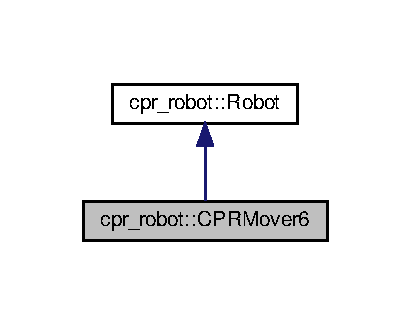
\includegraphics[width=197pt]{classcpr__robot_1_1CPRMover6__inherit__graph}
\end{center}
\end{figure}
\subsection*{Public Member Functions}
\begin{DoxyCompactItemize}
\item 
\textbf{ C\+P\+R\+Mover6} ()
\item 
virtual \textbf{ $\sim$\+C\+P\+R\+Mover6} ()
\end{DoxyCompactItemize}
\subsection*{Additional Inherited Members}


\subsection{Detailed Description}
Class representing a Mover6 robot from Commonplace Robotics GmbH. 

All model specific parameters are handled by this class 

Definition at line 9 of file C\+P\+R\+Mover6.\+h.



\subsection{Constructor \& Destructor Documentation}
\mbox{\label{classcpr__robot_1_1CPRMover6_a884cfcd259229e56f5f7d93452cf576f}} 
\index{cpr\+\_\+robot\+::\+C\+P\+R\+Mover6@{cpr\+\_\+robot\+::\+C\+P\+R\+Mover6}!C\+P\+R\+Mover6@{C\+P\+R\+Mover6}}
\index{C\+P\+R\+Mover6@{C\+P\+R\+Mover6}!cpr\+\_\+robot\+::\+C\+P\+R\+Mover6@{cpr\+\_\+robot\+::\+C\+P\+R\+Mover6}}
\subsubsection{C\+P\+R\+Mover6()}
{\footnotesize\ttfamily cpr\+\_\+robot\+::\+C\+P\+R\+Mover6\+::\+C\+P\+R\+Mover6 (\begin{DoxyParamCaption}{ }\end{DoxyParamCaption})}



Definition at line 6 of file C\+P\+R\+Mover6.\+cpp.

\mbox{\label{classcpr__robot_1_1CPRMover6_a51997dede61107c24cd6946bab6efcdb}} 
\index{cpr\+\_\+robot\+::\+C\+P\+R\+Mover6@{cpr\+\_\+robot\+::\+C\+P\+R\+Mover6}!````~C\+P\+R\+Mover6@{$\sim$\+C\+P\+R\+Mover6}}
\index{````~C\+P\+R\+Mover6@{$\sim$\+C\+P\+R\+Mover6}!cpr\+\_\+robot\+::\+C\+P\+R\+Mover6@{cpr\+\_\+robot\+::\+C\+P\+R\+Mover6}}
\subsubsection{$\sim$\+C\+P\+R\+Mover6()}
{\footnotesize\ttfamily cpr\+\_\+robot\+::\+C\+P\+R\+Mover6\+::$\sim$\+C\+P\+R\+Mover6 (\begin{DoxyParamCaption}{ }\end{DoxyParamCaption})\hspace{0.3cm}{\ttfamily [virtual]}}



Definition at line 54 of file C\+P\+R\+Mover6.\+cpp.



The documentation for this class was generated from the following files\+:\begin{DoxyCompactItemize}
\item 
\textbf{ C\+P\+R\+Mover6.\+h}\item 
\textbf{ C\+P\+R\+Mover6.\+cpp}\end{DoxyCompactItemize}

\section{cpr\+\_\+robot\+:\+:igus\+\_\+4\+D\+O\+F\+\_\+\+SV Class Reference}
\label{classcpr__robot_1_1igus__4DOF__SV}\index{cpr\+\_\+robot\+::igus\+\_\+4\+D\+O\+F\+\_\+\+SV@{cpr\+\_\+robot\+::igus\+\_\+4\+D\+O\+F\+\_\+\+SV}}


Class representing a robolink 4\+D\+OF small version robot from igus.  




{\ttfamily \#include $<$cpr\+\_\+robot.\+h$>$}



Inheritance diagram for cpr\+\_\+robot\+:\+:igus\+\_\+4\+D\+O\+F\+\_\+\+SV\+:
\nopagebreak
\begin{figure}[H]
\begin{center}
\leavevmode
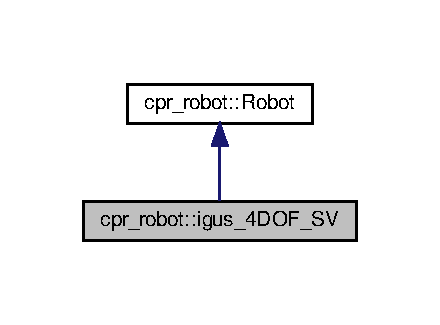
\includegraphics[width=211pt]{classcpr__robot_1_1igus__4DOF__SV__inherit__graph}
\end{center}
\end{figure}
\subsection*{Public Member Functions}
\begin{DoxyCompactItemize}
\item 
\textbf{ igus\+\_\+4\+D\+O\+F\+\_\+\+SV} ()
\begin{DoxyCompactList}\small\item\em All model specific parameters, like gear ratios, position ranges, etc. are set during construction. \end{DoxyCompactList}\item 
virtual \textbf{ $\sim$igus\+\_\+4\+D\+O\+F\+\_\+\+SV} ()
\begin{DoxyCompactList}\small\item\em Destructs an instance of the \doxyref{igus\+\_\+4\+D\+O\+F\+\_\+\+SV}{p.}{classcpr__robot_1_1igus__4DOF__SV} class. \end{DoxyCompactList}\end{DoxyCompactItemize}
\subsection*{Additional Inherited Members}


\subsection{Detailed Description}
Class representing a robolink 4\+D\+OF small version robot from igus. 

All model specific parameters are handled by this class 

Definition at line 9 of file igus\+\_\+4\+D\+O\+F\+\_\+\+S\+V.\+h.



\subsection{Constructor \& Destructor Documentation}
\mbox{\label{classcpr__robot_1_1igus__4DOF__SV_a9124672ebfca9702e9195cfc848c573e}} 
\index{cpr\+\_\+robot\+::igus\+\_\+4\+D\+O\+F\+\_\+\+SV@{cpr\+\_\+robot\+::igus\+\_\+4\+D\+O\+F\+\_\+\+SV}!igus\+\_\+4\+D\+O\+F\+\_\+\+SV@{igus\+\_\+4\+D\+O\+F\+\_\+\+SV}}
\index{igus\+\_\+4\+D\+O\+F\+\_\+\+SV@{igus\+\_\+4\+D\+O\+F\+\_\+\+SV}!cpr\+\_\+robot\+::igus\+\_\+4\+D\+O\+F\+\_\+\+SV@{cpr\+\_\+robot\+::igus\+\_\+4\+D\+O\+F\+\_\+\+SV}}
\subsubsection{igus\+\_\+4\+D\+O\+F\+\_\+\+S\+V()}
{\footnotesize\ttfamily cpr\+\_\+robot\+::igus\+\_\+4\+D\+O\+F\+\_\+\+S\+V\+::igus\+\_\+4\+D\+O\+F\+\_\+\+SV (\begin{DoxyParamCaption}{ }\end{DoxyParamCaption})}



All model specific parameters, like gear ratios, position ranges, etc. are set during construction. 



Definition at line 7 of file igus\+\_\+4\+D\+O\+F\+\_\+\+S\+V.\+cpp.

\mbox{\label{classcpr__robot_1_1igus__4DOF__SV_a0ca58340a4e481a1624c9a4549c6bf7c}} 
\index{cpr\+\_\+robot\+::igus\+\_\+4\+D\+O\+F\+\_\+\+SV@{cpr\+\_\+robot\+::igus\+\_\+4\+D\+O\+F\+\_\+\+SV}!````~igus\+\_\+4\+D\+O\+F\+\_\+\+SV@{$\sim$igus\+\_\+4\+D\+O\+F\+\_\+\+SV}}
\index{````~igus\+\_\+4\+D\+O\+F\+\_\+\+SV@{$\sim$igus\+\_\+4\+D\+O\+F\+\_\+\+SV}!cpr\+\_\+robot\+::igus\+\_\+4\+D\+O\+F\+\_\+\+SV@{cpr\+\_\+robot\+::igus\+\_\+4\+D\+O\+F\+\_\+\+SV}}
\subsubsection{$\sim$igus\+\_\+4\+D\+O\+F\+\_\+\+S\+V()}
{\footnotesize\ttfamily cpr\+\_\+robot\+::igus\+\_\+4\+D\+O\+F\+\_\+\+S\+V\+::$\sim$igus\+\_\+4\+D\+O\+F\+\_\+\+SV (\begin{DoxyParamCaption}{ }\end{DoxyParamCaption})\hspace{0.3cm}{\ttfamily [virtual]}}



Destructs an instance of the \doxyref{igus\+\_\+4\+D\+O\+F\+\_\+\+SV}{p.}{classcpr__robot_1_1igus__4DOF__SV} class. 



Definition at line 42 of file igus\+\_\+4\+D\+O\+F\+\_\+\+S\+V.\+cpp.



The documentation for this class was generated from the following files\+:\begin{DoxyCompactItemize}
\item 
\textbf{ igus\+\_\+4\+D\+O\+F\+\_\+\+S\+V.\+h}\item 
\textbf{ igus\+\_\+4\+D\+O\+F\+\_\+\+S\+V.\+cpp}\end{DoxyCompactItemize}

\section{cpr\+\_\+robot\+:\+:igus\+\_\+5\+D\+O\+F\+\_\+\+SV Class Reference}
\label{classcpr__robot_1_1igus__5DOF__SV}\index{cpr\+\_\+robot\+::igus\+\_\+5\+D\+O\+F\+\_\+\+SV@{cpr\+\_\+robot\+::igus\+\_\+5\+D\+O\+F\+\_\+\+SV}}


Class representing a robolink 5\+D\+OF small version robot from igus.  




{\ttfamily \#include $<$cpr\+\_\+robot.\+h$>$}



Inheritance diagram for cpr\+\_\+robot\+:\+:igus\+\_\+5\+D\+O\+F\+\_\+\+SV\+:
\nopagebreak
\begin{figure}[H]
\begin{center}
\leavevmode
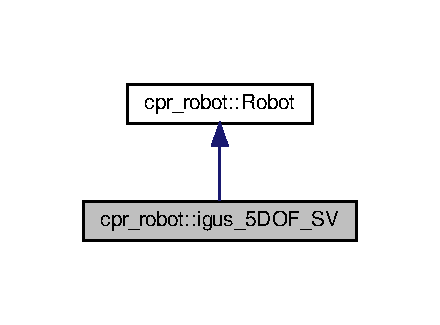
\includegraphics[width=211pt]{classcpr__robot_1_1igus__5DOF__SV__inherit__graph}
\end{center}
\end{figure}
\subsection*{Public Member Functions}
\begin{DoxyCompactItemize}
\item 
\textbf{ igus\+\_\+5\+D\+O\+F\+\_\+\+SV} ()
\begin{DoxyCompactList}\small\item\em All model specific parameters, like gear ratios, position ranges, etc. are set during construction. \end{DoxyCompactList}\item 
virtual \textbf{ $\sim$igus\+\_\+5\+D\+O\+F\+\_\+\+SV} ()
\begin{DoxyCompactList}\small\item\em Destructs an instance of the \doxyref{igus\+\_\+5\+D\+O\+F\+\_\+\+SV}{p.}{classcpr__robot_1_1igus__5DOF__SV} class. \end{DoxyCompactList}\end{DoxyCompactItemize}
\subsection*{Additional Inherited Members}


\subsection{Detailed Description}
Class representing a robolink 5\+D\+OF small version robot from igus. 

All model specific parameters are handled by this class 

Definition at line 9 of file igus\+\_\+5\+D\+O\+F\+\_\+\+S\+V.\+h.



\subsection{Constructor \& Destructor Documentation}
\mbox{\label{classcpr__robot_1_1igus__5DOF__SV_a24334d6d98154e921b7a795572e6fbac}} 
\index{cpr\+\_\+robot\+::igus\+\_\+5\+D\+O\+F\+\_\+\+SV@{cpr\+\_\+robot\+::igus\+\_\+5\+D\+O\+F\+\_\+\+SV}!igus\+\_\+5\+D\+O\+F\+\_\+\+SV@{igus\+\_\+5\+D\+O\+F\+\_\+\+SV}}
\index{igus\+\_\+5\+D\+O\+F\+\_\+\+SV@{igus\+\_\+5\+D\+O\+F\+\_\+\+SV}!cpr\+\_\+robot\+::igus\+\_\+5\+D\+O\+F\+\_\+\+SV@{cpr\+\_\+robot\+::igus\+\_\+5\+D\+O\+F\+\_\+\+SV}}
\subsubsection{igus\+\_\+5\+D\+O\+F\+\_\+\+S\+V()}
{\footnotesize\ttfamily cpr\+\_\+robot\+::igus\+\_\+5\+D\+O\+F\+\_\+\+S\+V\+::igus\+\_\+5\+D\+O\+F\+\_\+\+SV (\begin{DoxyParamCaption}{ }\end{DoxyParamCaption})}



All model specific parameters, like gear ratios, position ranges, etc. are set during construction. 



Definition at line 7 of file igus\+\_\+5\+D\+O\+F\+\_\+\+S\+V.\+cpp.

\mbox{\label{classcpr__robot_1_1igus__5DOF__SV_a19763f0d9f9c8045e03b1e0fc35282c3}} 
\index{cpr\+\_\+robot\+::igus\+\_\+5\+D\+O\+F\+\_\+\+SV@{cpr\+\_\+robot\+::igus\+\_\+5\+D\+O\+F\+\_\+\+SV}!````~igus\+\_\+5\+D\+O\+F\+\_\+\+SV@{$\sim$igus\+\_\+5\+D\+O\+F\+\_\+\+SV}}
\index{````~igus\+\_\+5\+D\+O\+F\+\_\+\+SV@{$\sim$igus\+\_\+5\+D\+O\+F\+\_\+\+SV}!cpr\+\_\+robot\+::igus\+\_\+5\+D\+O\+F\+\_\+\+SV@{cpr\+\_\+robot\+::igus\+\_\+5\+D\+O\+F\+\_\+\+SV}}
\subsubsection{$\sim$igus\+\_\+5\+D\+O\+F\+\_\+\+S\+V()}
{\footnotesize\ttfamily cpr\+\_\+robot\+::igus\+\_\+5\+D\+O\+F\+\_\+\+S\+V\+::$\sim$igus\+\_\+5\+D\+O\+F\+\_\+\+SV (\begin{DoxyParamCaption}{ }\end{DoxyParamCaption})\hspace{0.3cm}{\ttfamily [virtual]}}



Destructs an instance of the \doxyref{igus\+\_\+5\+D\+O\+F\+\_\+\+SV}{p.}{classcpr__robot_1_1igus__5DOF__SV} class. 



Definition at line 49 of file igus\+\_\+5\+D\+O\+F\+\_\+\+S\+V.\+cpp.



The documentation for this class was generated from the following files\+:\begin{DoxyCompactItemize}
\item 
\textbf{ igus\+\_\+5\+D\+O\+F\+\_\+\+S\+V.\+h}\item 
\textbf{ igus\+\_\+5\+D\+O\+F\+\_\+\+S\+V.\+cpp}\end{DoxyCompactItemize}

\section{cpr\+\_\+robot\+:\+:Joint Class Reference}
\label{classcpr__robot_1_1Joint}\index{cpr\+\_\+robot\+::\+Joint@{cpr\+\_\+robot\+::\+Joint}}


Represents a single joint of a robot.  




{\ttfamily \#include $<$cpr\+\_\+robot.\+h$>$}

\subsection*{Public Member Functions}
\begin{DoxyCompactItemize}
\item 
void \textbf{ Disable\+Motor} ()
\begin{DoxyCompactList}\small\item\em Will send a command to disable motor motion to the firmware of the module that is controlling the motor of the joint. \end{DoxyCompactList}\item 
void \textbf{ Enable\+Motor} ()
\begin{DoxyCompactList}\small\item\em Will send a command to enable motor motion to the firmware of the module that is controlling the motor of the joint. \end{DoxyCompactList}\item 
double \textbf{ get\+\_\+\+Current\+Effort} () const
\begin{DoxyCompactList}\small\item\em Gets the effort that is put into moving the joing. Currently not implemented. \end{DoxyCompactList}\item 
double \textbf{ get\+\_\+\+Current\+Position} () const
\begin{DoxyCompactList}\small\item\em Gets the current position of the joint. \end{DoxyCompactList}\item 
double \textbf{ get\+\_\+\+Current\+Velocity} () const
\begin{DoxyCompactList}\small\item\em Gets the current angular velocity of the joint. \end{DoxyCompactList}\item 
double \textbf{ get\+\_\+\+Desired\+Velocity} () const
\begin{DoxyCompactList}\small\item\em Gets the desired angular velocity of the joint. \end{DoxyCompactList}\item 
uint8\+\_\+t \textbf{ get\+\_\+\+Error\+Flags} () const
\begin{DoxyCompactList}\small\item\em Gets the error flags that are currently reported by the firmware in the module that is controlling the motor of the joint. \end{DoxyCompactList}\item 
double \textbf{ get\+\_\+\+Gear\+Ratio} () const
\begin{DoxyCompactList}\small\item\em Gets the current gear ratio that is used during conversion from encoder position to joint position. \end{DoxyCompactList}\item 
bool \textbf{ get\+\_\+\+Is\+Referenced} () const
\begin{DoxyCompactList}\small\item\em Allows to determine if the joint has been referenced. \end{DoxyCompactList}\item 
const std\+::string \& \textbf{ get\+\_\+\+Joint\+Name} () const
\begin{DoxyCompactList}\small\item\em Gets the name of the joint used when communicating over R\+OS topics and services. \end{DoxyCompactList}\item 
double \textbf{ get\+\_\+\+Max\+Position} () const
\begin{DoxyCompactList}\small\item\em Gets the upper position bound of the joint. \end{DoxyCompactList}\item 
double \textbf{ get\+\_\+\+Max\+Veclocity} () const
\begin{DoxyCompactList}\small\item\em Gets the maximum allowed angular velocity of the joint. \end{DoxyCompactList}\item 
double \textbf{ get\+\_\+\+Min\+Position} () const
\begin{DoxyCompactList}\small\item\em Gets the lower position bound of the joint. \end{DoxyCompactList}\item 
int32\+\_\+t \textbf{ get\+\_\+\+Motor\+Offset} () const
\begin{DoxyCompactList}\small\item\em Gets the zero position of the motor. \end{DoxyCompactList}\item 
int32\+\_\+t \textbf{ get\+\_\+\+Ticks\+Per\+Motor\+Rotation} () const
\begin{DoxyCompactList}\small\item\em Gets the current number of ticks per motor rotation used during conversion from encoder position to joint position. \end{DoxyCompactList}\item 
void \textbf{ Init} ()
\begin{DoxyCompactList}\small\item\em Initializes the joint. \end{DoxyCompactList}\item 
\textbf{ Joint} (\textbf{ Bus} \&can\+Bus, const uint32\+\_\+t module\+Id)
\begin{DoxyCompactList}\small\item\em Constructs an instance of the \doxyref{Joint}{p.}{classcpr__robot_1_1Joint} class. \end{DoxyCompactList}\item 
void \textbf{ Publish\+State} (sensor\+\_\+msgs\+::\+Joint\+State \&msg)
\begin{DoxyCompactList}\small\item\em Used when publishing joint states. \end{DoxyCompactList}\item 
void \textbf{ Read} ()
\begin{DoxyCompactList}\small\item\em Reads the current state of the joint from the firmware in the module that is controlling the motor of the joint. \end{DoxyCompactList}\item 
void \textbf{ set\+\_\+\+Gear\+Ratio} (const double ratio)
\begin{DoxyCompactList}\small\item\em Sets the current gear ratio that is used during conversion from encoder position to joint position. \end{DoxyCompactList}\item 
void \textbf{ set\+\_\+\+Joint\+Name} (const std\+::string \&joint\+Name)
\begin{DoxyCompactList}\small\item\em Sets the name of the joint used when communicating over R\+OS topics and services. \end{DoxyCompactList}\item 
void \textbf{ set\+\_\+\+Max\+Position} (const double position)
\begin{DoxyCompactList}\small\item\em Sets the upper position bound of the joint. \end{DoxyCompactList}\item 
void \textbf{ set\+\_\+\+Max\+Velocity} (const double velocity)
\begin{DoxyCompactList}\small\item\em Sets the maximum allowed angular velocity of the joint. \end{DoxyCompactList}\item 
void \textbf{ set\+\_\+\+Min\+Position} (const double position)
\begin{DoxyCompactList}\small\item\em Sets the lower position bound of the joint. \end{DoxyCompactList}\item 
void \textbf{ set\+\_\+\+Motor\+Offset} (const int32\+\_\+t ticks)
\begin{DoxyCompactList}\small\item\em Sets the zero position of the motor. \end{DoxyCompactList}\item 
void \textbf{ set\+\_\+\+Ticks\+Per\+Motor\+Rotation} (const int32\+\_\+t ticks)
\begin{DoxyCompactList}\small\item\em Sets the current number of ticks per motor rotation used during conversion from encoder position to joint position. \end{DoxyCompactList}\item 
void \textbf{ Set\+Zero} ()
\begin{DoxyCompactList}\small\item\em Will send a command to reset the encoder position for the joint to the firmware of the module that is controlling the motor of the joint. \end{DoxyCompactList}\item 
void \textbf{ Start} ()
\begin{DoxyCompactList}\small\item\em Will start the communication with the firmware of the module that is controlling the motor of the joint. \end{DoxyCompactList}\item 
void \textbf{ Start\+Referencing} ()
\begin{DoxyCompactList}\small\item\em Will send a command to begin the referencing procedure for the joint to the firmware of the module that is controlling the motor of the joint. \end{DoxyCompactList}\item 
void \textbf{ Stop} ()
\begin{DoxyCompactList}\small\item\em Will stop the communication with the firmware of the module that is controlling the motor of the joint. \end{DoxyCompactList}\item 
void \textbf{ Write} (double override)
\begin{DoxyCompactList}\small\item\em Sends the current motion commands to the firmware in the module that is controlling the motor of the joint. \end{DoxyCompactList}\item 
virtual \textbf{ $\sim$\+Joint} ()
\begin{DoxyCompactList}\small\item\em The destructor of the \doxyref{Joint}{p.}{classcpr__robot_1_1Joint} class. \end{DoxyCompactList}\end{DoxyCompactItemize}
\subsection*{Static Public Attributes}
\begin{DoxyCompactItemize}
\item 
static constexpr uint8\+\_\+t \textbf{ D\+A\+T\+A\+B\+I\+T\+\_\+\+R\+E\+F\+E\+R\+E\+N\+C\+ED} =0x80
\begin{DoxyCompactList}\small\item\em Status bit indicating that the joint has been referenced. \end{DoxyCompactList}\end{DoxyCompactItemize}
\subsection*{Protected Member Functions}
\begin{DoxyCompactItemize}
\item 
virtual void \textbf{ On\+Init} ()
\begin{DoxyCompactList}\small\item\em Initialization. Should only be called after the parameters (gear ratio, ticks per motor rotation) have been set. \end{DoxyCompactList}\item 
virtual void \textbf{ On\+Read} ()
\begin{DoxyCompactList}\small\item\em Reads the current state of the joint from the firmware. \end{DoxyCompactList}\item 
virtual void \textbf{ On\+Write} (double override)
\begin{DoxyCompactList}\small\item\em Sends the current motion commands to the firmware in the module that is controlling the motor of the joint. This virtual function is intended to be overridable by derived classes, but should then be called from the override. \end{DoxyCompactList}\item 
int32\+\_\+t \textbf{ Position\+To\+Ticks} (const double position) const
\begin{DoxyCompactList}\small\item\em Converts a joint position to a motor position. \end{DoxyCompactList}\item 
double \textbf{ Ticks\+To\+Position} (const int32\+\_\+t ticks) const
\begin{DoxyCompactList}\small\item\em Converts a motor position to a joint position. \end{DoxyCompactList}\end{DoxyCompactItemize}
\subsection*{Private Member Functions}
\begin{DoxyCompactItemize}
\item 
void \textbf{ Joint\+Jog\+Callback} (const control\+\_\+msgs\+::\+Joint\+Jog \&msg)
\begin{DoxyCompactList}\small\item\em Callback for received messages on the /\+Joint\+Jog R\+OS topic. \end{DoxyCompactList}\item 
double \textbf{ Read\+Position} (uint8\+\_\+t \&time\+Stamp, std\+::chrono\+::high\+\_\+resolution\+\_\+clock\+::time\+\_\+point \&reception\+Time, uint8\+\_\+t \&error\+Flags, uint8\+\_\+t \&data\+Bits)
\begin{DoxyCompactList}\small\item\em Returns the position of the joint according to the last update received from the firmware that is controlling the motor of the joint. \end{DoxyCompactList}\end{DoxyCompactItemize}
\subsection*{Private Attributes}
\begin{DoxyCompactItemize}
\item 
bool \textbf{ m\+\_\+b\+Referenced}
\begin{DoxyCompactList}\small\item\em Flag indicating whether the joint is reported as referenced by the firmware. \end{DoxyCompactList}\item 
double \textbf{ m\+\_\+\+Current\+Effort}
\begin{DoxyCompactList}\small\item\em Reserved for future use with closed loop joints. Currently always zero. \end{DoxyCompactList}\item 
double \textbf{ m\+\_\+\+Current\+Position}
\begin{DoxyCompactList}\small\item\em The current position of the joint computed from the encoder position and joint parameters in degrees. \end{DoxyCompactList}\item 
double \textbf{ m\+\_\+\+Current\+Velocity}
\begin{DoxyCompactList}\small\item\em The current angular velocity of the joint computed from the change in encoder position and joint parameters in degrees per second. \end{DoxyCompactList}\item 
double \textbf{ m\+\_\+\+Desired\+Velocity}
\begin{DoxyCompactList}\small\item\em The desired angular velocity of the joint in radians per second. \end{DoxyCompactList}\item 
uint8\+\_\+t \textbf{ m\+\_\+\+Error\+Flags}
\begin{DoxyCompactList}\small\item\em The error flags reported by the firmware of the module that is controlling the joint. \end{DoxyCompactList}\item 
double \textbf{ m\+\_\+\+Gear\+Ratio}
\begin{DoxyCompactList}\small\item\em The total gear ratio of the joint. \end{DoxyCompactList}\item 
ros\+::\+Subscriber \textbf{ m\+\_\+\+Joint\+Jog\+Subscriber}
\begin{DoxyCompactList}\small\item\em The R\+OS subscriber for the /\+Joint\+Jog topic which will receive jog messages. \end{DoxyCompactList}\item 
std\+::string \textbf{ m\+\_\+\+Joint\+Name}
\begin{DoxyCompactList}\small\item\em The name used for this joint when communicating over R\+OS topics and services. \end{DoxyCompactList}\item 
uint8\+\_\+t \textbf{ m\+\_\+\+Last\+Time\+Stamp}
\begin{DoxyCompactList}\small\item\em The timestamp of the last status message received from the firmware in the module that is controlling the joint. \end{DoxyCompactList}\item 
std\+::chrono\+::high\+\_\+resolution\+\_\+clock\+::time\+\_\+point \textbf{ m\+\_\+\+Last\+Update}
\begin{DoxyCompactList}\small\item\em The time at which the last status message has been received from the firmware in the module that is controlling the joint. \end{DoxyCompactList}\item 
double \textbf{ m\+\_\+\+Max\+Velocity}
\begin{DoxyCompactList}\small\item\em The maximum angular velocity of the joint in radians per second. \end{DoxyCompactList}\item 
ros\+::\+Node\+Handle \textbf{ m\+\_\+\+Node}
\begin{DoxyCompactList}\small\item\em A handle to the current R\+OS node. \end{DoxyCompactList}\item 
\textbf{ Motor\+Module} $\ast$ \textbf{ m\+\_\+p\+Module}
\begin{DoxyCompactList}\small\item\em Pointer to an instance of the \doxyref{Motor\+Module}{p.}{classcpr__robot_1_1MotorModule} class which represents the module and firmware driving the motor for the joint. \end{DoxyCompactList}\item 
int32\+\_\+t \textbf{ m\+\_\+\+Ticks\+Per\+Motor\+Rotation}
\begin{DoxyCompactList}\small\item\em The number of encoder ticks representing exactly one rotation of the motor that is driving this joint. \end{DoxyCompactList}\end{DoxyCompactItemize}


\subsection{Detailed Description}
Represents a single joint of a robot. 

This class contains information about the current state of the joint (position, speed) as well as the parameters for the joint (gear ratio, ticks per motor rotation). Conversion between encoder ticks and the actual position of the joint (measured in degrees) is done by this class. 

Definition at line 9 of file Joint.\+h.



\subsection{Constructor \& Destructor Documentation}
\mbox{\label{classcpr__robot_1_1Joint_a624d26c85789eada0b78d4748ec53d31}} 
\index{cpr\+\_\+robot\+::\+Joint@{cpr\+\_\+robot\+::\+Joint}!Joint@{Joint}}
\index{Joint@{Joint}!cpr\+\_\+robot\+::\+Joint@{cpr\+\_\+robot\+::\+Joint}}
\subsubsection{Joint()}
{\footnotesize\ttfamily cpr\+\_\+robot\+::\+Joint\+::\+Joint (\begin{DoxyParamCaption}\item[{\textbf{ Bus} \&}]{can\+Bus,  }\item[{const uint32\+\_\+t}]{module\+Id }\end{DoxyParamCaption})}



Constructs an instance of the \doxyref{Joint}{p.}{classcpr__robot_1_1Joint} class. 


\begin{DoxyParams}{Parameters}
{\em can\+Bus} & An instance of the \doxyref{Bus}{p.}{classcpr__robot_1_1Bus} class which will be used for communication with the firmware in the module that is controlling the motor of the joint. \\
\hline
{\em module\+Id} & The Id of the module that is controlling the motor of this joint. \\
\hline
\end{DoxyParams}


Definition at line 10 of file Joint.\+cpp.

\mbox{\label{classcpr__robot_1_1Joint_a899b6077763552761845ab31f79214a1}} 
\index{cpr\+\_\+robot\+::\+Joint@{cpr\+\_\+robot\+::\+Joint}!````~Joint@{$\sim$\+Joint}}
\index{````~Joint@{$\sim$\+Joint}!cpr\+\_\+robot\+::\+Joint@{cpr\+\_\+robot\+::\+Joint}}
\subsubsection{$\sim$\+Joint()}
{\footnotesize\ttfamily cpr\+\_\+robot\+::\+Joint\+::$\sim$\+Joint (\begin{DoxyParamCaption}{ }\end{DoxyParamCaption})\hspace{0.3cm}{\ttfamily [virtual]}}



The destructor of the \doxyref{Joint}{p.}{classcpr__robot_1_1Joint} class. 



Definition at line 35 of file Joint.\+cpp.



\subsection{Member Function Documentation}
\mbox{\label{classcpr__robot_1_1Joint_a2cd4f2b6f903b9dc0a1c0efdd3730ebc}} 
\index{cpr\+\_\+robot\+::\+Joint@{cpr\+\_\+robot\+::\+Joint}!Disable\+Motor@{Disable\+Motor}}
\index{Disable\+Motor@{Disable\+Motor}!cpr\+\_\+robot\+::\+Joint@{cpr\+\_\+robot\+::\+Joint}}
\subsubsection{Disable\+Motor()}
{\footnotesize\ttfamily void cpr\+\_\+robot\+::\+Joint\+::\+Disable\+Motor (\begin{DoxyParamCaption}{ }\end{DoxyParamCaption})}



Will send a command to disable motor motion to the firmware of the module that is controlling the motor of the joint. 



Definition at line 317 of file Joint.\+cpp.

\mbox{\label{classcpr__robot_1_1Joint_a0525e748656f30822b053cada12a5c28}} 
\index{cpr\+\_\+robot\+::\+Joint@{cpr\+\_\+robot\+::\+Joint}!Enable\+Motor@{Enable\+Motor}}
\index{Enable\+Motor@{Enable\+Motor}!cpr\+\_\+robot\+::\+Joint@{cpr\+\_\+robot\+::\+Joint}}
\subsubsection{Enable\+Motor()}
{\footnotesize\ttfamily void cpr\+\_\+robot\+::\+Joint\+::\+Enable\+Motor (\begin{DoxyParamCaption}{ }\end{DoxyParamCaption})}



Will send a command to enable motor motion to the firmware of the module that is controlling the motor of the joint. 



Definition at line 311 of file Joint.\+cpp.

\mbox{\label{classcpr__robot_1_1Joint_ac03ee9878d68ac22e206141a49af61f1}} 
\index{cpr\+\_\+robot\+::\+Joint@{cpr\+\_\+robot\+::\+Joint}!get\+\_\+\+Current\+Effort@{get\+\_\+\+Current\+Effort}}
\index{get\+\_\+\+Current\+Effort@{get\+\_\+\+Current\+Effort}!cpr\+\_\+robot\+::\+Joint@{cpr\+\_\+robot\+::\+Joint}}
\subsubsection{get\+\_\+\+Current\+Effort()}
{\footnotesize\ttfamily double cpr\+\_\+robot\+::\+Joint\+::get\+\_\+\+Current\+Effort (\begin{DoxyParamCaption}{ }\end{DoxyParamCaption}) const}



Gets the effort that is put into moving the joing. Currently not implemented. 

\begin{DoxyReturn}{Returns}
Always returns zero. 
\end{DoxyReturn}


Definition at line 70 of file Joint.\+cpp.

\mbox{\label{classcpr__robot_1_1Joint_a8e570ed99b9e53ac085ec9fadd35eaa9}} 
\index{cpr\+\_\+robot\+::\+Joint@{cpr\+\_\+robot\+::\+Joint}!get\+\_\+\+Current\+Position@{get\+\_\+\+Current\+Position}}
\index{get\+\_\+\+Current\+Position@{get\+\_\+\+Current\+Position}!cpr\+\_\+robot\+::\+Joint@{cpr\+\_\+robot\+::\+Joint}}
\subsubsection{get\+\_\+\+Current\+Position()}
{\footnotesize\ttfamily double cpr\+\_\+robot\+::\+Joint\+::get\+\_\+\+Current\+Position (\begin{DoxyParamCaption}{ }\end{DoxyParamCaption}) const}



Gets the current position of the joint. 

\begin{DoxyReturn}{Returns}
The current position in degrees. 
\end{DoxyReturn}


Definition at line 56 of file Joint.\+cpp.

\mbox{\label{classcpr__robot_1_1Joint_a140b26d969f491c8242231aefa634634}} 
\index{cpr\+\_\+robot\+::\+Joint@{cpr\+\_\+robot\+::\+Joint}!get\+\_\+\+Current\+Velocity@{get\+\_\+\+Current\+Velocity}}
\index{get\+\_\+\+Current\+Velocity@{get\+\_\+\+Current\+Velocity}!cpr\+\_\+robot\+::\+Joint@{cpr\+\_\+robot\+::\+Joint}}
\subsubsection{get\+\_\+\+Current\+Velocity()}
{\footnotesize\ttfamily double cpr\+\_\+robot\+::\+Joint\+::get\+\_\+\+Current\+Velocity (\begin{DoxyParamCaption}{ }\end{DoxyParamCaption}) const}



Gets the current angular velocity of the joint. 

\begin{DoxyReturn}{Returns}
The current angular velocity in degrees per second. 
\end{DoxyReturn}


Definition at line 63 of file Joint.\+cpp.

\mbox{\label{classcpr__robot_1_1Joint_a3578f2c7039da34d4c9c14697aea345f}} 
\index{cpr\+\_\+robot\+::\+Joint@{cpr\+\_\+robot\+::\+Joint}!get\+\_\+\+Desired\+Velocity@{get\+\_\+\+Desired\+Velocity}}
\index{get\+\_\+\+Desired\+Velocity@{get\+\_\+\+Desired\+Velocity}!cpr\+\_\+robot\+::\+Joint@{cpr\+\_\+robot\+::\+Joint}}
\subsubsection{get\+\_\+\+Desired\+Velocity()}
{\footnotesize\ttfamily double cpr\+\_\+robot\+::\+Joint\+::get\+\_\+\+Desired\+Velocity (\begin{DoxyParamCaption}{ }\end{DoxyParamCaption}) const}



Gets the desired angular velocity of the joint. 

\begin{DoxyReturn}{Returns}
The desired angular velocity in degrees per second. 
\end{DoxyReturn}


Definition at line 107 of file Joint.\+cpp.

\mbox{\label{classcpr__robot_1_1Joint_aa67b65fe13b6d43f97faf8d97aa2420f}} 
\index{cpr\+\_\+robot\+::\+Joint@{cpr\+\_\+robot\+::\+Joint}!get\+\_\+\+Error\+Flags@{get\+\_\+\+Error\+Flags}}
\index{get\+\_\+\+Error\+Flags@{get\+\_\+\+Error\+Flags}!cpr\+\_\+robot\+::\+Joint@{cpr\+\_\+robot\+::\+Joint}}
\subsubsection{get\+\_\+\+Error\+Flags()}
{\footnotesize\ttfamily uint8\+\_\+t cpr\+\_\+robot\+::\+Joint\+::get\+\_\+\+Error\+Flags (\begin{DoxyParamCaption}{ }\end{DoxyParamCaption}) const}



Gets the error flags that are currently reported by the firmware in the module that is controlling the motor of the joint. 

\begin{DoxyReturn}{Returns}
Bitfield with the error flags. 
\end{DoxyReturn}


Definition at line 193 of file Joint.\+cpp.

\mbox{\label{classcpr__robot_1_1Joint_a78b3ad1e3f1a6530ff7aca0268eebf95}} 
\index{cpr\+\_\+robot\+::\+Joint@{cpr\+\_\+robot\+::\+Joint}!get\+\_\+\+Gear\+Ratio@{get\+\_\+\+Gear\+Ratio}}
\index{get\+\_\+\+Gear\+Ratio@{get\+\_\+\+Gear\+Ratio}!cpr\+\_\+robot\+::\+Joint@{cpr\+\_\+robot\+::\+Joint}}
\subsubsection{get\+\_\+\+Gear\+Ratio()}
{\footnotesize\ttfamily double cpr\+\_\+robot\+::\+Joint\+::get\+\_\+\+Gear\+Ratio (\begin{DoxyParamCaption}{ }\end{DoxyParamCaption}) const}



Gets the current gear ratio that is used during conversion from encoder position to joint position. 

\begin{DoxyReturn}{Returns}
Current gear ratio. 
\end{DoxyReturn}


Definition at line 298 of file Joint.\+cpp.

\mbox{\label{classcpr__robot_1_1Joint_a438a490b29b4b19817f2a2b8948ad3bd}} 
\index{cpr\+\_\+robot\+::\+Joint@{cpr\+\_\+robot\+::\+Joint}!get\+\_\+\+Is\+Referenced@{get\+\_\+\+Is\+Referenced}}
\index{get\+\_\+\+Is\+Referenced@{get\+\_\+\+Is\+Referenced}!cpr\+\_\+robot\+::\+Joint@{cpr\+\_\+robot\+::\+Joint}}
\subsubsection{get\+\_\+\+Is\+Referenced()}
{\footnotesize\ttfamily bool cpr\+\_\+robot\+::\+Joint\+::get\+\_\+\+Is\+Referenced (\begin{DoxyParamCaption}{ }\end{DoxyParamCaption}) const}



Allows to determine if the joint has been referenced. 

\begin{DoxyReturn}{Returns}
If the joint is reported as referenced by the firmware returns true, elsewise false. 
\end{DoxyReturn}


Definition at line 29 of file Joint.\+cpp.

\mbox{\label{classcpr__robot_1_1Joint_a54a2c42a9f717031ca65ef96e774dc09}} 
\index{cpr\+\_\+robot\+::\+Joint@{cpr\+\_\+robot\+::\+Joint}!get\+\_\+\+Joint\+Name@{get\+\_\+\+Joint\+Name}}
\index{get\+\_\+\+Joint\+Name@{get\+\_\+\+Joint\+Name}!cpr\+\_\+robot\+::\+Joint@{cpr\+\_\+robot\+::\+Joint}}
\subsubsection{get\+\_\+\+Joint\+Name()}
{\footnotesize\ttfamily const std\+::string \& cpr\+\_\+robot\+::\+Joint\+::get\+\_\+\+Joint\+Name (\begin{DoxyParamCaption}{ }\end{DoxyParamCaption}) const}



Gets the name of the joint used when communicating over R\+OS topics and services. 

\begin{DoxyReturn}{Returns}
The name of the joint as used in message over /\+Joint\+Jog and /joint\+\_\+states R\+OS topics. 
\end{DoxyReturn}


Definition at line 42 of file Joint.\+cpp.

\mbox{\label{classcpr__robot_1_1Joint_a0acd393c18e0f4e6443e17c2e925072a}} 
\index{cpr\+\_\+robot\+::\+Joint@{cpr\+\_\+robot\+::\+Joint}!get\+\_\+\+Max\+Position@{get\+\_\+\+Max\+Position}}
\index{get\+\_\+\+Max\+Position@{get\+\_\+\+Max\+Position}!cpr\+\_\+robot\+::\+Joint@{cpr\+\_\+robot\+::\+Joint}}
\subsubsection{get\+\_\+\+Max\+Position()}
{\footnotesize\ttfamily double cpr\+\_\+robot\+::\+Joint\+::get\+\_\+\+Max\+Position (\begin{DoxyParamCaption}{ }\end{DoxyParamCaption}) const}



Gets the upper position bound of the joint. 

\begin{DoxyReturn}{Returns}
The currrent upper bound for the position of the joint in degrees. 
\end{DoxyReturn}


Definition at line 142 of file Joint.\+cpp.

\mbox{\label{classcpr__robot_1_1Joint_a87fa401b2e67be3bd622c0bed09b0fef}} 
\index{cpr\+\_\+robot\+::\+Joint@{cpr\+\_\+robot\+::\+Joint}!get\+\_\+\+Max\+Veclocity@{get\+\_\+\+Max\+Veclocity}}
\index{get\+\_\+\+Max\+Veclocity@{get\+\_\+\+Max\+Veclocity}!cpr\+\_\+robot\+::\+Joint@{cpr\+\_\+robot\+::\+Joint}}
\subsubsection{get\+\_\+\+Max\+Veclocity()}
{\footnotesize\ttfamily double cpr\+\_\+robot\+::\+Joint\+::get\+\_\+\+Max\+Veclocity (\begin{DoxyParamCaption}{ }\end{DoxyParamCaption}) const}



Gets the maximum allowed angular velocity of the joint. 

\begin{DoxyReturn}{Returns}
The currently allowed angular velocity in degrees per second. 
\end{DoxyReturn}


Definition at line 114 of file Joint.\+cpp.

\mbox{\label{classcpr__robot_1_1Joint_afd75fadedb39663cf1ed1ea2b345e315}} 
\index{cpr\+\_\+robot\+::\+Joint@{cpr\+\_\+robot\+::\+Joint}!get\+\_\+\+Min\+Position@{get\+\_\+\+Min\+Position}}
\index{get\+\_\+\+Min\+Position@{get\+\_\+\+Min\+Position}!cpr\+\_\+robot\+::\+Joint@{cpr\+\_\+robot\+::\+Joint}}
\subsubsection{get\+\_\+\+Min\+Position()}
{\footnotesize\ttfamily double cpr\+\_\+robot\+::\+Joint\+::get\+\_\+\+Min\+Position (\begin{DoxyParamCaption}{ }\end{DoxyParamCaption}) const}



Gets the lower position bound of the joint. 

\begin{DoxyReturn}{Returns}
The currrent lower bound for the position of the joint in degrees. 
\end{DoxyReturn}


Definition at line 128 of file Joint.\+cpp.

\mbox{\label{classcpr__robot_1_1Joint_a54378769e81258582e8191fc0bc16085}} 
\index{cpr\+\_\+robot\+::\+Joint@{cpr\+\_\+robot\+::\+Joint}!get\+\_\+\+Motor\+Offset@{get\+\_\+\+Motor\+Offset}}
\index{get\+\_\+\+Motor\+Offset@{get\+\_\+\+Motor\+Offset}!cpr\+\_\+robot\+::\+Joint@{cpr\+\_\+robot\+::\+Joint}}
\subsubsection{get\+\_\+\+Motor\+Offset()}
{\footnotesize\ttfamily int32\+\_\+t cpr\+\_\+robot\+::\+Joint\+::get\+\_\+\+Motor\+Offset (\begin{DoxyParamCaption}{ }\end{DoxyParamCaption}) const}



Gets the zero position of the motor. 

\begin{DoxyReturn}{Returns}
Current offset of the the zero position in encoder ticks. 
\end{DoxyReturn}


Definition at line 156 of file Joint.\+cpp.

\mbox{\label{classcpr__robot_1_1Joint_aff5043164fe4b6a8013edb265566bc6f}} 
\index{cpr\+\_\+robot\+::\+Joint@{cpr\+\_\+robot\+::\+Joint}!get\+\_\+\+Ticks\+Per\+Motor\+Rotation@{get\+\_\+\+Ticks\+Per\+Motor\+Rotation}}
\index{get\+\_\+\+Ticks\+Per\+Motor\+Rotation@{get\+\_\+\+Ticks\+Per\+Motor\+Rotation}!cpr\+\_\+robot\+::\+Joint@{cpr\+\_\+robot\+::\+Joint}}
\subsubsection{get\+\_\+\+Ticks\+Per\+Motor\+Rotation()}
{\footnotesize\ttfamily int32\+\_\+t cpr\+\_\+robot\+::\+Joint\+::get\+\_\+\+Ticks\+Per\+Motor\+Rotation (\begin{DoxyParamCaption}{ }\end{DoxyParamCaption}) const}



Gets the current number of ticks per motor rotation used during conversion from encoder position to joint position. 

\begin{DoxyReturn}{Returns}
Current number of encoder ticks representing exactly one motor rotation. 
\end{DoxyReturn}


Definition at line 284 of file Joint.\+cpp.

\mbox{\label{classcpr__robot_1_1Joint_a893c05463055ae975a60e8dbd643d288}} 
\index{cpr\+\_\+robot\+::\+Joint@{cpr\+\_\+robot\+::\+Joint}!Init@{Init}}
\index{Init@{Init}!cpr\+\_\+robot\+::\+Joint@{cpr\+\_\+robot\+::\+Joint}}
\subsubsection{Init()}
{\footnotesize\ttfamily void cpr\+\_\+robot\+::\+Joint\+::\+Init (\begin{DoxyParamCaption}{ }\end{DoxyParamCaption})}



Initializes the joint. 

Should be called after all joint parameters (gear ratio, ticks per motor rotation) have been set. Will call the virtual On\+Init method. 

Definition at line 235 of file Joint.\+cpp.

\mbox{\label{classcpr__robot_1_1Joint_a0df4c7eef1f2708d5a1df02e37d4f77d}} 
\index{cpr\+\_\+robot\+::\+Joint@{cpr\+\_\+robot\+::\+Joint}!Joint\+Jog\+Callback@{Joint\+Jog\+Callback}}
\index{Joint\+Jog\+Callback@{Joint\+Jog\+Callback}!cpr\+\_\+robot\+::\+Joint@{cpr\+\_\+robot\+::\+Joint}}
\subsubsection{Joint\+Jog\+Callback()}
{\footnotesize\ttfamily void cpr\+\_\+robot\+::\+Joint\+::\+Joint\+Jog\+Callback (\begin{DoxyParamCaption}\item[{const control\+\_\+msgs\+::\+Joint\+Jog \&}]{msg }\end{DoxyParamCaption})\hspace{0.3cm}{\ttfamily [private]}}



Callback for received messages on the /\+Joint\+Jog R\+OS topic. 


\begin{DoxyParams}{Parameters}
{\em msg} & The received message. \\
\hline
\end{DoxyParams}


Definition at line 91 of file Joint.\+cpp.

\mbox{\label{classcpr__robot_1_1Joint_af314a7c4bda98201201ce6c85e141e1f}} 
\index{cpr\+\_\+robot\+::\+Joint@{cpr\+\_\+robot\+::\+Joint}!On\+Init@{On\+Init}}
\index{On\+Init@{On\+Init}!cpr\+\_\+robot\+::\+Joint@{cpr\+\_\+robot\+::\+Joint}}
\subsubsection{On\+Init()}
{\footnotesize\ttfamily void cpr\+\_\+robot\+::\+Joint\+::\+On\+Init (\begin{DoxyParamCaption}{ }\end{DoxyParamCaption})\hspace{0.3cm}{\ttfamily [protected]}, {\ttfamily [virtual]}}



Initialization. Should only be called after the parameters (gear ratio, ticks per motor rotation) have been set. 

This virtual function is intended to be overridable by derived classes, but should then be called from the override. 

Definition at line 78 of file Joint.\+cpp.

\mbox{\label{classcpr__robot_1_1Joint_a5229089b4b34099ed5342555ce08abd2}} 
\index{cpr\+\_\+robot\+::\+Joint@{cpr\+\_\+robot\+::\+Joint}!On\+Read@{On\+Read}}
\index{On\+Read@{On\+Read}!cpr\+\_\+robot\+::\+Joint@{cpr\+\_\+robot\+::\+Joint}}
\subsubsection{On\+Read()}
{\footnotesize\ttfamily void cpr\+\_\+robot\+::\+Joint\+::\+On\+Read (\begin{DoxyParamCaption}{ }\end{DoxyParamCaption})\hspace{0.3cm}{\ttfamily [protected]}, {\ttfamily [virtual]}}



Reads the current state of the joint from the firmware. 

This virtual function is intended to be overridable by derived classes, but should then be called from the override. 

Definition at line 171 of file Joint.\+cpp.

\mbox{\label{classcpr__robot_1_1Joint_a5df47f7a0ee1901f9f8351eaa5333cee}} 
\index{cpr\+\_\+robot\+::\+Joint@{cpr\+\_\+robot\+::\+Joint}!On\+Write@{On\+Write}}
\index{On\+Write@{On\+Write}!cpr\+\_\+robot\+::\+Joint@{cpr\+\_\+robot\+::\+Joint}}
\subsubsection{On\+Write()}
{\footnotesize\ttfamily void cpr\+\_\+robot\+::\+Joint\+::\+On\+Write (\begin{DoxyParamCaption}\item[{double}]{override }\end{DoxyParamCaption})\hspace{0.3cm}{\ttfamily [protected]}, {\ttfamily [virtual]}}



Sends the current motion commands to the firmware in the module that is controlling the motor of the joint. This virtual function is intended to be overridable by derived classes, but should then be called from the override. 


\begin{DoxyParams}{Parameters}
{\em override} & The override factor applied to the currently desired velocity. Should be a value between 0 and 1. \\
\hline
\end{DoxyParams}


Definition at line 221 of file Joint.\+cpp.

\mbox{\label{classcpr__robot_1_1Joint_a05bf10900f6cfa8c1b78e0612636e175}} 
\index{cpr\+\_\+robot\+::\+Joint@{cpr\+\_\+robot\+::\+Joint}!Position\+To\+Ticks@{Position\+To\+Ticks}}
\index{Position\+To\+Ticks@{Position\+To\+Ticks}!cpr\+\_\+robot\+::\+Joint@{cpr\+\_\+robot\+::\+Joint}}
\subsubsection{Position\+To\+Ticks()}
{\footnotesize\ttfamily int32\+\_\+t cpr\+\_\+robot\+::\+Joint\+::\+Position\+To\+Ticks (\begin{DoxyParamCaption}\item[{const double}]{position }\end{DoxyParamCaption}) const\hspace{0.3cm}{\ttfamily [protected]}}



Converts a joint position to a motor position. 


\begin{DoxyParams}{Parameters}
{\em position} & \doxyref{Joint}{p.}{classcpr__robot_1_1Joint} position in radians. \\
\hline
\end{DoxyParams}
\begin{DoxyReturn}{Returns}
Corresponding motor position in encoder ticks. 
\end{DoxyReturn}


Definition at line 201 of file Joint.\+cpp.

\mbox{\label{classcpr__robot_1_1Joint_a70e6876e7b53b1764f3275d6ab0bb7a0}} 
\index{cpr\+\_\+robot\+::\+Joint@{cpr\+\_\+robot\+::\+Joint}!Publish\+State@{Publish\+State}}
\index{Publish\+State@{Publish\+State}!cpr\+\_\+robot\+::\+Joint@{cpr\+\_\+robot\+::\+Joint}}
\subsubsection{Publish\+State()}
{\footnotesize\ttfamily void cpr\+\_\+robot\+::\+Joint\+::\+Publish\+State (\begin{DoxyParamCaption}\item[{sensor\+\_\+msgs\+::\+Joint\+State \&}]{msg }\end{DoxyParamCaption})}



Used when publishing joint states. 

Will add the current state of the joint to a Joint\+State message that can then be published by the caller, typically on the /joint\+\_\+states R\+OS topic. 
\begin{DoxyParams}{Parameters}
{\em msg} & The message to which the state should be added. \\
\hline
\end{DoxyParams}


Definition at line 262 of file Joint.\+cpp.

\mbox{\label{classcpr__robot_1_1Joint_a81679f78d8804ef49bcdb6947a6f290e}} 
\index{cpr\+\_\+robot\+::\+Joint@{cpr\+\_\+robot\+::\+Joint}!Read@{Read}}
\index{Read@{Read}!cpr\+\_\+robot\+::\+Joint@{cpr\+\_\+robot\+::\+Joint}}
\subsubsection{Read()}
{\footnotesize\ttfamily void cpr\+\_\+robot\+::\+Joint\+::\+Read (\begin{DoxyParamCaption}{ }\end{DoxyParamCaption})}



Reads the current state of the joint from the firmware in the module that is controlling the motor of the joint. 

Will call the virtual On\+Read method. 

Definition at line 243 of file Joint.\+cpp.

\mbox{\label{classcpr__robot_1_1Joint_a8b45ee724ab9e8b379f8ce614aad5c9c}} 
\index{cpr\+\_\+robot\+::\+Joint@{cpr\+\_\+robot\+::\+Joint}!Read\+Position@{Read\+Position}}
\index{Read\+Position@{Read\+Position}!cpr\+\_\+robot\+::\+Joint@{cpr\+\_\+robot\+::\+Joint}}
\subsubsection{Read\+Position()}
{\footnotesize\ttfamily double cpr\+\_\+robot\+::\+Joint\+::\+Read\+Position (\begin{DoxyParamCaption}\item[{uint8\+\_\+t \&}]{time\+Stamp,  }\item[{std\+::chrono\+::high\+\_\+resolution\+\_\+clock\+::time\+\_\+point \&}]{reception\+Time,  }\item[{uint8\+\_\+t \&}]{error\+Flags,  }\item[{uint8\+\_\+t \&}]{data\+Bits }\end{DoxyParamCaption})\hspace{0.3cm}{\ttfamily [private]}}



Returns the position of the joint according to the last update received from the firmware that is controlling the motor of the joint. 


\begin{DoxyParams}{Parameters}
{\em time\+Stamp} & The time\+Stamp of the update as received from the firmware. \\
\hline
{\em reception\+Time} & Time time at which the update was received from the firmware. \\
\hline
{\em error\+Flags} & The error flags reported by the firmware. \\
\hline
{\em data\+Bits} & The status bits received from the firmware. \\
\hline
\end{DoxyParams}
\begin{DoxyReturn}{Returns}
The position of the joint in radians. 
\end{DoxyReturn}


Definition at line 276 of file Joint.\+cpp.

\mbox{\label{classcpr__robot_1_1Joint_a70750705d1cd35ead6d02d20275a531b}} 
\index{cpr\+\_\+robot\+::\+Joint@{cpr\+\_\+robot\+::\+Joint}!set\+\_\+\+Gear\+Ratio@{set\+\_\+\+Gear\+Ratio}}
\index{set\+\_\+\+Gear\+Ratio@{set\+\_\+\+Gear\+Ratio}!cpr\+\_\+robot\+::\+Joint@{cpr\+\_\+robot\+::\+Joint}}
\subsubsection{set\+\_\+\+Gear\+Ratio()}
{\footnotesize\ttfamily void cpr\+\_\+robot\+::\+Joint\+::set\+\_\+\+Gear\+Ratio (\begin{DoxyParamCaption}\item[{const double}]{ratio }\end{DoxyParamCaption})}



Sets the current gear ratio that is used during conversion from encoder position to joint position. 


\begin{DoxyParams}{Parameters}
{\em ratio} & New gear ratio. \\
\hline
\end{DoxyParams}


Definition at line 305 of file Joint.\+cpp.

\mbox{\label{classcpr__robot_1_1Joint_a66a0e2cbdd5f222bafac25f4c01b3ca8}} 
\index{cpr\+\_\+robot\+::\+Joint@{cpr\+\_\+robot\+::\+Joint}!set\+\_\+\+Joint\+Name@{set\+\_\+\+Joint\+Name}}
\index{set\+\_\+\+Joint\+Name@{set\+\_\+\+Joint\+Name}!cpr\+\_\+robot\+::\+Joint@{cpr\+\_\+robot\+::\+Joint}}
\subsubsection{set\+\_\+\+Joint\+Name()}
{\footnotesize\ttfamily void cpr\+\_\+robot\+::\+Joint\+::set\+\_\+\+Joint\+Name (\begin{DoxyParamCaption}\item[{const std\+::string \&}]{joint\+Name }\end{DoxyParamCaption})}



Sets the name of the joint used when communicating over R\+OS topics and services. 


\begin{DoxyParams}{Parameters}
{\em joint\+Name} & The name of the joint as used in message over /\+Joint\+Jog and /joint\+\_\+states R\+OS topics. \\
\hline
\end{DoxyParams}


Definition at line 49 of file Joint.\+cpp.

\mbox{\label{classcpr__robot_1_1Joint_ace02fdff906b085f97b21d30542d57a5}} 
\index{cpr\+\_\+robot\+::\+Joint@{cpr\+\_\+robot\+::\+Joint}!set\+\_\+\+Max\+Position@{set\+\_\+\+Max\+Position}}
\index{set\+\_\+\+Max\+Position@{set\+\_\+\+Max\+Position}!cpr\+\_\+robot\+::\+Joint@{cpr\+\_\+robot\+::\+Joint}}
\subsubsection{set\+\_\+\+Max\+Position()}
{\footnotesize\ttfamily void cpr\+\_\+robot\+::\+Joint\+::set\+\_\+\+Max\+Position (\begin{DoxyParamCaption}\item[{const double}]{position }\end{DoxyParamCaption})}



Sets the upper position bound of the joint. 


\begin{DoxyParams}{Parameters}
{\em position} & The new upper bound for the position of the joint in degrees. \\
\hline
\end{DoxyParams}


Definition at line 149 of file Joint.\+cpp.

\mbox{\label{classcpr__robot_1_1Joint_a31d7af000c1a4c2963de43e9eb07e9a2}} 
\index{cpr\+\_\+robot\+::\+Joint@{cpr\+\_\+robot\+::\+Joint}!set\+\_\+\+Max\+Velocity@{set\+\_\+\+Max\+Velocity}}
\index{set\+\_\+\+Max\+Velocity@{set\+\_\+\+Max\+Velocity}!cpr\+\_\+robot\+::\+Joint@{cpr\+\_\+robot\+::\+Joint}}
\subsubsection{set\+\_\+\+Max\+Velocity()}
{\footnotesize\ttfamily void cpr\+\_\+robot\+::\+Joint\+::set\+\_\+\+Max\+Velocity (\begin{DoxyParamCaption}\item[{const double}]{velocity }\end{DoxyParamCaption})}



Sets the maximum allowed angular velocity of the joint. 


\begin{DoxyParams}{Parameters}
{\em velocity} & The new allowed angular velocity in degrees per second. \\
\hline
\end{DoxyParams}


Definition at line 121 of file Joint.\+cpp.

\mbox{\label{classcpr__robot_1_1Joint_a922b09195ef7a3eb6497695ffd67a72e}} 
\index{cpr\+\_\+robot\+::\+Joint@{cpr\+\_\+robot\+::\+Joint}!set\+\_\+\+Min\+Position@{set\+\_\+\+Min\+Position}}
\index{set\+\_\+\+Min\+Position@{set\+\_\+\+Min\+Position}!cpr\+\_\+robot\+::\+Joint@{cpr\+\_\+robot\+::\+Joint}}
\subsubsection{set\+\_\+\+Min\+Position()}
{\footnotesize\ttfamily void cpr\+\_\+robot\+::\+Joint\+::set\+\_\+\+Min\+Position (\begin{DoxyParamCaption}\item[{const double}]{position }\end{DoxyParamCaption})}



Sets the lower position bound of the joint. 


\begin{DoxyParams}{Parameters}
{\em position} & The new lower bound for the position of the joint in degrees. \\
\hline
\end{DoxyParams}


Definition at line 135 of file Joint.\+cpp.

\mbox{\label{classcpr__robot_1_1Joint_acae1e70cf1b034e7ac73a4c3769560b0}} 
\index{cpr\+\_\+robot\+::\+Joint@{cpr\+\_\+robot\+::\+Joint}!set\+\_\+\+Motor\+Offset@{set\+\_\+\+Motor\+Offset}}
\index{set\+\_\+\+Motor\+Offset@{set\+\_\+\+Motor\+Offset}!cpr\+\_\+robot\+::\+Joint@{cpr\+\_\+robot\+::\+Joint}}
\subsubsection{set\+\_\+\+Motor\+Offset()}
{\footnotesize\ttfamily void cpr\+\_\+robot\+::\+Joint\+::set\+\_\+\+Motor\+Offset (\begin{DoxyParamCaption}\item[{const int32\+\_\+t}]{ticks }\end{DoxyParamCaption})}



Sets the zero position of the motor. 


\begin{DoxyParams}{Parameters}
{\em ticks} & New offset of the the zero position in encoder ticks. \\
\hline
\end{DoxyParams}


Definition at line 163 of file Joint.\+cpp.

\mbox{\label{classcpr__robot_1_1Joint_af46b9bbb83cf215a76d9c6d817beffc2}} 
\index{cpr\+\_\+robot\+::\+Joint@{cpr\+\_\+robot\+::\+Joint}!set\+\_\+\+Ticks\+Per\+Motor\+Rotation@{set\+\_\+\+Ticks\+Per\+Motor\+Rotation}}
\index{set\+\_\+\+Ticks\+Per\+Motor\+Rotation@{set\+\_\+\+Ticks\+Per\+Motor\+Rotation}!cpr\+\_\+robot\+::\+Joint@{cpr\+\_\+robot\+::\+Joint}}
\subsubsection{set\+\_\+\+Ticks\+Per\+Motor\+Rotation()}
{\footnotesize\ttfamily void cpr\+\_\+robot\+::\+Joint\+::set\+\_\+\+Ticks\+Per\+Motor\+Rotation (\begin{DoxyParamCaption}\item[{const int32\+\_\+t}]{ticks }\end{DoxyParamCaption})}



Sets the current number of ticks per motor rotation used during conversion from encoder position to joint position. 


\begin{DoxyParams}{Parameters}
{\em ticks} & New number of encoder ticks representing exactly one motor rotation. \\
\hline
\end{DoxyParams}


Definition at line 291 of file Joint.\+cpp.

\mbox{\label{classcpr__robot_1_1Joint_a12d818f4010f72b482bfdce615238f54}} 
\index{cpr\+\_\+robot\+::\+Joint@{cpr\+\_\+robot\+::\+Joint}!Set\+Zero@{Set\+Zero}}
\index{Set\+Zero@{Set\+Zero}!cpr\+\_\+robot\+::\+Joint@{cpr\+\_\+robot\+::\+Joint}}
\subsubsection{Set\+Zero()}
{\footnotesize\ttfamily void cpr\+\_\+robot\+::\+Joint\+::\+Set\+Zero (\begin{DoxyParamCaption}{ }\end{DoxyParamCaption})}



Will send a command to reset the encoder position for the joint to the firmware of the module that is controlling the motor of the joint. 



Definition at line 341 of file Joint.\+cpp.

\mbox{\label{classcpr__robot_1_1Joint_a32252dc0f09283102d330245d36c1610}} 
\index{cpr\+\_\+robot\+::\+Joint@{cpr\+\_\+robot\+::\+Joint}!Start@{Start}}
\index{Start@{Start}!cpr\+\_\+robot\+::\+Joint@{cpr\+\_\+robot\+::\+Joint}}
\subsubsection{Start()}
{\footnotesize\ttfamily void cpr\+\_\+robot\+::\+Joint\+::\+Start (\begin{DoxyParamCaption}{ }\end{DoxyParamCaption})}



Will start the communication with the firmware of the module that is controlling the motor of the joint. 



Definition at line 323 of file Joint.\+cpp.

\mbox{\label{classcpr__robot_1_1Joint_a50d9ed5f46daeb1ce520adfc05d69935}} 
\index{cpr\+\_\+robot\+::\+Joint@{cpr\+\_\+robot\+::\+Joint}!Start\+Referencing@{Start\+Referencing}}
\index{Start\+Referencing@{Start\+Referencing}!cpr\+\_\+robot\+::\+Joint@{cpr\+\_\+robot\+::\+Joint}}
\subsubsection{Start\+Referencing()}
{\footnotesize\ttfamily void cpr\+\_\+robot\+::\+Joint\+::\+Start\+Referencing (\begin{DoxyParamCaption}{ }\end{DoxyParamCaption})}



Will send a command to begin the referencing procedure for the joint to the firmware of the module that is controlling the motor of the joint. 



Definition at line 335 of file Joint.\+cpp.

\mbox{\label{classcpr__robot_1_1Joint_a4a368fe4e3bda8a756ea1154bcf97163}} 
\index{cpr\+\_\+robot\+::\+Joint@{cpr\+\_\+robot\+::\+Joint}!Stop@{Stop}}
\index{Stop@{Stop}!cpr\+\_\+robot\+::\+Joint@{cpr\+\_\+robot\+::\+Joint}}
\subsubsection{Stop()}
{\footnotesize\ttfamily void cpr\+\_\+robot\+::\+Joint\+::\+Stop (\begin{DoxyParamCaption}{ }\end{DoxyParamCaption})}



Will stop the communication with the firmware of the module that is controlling the motor of the joint. 



Definition at line 329 of file Joint.\+cpp.

\mbox{\label{classcpr__robot_1_1Joint_a10d1c516c93e1a062cf94721ed2a3b03}} 
\index{cpr\+\_\+robot\+::\+Joint@{cpr\+\_\+robot\+::\+Joint}!Ticks\+To\+Position@{Ticks\+To\+Position}}
\index{Ticks\+To\+Position@{Ticks\+To\+Position}!cpr\+\_\+robot\+::\+Joint@{cpr\+\_\+robot\+::\+Joint}}
\subsubsection{Ticks\+To\+Position()}
{\footnotesize\ttfamily double cpr\+\_\+robot\+::\+Joint\+::\+Ticks\+To\+Position (\begin{DoxyParamCaption}\item[{const int32\+\_\+t}]{ticks }\end{DoxyParamCaption}) const\hspace{0.3cm}{\ttfamily [protected]}}



Converts a motor position to a joint position. 


\begin{DoxyParams}{Parameters}
{\em ticks} & Motor position in encoder ticks. \\
\hline
\end{DoxyParams}
\begin{DoxyReturn}{Returns}
Corresponding joint position in radians. 
\end{DoxyReturn}


Definition at line 211 of file Joint.\+cpp.

\mbox{\label{classcpr__robot_1_1Joint_a9b62b0ed8dfdb4ba932cdae1370b3d08}} 
\index{cpr\+\_\+robot\+::\+Joint@{cpr\+\_\+robot\+::\+Joint}!Write@{Write}}
\index{Write@{Write}!cpr\+\_\+robot\+::\+Joint@{cpr\+\_\+robot\+::\+Joint}}
\subsubsection{Write()}
{\footnotesize\ttfamily void cpr\+\_\+robot\+::\+Joint\+::\+Write (\begin{DoxyParamCaption}\item[{double}]{override }\end{DoxyParamCaption})}



Sends the current motion commands to the firmware in the module that is controlling the motor of the joint. 

Will call the virtual On\+Write method. 
\begin{DoxyParams}{Parameters}
{\em override} & The override factor applied to the currently desired velocity. Should be a value between 0 and 1. \\
\hline
\end{DoxyParams}


Definition at line 252 of file Joint.\+cpp.



\subsection{Member Data Documentation}
\mbox{\label{classcpr__robot_1_1Joint_a6ef10911d6217928226ad40b3b35620b}} 
\index{cpr\+\_\+robot\+::\+Joint@{cpr\+\_\+robot\+::\+Joint}!D\+A\+T\+A\+B\+I\+T\+\_\+\+R\+E\+F\+E\+R\+E\+N\+C\+ED@{D\+A\+T\+A\+B\+I\+T\+\_\+\+R\+E\+F\+E\+R\+E\+N\+C\+ED}}
\index{D\+A\+T\+A\+B\+I\+T\+\_\+\+R\+E\+F\+E\+R\+E\+N\+C\+ED@{D\+A\+T\+A\+B\+I\+T\+\_\+\+R\+E\+F\+E\+R\+E\+N\+C\+ED}!cpr\+\_\+robot\+::\+Joint@{cpr\+\_\+robot\+::\+Joint}}
\subsubsection{D\+A\+T\+A\+B\+I\+T\+\_\+\+R\+E\+F\+E\+R\+E\+N\+C\+ED}
{\footnotesize\ttfamily constexpr uint8\+\_\+t cpr\+\_\+robot\+::\+Joint\+::\+D\+A\+T\+A\+B\+I\+T\+\_\+\+R\+E\+F\+E\+R\+E\+N\+C\+ED =0x80\hspace{0.3cm}{\ttfamily [static]}}



Status bit indicating that the joint has been referenced. 



Definition at line 13 of file Joint.\+h.

\mbox{\label{classcpr__robot_1_1Joint_a4da092bb68fa9d4ada9f29ce90d6a1b5}} 
\index{cpr\+\_\+robot\+::\+Joint@{cpr\+\_\+robot\+::\+Joint}!m\+\_\+b\+Referenced@{m\+\_\+b\+Referenced}}
\index{m\+\_\+b\+Referenced@{m\+\_\+b\+Referenced}!cpr\+\_\+robot\+::\+Joint@{cpr\+\_\+robot\+::\+Joint}}
\subsubsection{m\+\_\+b\+Referenced}
{\footnotesize\ttfamily bool cpr\+\_\+robot\+::\+Joint\+::m\+\_\+b\+Referenced\hspace{0.3cm}{\ttfamily [private]}}



Flag indicating whether the joint is reported as referenced by the firmware. 



Definition at line 16 of file Joint.\+h.

\mbox{\label{classcpr__robot_1_1Joint_ab7e08d821b4bfc5a0373414cbbb3e339}} 
\index{cpr\+\_\+robot\+::\+Joint@{cpr\+\_\+robot\+::\+Joint}!m\+\_\+\+Current\+Effort@{m\+\_\+\+Current\+Effort}}
\index{m\+\_\+\+Current\+Effort@{m\+\_\+\+Current\+Effort}!cpr\+\_\+robot\+::\+Joint@{cpr\+\_\+robot\+::\+Joint}}
\subsubsection{m\+\_\+\+Current\+Effort}
{\footnotesize\ttfamily double cpr\+\_\+robot\+::\+Joint\+::m\+\_\+\+Current\+Effort\hspace{0.3cm}{\ttfamily [private]}}



Reserved for future use with closed loop joints. Currently always zero. 



Definition at line 26 of file Joint.\+h.

\mbox{\label{classcpr__robot_1_1Joint_aa822474e44e6ac0486f34130ba7b99d9}} 
\index{cpr\+\_\+robot\+::\+Joint@{cpr\+\_\+robot\+::\+Joint}!m\+\_\+\+Current\+Position@{m\+\_\+\+Current\+Position}}
\index{m\+\_\+\+Current\+Position@{m\+\_\+\+Current\+Position}!cpr\+\_\+robot\+::\+Joint@{cpr\+\_\+robot\+::\+Joint}}
\subsubsection{m\+\_\+\+Current\+Position}
{\footnotesize\ttfamily double cpr\+\_\+robot\+::\+Joint\+::m\+\_\+\+Current\+Position\hspace{0.3cm}{\ttfamily [private]}}



The current position of the joint computed from the encoder position and joint parameters in degrees. 



Definition at line 22 of file Joint.\+h.

\mbox{\label{classcpr__robot_1_1Joint_a592cd8bcfe74f251e230197430492d1f}} 
\index{cpr\+\_\+robot\+::\+Joint@{cpr\+\_\+robot\+::\+Joint}!m\+\_\+\+Current\+Velocity@{m\+\_\+\+Current\+Velocity}}
\index{m\+\_\+\+Current\+Velocity@{m\+\_\+\+Current\+Velocity}!cpr\+\_\+robot\+::\+Joint@{cpr\+\_\+robot\+::\+Joint}}
\subsubsection{m\+\_\+\+Current\+Velocity}
{\footnotesize\ttfamily double cpr\+\_\+robot\+::\+Joint\+::m\+\_\+\+Current\+Velocity\hspace{0.3cm}{\ttfamily [private]}}



The current angular velocity of the joint computed from the change in encoder position and joint parameters in degrees per second. 



Definition at line 24 of file Joint.\+h.

\mbox{\label{classcpr__robot_1_1Joint_ad887b96410906536a29c1b933507b59b}} 
\index{cpr\+\_\+robot\+::\+Joint@{cpr\+\_\+robot\+::\+Joint}!m\+\_\+\+Desired\+Velocity@{m\+\_\+\+Desired\+Velocity}}
\index{m\+\_\+\+Desired\+Velocity@{m\+\_\+\+Desired\+Velocity}!cpr\+\_\+robot\+::\+Joint@{cpr\+\_\+robot\+::\+Joint}}
\subsubsection{m\+\_\+\+Desired\+Velocity}
{\footnotesize\ttfamily double cpr\+\_\+robot\+::\+Joint\+::m\+\_\+\+Desired\+Velocity\hspace{0.3cm}{\ttfamily [private]}}



The desired angular velocity of the joint in radians per second. 



Definition at line 30 of file Joint.\+h.

\mbox{\label{classcpr__robot_1_1Joint_aefe1109a5974ffb681e79c57147ff36e}} 
\index{cpr\+\_\+robot\+::\+Joint@{cpr\+\_\+robot\+::\+Joint}!m\+\_\+\+Error\+Flags@{m\+\_\+\+Error\+Flags}}
\index{m\+\_\+\+Error\+Flags@{m\+\_\+\+Error\+Flags}!cpr\+\_\+robot\+::\+Joint@{cpr\+\_\+robot\+::\+Joint}}
\subsubsection{m\+\_\+\+Error\+Flags}
{\footnotesize\ttfamily uint8\+\_\+t cpr\+\_\+robot\+::\+Joint\+::m\+\_\+\+Error\+Flags\hspace{0.3cm}{\ttfamily [private]}}



The error flags reported by the firmware of the module that is controlling the joint. 



Definition at line 34 of file Joint.\+h.

\mbox{\label{classcpr__robot_1_1Joint_a8ed8e435b58b761bf9f71834d52602a9}} 
\index{cpr\+\_\+robot\+::\+Joint@{cpr\+\_\+robot\+::\+Joint}!m\+\_\+\+Gear\+Ratio@{m\+\_\+\+Gear\+Ratio}}
\index{m\+\_\+\+Gear\+Ratio@{m\+\_\+\+Gear\+Ratio}!cpr\+\_\+robot\+::\+Joint@{cpr\+\_\+robot\+::\+Joint}}
\subsubsection{m\+\_\+\+Gear\+Ratio}
{\footnotesize\ttfamily double cpr\+\_\+robot\+::\+Joint\+::m\+\_\+\+Gear\+Ratio\hspace{0.3cm}{\ttfamily [private]}}



The total gear ratio of the joint. 



Definition at line 28 of file Joint.\+h.

\mbox{\label{classcpr__robot_1_1Joint_a2763db45968efc6e978f9c7119b0e78c}} 
\index{cpr\+\_\+robot\+::\+Joint@{cpr\+\_\+robot\+::\+Joint}!m\+\_\+\+Joint\+Jog\+Subscriber@{m\+\_\+\+Joint\+Jog\+Subscriber}}
\index{m\+\_\+\+Joint\+Jog\+Subscriber@{m\+\_\+\+Joint\+Jog\+Subscriber}!cpr\+\_\+robot\+::\+Joint@{cpr\+\_\+robot\+::\+Joint}}
\subsubsection{m\+\_\+\+Joint\+Jog\+Subscriber}
{\footnotesize\ttfamily ros\+::\+Subscriber cpr\+\_\+robot\+::\+Joint\+::m\+\_\+\+Joint\+Jog\+Subscriber\hspace{0.3cm}{\ttfamily [private]}}



The R\+OS subscriber for the /\+Joint\+Jog topic which will receive jog messages. 



Definition at line 44 of file Joint.\+h.

\mbox{\label{classcpr__robot_1_1Joint_ade16600f46e08cffd4f9d72bfd1bb282}} 
\index{cpr\+\_\+robot\+::\+Joint@{cpr\+\_\+robot\+::\+Joint}!m\+\_\+\+Joint\+Name@{m\+\_\+\+Joint\+Name}}
\index{m\+\_\+\+Joint\+Name@{m\+\_\+\+Joint\+Name}!cpr\+\_\+robot\+::\+Joint@{cpr\+\_\+robot\+::\+Joint}}
\subsubsection{m\+\_\+\+Joint\+Name}
{\footnotesize\ttfamily std\+::string cpr\+\_\+robot\+::\+Joint\+::m\+\_\+\+Joint\+Name\hspace{0.3cm}{\ttfamily [private]}}



The name used for this joint when communicating over R\+OS topics and services. 



Definition at line 38 of file Joint.\+h.

\mbox{\label{classcpr__robot_1_1Joint_a9c7abfbbd295ba8dd434c7ec170279a3}} 
\index{cpr\+\_\+robot\+::\+Joint@{cpr\+\_\+robot\+::\+Joint}!m\+\_\+\+Last\+Time\+Stamp@{m\+\_\+\+Last\+Time\+Stamp}}
\index{m\+\_\+\+Last\+Time\+Stamp@{m\+\_\+\+Last\+Time\+Stamp}!cpr\+\_\+robot\+::\+Joint@{cpr\+\_\+robot\+::\+Joint}}
\subsubsection{m\+\_\+\+Last\+Time\+Stamp}
{\footnotesize\ttfamily uint8\+\_\+t cpr\+\_\+robot\+::\+Joint\+::m\+\_\+\+Last\+Time\+Stamp\hspace{0.3cm}{\ttfamily [private]}}



The timestamp of the last status message received from the firmware in the module that is controlling the joint. 



Definition at line 40 of file Joint.\+h.

\mbox{\label{classcpr__robot_1_1Joint_a8e143914f01de10b06417f3658064152}} 
\index{cpr\+\_\+robot\+::\+Joint@{cpr\+\_\+robot\+::\+Joint}!m\+\_\+\+Last\+Update@{m\+\_\+\+Last\+Update}}
\index{m\+\_\+\+Last\+Update@{m\+\_\+\+Last\+Update}!cpr\+\_\+robot\+::\+Joint@{cpr\+\_\+robot\+::\+Joint}}
\subsubsection{m\+\_\+\+Last\+Update}
{\footnotesize\ttfamily std\+::chrono\+::high\+\_\+resolution\+\_\+clock\+::time\+\_\+point cpr\+\_\+robot\+::\+Joint\+::m\+\_\+\+Last\+Update\hspace{0.3cm}{\ttfamily [private]}}



The time at which the last status message has been received from the firmware in the module that is controlling the joint. 



Definition at line 42 of file Joint.\+h.

\mbox{\label{classcpr__robot_1_1Joint_a2a3c49a2aab7a7b20afe28106268e750}} 
\index{cpr\+\_\+robot\+::\+Joint@{cpr\+\_\+robot\+::\+Joint}!m\+\_\+\+Max\+Velocity@{m\+\_\+\+Max\+Velocity}}
\index{m\+\_\+\+Max\+Velocity@{m\+\_\+\+Max\+Velocity}!cpr\+\_\+robot\+::\+Joint@{cpr\+\_\+robot\+::\+Joint}}
\subsubsection{m\+\_\+\+Max\+Velocity}
{\footnotesize\ttfamily double cpr\+\_\+robot\+::\+Joint\+::m\+\_\+\+Max\+Velocity\hspace{0.3cm}{\ttfamily [private]}}



The maximum angular velocity of the joint in radians per second. 



Definition at line 32 of file Joint.\+h.

\mbox{\label{classcpr__robot_1_1Joint_a1109c9bcdd0ca8e32ebf8b19b9eb84e6}} 
\index{cpr\+\_\+robot\+::\+Joint@{cpr\+\_\+robot\+::\+Joint}!m\+\_\+\+Node@{m\+\_\+\+Node}}
\index{m\+\_\+\+Node@{m\+\_\+\+Node}!cpr\+\_\+robot\+::\+Joint@{cpr\+\_\+robot\+::\+Joint}}
\subsubsection{m\+\_\+\+Node}
{\footnotesize\ttfamily ros\+::\+Node\+Handle cpr\+\_\+robot\+::\+Joint\+::m\+\_\+\+Node\hspace{0.3cm}{\ttfamily [private]}}



A handle to the current R\+OS node. 



Definition at line 18 of file Joint.\+h.

\mbox{\label{classcpr__robot_1_1Joint_a056c464a5860aecbb51b7e0693dd6d89}} 
\index{cpr\+\_\+robot\+::\+Joint@{cpr\+\_\+robot\+::\+Joint}!m\+\_\+p\+Module@{m\+\_\+p\+Module}}
\index{m\+\_\+p\+Module@{m\+\_\+p\+Module}!cpr\+\_\+robot\+::\+Joint@{cpr\+\_\+robot\+::\+Joint}}
\subsubsection{m\+\_\+p\+Module}
{\footnotesize\ttfamily \textbf{ Motor\+Module}$\ast$ cpr\+\_\+robot\+::\+Joint\+::m\+\_\+p\+Module\hspace{0.3cm}{\ttfamily [private]}}



Pointer to an instance of the \doxyref{Motor\+Module}{p.}{classcpr__robot_1_1MotorModule} class which represents the module and firmware driving the motor for the joint. 



Definition at line 20 of file Joint.\+h.

\mbox{\label{classcpr__robot_1_1Joint_af242793ddfddbb4dd9d2188ada4f9063}} 
\index{cpr\+\_\+robot\+::\+Joint@{cpr\+\_\+robot\+::\+Joint}!m\+\_\+\+Ticks\+Per\+Motor\+Rotation@{m\+\_\+\+Ticks\+Per\+Motor\+Rotation}}
\index{m\+\_\+\+Ticks\+Per\+Motor\+Rotation@{m\+\_\+\+Ticks\+Per\+Motor\+Rotation}!cpr\+\_\+robot\+::\+Joint@{cpr\+\_\+robot\+::\+Joint}}
\subsubsection{m\+\_\+\+Ticks\+Per\+Motor\+Rotation}
{\footnotesize\ttfamily int32\+\_\+t cpr\+\_\+robot\+::\+Joint\+::m\+\_\+\+Ticks\+Per\+Motor\+Rotation\hspace{0.3cm}{\ttfamily [private]}}



The number of encoder ticks representing exactly one rotation of the motor that is driving this joint. 



Definition at line 36 of file Joint.\+h.



The documentation for this class was generated from the following files\+:\begin{DoxyCompactItemize}
\item 
\textbf{ Joint.\+h}\item 
\textbf{ Joint.\+cpp}\end{DoxyCompactItemize}

\section{cpr\+\_\+rviz\+:\+:Joint\+Control Class Reference}
\label{classcpr__rviz_1_1JointControl}\index{cpr\+\_\+rviz\+::\+Joint\+Control@{cpr\+\_\+rviz\+::\+Joint\+Control}}


Widget that provides motion control for a single robot joint.  




{\ttfamily \#include $<$Joint\+Control.\+h$>$}



Inheritance diagram for cpr\+\_\+rviz\+:\+:Joint\+Control\+:
\nopagebreak
\begin{figure}[H]
\begin{center}
\leavevmode
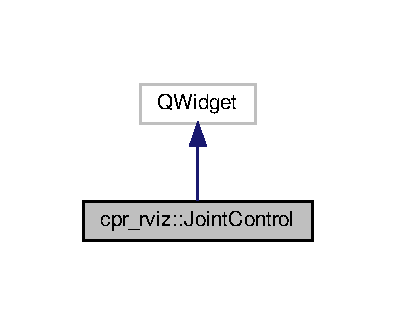
\includegraphics[width=190pt]{classcpr__rviz_1_1JointControl__inherit__graph}
\end{center}
\end{figure}
\subsection*{Public Member Functions}
\begin{DoxyCompactItemize}
\item 
void \textbf{ Disable} ()
\begin{DoxyCompactList}\small\item\em Disables all relevant UI elements. \end{DoxyCompactList}\item 
void \textbf{ Enable} ()
\begin{DoxyCompactList}\small\item\em Enables all relevant UI elements. \end{DoxyCompactList}\item 
bool \textbf{ get\+\_\+\+Referenced} () const
\begin{DoxyCompactList}\small\item\em Gets the referencing state. \end{DoxyCompactList}\item 
\textbf{ Joint\+Control} (const uint32\+\_\+t joint\+Id, Q\+Widget $\ast$parent=nullptr)
\begin{DoxyCompactList}\small\item\em Constructs a \doxyref{Joint\+Control}{p.}{classcpr__rviz_1_1JointControl} widget. \end{DoxyCompactList}\item 
void \textbf{ set\+\_\+\+Is\+Referenced} (const bool b\+Referenced)
\begin{DoxyCompactList}\small\item\em Sets the referencing state. \end{DoxyCompactList}\end{DoxyCompactItemize}
\subsection*{Protected Slots}
\begin{DoxyCompactItemize}
\item 
void \textbf{ On\+Stop\+Button\+Clicked} (bool checked=false)
\begin{DoxyCompactList}\small\item\em Callback slot that is called when the S\+T\+OP button is clicked. \end{DoxyCompactList}\item 
void \textbf{ On\+Velocity\+Slider\+Value\+Changed} (int value)
\begin{DoxyCompactList}\small\item\em Callback slot that handles changes to the velocity control slider. \end{DoxyCompactList}\end{DoxyCompactItemize}
\subsection*{Protected Member Functions}
\begin{DoxyCompactItemize}
\item 
cpr\+\_\+robot\+::\+Get\+Joint\+Info\+Response \textbf{ Get\+Joint\+Info} ()
\begin{DoxyCompactList}\small\item\em Queries information about the joint from the /\+Get\+Joint\+Info R\+OS service. \end{DoxyCompactList}\end{DoxyCompactItemize}
\subsection*{Private Member Functions}
\begin{DoxyCompactItemize}
\item 
void \textbf{ Initialize\+R\+OS} ()
\begin{DoxyCompactList}\small\item\em Sets up communication with R\+OS. \end{DoxyCompactList}\item 
void \textbf{ Initialize\+State} ()
\begin{DoxyCompactList}\small\item\em Initializes all relevant members. \end{DoxyCompactList}\item 
void \textbf{ Initialize\+UI} ()
\begin{DoxyCompactList}\small\item\em Initializes all UI elements. \end{DoxyCompactList}\item 
void \textbf{ Joint\+State\+Callback} (const sensor\+\_\+msgs\+::\+Joint\+State\+::\+Const\+Ptr \&msg)
\begin{DoxyCompactList}\small\item\em Callback that handles messages received over the /\+Joint\+State R\+OS topic. \end{DoxyCompactList}\item 
void \textbf{ On\+Position\+Changed} ()
\begin{DoxyCompactList}\small\item\em Updates the UI elements associated with position. \end{DoxyCompactList}\item 
void \textbf{ On\+Velocity\+Changed} ()
\begin{DoxyCompactList}\small\item\em Updates the UI elements associated with velocity. \end{DoxyCompactList}\end{DoxyCompactItemize}
\subsection*{Private Attributes}
\begin{DoxyCompactItemize}
\item 
bool \textbf{ m\+\_\+b\+Is\+Referenced}
\begin{DoxyCompactList}\small\item\em Flag indicating whether the joint has been referenced. \end{DoxyCompactList}\item 
ros\+::\+Service\+Client \textbf{ m\+\_\+\+Get\+Joint\+Info\+Client}
\begin{DoxyCompactList}\small\item\em Client used to query information about the joint via the /\+Get\+Joint\+Info R\+OS service. \end{DoxyCompactList}\item 
Q\+Group\+Box \textbf{ m\+\_\+\+Group\+Box}
\begin{DoxyCompactList}\small\item\em A group box widget that will contain the controls. \end{DoxyCompactList}\item 
Q\+Form\+Layout \textbf{ m\+\_\+\+Group\+Layout}
\begin{DoxyCompactList}\small\item\em The layout arranging the controls in the group box. \end{DoxyCompactList}\item 
uint32\+\_\+t \textbf{ m\+\_\+\+Joint\+Id}
\begin{DoxyCompactList}\small\item\em The ID of the joint. \end{DoxyCompactList}\item 
ros\+::\+Publisher \textbf{ m\+\_\+\+Joint\+Jog\+Publisher}
\begin{DoxyCompactList}\small\item\em Publisher used to publish jog commands over the /\+Joint\+Jog R\+OS topic. \end{DoxyCompactList}\item 
std\+::string \textbf{ m\+\_\+\+Joint\+Name}
\begin{DoxyCompactList}\small\item\em The name of the joint as used in R\+OS topics and services. \end{DoxyCompactList}\item 
ros\+::\+Subscriber \textbf{ m\+\_\+\+Joint\+State\+Subscriber}
\begin{DoxyCompactList}\small\item\em Subscriber that will listen for joint states on the /joint\+\_\+states R\+OS topic. \end{DoxyCompactList}\item 
uint32\+\_\+t \textbf{ m\+\_\+\+Joint\+Type}
\begin{DoxyCompactList}\small\item\em The joint type. Currently this is not used. \end{DoxyCompactList}\item 
Q\+H\+Box\+Layout \textbf{ m\+\_\+\+Main\+Layout}
\begin{DoxyCompactList}\small\item\em The top-\/level layout of the widget. \end{DoxyCompactList}\item 
ros\+::\+Node\+Handle \textbf{ m\+\_\+\+Node}
\begin{DoxyCompactList}\small\item\em A handle to the current R\+OS node. \end{DoxyCompactList}\item 
double \textbf{ m\+\_\+\+Position}
\begin{DoxyCompactList}\small\item\em The position of the joint in radians. \end{DoxyCompactList}\item 
Q\+Label \textbf{ m\+\_\+\+Position\+Label}
\begin{DoxyCompactList}\small\item\em A label that will show the current position. \end{DoxyCompactList}\item 
Q\+Push\+Button \textbf{ m\+\_\+\+Stop\+Button}
\begin{DoxyCompactList}\small\item\em A button that will set the desired velocity to zero when pressed. \end{DoxyCompactList}\item 
double \textbf{ m\+\_\+\+Velocity}
\begin{DoxyCompactList}\small\item\em The angular velocity of the joint in radians per second. \end{DoxyCompactList}\item 
Q\+Label \textbf{ m\+\_\+\+Velocity\+Label}
\begin{DoxyCompactList}\small\item\em A label that will show the current velocity. \end{DoxyCompactList}\item 
Q\+Slider \textbf{ m\+\_\+\+Velocity\+Slider}
\begin{DoxyCompactList}\small\item\em A slider that allows to control the desired velocity. \end{DoxyCompactList}\end{DoxyCompactItemize}


\subsection{Detailed Description}
Widget that provides motion control for a single robot joint. 

Definition at line 7 of file Joint\+Control.\+h.



\subsection{Constructor \& Destructor Documentation}
\mbox{\label{classcpr__rviz_1_1JointControl_a3c0564180d0abaaf761d993b744ce29b}} 
\index{cpr\+\_\+rviz\+::\+Joint\+Control@{cpr\+\_\+rviz\+::\+Joint\+Control}!Joint\+Control@{Joint\+Control}}
\index{Joint\+Control@{Joint\+Control}!cpr\+\_\+rviz\+::\+Joint\+Control@{cpr\+\_\+rviz\+::\+Joint\+Control}}
\subsubsection{Joint\+Control()}
{\footnotesize\ttfamily cpr\+\_\+rviz\+::\+Joint\+Control\+::\+Joint\+Control (\begin{DoxyParamCaption}\item[{const uint32\+\_\+t}]{joint\+Id,  }\item[{Q\+Widget $\ast$}]{parent = {\ttfamily nullptr} }\end{DoxyParamCaption})}



Constructs a \doxyref{Joint\+Control}{p.}{classcpr__rviz_1_1JointControl} widget. 


\begin{DoxyParams}{Parameters}
{\em joint\+Id} & The ID of the joint that will be controlled by the widget. \\
\hline
{\em parent} & The parent widget \\
\hline
\end{DoxyParams}


Definition at line 12 of file Joint\+Control.\+cpp.



\subsection{Member Function Documentation}
\mbox{\label{classcpr__rviz_1_1JointControl_a8a3333b09fe8987e3fe1964d97500389}} 
\index{cpr\+\_\+rviz\+::\+Joint\+Control@{cpr\+\_\+rviz\+::\+Joint\+Control}!Disable@{Disable}}
\index{Disable@{Disable}!cpr\+\_\+rviz\+::\+Joint\+Control@{cpr\+\_\+rviz\+::\+Joint\+Control}}
\subsubsection{Disable()}
{\footnotesize\ttfamily void cpr\+\_\+rviz\+::\+Joint\+Control\+::\+Disable (\begin{DoxyParamCaption}{ }\end{DoxyParamCaption})}



Disables all relevant UI elements. 



Definition at line 76 of file Joint\+Control.\+cpp.

\mbox{\label{classcpr__rviz_1_1JointControl_af043fa940778ae0875347c0c6e924673}} 
\index{cpr\+\_\+rviz\+::\+Joint\+Control@{cpr\+\_\+rviz\+::\+Joint\+Control}!Enable@{Enable}}
\index{Enable@{Enable}!cpr\+\_\+rviz\+::\+Joint\+Control@{cpr\+\_\+rviz\+::\+Joint\+Control}}
\subsubsection{Enable()}
{\footnotesize\ttfamily void cpr\+\_\+rviz\+::\+Joint\+Control\+::\+Enable (\begin{DoxyParamCaption}{ }\end{DoxyParamCaption})}



Enables all relevant UI elements. 



Definition at line 68 of file Joint\+Control.\+cpp.

\mbox{\label{classcpr__rviz_1_1JointControl_a075915255bca76fc81c6b761d08417ad}} 
\index{cpr\+\_\+rviz\+::\+Joint\+Control@{cpr\+\_\+rviz\+::\+Joint\+Control}!get\+\_\+\+Referenced@{get\+\_\+\+Referenced}}
\index{get\+\_\+\+Referenced@{get\+\_\+\+Referenced}!cpr\+\_\+rviz\+::\+Joint\+Control@{cpr\+\_\+rviz\+::\+Joint\+Control}}
\subsubsection{get\+\_\+\+Referenced()}
{\footnotesize\ttfamily bool cpr\+\_\+rviz\+::\+Joint\+Control\+::get\+\_\+\+Referenced (\begin{DoxyParamCaption}{ }\end{DoxyParamCaption}) const}



Gets the referencing state. 

\begin{DoxyReturn}{Returns}
Flag indicating whether the joint has been referenced. 
\end{DoxyReturn}


Definition at line 62 of file Joint\+Control.\+cpp.

\mbox{\label{classcpr__rviz_1_1JointControl_a1d5ed10095d9f18c3895db5083d8e754}} 
\index{cpr\+\_\+rviz\+::\+Joint\+Control@{cpr\+\_\+rviz\+::\+Joint\+Control}!Get\+Joint\+Info@{Get\+Joint\+Info}}
\index{Get\+Joint\+Info@{Get\+Joint\+Info}!cpr\+\_\+rviz\+::\+Joint\+Control@{cpr\+\_\+rviz\+::\+Joint\+Control}}
\subsubsection{Get\+Joint\+Info()}
{\footnotesize\ttfamily cpr\+\_\+robot\+::\+Get\+Joint\+Info\+Response cpr\+\_\+rviz\+::\+Joint\+Control\+::\+Get\+Joint\+Info (\begin{DoxyParamCaption}{ }\end{DoxyParamCaption})\hspace{0.3cm}{\ttfamily [protected]}}



Queries information about the joint from the /\+Get\+Joint\+Info R\+OS service. 



Definition at line 161 of file Joint\+Control.\+cpp.

\mbox{\label{classcpr__rviz_1_1JointControl_a38be0ce51423a08696490a30fb002091}} 
\index{cpr\+\_\+rviz\+::\+Joint\+Control@{cpr\+\_\+rviz\+::\+Joint\+Control}!Initialize\+R\+OS@{Initialize\+R\+OS}}
\index{Initialize\+R\+OS@{Initialize\+R\+OS}!cpr\+\_\+rviz\+::\+Joint\+Control@{cpr\+\_\+rviz\+::\+Joint\+Control}}
\subsubsection{Initialize\+R\+O\+S()}
{\footnotesize\ttfamily void cpr\+\_\+rviz\+::\+Joint\+Control\+::\+Initialize\+R\+OS (\begin{DoxyParamCaption}{ }\end{DoxyParamCaption})\hspace{0.3cm}{\ttfamily [private]}}



Sets up communication with R\+OS. 



Definition at line 118 of file Joint\+Control.\+cpp.

\mbox{\label{classcpr__rviz_1_1JointControl_ae6ba57f3056fa550aa0a4258266c150c}} 
\index{cpr\+\_\+rviz\+::\+Joint\+Control@{cpr\+\_\+rviz\+::\+Joint\+Control}!Initialize\+State@{Initialize\+State}}
\index{Initialize\+State@{Initialize\+State}!cpr\+\_\+rviz\+::\+Joint\+Control@{cpr\+\_\+rviz\+::\+Joint\+Control}}
\subsubsection{Initialize\+State()}
{\footnotesize\ttfamily void cpr\+\_\+rviz\+::\+Joint\+Control\+::\+Initialize\+State (\begin{DoxyParamCaption}{ }\end{DoxyParamCaption})\hspace{0.3cm}{\ttfamily [private]}}



Initializes all relevant members. 



Definition at line 108 of file Joint\+Control.\+cpp.

\mbox{\label{classcpr__rviz_1_1JointControl_a6c87f4bf2a1df5d7d8f0494bf27a163b}} 
\index{cpr\+\_\+rviz\+::\+Joint\+Control@{cpr\+\_\+rviz\+::\+Joint\+Control}!Initialize\+UI@{Initialize\+UI}}
\index{Initialize\+UI@{Initialize\+UI}!cpr\+\_\+rviz\+::\+Joint\+Control@{cpr\+\_\+rviz\+::\+Joint\+Control}}
\subsubsection{Initialize\+U\+I()}
{\footnotesize\ttfamily void cpr\+\_\+rviz\+::\+Joint\+Control\+::\+Initialize\+UI (\begin{DoxyParamCaption}{ }\end{DoxyParamCaption})\hspace{0.3cm}{\ttfamily [private]}}



Initializes all UI elements. 



Definition at line 27 of file Joint\+Control.\+cpp.

\mbox{\label{classcpr__rviz_1_1JointControl_a9938dd5fb01d40daea1ccdda0062d157}} 
\index{cpr\+\_\+rviz\+::\+Joint\+Control@{cpr\+\_\+rviz\+::\+Joint\+Control}!Joint\+State\+Callback@{Joint\+State\+Callback}}
\index{Joint\+State\+Callback@{Joint\+State\+Callback}!cpr\+\_\+rviz\+::\+Joint\+Control@{cpr\+\_\+rviz\+::\+Joint\+Control}}
\subsubsection{Joint\+State\+Callback()}
{\footnotesize\ttfamily void cpr\+\_\+rviz\+::\+Joint\+Control\+::\+Joint\+State\+Callback (\begin{DoxyParamCaption}\item[{const sensor\+\_\+msgs\+::\+Joint\+State\+::\+Const\+Ptr \&}]{msg }\end{DoxyParamCaption})\hspace{0.3cm}{\ttfamily [private]}}



Callback that handles messages received over the /\+Joint\+State R\+OS topic. 


\begin{DoxyParams}{Parameters}
{\em msg} & The received message. \\
\hline
\end{DoxyParams}


Definition at line 127 of file Joint\+Control.\+cpp.

\mbox{\label{classcpr__rviz_1_1JointControl_a1816ea27f1f667c9c8d4a796afd42cf2}} 
\index{cpr\+\_\+rviz\+::\+Joint\+Control@{cpr\+\_\+rviz\+::\+Joint\+Control}!On\+Position\+Changed@{On\+Position\+Changed}}
\index{On\+Position\+Changed@{On\+Position\+Changed}!cpr\+\_\+rviz\+::\+Joint\+Control@{cpr\+\_\+rviz\+::\+Joint\+Control}}
\subsubsection{On\+Position\+Changed()}
{\footnotesize\ttfamily void cpr\+\_\+rviz\+::\+Joint\+Control\+::\+On\+Position\+Changed (\begin{DoxyParamCaption}{ }\end{DoxyParamCaption})\hspace{0.3cm}{\ttfamily [private]}}



Updates the UI elements associated with position. 



Definition at line 98 of file Joint\+Control.\+cpp.

\mbox{\label{classcpr__rviz_1_1JointControl_a941d660f63009403405df8f13aaf989b}} 
\index{cpr\+\_\+rviz\+::\+Joint\+Control@{cpr\+\_\+rviz\+::\+Joint\+Control}!On\+Stop\+Button\+Clicked@{On\+Stop\+Button\+Clicked}}
\index{On\+Stop\+Button\+Clicked@{On\+Stop\+Button\+Clicked}!cpr\+\_\+rviz\+::\+Joint\+Control@{cpr\+\_\+rviz\+::\+Joint\+Control}}
\subsubsection{On\+Stop\+Button\+Clicked}
{\footnotesize\ttfamily void cpr\+\_\+rviz\+::\+Joint\+Control\+::\+On\+Stop\+Button\+Clicked (\begin{DoxyParamCaption}\item[{bool}]{checked = {\ttfamily false} }\end{DoxyParamCaption})\hspace{0.3cm}{\ttfamily [protected]}, {\ttfamily [slot]}}



Callback slot that is called when the S\+T\+OP button is clicked. 



Definition at line 84 of file Joint\+Control.\+cpp.

\mbox{\label{classcpr__rviz_1_1JointControl_a208e7c277741ff60c9f735cf602eb36c}} 
\index{cpr\+\_\+rviz\+::\+Joint\+Control@{cpr\+\_\+rviz\+::\+Joint\+Control}!On\+Velocity\+Changed@{On\+Velocity\+Changed}}
\index{On\+Velocity\+Changed@{On\+Velocity\+Changed}!cpr\+\_\+rviz\+::\+Joint\+Control@{cpr\+\_\+rviz\+::\+Joint\+Control}}
\subsubsection{On\+Velocity\+Changed()}
{\footnotesize\ttfamily void cpr\+\_\+rviz\+::\+Joint\+Control\+::\+On\+Velocity\+Changed (\begin{DoxyParamCaption}{ }\end{DoxyParamCaption})\hspace{0.3cm}{\ttfamily [private]}}



Updates the UI elements associated with velocity. 



Definition at line 90 of file Joint\+Control.\+cpp.

\mbox{\label{classcpr__rviz_1_1JointControl_a413b023c830fd1d723bab917973bc3f3}} 
\index{cpr\+\_\+rviz\+::\+Joint\+Control@{cpr\+\_\+rviz\+::\+Joint\+Control}!On\+Velocity\+Slider\+Value\+Changed@{On\+Velocity\+Slider\+Value\+Changed}}
\index{On\+Velocity\+Slider\+Value\+Changed@{On\+Velocity\+Slider\+Value\+Changed}!cpr\+\_\+rviz\+::\+Joint\+Control@{cpr\+\_\+rviz\+::\+Joint\+Control}}
\subsubsection{On\+Velocity\+Slider\+Value\+Changed}
{\footnotesize\ttfamily void cpr\+\_\+rviz\+::\+Joint\+Control\+::\+On\+Velocity\+Slider\+Value\+Changed (\begin{DoxyParamCaption}\item[{int}]{value }\end{DoxyParamCaption})\hspace{0.3cm}{\ttfamily [protected]}, {\ttfamily [slot]}}



Callback slot that handles changes to the velocity control slider. 



Definition at line 150 of file Joint\+Control.\+cpp.

\mbox{\label{classcpr__rviz_1_1JointControl_a2f5454e18d7d23e944395ada7aaeba36}} 
\index{cpr\+\_\+rviz\+::\+Joint\+Control@{cpr\+\_\+rviz\+::\+Joint\+Control}!set\+\_\+\+Is\+Referenced@{set\+\_\+\+Is\+Referenced}}
\index{set\+\_\+\+Is\+Referenced@{set\+\_\+\+Is\+Referenced}!cpr\+\_\+rviz\+::\+Joint\+Control@{cpr\+\_\+rviz\+::\+Joint\+Control}}
\subsubsection{set\+\_\+\+Is\+Referenced()}
{\footnotesize\ttfamily void cpr\+\_\+rviz\+::\+Joint\+Control\+::set\+\_\+\+Is\+Referenced (\begin{DoxyParamCaption}\item[{const bool}]{b\+Referenced }\end{DoxyParamCaption})}



Sets the referencing state. 


\begin{DoxyParams}{Parameters}
{\em b\+Referenced} & Flag indicating whether the joint has been referenced. \\
\hline
\end{DoxyParams}


Definition at line 51 of file Joint\+Control.\+cpp.



\subsection{Member Data Documentation}
\mbox{\label{classcpr__rviz_1_1JointControl_ae93ea47479c5a1d93edccddb1653c045}} 
\index{cpr\+\_\+rviz\+::\+Joint\+Control@{cpr\+\_\+rviz\+::\+Joint\+Control}!m\+\_\+b\+Is\+Referenced@{m\+\_\+b\+Is\+Referenced}}
\index{m\+\_\+b\+Is\+Referenced@{m\+\_\+b\+Is\+Referenced}!cpr\+\_\+rviz\+::\+Joint\+Control@{cpr\+\_\+rviz\+::\+Joint\+Control}}
\subsubsection{m\+\_\+b\+Is\+Referenced}
{\footnotesize\ttfamily bool cpr\+\_\+rviz\+::\+Joint\+Control\+::m\+\_\+b\+Is\+Referenced\hspace{0.3cm}{\ttfamily [private]}}



Flag indicating whether the joint has been referenced. 



Definition at line 28 of file Joint\+Control.\+h.

\mbox{\label{classcpr__rviz_1_1JointControl_a6a62524861cf3adc8d2d80b35d62371b}} 
\index{cpr\+\_\+rviz\+::\+Joint\+Control@{cpr\+\_\+rviz\+::\+Joint\+Control}!m\+\_\+\+Get\+Joint\+Info\+Client@{m\+\_\+\+Get\+Joint\+Info\+Client}}
\index{m\+\_\+\+Get\+Joint\+Info\+Client@{m\+\_\+\+Get\+Joint\+Info\+Client}!cpr\+\_\+rviz\+::\+Joint\+Control@{cpr\+\_\+rviz\+::\+Joint\+Control}}
\subsubsection{m\+\_\+\+Get\+Joint\+Info\+Client}
{\footnotesize\ttfamily ros\+::\+Service\+Client cpr\+\_\+rviz\+::\+Joint\+Control\+::m\+\_\+\+Get\+Joint\+Info\+Client\hspace{0.3cm}{\ttfamily [private]}}



Client used to query information about the joint via the /\+Get\+Joint\+Info R\+OS service. 



Definition at line 14 of file Joint\+Control.\+h.

\mbox{\label{classcpr__rviz_1_1JointControl_afc8b3eff7c725da9894dd3bddd3e6f86}} 
\index{cpr\+\_\+rviz\+::\+Joint\+Control@{cpr\+\_\+rviz\+::\+Joint\+Control}!m\+\_\+\+Group\+Box@{m\+\_\+\+Group\+Box}}
\index{m\+\_\+\+Group\+Box@{m\+\_\+\+Group\+Box}!cpr\+\_\+rviz\+::\+Joint\+Control@{cpr\+\_\+rviz\+::\+Joint\+Control}}
\subsubsection{m\+\_\+\+Group\+Box}
{\footnotesize\ttfamily Q\+Group\+Box cpr\+\_\+rviz\+::\+Joint\+Control\+::m\+\_\+\+Group\+Box\hspace{0.3cm}{\ttfamily [private]}}



A group box widget that will contain the controls. 



Definition at line 34 of file Joint\+Control.\+h.

\mbox{\label{classcpr__rviz_1_1JointControl_afb27353b7d3325bf8744f2e98b91bbe5}} 
\index{cpr\+\_\+rviz\+::\+Joint\+Control@{cpr\+\_\+rviz\+::\+Joint\+Control}!m\+\_\+\+Group\+Layout@{m\+\_\+\+Group\+Layout}}
\index{m\+\_\+\+Group\+Layout@{m\+\_\+\+Group\+Layout}!cpr\+\_\+rviz\+::\+Joint\+Control@{cpr\+\_\+rviz\+::\+Joint\+Control}}
\subsubsection{m\+\_\+\+Group\+Layout}
{\footnotesize\ttfamily Q\+Form\+Layout cpr\+\_\+rviz\+::\+Joint\+Control\+::m\+\_\+\+Group\+Layout\hspace{0.3cm}{\ttfamily [private]}}



The layout arranging the controls in the group box. 



Definition at line 36 of file Joint\+Control.\+h.

\mbox{\label{classcpr__rviz_1_1JointControl_a61275106767d7070097f9b75af1bc9d4}} 
\index{cpr\+\_\+rviz\+::\+Joint\+Control@{cpr\+\_\+rviz\+::\+Joint\+Control}!m\+\_\+\+Joint\+Id@{m\+\_\+\+Joint\+Id}}
\index{m\+\_\+\+Joint\+Id@{m\+\_\+\+Joint\+Id}!cpr\+\_\+rviz\+::\+Joint\+Control@{cpr\+\_\+rviz\+::\+Joint\+Control}}
\subsubsection{m\+\_\+\+Joint\+Id}
{\footnotesize\ttfamily uint32\+\_\+t cpr\+\_\+rviz\+::\+Joint\+Control\+::m\+\_\+\+Joint\+Id\hspace{0.3cm}{\ttfamily [private]}}



The ID of the joint. 



Definition at line 20 of file Joint\+Control.\+h.

\mbox{\label{classcpr__rviz_1_1JointControl_afa91714093241494d20a3d0749cc99be}} 
\index{cpr\+\_\+rviz\+::\+Joint\+Control@{cpr\+\_\+rviz\+::\+Joint\+Control}!m\+\_\+\+Joint\+Jog\+Publisher@{m\+\_\+\+Joint\+Jog\+Publisher}}
\index{m\+\_\+\+Joint\+Jog\+Publisher@{m\+\_\+\+Joint\+Jog\+Publisher}!cpr\+\_\+rviz\+::\+Joint\+Control@{cpr\+\_\+rviz\+::\+Joint\+Control}}
\subsubsection{m\+\_\+\+Joint\+Jog\+Publisher}
{\footnotesize\ttfamily ros\+::\+Publisher cpr\+\_\+rviz\+::\+Joint\+Control\+::m\+\_\+\+Joint\+Jog\+Publisher\hspace{0.3cm}{\ttfamily [private]}}



Publisher used to publish jog commands over the /\+Joint\+Jog R\+OS topic. 



Definition at line 16 of file Joint\+Control.\+h.

\mbox{\label{classcpr__rviz_1_1JointControl_a2aec12d818ded0a8bedfb93ffd3ded32}} 
\index{cpr\+\_\+rviz\+::\+Joint\+Control@{cpr\+\_\+rviz\+::\+Joint\+Control}!m\+\_\+\+Joint\+Name@{m\+\_\+\+Joint\+Name}}
\index{m\+\_\+\+Joint\+Name@{m\+\_\+\+Joint\+Name}!cpr\+\_\+rviz\+::\+Joint\+Control@{cpr\+\_\+rviz\+::\+Joint\+Control}}
\subsubsection{m\+\_\+\+Joint\+Name}
{\footnotesize\ttfamily std\+::string cpr\+\_\+rviz\+::\+Joint\+Control\+::m\+\_\+\+Joint\+Name\hspace{0.3cm}{\ttfamily [private]}}



The name of the joint as used in R\+OS topics and services. 



Definition at line 22 of file Joint\+Control.\+h.

\mbox{\label{classcpr__rviz_1_1JointControl_a6e1364b45555ee1aef13efe5ae41a62b}} 
\index{cpr\+\_\+rviz\+::\+Joint\+Control@{cpr\+\_\+rviz\+::\+Joint\+Control}!m\+\_\+\+Joint\+State\+Subscriber@{m\+\_\+\+Joint\+State\+Subscriber}}
\index{m\+\_\+\+Joint\+State\+Subscriber@{m\+\_\+\+Joint\+State\+Subscriber}!cpr\+\_\+rviz\+::\+Joint\+Control@{cpr\+\_\+rviz\+::\+Joint\+Control}}
\subsubsection{m\+\_\+\+Joint\+State\+Subscriber}
{\footnotesize\ttfamily ros\+::\+Subscriber cpr\+\_\+rviz\+::\+Joint\+Control\+::m\+\_\+\+Joint\+State\+Subscriber\hspace{0.3cm}{\ttfamily [private]}}



Subscriber that will listen for joint states on the /joint\+\_\+states R\+OS topic. 



Definition at line 18 of file Joint\+Control.\+h.

\mbox{\label{classcpr__rviz_1_1JointControl_a5df1b323959812671f46b685e44a4c23}} 
\index{cpr\+\_\+rviz\+::\+Joint\+Control@{cpr\+\_\+rviz\+::\+Joint\+Control}!m\+\_\+\+Joint\+Type@{m\+\_\+\+Joint\+Type}}
\index{m\+\_\+\+Joint\+Type@{m\+\_\+\+Joint\+Type}!cpr\+\_\+rviz\+::\+Joint\+Control@{cpr\+\_\+rviz\+::\+Joint\+Control}}
\subsubsection{m\+\_\+\+Joint\+Type}
{\footnotesize\ttfamily uint32\+\_\+t cpr\+\_\+rviz\+::\+Joint\+Control\+::m\+\_\+\+Joint\+Type\hspace{0.3cm}{\ttfamily [private]}}



The joint type. Currently this is not used. 



Definition at line 30 of file Joint\+Control.\+h.

\mbox{\label{classcpr__rviz_1_1JointControl_a2d6645a68741014a1fee4525c169933d}} 
\index{cpr\+\_\+rviz\+::\+Joint\+Control@{cpr\+\_\+rviz\+::\+Joint\+Control}!m\+\_\+\+Main\+Layout@{m\+\_\+\+Main\+Layout}}
\index{m\+\_\+\+Main\+Layout@{m\+\_\+\+Main\+Layout}!cpr\+\_\+rviz\+::\+Joint\+Control@{cpr\+\_\+rviz\+::\+Joint\+Control}}
\subsubsection{m\+\_\+\+Main\+Layout}
{\footnotesize\ttfamily Q\+H\+Box\+Layout cpr\+\_\+rviz\+::\+Joint\+Control\+::m\+\_\+\+Main\+Layout\hspace{0.3cm}{\ttfamily [private]}}



The top-\/level layout of the widget. 



Definition at line 32 of file Joint\+Control.\+h.

\mbox{\label{classcpr__rviz_1_1JointControl_ac0c9e57f9aa2fdf990e012f3c6194ae6}} 
\index{cpr\+\_\+rviz\+::\+Joint\+Control@{cpr\+\_\+rviz\+::\+Joint\+Control}!m\+\_\+\+Node@{m\+\_\+\+Node}}
\index{m\+\_\+\+Node@{m\+\_\+\+Node}!cpr\+\_\+rviz\+::\+Joint\+Control@{cpr\+\_\+rviz\+::\+Joint\+Control}}
\subsubsection{m\+\_\+\+Node}
{\footnotesize\ttfamily ros\+::\+Node\+Handle cpr\+\_\+rviz\+::\+Joint\+Control\+::m\+\_\+\+Node\hspace{0.3cm}{\ttfamily [private]}}



A handle to the current R\+OS node. 



Definition at line 12 of file Joint\+Control.\+h.

\mbox{\label{classcpr__rviz_1_1JointControl_aaba2872c9325724d919cedf24c785581}} 
\index{cpr\+\_\+rviz\+::\+Joint\+Control@{cpr\+\_\+rviz\+::\+Joint\+Control}!m\+\_\+\+Position@{m\+\_\+\+Position}}
\index{m\+\_\+\+Position@{m\+\_\+\+Position}!cpr\+\_\+rviz\+::\+Joint\+Control@{cpr\+\_\+rviz\+::\+Joint\+Control}}
\subsubsection{m\+\_\+\+Position}
{\footnotesize\ttfamily double cpr\+\_\+rviz\+::\+Joint\+Control\+::m\+\_\+\+Position\hspace{0.3cm}{\ttfamily [private]}}



The position of the joint in radians. 



Definition at line 24 of file Joint\+Control.\+h.

\mbox{\label{classcpr__rviz_1_1JointControl_aa8a7ae5e85dbc6656d4d68ad2317ec6d}} 
\index{cpr\+\_\+rviz\+::\+Joint\+Control@{cpr\+\_\+rviz\+::\+Joint\+Control}!m\+\_\+\+Position\+Label@{m\+\_\+\+Position\+Label}}
\index{m\+\_\+\+Position\+Label@{m\+\_\+\+Position\+Label}!cpr\+\_\+rviz\+::\+Joint\+Control@{cpr\+\_\+rviz\+::\+Joint\+Control}}
\subsubsection{m\+\_\+\+Position\+Label}
{\footnotesize\ttfamily Q\+Label cpr\+\_\+rviz\+::\+Joint\+Control\+::m\+\_\+\+Position\+Label\hspace{0.3cm}{\ttfamily [private]}}



A label that will show the current position. 



Definition at line 38 of file Joint\+Control.\+h.

\mbox{\label{classcpr__rviz_1_1JointControl_a05dabe23a265d5a9b2220ef037d2ac4e}} 
\index{cpr\+\_\+rviz\+::\+Joint\+Control@{cpr\+\_\+rviz\+::\+Joint\+Control}!m\+\_\+\+Stop\+Button@{m\+\_\+\+Stop\+Button}}
\index{m\+\_\+\+Stop\+Button@{m\+\_\+\+Stop\+Button}!cpr\+\_\+rviz\+::\+Joint\+Control@{cpr\+\_\+rviz\+::\+Joint\+Control}}
\subsubsection{m\+\_\+\+Stop\+Button}
{\footnotesize\ttfamily Q\+Push\+Button cpr\+\_\+rviz\+::\+Joint\+Control\+::m\+\_\+\+Stop\+Button\hspace{0.3cm}{\ttfamily [private]}}



A button that will set the desired velocity to zero when pressed. 



Definition at line 44 of file Joint\+Control.\+h.

\mbox{\label{classcpr__rviz_1_1JointControl_a7286a9251862f81863d4dc800f565d4e}} 
\index{cpr\+\_\+rviz\+::\+Joint\+Control@{cpr\+\_\+rviz\+::\+Joint\+Control}!m\+\_\+\+Velocity@{m\+\_\+\+Velocity}}
\index{m\+\_\+\+Velocity@{m\+\_\+\+Velocity}!cpr\+\_\+rviz\+::\+Joint\+Control@{cpr\+\_\+rviz\+::\+Joint\+Control}}
\subsubsection{m\+\_\+\+Velocity}
{\footnotesize\ttfamily double cpr\+\_\+rviz\+::\+Joint\+Control\+::m\+\_\+\+Velocity\hspace{0.3cm}{\ttfamily [private]}}



The angular velocity of the joint in radians per second. 



Definition at line 26 of file Joint\+Control.\+h.

\mbox{\label{classcpr__rviz_1_1JointControl_ab5e1719b2b756adcf099f03dd7aa2361}} 
\index{cpr\+\_\+rviz\+::\+Joint\+Control@{cpr\+\_\+rviz\+::\+Joint\+Control}!m\+\_\+\+Velocity\+Label@{m\+\_\+\+Velocity\+Label}}
\index{m\+\_\+\+Velocity\+Label@{m\+\_\+\+Velocity\+Label}!cpr\+\_\+rviz\+::\+Joint\+Control@{cpr\+\_\+rviz\+::\+Joint\+Control}}
\subsubsection{m\+\_\+\+Velocity\+Label}
{\footnotesize\ttfamily Q\+Label cpr\+\_\+rviz\+::\+Joint\+Control\+::m\+\_\+\+Velocity\+Label\hspace{0.3cm}{\ttfamily [private]}}



A label that will show the current velocity. 



Definition at line 40 of file Joint\+Control.\+h.

\mbox{\label{classcpr__rviz_1_1JointControl_a69fc8b3462fb5c62dd64119384e6aa7f}} 
\index{cpr\+\_\+rviz\+::\+Joint\+Control@{cpr\+\_\+rviz\+::\+Joint\+Control}!m\+\_\+\+Velocity\+Slider@{m\+\_\+\+Velocity\+Slider}}
\index{m\+\_\+\+Velocity\+Slider@{m\+\_\+\+Velocity\+Slider}!cpr\+\_\+rviz\+::\+Joint\+Control@{cpr\+\_\+rviz\+::\+Joint\+Control}}
\subsubsection{m\+\_\+\+Velocity\+Slider}
{\footnotesize\ttfamily Q\+Slider cpr\+\_\+rviz\+::\+Joint\+Control\+::m\+\_\+\+Velocity\+Slider\hspace{0.3cm}{\ttfamily [private]}}



A slider that allows to control the desired velocity. 



Definition at line 42 of file Joint\+Control.\+h.



The documentation for this class was generated from the following files\+:\begin{DoxyCompactItemize}
\item 
\textbf{ Joint\+Control.\+h}\item 
\textbf{ Joint\+Control.\+cpp}\end{DoxyCompactItemize}

\section{cpr\+\_\+robot\+:\+:Motor\+Module Class Reference}
\label{classcpr__robot_1_1MotorModule}\index{cpr\+\_\+robot\+::\+Motor\+Module@{cpr\+\_\+robot\+::\+Motor\+Module}}


Represents a D\+IN rail motorcontrol module from Commonplace Robotics GmbH.  




{\ttfamily \#include $<$cpr\+\_\+robot.\+h$>$}

\subsection*{Public Member Functions}
\begin{DoxyCompactItemize}
\item 
void \textbf{ Disable} ()
\begin{DoxyCompactList}\small\item\em Disables motor motion. \end{DoxyCompactList}\item 
void \textbf{ Enable} ()
\begin{DoxyCompactList}\small\item\em Enables motor motion. \end{DoxyCompactList}\item 
int32\+\_\+t \textbf{ get\+\_\+\+Current\+Position} (uint8\+\_\+t \&time\+Stamp, std\+::chrono\+::high\+\_\+resolution\+\_\+clock\+::time\+\_\+point \&reception\+Time, uint8\+\_\+t \&error\+Flags, uint8\+\_\+t \&data\+Bits) const
\begin{DoxyCompactList}\small\item\em Allows to query the last response to a Set\+Joint command that has been received from the module. \end{DoxyCompactList}\item 
int32\+\_\+t \textbf{ get\+\_\+\+Desired\+Position} () const
\begin{DoxyCompactList}\small\item\em Allows to query the desired position of the joint that is controled by the D\+IN rail module. \end{DoxyCompactList}\item 
int32\+\_\+t \textbf{ get\+\_\+\+Increment} () const
\begin{DoxyCompactList}\small\item\em Gets the current encoder tick increment. \end{DoxyCompactList}\item 
int32\+\_\+t \textbf{ get\+\_\+\+Max\+Position} () const
\begin{DoxyCompactList}\small\item\em Gets the maximally allowed encoder position. \end{DoxyCompactList}\item 
int32\+\_\+t \textbf{ get\+\_\+\+Min\+Position} () const
\begin{DoxyCompactList}\small\item\em Gets the minimally allowed encoder position. \end{DoxyCompactList}\item 
uint8\+\_\+t \textbf{ get\+\_\+\+Module\+Id} () const
\begin{DoxyCompactList}\small\item\em Allows to query the ID of the D\+IN rail module. \end{DoxyCompactList}\item 
int32\+\_\+t \textbf{ get\+\_\+\+Offset} () const
\begin{DoxyCompactList}\small\item\em Gets the constant offset to be added to the motor position (\char`\"{}zero position\char`\"{}), measured in ticks. \end{DoxyCompactList}\item 
double \textbf{ get\+\_\+\+Update\+Interval} () const
\begin{DoxyCompactList}\small\item\em Gets the interval at which periodic Set\+Joint commands will be sent to the module in milliseconds. \end{DoxyCompactList}\item 
\textbf{ Motor\+Module} (\textbf{ Bus} \&canbus, const uint8\+\_\+t module\+Id)
\begin{DoxyCompactList}\small\item\em Constructor of the \doxyref{Motor\+Module}{p.}{classcpr__robot_1_1MotorModule} class. \end{DoxyCompactList}\item 
void \textbf{ set\+\_\+\+Desired\+Position} (const int32\+\_\+t ticks)
\begin{DoxyCompactList}\small\item\em Allows to set the desired position of the joint that is controled by the D\+IN rail module. \end{DoxyCompactList}\item 
void \textbf{ set\+\_\+\+Increment} (const int32\+\_\+t ticks)
\begin{DoxyCompactList}\small\item\em Sets the desired encoder tick increment. \end{DoxyCompactList}\item 
void \textbf{ set\+\_\+\+Max\+Position} (const int32\+\_\+t ticks)
\begin{DoxyCompactList}\small\item\em Sets the maximally allowed encoder position. \end{DoxyCompactList}\item 
void \textbf{ set\+\_\+\+Min\+Position} (const int32\+\_\+t ticks)
\begin{DoxyCompactList}\small\item\em Sets the minimally allowed encoder position. \end{DoxyCompactList}\item 
void \textbf{ set\+\_\+\+Offset} (const int32\+\_\+t ticks)
\begin{DoxyCompactList}\small\item\em Sets the constant offset to be added to the motor position (\char`\"{}zero position\char`\"{}), measured in ticks. \end{DoxyCompactList}\item 
void \textbf{ Set\+Zero} ()
\begin{DoxyCompactList}\small\item\em Sets the encoder position to zero. \end{DoxyCompactList}\item 
void \textbf{ Start} ()
\begin{DoxyCompactList}\small\item\em Starts the thread that is spinning in the write loop that sends periodic Set\+Joint commands to the module over the C\+AN bus. \end{DoxyCompactList}\item 
void \textbf{ Start\+Referencing} ()
\begin{DoxyCompactList}\small\item\em Starts the referencing procedure. \end{DoxyCompactList}\item 
void \textbf{ Stop} ()
\begin{DoxyCompactList}\small\item\em Terminates and joins the thread that is spinning in the write loop that sends periodic Set\+Joint commands to the module over the C\+AN bus. \end{DoxyCompactList}\item 
virtual \textbf{ $\sim$\+Motor\+Module} ()
\begin{DoxyCompactList}\small\item\em Destructor of the \doxyref{Motor\+Module}{p.}{classcpr__robot_1_1MotorModule} class. \end{DoxyCompactList}\end{DoxyCompactItemize}
\subsection*{Static Public Attributes}
\begin{DoxyCompactItemize}
\item 
static constexpr uint32\+\_\+t \textbf{ S\+T\+A\+T\+U\+S\+F\+L\+A\+G\+\_\+\+B\+R\+O\+W\+N\+\_\+\+O\+UT} = 0x00000001
\begin{DoxyCompactList}\small\item\em Error flag indicating that the microcontroller restarted after a brown out because the suppy voltage was too low or µC got stuck. \end{DoxyCompactList}\item 
static constexpr uint32\+\_\+t \textbf{ S\+T\+A\+T\+U\+S\+F\+L\+A\+G\+\_\+\+C\+A\+N\+\_\+\+E\+R\+R\+OR} = 0x00000080
\begin{DoxyCompactList}\small\item\em Error flag indicating that a C\+AN error occured. \end{DoxyCompactList}\item 
static constexpr uint32\+\_\+t \textbf{ S\+T\+A\+T\+U\+S\+F\+L\+A\+G\+\_\+\+C\+O\+M\+M\+\_\+\+W\+A\+T\+C\+H\+D\+OG} = 0x00000008
\begin{DoxyCompactList}\small\item\em Error flag indicating that the interval without command to the module was too long. \end{DoxyCompactList}\item 
static constexpr uint32\+\_\+t \textbf{ S\+T\+A\+T\+U\+S\+F\+L\+A\+G\+\_\+\+E\+N\+C\+O\+D\+E\+R\+\_\+\+E\+R\+R\+OR} = 0x00000020
\begin{DoxyCompactList}\small\item\em Error flag indicating that the sequence of quadrature encoder pulses did not fit. \end{DoxyCompactList}\item 
static constexpr uint32\+\_\+t \textbf{ S\+T\+A\+T\+U\+S\+F\+L\+A\+G\+\_\+\+M\+A\+S\+K\+\_\+\+A\+N\+Y\+\_\+\+E\+R\+R\+OR} = 0x000000ff
\begin{DoxyCompactList}\small\item\em Bitmask that should be used to mask for the error bits in status flags. \end{DoxyCompactList}\item 
static constexpr uint32\+\_\+t \textbf{ S\+T\+A\+T\+U\+S\+F\+L\+A\+G\+\_\+\+M\+O\+T\+O\+R\+\_\+\+N\+O\+T\+\_\+\+E\+N\+A\+B\+L\+ED} = 0x00000004
\begin{DoxyCompactList}\small\item\em Flag indicating that the motor needs to be enabled by explicit command. \end{DoxyCompactList}\item 
static constexpr uint32\+\_\+t \textbf{ S\+T\+A\+T\+U\+S\+F\+L\+A\+G\+\_\+\+O\+V\+E\+R\+C\+U\+R\+R\+E\+NT} = 0x00000040
\begin{DoxyCompactList}\small\item\em Error flag indicating that the current value is too high. \end{DoxyCompactList}\item 
static constexpr uint32\+\_\+t \textbf{ S\+T\+A\+T\+U\+S\+F\+L\+A\+G\+\_\+\+P\+O\+S\+I\+T\+I\+O\+N\+\_\+\+L\+AG} = 0x00000010
\begin{DoxyCompactList}\small\item\em Error flag indicating that the position of the motor is too far away from the setpoint position. \end{DoxyCompactList}\item 
static constexpr uint32\+\_\+t \textbf{ S\+T\+A\+T\+U\+S\+F\+L\+A\+G\+\_\+\+V\+E\+L\+O\+C\+I\+T\+Y\+\_\+\+L\+AG} = 0x00000002
\begin{DoxyCompactList}\small\item\em Error flag indicating that velocity changes too fast. \end{DoxyCompactList}\end{DoxyCompactItemize}
\subsection*{Private Member Functions}
\begin{DoxyCompactItemize}
\item 
void \textbf{ Command\+\_\+\+Disable\+Motor} ()
\begin{DoxyCompactList}\small\item\em Sends a Disable\+Motor command over the C\+AN bus to the D\+IN rail module. \end{DoxyCompactList}\item 
void \textbf{ Command\+\_\+\+Enable\+Motor} ()
\begin{DoxyCompactList}\small\item\em Sends a Enable\+Motor command over the C\+AN bus to the D\+IN rail module. \end{DoxyCompactList}\item 
void \textbf{ Command\+\_\+\+Reset\+Error} ()
\begin{DoxyCompactList}\small\item\em Sends a Reset\+Error command over the C\+AN bus to the D\+IN rail module. \end{DoxyCompactList}\item 
void \textbf{ Command\+\_\+\+Set\+Joint} (const int32\+\_\+t ticks, const uint8\+\_\+t dio)
\begin{DoxyCompactList}\small\item\em Sends a Set\+Joint command over the C\+AN bus to the D\+IN rail module. \end{DoxyCompactList}\item 
void \textbf{ Command\+\_\+\+Set\+Zero\+Position} ()
\begin{DoxyCompactList}\small\item\em Sends a Set\+Zero\+Position command over the C\+AN bus to the D\+IN rail module. \end{DoxyCompactList}\item 
void \textbf{ Command\+\_\+\+Start\+Referencing} ()
\begin{DoxyCompactList}\small\item\em Sends a Start\+Referencing command over the C\+AN bus to the D\+IN rail module. \end{DoxyCompactList}\item 
void \textbf{ Write\+Loop} ()
\begin{DoxyCompactList}\small\item\em The write loop that will asynchronuously send setposition messages to the module over the C\+AN bus. \end{DoxyCompactList}\end{DoxyCompactItemize}
\subsection*{Static Private Member Functions}
\begin{DoxyCompactItemize}
\item 
static void \textbf{ Write\+Thread} (\textbf{ Motor\+Module} $\ast$p\+Module)
\begin{DoxyCompactList}\small\item\em Entry point for the write thread. \end{DoxyCompactList}\end{DoxyCompactItemize}
\subsection*{Private Attributes}
\begin{DoxyCompactItemize}
\item 
std\+::atomic\+\_\+bool \textbf{ m\+\_\+b\+Is\+Running}
\begin{DoxyCompactList}\small\item\em Flag indicating if the write loop should keep on spinning. \end{DoxyCompactList}\item 
\textbf{ Bus} \& \textbf{ m\+\_\+\+Bus}
\begin{DoxyCompactList}\small\item\em Reference to an instance of the \doxyref{Bus}{p.}{classcpr__robot_1_1Bus} class, providing for communication over the C\+AN bus. \end{DoxyCompactList}\item 
uint8\+\_\+t \textbf{ m\+\_\+\+Current\+Time\+Stamp}
\begin{DoxyCompactList}\small\item\em The timestamp value that will be sent to the module with the next setposition command. \end{DoxyCompactList}\item 
uint8\+\_\+t \textbf{ m\+\_\+\+D\+IO}
\begin{DoxyCompactList}\small\item\em Contains the state of the digital inputs/outputs of the module. \end{DoxyCompactList}\item 
const uint8\+\_\+t \textbf{ m\+\_\+\+Module\+Id}
\begin{DoxyCompactList}\small\item\em The module ID of the D\+IN rail motorcontrol module hat the instance of this class will communicate with. \end{DoxyCompactList}\item 
int32\+\_\+t \textbf{ m\+\_\+\+Motor\+Increment}
\begin{DoxyCompactList}\small\item\em Contains the increment of the motor position to be made from one Set\+Joint command to the next. Measured in ticks. \end{DoxyCompactList}\item 
int32\+\_\+t \textbf{ m\+\_\+\+Motor\+Max\+Position}
\begin{DoxyCompactList}\small\item\em Contains the upper bound of the range of allowed motor positions. Measured in ticks. \end{DoxyCompactList}\item 
int32\+\_\+t \textbf{ m\+\_\+\+Motor\+Min\+Position}
\begin{DoxyCompactList}\small\item\em Contains the lower bound of the range of allowed motor positions. Measured in ticks. \end{DoxyCompactList}\item 
int32\+\_\+t \textbf{ m\+\_\+\+Motor\+Position}
\begin{DoxyCompactList}\small\item\em Contains the current position of the motor measured in ticks. \end{DoxyCompactList}\item 
int32\+\_\+t \textbf{ m\+\_\+\+Motor\+Position\+Offset}
\begin{DoxyCompactList}\small\item\em Contains the offset of the motor position (the \char`\"{}zero position\char`\"{}). Measured in ticks. \end{DoxyCompactList}\item 
std\+::thread $\ast$ \textbf{ m\+\_\+p\+Write\+Thread}
\begin{DoxyCompactList}\small\item\em Pointer to the write thread. Will be nullptr if the module is stopped. \end{DoxyCompactList}\end{DoxyCompactItemize}
\subsection*{Static Private Attributes}
\begin{DoxyCompactItemize}
\item 
static constexpr int64\+\_\+t \textbf{ m\+\_\+\+Update\+Interval} = 50
\begin{DoxyCompactList}\small\item\em The interval at which periodic Set\+Joint commands will be sent to the module in milliseconds. \end{DoxyCompactList}\end{DoxyCompactItemize}


\subsection{Detailed Description}
Represents a D\+IN rail motorcontrol module from Commonplace Robotics GmbH. 

Instances of this class will hold information about the current state of the motor connected to the module and allow to control the module and motor. All position information is stored in ticks. Conversion to actual joint positions (angles measured in degrees) is done by the \doxyref{Joint}{p.}{classcpr__robot_1_1Joint} class which holds a pointer to an instance of the \doxyref{Motor\+Module}{p.}{classcpr__robot_1_1MotorModule} class. 

Definition at line 11 of file Motor\+Module.\+h.



\subsection{Constructor \& Destructor Documentation}
\mbox{\label{classcpr__robot_1_1MotorModule_a46a39cd17f6728a593488229072868cd}} 
\index{cpr\+\_\+robot\+::\+Motor\+Module@{cpr\+\_\+robot\+::\+Motor\+Module}!Motor\+Module@{Motor\+Module}}
\index{Motor\+Module@{Motor\+Module}!cpr\+\_\+robot\+::\+Motor\+Module@{cpr\+\_\+robot\+::\+Motor\+Module}}
\subsubsection{Motor\+Module()}
{\footnotesize\ttfamily cpr\+\_\+robot\+::\+Motor\+Module\+::\+Motor\+Module (\begin{DoxyParamCaption}\item[{\textbf{ Bus} \&}]{canbus,  }\item[{const uint8\+\_\+t}]{module\+Id }\end{DoxyParamCaption})}



Constructor of the \doxyref{Motor\+Module}{p.}{classcpr__robot_1_1MotorModule} class. 

Starts a write loop that will asynchronuously send Set\+Joint commands to the module over the C\+AN bus in periodic intervals. 
\begin{DoxyParams}{Parameters}
{\em canbus} & The bus instance that will be used for communication. \\
\hline
{\em module\+Id} & The ID of the D\+IN rail module that will be controled. \\
\hline
\end{DoxyParams}


Definition at line 29 of file Motor\+Module.\+cpp.

\mbox{\label{classcpr__robot_1_1MotorModule_a84a4377a51e5800bb0ba944ec871a33c}} 
\index{cpr\+\_\+robot\+::\+Motor\+Module@{cpr\+\_\+robot\+::\+Motor\+Module}!````~Motor\+Module@{$\sim$\+Motor\+Module}}
\index{````~Motor\+Module@{$\sim$\+Motor\+Module}!cpr\+\_\+robot\+::\+Motor\+Module@{cpr\+\_\+robot\+::\+Motor\+Module}}
\subsubsection{$\sim$\+Motor\+Module()}
{\footnotesize\ttfamily cpr\+\_\+robot\+::\+Motor\+Module\+::$\sim$\+Motor\+Module (\begin{DoxyParamCaption}{ }\end{DoxyParamCaption})\hspace{0.3cm}{\ttfamily [virtual]}}



Destructor of the \doxyref{Motor\+Module}{p.}{classcpr__robot_1_1MotorModule} class. 

Terminates and joins the thread that is spinning in the write loop that sends periodic Set\+Joint commands to the module over the C\+AN bus. 

Definition at line 62 of file Motor\+Module.\+cpp.



\subsection{Member Function Documentation}
\mbox{\label{classcpr__robot_1_1MotorModule_a2b4965ecb162fee1ba95dc58d3d2ca56}} 
\index{cpr\+\_\+robot\+::\+Motor\+Module@{cpr\+\_\+robot\+::\+Motor\+Module}!Command\+\_\+\+Disable\+Motor@{Command\+\_\+\+Disable\+Motor}}
\index{Command\+\_\+\+Disable\+Motor@{Command\+\_\+\+Disable\+Motor}!cpr\+\_\+robot\+::\+Motor\+Module@{cpr\+\_\+robot\+::\+Motor\+Module}}
\subsubsection{Command\+\_\+\+Disable\+Motor()}
{\footnotesize\ttfamily void cpr\+\_\+robot\+::\+Motor\+Module\+::\+Command\+\_\+\+Disable\+Motor (\begin{DoxyParamCaption}{ }\end{DoxyParamCaption})\hspace{0.3cm}{\ttfamily [private]}}



Sends a Disable\+Motor command over the C\+AN bus to the D\+IN rail module. 



Definition at line 192 of file Motor\+Module.\+cpp.

\mbox{\label{classcpr__robot_1_1MotorModule_a71daf3983efc4f8a262b051ba64467a9}} 
\index{cpr\+\_\+robot\+::\+Motor\+Module@{cpr\+\_\+robot\+::\+Motor\+Module}!Command\+\_\+\+Enable\+Motor@{Command\+\_\+\+Enable\+Motor}}
\index{Command\+\_\+\+Enable\+Motor@{Command\+\_\+\+Enable\+Motor}!cpr\+\_\+robot\+::\+Motor\+Module@{cpr\+\_\+robot\+::\+Motor\+Module}}
\subsubsection{Command\+\_\+\+Enable\+Motor()}
{\footnotesize\ttfamily void cpr\+\_\+robot\+::\+Motor\+Module\+::\+Command\+\_\+\+Enable\+Motor (\begin{DoxyParamCaption}{ }\end{DoxyParamCaption})\hspace{0.3cm}{\ttfamily [private]}}



Sends a Enable\+Motor command over the C\+AN bus to the D\+IN rail module. 



Definition at line 209 of file Motor\+Module.\+cpp.

\mbox{\label{classcpr__robot_1_1MotorModule_ab2a5cd85d3f75394524369b13b4315a4}} 
\index{cpr\+\_\+robot\+::\+Motor\+Module@{cpr\+\_\+robot\+::\+Motor\+Module}!Command\+\_\+\+Reset\+Error@{Command\+\_\+\+Reset\+Error}}
\index{Command\+\_\+\+Reset\+Error@{Command\+\_\+\+Reset\+Error}!cpr\+\_\+robot\+::\+Motor\+Module@{cpr\+\_\+robot\+::\+Motor\+Module}}
\subsubsection{Command\+\_\+\+Reset\+Error()}
{\footnotesize\ttfamily void cpr\+\_\+robot\+::\+Motor\+Module\+::\+Command\+\_\+\+Reset\+Error (\begin{DoxyParamCaption}{ }\end{DoxyParamCaption})\hspace{0.3cm}{\ttfamily [private]}}



Sends a Reset\+Error command over the C\+AN bus to the D\+IN rail module. 



Definition at line 175 of file Motor\+Module.\+cpp.

\mbox{\label{classcpr__robot_1_1MotorModule_a24822ed98d9ad7eabcf78e3a2f2c662c}} 
\index{cpr\+\_\+robot\+::\+Motor\+Module@{cpr\+\_\+robot\+::\+Motor\+Module}!Command\+\_\+\+Set\+Joint@{Command\+\_\+\+Set\+Joint}}
\index{Command\+\_\+\+Set\+Joint@{Command\+\_\+\+Set\+Joint}!cpr\+\_\+robot\+::\+Motor\+Module@{cpr\+\_\+robot\+::\+Motor\+Module}}
\subsubsection{Command\+\_\+\+Set\+Joint()}
{\footnotesize\ttfamily void cpr\+\_\+robot\+::\+Motor\+Module\+::\+Command\+\_\+\+Set\+Joint (\begin{DoxyParamCaption}\item[{const int32\+\_\+t}]{ticks,  }\item[{const uint8\+\_\+t}]{dio }\end{DoxyParamCaption})\hspace{0.3cm}{\ttfamily [private]}}



Sends a Set\+Joint command over the C\+AN bus to the D\+IN rail module. 


\begin{DoxyParams}{Parameters}
{\em ticks} & The desired joint position given measured encoder ticks. \\
\hline
{\em dio} & The desired state of the digital I/\+Os. \\
\hline
\end{DoxyParams}


Definition at line 156 of file Motor\+Module.\+cpp.

\mbox{\label{classcpr__robot_1_1MotorModule_a813a083413649c4e1b6545a5d8e532da}} 
\index{cpr\+\_\+robot\+::\+Motor\+Module@{cpr\+\_\+robot\+::\+Motor\+Module}!Command\+\_\+\+Set\+Zero\+Position@{Command\+\_\+\+Set\+Zero\+Position}}
\index{Command\+\_\+\+Set\+Zero\+Position@{Command\+\_\+\+Set\+Zero\+Position}!cpr\+\_\+robot\+::\+Motor\+Module@{cpr\+\_\+robot\+::\+Motor\+Module}}
\subsubsection{Command\+\_\+\+Set\+Zero\+Position()}
{\footnotesize\ttfamily void cpr\+\_\+robot\+::\+Motor\+Module\+::\+Command\+\_\+\+Set\+Zero\+Position (\begin{DoxyParamCaption}{ }\end{DoxyParamCaption})\hspace{0.3cm}{\ttfamily [private]}}



Sends a Set\+Zero\+Position command over the C\+AN bus to the D\+IN rail module. 



Definition at line 243 of file Motor\+Module.\+cpp.

\mbox{\label{classcpr__robot_1_1MotorModule_a618d6ff547a3141847762819e06db8dc}} 
\index{cpr\+\_\+robot\+::\+Motor\+Module@{cpr\+\_\+robot\+::\+Motor\+Module}!Command\+\_\+\+Start\+Referencing@{Command\+\_\+\+Start\+Referencing}}
\index{Command\+\_\+\+Start\+Referencing@{Command\+\_\+\+Start\+Referencing}!cpr\+\_\+robot\+::\+Motor\+Module@{cpr\+\_\+robot\+::\+Motor\+Module}}
\subsubsection{Command\+\_\+\+Start\+Referencing()}
{\footnotesize\ttfamily void cpr\+\_\+robot\+::\+Motor\+Module\+::\+Command\+\_\+\+Start\+Referencing (\begin{DoxyParamCaption}{ }\end{DoxyParamCaption})\hspace{0.3cm}{\ttfamily [private]}}



Sends a Start\+Referencing command over the C\+AN bus to the D\+IN rail module. 



Definition at line 226 of file Motor\+Module.\+cpp.

\mbox{\label{classcpr__robot_1_1MotorModule_aca67c24562d035dcfeb7fe080bd3b890}} 
\index{cpr\+\_\+robot\+::\+Motor\+Module@{cpr\+\_\+robot\+::\+Motor\+Module}!Disable@{Disable}}
\index{Disable@{Disable}!cpr\+\_\+robot\+::\+Motor\+Module@{cpr\+\_\+robot\+::\+Motor\+Module}}
\subsubsection{Disable()}
{\footnotesize\ttfamily void cpr\+\_\+robot\+::\+Motor\+Module\+::\+Disable (\begin{DoxyParamCaption}{ }\end{DoxyParamCaption})}



Disables motor motion. 



Definition at line 306 of file Motor\+Module.\+cpp.

\mbox{\label{classcpr__robot_1_1MotorModule_a91d3347c680ca092db8cc91b8e0efcf4}} 
\index{cpr\+\_\+robot\+::\+Motor\+Module@{cpr\+\_\+robot\+::\+Motor\+Module}!Enable@{Enable}}
\index{Enable@{Enable}!cpr\+\_\+robot\+::\+Motor\+Module@{cpr\+\_\+robot\+::\+Motor\+Module}}
\subsubsection{Enable()}
{\footnotesize\ttfamily void cpr\+\_\+robot\+::\+Motor\+Module\+::\+Enable (\begin{DoxyParamCaption}{ }\end{DoxyParamCaption})}



Enables motor motion. 



Definition at line 290 of file Motor\+Module.\+cpp.

\mbox{\label{classcpr__robot_1_1MotorModule_aa09d9f7aeacd35782ca172764107148f}} 
\index{cpr\+\_\+robot\+::\+Motor\+Module@{cpr\+\_\+robot\+::\+Motor\+Module}!get\+\_\+\+Current\+Position@{get\+\_\+\+Current\+Position}}
\index{get\+\_\+\+Current\+Position@{get\+\_\+\+Current\+Position}!cpr\+\_\+robot\+::\+Motor\+Module@{cpr\+\_\+robot\+::\+Motor\+Module}}
\subsubsection{get\+\_\+\+Current\+Position()}
{\footnotesize\ttfamily int32\+\_\+t cpr\+\_\+robot\+::\+Motor\+Module\+::get\+\_\+\+Current\+Position (\begin{DoxyParamCaption}\item[{uint8\+\_\+t \&}]{time\+Stamp,  }\item[{std\+::chrono\+::high\+\_\+resolution\+\_\+clock\+::time\+\_\+point \&}]{reception\+Time,  }\item[{uint8\+\_\+t \&}]{error\+Flags,  }\item[{uint8\+\_\+t \&}]{data\+Bits }\end{DoxyParamCaption}) const}



Allows to query the last response to a Set\+Joint command that has been received from the module. 

If no response has been received yet, zero values will be returned for the current motor position, error flags and data bits. 
\begin{DoxyParams}{Parameters}
{\em time\+Stamp} & The time\+Stamp sent by the module in the last response to a Set\+Joint command. \\
\hline
{\em reception\+Time} & The time at which the last response to a Set\+Joint command was received. \\
\hline
{\em error\+Flags} & The error flags reported by the module in the last response to a Set\+Joint command. \\
\hline
{\em data\+Bits} & The data bits received from the module in the last response to a Set\+Joint command. \\
\hline
\end{DoxyParams}
\begin{DoxyReturn}{Returns}
The physical motor position reported by the module in the last response to a Set\+Joint command. 
\end{DoxyReturn}


Definition at line 268 of file Motor\+Module.\+cpp.

\mbox{\label{classcpr__robot_1_1MotorModule_afe5911c46c0520fcc10d729bd875174b}} 
\index{cpr\+\_\+robot\+::\+Motor\+Module@{cpr\+\_\+robot\+::\+Motor\+Module}!get\+\_\+\+Desired\+Position@{get\+\_\+\+Desired\+Position}}
\index{get\+\_\+\+Desired\+Position@{get\+\_\+\+Desired\+Position}!cpr\+\_\+robot\+::\+Motor\+Module@{cpr\+\_\+robot\+::\+Motor\+Module}}
\subsubsection{get\+\_\+\+Desired\+Position()}
{\footnotesize\ttfamily int32\+\_\+t cpr\+\_\+robot\+::\+Motor\+Module\+::get\+\_\+\+Desired\+Position (\begin{DoxyParamCaption}{ }\end{DoxyParamCaption}) const}



Allows to query the desired position of the joint that is controled by the D\+IN rail module. 

\begin{DoxyReturn}{Returns}
The current desired joint position measured in encoder ticks. 
\end{DoxyReturn}


Definition at line 119 of file Motor\+Module.\+cpp.

\mbox{\label{classcpr__robot_1_1MotorModule_a40effccdd83367238bb839149edd3f87}} 
\index{cpr\+\_\+robot\+::\+Motor\+Module@{cpr\+\_\+robot\+::\+Motor\+Module}!get\+\_\+\+Increment@{get\+\_\+\+Increment}}
\index{get\+\_\+\+Increment@{get\+\_\+\+Increment}!cpr\+\_\+robot\+::\+Motor\+Module@{cpr\+\_\+robot\+::\+Motor\+Module}}
\subsubsection{get\+\_\+\+Increment()}
{\footnotesize\ttfamily int32\+\_\+t cpr\+\_\+robot\+::\+Motor\+Module\+::get\+\_\+\+Increment (\begin{DoxyParamCaption}{ }\end{DoxyParamCaption}) const}



Gets the current encoder tick increment. 

The motor position is incremented by from one Set\+Joint command to the next by the returned value. \begin{DoxyReturn}{Returns}
Current increment measured in ticks. 
\end{DoxyReturn}


Definition at line 19 of file Motor\+Module.\+cpp.

\mbox{\label{classcpr__robot_1_1MotorModule_a3953bfd3ff03b158d45755577dda6118}} 
\index{cpr\+\_\+robot\+::\+Motor\+Module@{cpr\+\_\+robot\+::\+Motor\+Module}!get\+\_\+\+Max\+Position@{get\+\_\+\+Max\+Position}}
\index{get\+\_\+\+Max\+Position@{get\+\_\+\+Max\+Position}!cpr\+\_\+robot\+::\+Motor\+Module@{cpr\+\_\+robot\+::\+Motor\+Module}}
\subsubsection{get\+\_\+\+Max\+Position()}
{\footnotesize\ttfamily int32\+\_\+t cpr\+\_\+robot\+::\+Motor\+Module\+::get\+\_\+\+Max\+Position (\begin{DoxyParamCaption}{ }\end{DoxyParamCaption}) const}



Gets the maximally allowed encoder position. 

\begin{DoxyReturn}{Returns}
The current upper bound of the range of allowed motor positions. Measured in ticks. 
\end{DoxyReturn}


Definition at line 337 of file Motor\+Module.\+cpp.

\mbox{\label{classcpr__robot_1_1MotorModule_a83693cf0ff616483070eb11dc3038ef4}} 
\index{cpr\+\_\+robot\+::\+Motor\+Module@{cpr\+\_\+robot\+::\+Motor\+Module}!get\+\_\+\+Min\+Position@{get\+\_\+\+Min\+Position}}
\index{get\+\_\+\+Min\+Position@{get\+\_\+\+Min\+Position}!cpr\+\_\+robot\+::\+Motor\+Module@{cpr\+\_\+robot\+::\+Motor\+Module}}
\subsubsection{get\+\_\+\+Min\+Position()}
{\footnotesize\ttfamily int32\+\_\+t cpr\+\_\+robot\+::\+Motor\+Module\+::get\+\_\+\+Min\+Position (\begin{DoxyParamCaption}{ }\end{DoxyParamCaption}) const}



Gets the minimally allowed encoder position. 

\begin{DoxyReturn}{Returns}
The current lower bound of the range of allowed motor positions. Measured in ticks. 
\end{DoxyReturn}


Definition at line 351 of file Motor\+Module.\+cpp.

\mbox{\label{classcpr__robot_1_1MotorModule_a4c2f9b92cc5c4012bd11ba102f648723}} 
\index{cpr\+\_\+robot\+::\+Motor\+Module@{cpr\+\_\+robot\+::\+Motor\+Module}!get\+\_\+\+Module\+Id@{get\+\_\+\+Module\+Id}}
\index{get\+\_\+\+Module\+Id@{get\+\_\+\+Module\+Id}!cpr\+\_\+robot\+::\+Motor\+Module@{cpr\+\_\+robot\+::\+Motor\+Module}}
\subsubsection{get\+\_\+\+Module\+Id()}
{\footnotesize\ttfamily uint8\+\_\+t cpr\+\_\+robot\+::\+Motor\+Module\+::get\+\_\+\+Module\+Id (\begin{DoxyParamCaption}{ }\end{DoxyParamCaption}) const}



Allows to query the ID of the D\+IN rail module. 

\begin{DoxyReturn}{Returns}
The ID of the D\+IN rail module. 
\end{DoxyReturn}


Definition at line 88 of file Motor\+Module.\+cpp.

\mbox{\label{classcpr__robot_1_1MotorModule_a5c801f5be9982ac07a54c803dc5f96c2}} 
\index{cpr\+\_\+robot\+::\+Motor\+Module@{cpr\+\_\+robot\+::\+Motor\+Module}!get\+\_\+\+Offset@{get\+\_\+\+Offset}}
\index{get\+\_\+\+Offset@{get\+\_\+\+Offset}!cpr\+\_\+robot\+::\+Motor\+Module@{cpr\+\_\+robot\+::\+Motor\+Module}}
\subsubsection{get\+\_\+\+Offset()}
{\footnotesize\ttfamily int32\+\_\+t cpr\+\_\+robot\+::\+Motor\+Module\+::get\+\_\+\+Offset (\begin{DoxyParamCaption}{ }\end{DoxyParamCaption}) const}



Gets the constant offset to be added to the motor position (\char`\"{}zero position\char`\"{}), measured in ticks. 

\begin{DoxyReturn}{Returns}
The offset measured in ticks. 
\end{DoxyReturn}


Definition at line 47 of file Motor\+Module.\+cpp.

\mbox{\label{classcpr__robot_1_1MotorModule_ae11a3a53211f6729f6dc8026d90f7485}} 
\index{cpr\+\_\+robot\+::\+Motor\+Module@{cpr\+\_\+robot\+::\+Motor\+Module}!get\+\_\+\+Update\+Interval@{get\+\_\+\+Update\+Interval}}
\index{get\+\_\+\+Update\+Interval@{get\+\_\+\+Update\+Interval}!cpr\+\_\+robot\+::\+Motor\+Module@{cpr\+\_\+robot\+::\+Motor\+Module}}
\subsubsection{get\+\_\+\+Update\+Interval()}
{\footnotesize\ttfamily double cpr\+\_\+robot\+::\+Motor\+Module\+::get\+\_\+\+Update\+Interval (\begin{DoxyParamCaption}{ }\end{DoxyParamCaption}) const}



Gets the interval at which periodic Set\+Joint commands will be sent to the module in milliseconds. 

This value is currently hardcoded to 50ms. \begin{DoxyReturn}{Returns}
The interval measured in seconds. 
\end{DoxyReturn}


Definition at line 147 of file Motor\+Module.\+cpp.

\mbox{\label{classcpr__robot_1_1MotorModule_a8d025200c2e6ea7c9a0d61752725b495}} 
\index{cpr\+\_\+robot\+::\+Motor\+Module@{cpr\+\_\+robot\+::\+Motor\+Module}!set\+\_\+\+Desired\+Position@{set\+\_\+\+Desired\+Position}}
\index{set\+\_\+\+Desired\+Position@{set\+\_\+\+Desired\+Position}!cpr\+\_\+robot\+::\+Motor\+Module@{cpr\+\_\+robot\+::\+Motor\+Module}}
\subsubsection{set\+\_\+\+Desired\+Position()}
{\footnotesize\ttfamily void cpr\+\_\+robot\+::\+Motor\+Module\+::set\+\_\+\+Desired\+Position (\begin{DoxyParamCaption}\item[{const int32\+\_\+t}]{ticks }\end{DoxyParamCaption})}



Allows to set the desired position of the joint that is controled by the D\+IN rail module. 


\begin{DoxyParams}{Parameters}
{\em ticks} & The desired joint position measured in encoder ticks. The value will be clamped to the range of valid positions. \\
\hline
\end{DoxyParams}


Definition at line 126 of file Motor\+Module.\+cpp.

\mbox{\label{classcpr__robot_1_1MotorModule_a9a00b6e1ca0a4009837bccbd44c8430e}} 
\index{cpr\+\_\+robot\+::\+Motor\+Module@{cpr\+\_\+robot\+::\+Motor\+Module}!set\+\_\+\+Increment@{set\+\_\+\+Increment}}
\index{set\+\_\+\+Increment@{set\+\_\+\+Increment}!cpr\+\_\+robot\+::\+Motor\+Module@{cpr\+\_\+robot\+::\+Motor\+Module}}
\subsubsection{set\+\_\+\+Increment()}
{\footnotesize\ttfamily void cpr\+\_\+robot\+::\+Motor\+Module\+::set\+\_\+\+Increment (\begin{DoxyParamCaption}\item[{const int32\+\_\+t}]{ticks }\end{DoxyParamCaption})}



Sets the desired encoder tick increment. 

The motor position will be incremented by from one Set\+Joint command to the next by the value provided. 
\begin{DoxyParams}{Parameters}
{\em ticks} & Desired increment measured in ticks. \\
\hline
\end{DoxyParams}


Definition at line 10 of file Motor\+Module.\+cpp.

\mbox{\label{classcpr__robot_1_1MotorModule_ae83d37ec4d8e876b4d70e074172bef16}} 
\index{cpr\+\_\+robot\+::\+Motor\+Module@{cpr\+\_\+robot\+::\+Motor\+Module}!set\+\_\+\+Max\+Position@{set\+\_\+\+Max\+Position}}
\index{set\+\_\+\+Max\+Position@{set\+\_\+\+Max\+Position}!cpr\+\_\+robot\+::\+Motor\+Module@{cpr\+\_\+robot\+::\+Motor\+Module}}
\subsubsection{set\+\_\+\+Max\+Position()}
{\footnotesize\ttfamily void cpr\+\_\+robot\+::\+Motor\+Module\+::set\+\_\+\+Max\+Position (\begin{DoxyParamCaption}\item[{const int32\+\_\+t}]{ticks }\end{DoxyParamCaption})}



Sets the maximally allowed encoder position. 

\begin{DoxyReturn}{Returns}
The new upper bound of the range of allowed motor positions. Measured in ticks. 
\end{DoxyReturn}


Definition at line 344 of file Motor\+Module.\+cpp.

\mbox{\label{classcpr__robot_1_1MotorModule_aa21d4f01d0ebcb0902e2b75098d505de}} 
\index{cpr\+\_\+robot\+::\+Motor\+Module@{cpr\+\_\+robot\+::\+Motor\+Module}!set\+\_\+\+Min\+Position@{set\+\_\+\+Min\+Position}}
\index{set\+\_\+\+Min\+Position@{set\+\_\+\+Min\+Position}!cpr\+\_\+robot\+::\+Motor\+Module@{cpr\+\_\+robot\+::\+Motor\+Module}}
\subsubsection{set\+\_\+\+Min\+Position()}
{\footnotesize\ttfamily void cpr\+\_\+robot\+::\+Motor\+Module\+::set\+\_\+\+Min\+Position (\begin{DoxyParamCaption}\item[{const int32\+\_\+t}]{ticks }\end{DoxyParamCaption})}



Sets the minimally allowed encoder position. 

\begin{DoxyReturn}{Returns}
The new lower bound of the range of allowed motor positions. Measured in ticks. 
\end{DoxyReturn}


Definition at line 358 of file Motor\+Module.\+cpp.

\mbox{\label{classcpr__robot_1_1MotorModule_a30ccc0642ad9fd96581f76e267737552}} 
\index{cpr\+\_\+robot\+::\+Motor\+Module@{cpr\+\_\+robot\+::\+Motor\+Module}!set\+\_\+\+Offset@{set\+\_\+\+Offset}}
\index{set\+\_\+\+Offset@{set\+\_\+\+Offset}!cpr\+\_\+robot\+::\+Motor\+Module@{cpr\+\_\+robot\+::\+Motor\+Module}}
\subsubsection{set\+\_\+\+Offset()}
{\footnotesize\ttfamily void cpr\+\_\+robot\+::\+Motor\+Module\+::set\+\_\+\+Offset (\begin{DoxyParamCaption}\item[{const int32\+\_\+t}]{ticks }\end{DoxyParamCaption})}



Sets the constant offset to be added to the motor position (\char`\"{}zero position\char`\"{}), measured in ticks. 


\begin{DoxyParams}{Parameters}
{\em ticks} & The desrired offset measured in ticks. \\
\hline
\end{DoxyParams}


Definition at line 54 of file Motor\+Module.\+cpp.

\mbox{\label{classcpr__robot_1_1MotorModule_a3196e087657a251e7e24ee854d6fb44a}} 
\index{cpr\+\_\+robot\+::\+Motor\+Module@{cpr\+\_\+robot\+::\+Motor\+Module}!Set\+Zero@{Set\+Zero}}
\index{Set\+Zero@{Set\+Zero}!cpr\+\_\+robot\+::\+Motor\+Module@{cpr\+\_\+robot\+::\+Motor\+Module}}
\subsubsection{Set\+Zero()}
{\footnotesize\ttfamily void cpr\+\_\+robot\+::\+Motor\+Module\+::\+Set\+Zero (\begin{DoxyParamCaption}{ }\end{DoxyParamCaption})}



Sets the encoder position to zero. 



Definition at line 322 of file Motor\+Module.\+cpp.

\mbox{\label{classcpr__robot_1_1MotorModule_a81b0fb0f33c010e678efe29cd1f00351}} 
\index{cpr\+\_\+robot\+::\+Motor\+Module@{cpr\+\_\+robot\+::\+Motor\+Module}!Start@{Start}}
\index{Start@{Start}!cpr\+\_\+robot\+::\+Motor\+Module@{cpr\+\_\+robot\+::\+Motor\+Module}}
\subsubsection{Start()}
{\footnotesize\ttfamily void cpr\+\_\+robot\+::\+Motor\+Module\+::\+Start (\begin{DoxyParamCaption}{ }\end{DoxyParamCaption})}



Starts the thread that is spinning in the write loop that sends periodic Set\+Joint commands to the module over the C\+AN bus. 



Definition at line 80 of file Motor\+Module.\+cpp.

\mbox{\label{classcpr__robot_1_1MotorModule_add8bae8a58eb06516895b28f4197d424}} 
\index{cpr\+\_\+robot\+::\+Motor\+Module@{cpr\+\_\+robot\+::\+Motor\+Module}!Start\+Referencing@{Start\+Referencing}}
\index{Start\+Referencing@{Start\+Referencing}!cpr\+\_\+robot\+::\+Motor\+Module@{cpr\+\_\+robot\+::\+Motor\+Module}}
\subsubsection{Start\+Referencing()}
{\footnotesize\ttfamily void cpr\+\_\+robot\+::\+Motor\+Module\+::\+Start\+Referencing (\begin{DoxyParamCaption}{ }\end{DoxyParamCaption})}



Starts the referencing procedure. 



Definition at line 313 of file Motor\+Module.\+cpp.

\mbox{\label{classcpr__robot_1_1MotorModule_ae86a5af8f0b6a93491d01c2b1bdb2f42}} 
\index{cpr\+\_\+robot\+::\+Motor\+Module@{cpr\+\_\+robot\+::\+Motor\+Module}!Stop@{Stop}}
\index{Stop@{Stop}!cpr\+\_\+robot\+::\+Motor\+Module@{cpr\+\_\+robot\+::\+Motor\+Module}}
\subsubsection{Stop()}
{\footnotesize\ttfamily void cpr\+\_\+robot\+::\+Motor\+Module\+::\+Stop (\begin{DoxyParamCaption}{ }\end{DoxyParamCaption})}



Terminates and joins the thread that is spinning in the write loop that sends periodic Set\+Joint commands to the module over the C\+AN bus. 



Definition at line 68 of file Motor\+Module.\+cpp.

\mbox{\label{classcpr__robot_1_1MotorModule_aa09c24923fa544ff2e2b03c9e750f835}} 
\index{cpr\+\_\+robot\+::\+Motor\+Module@{cpr\+\_\+robot\+::\+Motor\+Module}!Write\+Loop@{Write\+Loop}}
\index{Write\+Loop@{Write\+Loop}!cpr\+\_\+robot\+::\+Motor\+Module@{cpr\+\_\+robot\+::\+Motor\+Module}}
\subsubsection{Write\+Loop()}
{\footnotesize\ttfamily void cpr\+\_\+robot\+::\+Motor\+Module\+::\+Write\+Loop (\begin{DoxyParamCaption}{ }\end{DoxyParamCaption})\hspace{0.3cm}{\ttfamily [private]}}



The write loop that will asynchronuously send setposition messages to the module over the C\+AN bus. 



Definition at line 101 of file Motor\+Module.\+cpp.

\mbox{\label{classcpr__robot_1_1MotorModule_a2f56f2ebf4d20d3c4600fa85437f1963}} 
\index{cpr\+\_\+robot\+::\+Motor\+Module@{cpr\+\_\+robot\+::\+Motor\+Module}!Write\+Thread@{Write\+Thread}}
\index{Write\+Thread@{Write\+Thread}!cpr\+\_\+robot\+::\+Motor\+Module@{cpr\+\_\+robot\+::\+Motor\+Module}}
\subsubsection{Write\+Thread()}
{\footnotesize\ttfamily void cpr\+\_\+robot\+::\+Motor\+Module\+::\+Write\+Thread (\begin{DoxyParamCaption}\item[{\textbf{ Motor\+Module} $\ast$}]{p\+Module }\end{DoxyParamCaption})\hspace{0.3cm}{\ttfamily [static]}, {\ttfamily [private]}}



Entry point for the write thread. 


\begin{DoxyParams}{Parameters}
{\em p\+Module} & A pointer to the Module instance associated with the write thread. \\
\hline
\end{DoxyParams}


Definition at line 95 of file Motor\+Module.\+cpp.



\subsection{Member Data Documentation}
\mbox{\label{classcpr__robot_1_1MotorModule_a2b4bd751cac53e9352de4ca3e0717d27}} 
\index{cpr\+\_\+robot\+::\+Motor\+Module@{cpr\+\_\+robot\+::\+Motor\+Module}!m\+\_\+b\+Is\+Running@{m\+\_\+b\+Is\+Running}}
\index{m\+\_\+b\+Is\+Running@{m\+\_\+b\+Is\+Running}!cpr\+\_\+robot\+::\+Motor\+Module@{cpr\+\_\+robot\+::\+Motor\+Module}}
\subsubsection{m\+\_\+b\+Is\+Running}
{\footnotesize\ttfamily std\+::atomic\+\_\+bool cpr\+\_\+robot\+::\+Motor\+Module\+::m\+\_\+b\+Is\+Running\hspace{0.3cm}{\ttfamily [private]}}



Flag indicating if the write loop should keep on spinning. 



Definition at line 40 of file Motor\+Module.\+h.

\mbox{\label{classcpr__robot_1_1MotorModule_af63762a836484b979ef636e1b2d77573}} 
\index{cpr\+\_\+robot\+::\+Motor\+Module@{cpr\+\_\+robot\+::\+Motor\+Module}!m\+\_\+\+Bus@{m\+\_\+\+Bus}}
\index{m\+\_\+\+Bus@{m\+\_\+\+Bus}!cpr\+\_\+robot\+::\+Motor\+Module@{cpr\+\_\+robot\+::\+Motor\+Module}}
\subsubsection{m\+\_\+\+Bus}
{\footnotesize\ttfamily \textbf{ Bus}\& cpr\+\_\+robot\+::\+Motor\+Module\+::m\+\_\+\+Bus\hspace{0.3cm}{\ttfamily [private]}}



Reference to an instance of the \doxyref{Bus}{p.}{classcpr__robot_1_1Bus} class, providing for communication over the C\+AN bus. 



Definition at line 38 of file Motor\+Module.\+h.

\mbox{\label{classcpr__robot_1_1MotorModule_a27bf817a64c9c9a37fdf061a7e6f623c}} 
\index{cpr\+\_\+robot\+::\+Motor\+Module@{cpr\+\_\+robot\+::\+Motor\+Module}!m\+\_\+\+Current\+Time\+Stamp@{m\+\_\+\+Current\+Time\+Stamp}}
\index{m\+\_\+\+Current\+Time\+Stamp@{m\+\_\+\+Current\+Time\+Stamp}!cpr\+\_\+robot\+::\+Motor\+Module@{cpr\+\_\+robot\+::\+Motor\+Module}}
\subsubsection{m\+\_\+\+Current\+Time\+Stamp}
{\footnotesize\ttfamily uint8\+\_\+t cpr\+\_\+robot\+::\+Motor\+Module\+::m\+\_\+\+Current\+Time\+Stamp\hspace{0.3cm}{\ttfamily [private]}}



The timestamp value that will be sent to the module with the next setposition command. 



Definition at line 56 of file Motor\+Module.\+h.

\mbox{\label{classcpr__robot_1_1MotorModule_afa7c91a45bc059b76a99022f6e249e5c}} 
\index{cpr\+\_\+robot\+::\+Motor\+Module@{cpr\+\_\+robot\+::\+Motor\+Module}!m\+\_\+\+D\+IO@{m\+\_\+\+D\+IO}}
\index{m\+\_\+\+D\+IO@{m\+\_\+\+D\+IO}!cpr\+\_\+robot\+::\+Motor\+Module@{cpr\+\_\+robot\+::\+Motor\+Module}}
\subsubsection{m\+\_\+\+D\+IO}
{\footnotesize\ttfamily uint8\+\_\+t cpr\+\_\+robot\+::\+Motor\+Module\+::m\+\_\+\+D\+IO\hspace{0.3cm}{\ttfamily [private]}}



Contains the state of the digital inputs/outputs of the module. 



Definition at line 52 of file Motor\+Module.\+h.

\mbox{\label{classcpr__robot_1_1MotorModule_a7deaee7eb575540b13e1e3f73c680ee1}} 
\index{cpr\+\_\+robot\+::\+Motor\+Module@{cpr\+\_\+robot\+::\+Motor\+Module}!m\+\_\+\+Module\+Id@{m\+\_\+\+Module\+Id}}
\index{m\+\_\+\+Module\+Id@{m\+\_\+\+Module\+Id}!cpr\+\_\+robot\+::\+Motor\+Module@{cpr\+\_\+robot\+::\+Motor\+Module}}
\subsubsection{m\+\_\+\+Module\+Id}
{\footnotesize\ttfamily const uint8\+\_\+t cpr\+\_\+robot\+::\+Motor\+Module\+::m\+\_\+\+Module\+Id\hspace{0.3cm}{\ttfamily [private]}}



The module ID of the D\+IN rail motorcontrol module hat the instance of this class will communicate with. 



Definition at line 36 of file Motor\+Module.\+h.

\mbox{\label{classcpr__robot_1_1MotorModule_a68a178ea0275299aef6df449da2cd1ad}} 
\index{cpr\+\_\+robot\+::\+Motor\+Module@{cpr\+\_\+robot\+::\+Motor\+Module}!m\+\_\+\+Motor\+Increment@{m\+\_\+\+Motor\+Increment}}
\index{m\+\_\+\+Motor\+Increment@{m\+\_\+\+Motor\+Increment}!cpr\+\_\+robot\+::\+Motor\+Module@{cpr\+\_\+robot\+::\+Motor\+Module}}
\subsubsection{m\+\_\+\+Motor\+Increment}
{\footnotesize\ttfamily int32\+\_\+t cpr\+\_\+robot\+::\+Motor\+Module\+::m\+\_\+\+Motor\+Increment\hspace{0.3cm}{\ttfamily [private]}}



Contains the increment of the motor position to be made from one Set\+Joint command to the next. Measured in ticks. 



Definition at line 44 of file Motor\+Module.\+h.

\mbox{\label{classcpr__robot_1_1MotorModule_abe9f40810f1ebc4adfe75d2acbfddd4d}} 
\index{cpr\+\_\+robot\+::\+Motor\+Module@{cpr\+\_\+robot\+::\+Motor\+Module}!m\+\_\+\+Motor\+Max\+Position@{m\+\_\+\+Motor\+Max\+Position}}
\index{m\+\_\+\+Motor\+Max\+Position@{m\+\_\+\+Motor\+Max\+Position}!cpr\+\_\+robot\+::\+Motor\+Module@{cpr\+\_\+robot\+::\+Motor\+Module}}
\subsubsection{m\+\_\+\+Motor\+Max\+Position}
{\footnotesize\ttfamily int32\+\_\+t cpr\+\_\+robot\+::\+Motor\+Module\+::m\+\_\+\+Motor\+Max\+Position\hspace{0.3cm}{\ttfamily [private]}}



Contains the upper bound of the range of allowed motor positions. Measured in ticks. 



Definition at line 48 of file Motor\+Module.\+h.

\mbox{\label{classcpr__robot_1_1MotorModule_a014a36cf4e9beac72620d7d58621919a}} 
\index{cpr\+\_\+robot\+::\+Motor\+Module@{cpr\+\_\+robot\+::\+Motor\+Module}!m\+\_\+\+Motor\+Min\+Position@{m\+\_\+\+Motor\+Min\+Position}}
\index{m\+\_\+\+Motor\+Min\+Position@{m\+\_\+\+Motor\+Min\+Position}!cpr\+\_\+robot\+::\+Motor\+Module@{cpr\+\_\+robot\+::\+Motor\+Module}}
\subsubsection{m\+\_\+\+Motor\+Min\+Position}
{\footnotesize\ttfamily int32\+\_\+t cpr\+\_\+robot\+::\+Motor\+Module\+::m\+\_\+\+Motor\+Min\+Position\hspace{0.3cm}{\ttfamily [private]}}



Contains the lower bound of the range of allowed motor positions. Measured in ticks. 



Definition at line 46 of file Motor\+Module.\+h.

\mbox{\label{classcpr__robot_1_1MotorModule_a43488340b0950a2fcd19b1f0daeefb4f}} 
\index{cpr\+\_\+robot\+::\+Motor\+Module@{cpr\+\_\+robot\+::\+Motor\+Module}!m\+\_\+\+Motor\+Position@{m\+\_\+\+Motor\+Position}}
\index{m\+\_\+\+Motor\+Position@{m\+\_\+\+Motor\+Position}!cpr\+\_\+robot\+::\+Motor\+Module@{cpr\+\_\+robot\+::\+Motor\+Module}}
\subsubsection{m\+\_\+\+Motor\+Position}
{\footnotesize\ttfamily int32\+\_\+t cpr\+\_\+robot\+::\+Motor\+Module\+::m\+\_\+\+Motor\+Position\hspace{0.3cm}{\ttfamily [private]}}



Contains the current position of the motor measured in ticks. 



Definition at line 42 of file Motor\+Module.\+h.

\mbox{\label{classcpr__robot_1_1MotorModule_a4f1dce57f920e3cd06b747822b1a6cab}} 
\index{cpr\+\_\+robot\+::\+Motor\+Module@{cpr\+\_\+robot\+::\+Motor\+Module}!m\+\_\+\+Motor\+Position\+Offset@{m\+\_\+\+Motor\+Position\+Offset}}
\index{m\+\_\+\+Motor\+Position\+Offset@{m\+\_\+\+Motor\+Position\+Offset}!cpr\+\_\+robot\+::\+Motor\+Module@{cpr\+\_\+robot\+::\+Motor\+Module}}
\subsubsection{m\+\_\+\+Motor\+Position\+Offset}
{\footnotesize\ttfamily int32\+\_\+t cpr\+\_\+robot\+::\+Motor\+Module\+::m\+\_\+\+Motor\+Position\+Offset\hspace{0.3cm}{\ttfamily [private]}}



Contains the offset of the motor position (the \char`\"{}zero position\char`\"{}). Measured in ticks. 



Definition at line 50 of file Motor\+Module.\+h.

\mbox{\label{classcpr__robot_1_1MotorModule_a5b889df3d6e4bbbec40fcf0b8274dd3e}} 
\index{cpr\+\_\+robot\+::\+Motor\+Module@{cpr\+\_\+robot\+::\+Motor\+Module}!m\+\_\+p\+Write\+Thread@{m\+\_\+p\+Write\+Thread}}
\index{m\+\_\+p\+Write\+Thread@{m\+\_\+p\+Write\+Thread}!cpr\+\_\+robot\+::\+Motor\+Module@{cpr\+\_\+robot\+::\+Motor\+Module}}
\subsubsection{m\+\_\+p\+Write\+Thread}
{\footnotesize\ttfamily std\+::thread$\ast$ cpr\+\_\+robot\+::\+Motor\+Module\+::m\+\_\+p\+Write\+Thread\hspace{0.3cm}{\ttfamily [private]}}



Pointer to the write thread. Will be nullptr if the module is stopped. 



Definition at line 54 of file Motor\+Module.\+h.

\mbox{\label{classcpr__robot_1_1MotorModule_a45ecfb550ea1ad88777b3a0939e77bd7}} 
\index{cpr\+\_\+robot\+::\+Motor\+Module@{cpr\+\_\+robot\+::\+Motor\+Module}!m\+\_\+\+Update\+Interval@{m\+\_\+\+Update\+Interval}}
\index{m\+\_\+\+Update\+Interval@{m\+\_\+\+Update\+Interval}!cpr\+\_\+robot\+::\+Motor\+Module@{cpr\+\_\+robot\+::\+Motor\+Module}}
\subsubsection{m\+\_\+\+Update\+Interval}
{\footnotesize\ttfamily constexpr int64\+\_\+t cpr\+\_\+robot\+::\+Motor\+Module\+::m\+\_\+\+Update\+Interval = 50\hspace{0.3cm}{\ttfamily [static]}, {\ttfamily [private]}}



The interval at which periodic Set\+Joint commands will be sent to the module in milliseconds. 



Definition at line 34 of file Motor\+Module.\+h.

\mbox{\label{classcpr__robot_1_1MotorModule_a958950d55f6c5bcb593891a7dfa5bea0}} 
\index{cpr\+\_\+robot\+::\+Motor\+Module@{cpr\+\_\+robot\+::\+Motor\+Module}!S\+T\+A\+T\+U\+S\+F\+L\+A\+G\+\_\+\+B\+R\+O\+W\+N\+\_\+\+O\+UT@{S\+T\+A\+T\+U\+S\+F\+L\+A\+G\+\_\+\+B\+R\+O\+W\+N\+\_\+\+O\+UT}}
\index{S\+T\+A\+T\+U\+S\+F\+L\+A\+G\+\_\+\+B\+R\+O\+W\+N\+\_\+\+O\+UT@{S\+T\+A\+T\+U\+S\+F\+L\+A\+G\+\_\+\+B\+R\+O\+W\+N\+\_\+\+O\+UT}!cpr\+\_\+robot\+::\+Motor\+Module@{cpr\+\_\+robot\+::\+Motor\+Module}}
\subsubsection{S\+T\+A\+T\+U\+S\+F\+L\+A\+G\+\_\+\+B\+R\+O\+W\+N\+\_\+\+O\+UT}
{\footnotesize\ttfamily constexpr uint32\+\_\+t cpr\+\_\+robot\+::\+Motor\+Module\+::\+S\+T\+A\+T\+U\+S\+F\+L\+A\+G\+\_\+\+B\+R\+O\+W\+N\+\_\+\+O\+UT = 0x00000001\hspace{0.3cm}{\ttfamily [static]}}



Error flag indicating that the microcontroller restarted after a brown out because the suppy voltage was too low or µC got stuck. 



Definition at line 15 of file Motor\+Module.\+h.

\mbox{\label{classcpr__robot_1_1MotorModule_aff2428665371a080cbfa7925e9f9f027}} 
\index{cpr\+\_\+robot\+::\+Motor\+Module@{cpr\+\_\+robot\+::\+Motor\+Module}!S\+T\+A\+T\+U\+S\+F\+L\+A\+G\+\_\+\+C\+A\+N\+\_\+\+E\+R\+R\+OR@{S\+T\+A\+T\+U\+S\+F\+L\+A\+G\+\_\+\+C\+A\+N\+\_\+\+E\+R\+R\+OR}}
\index{S\+T\+A\+T\+U\+S\+F\+L\+A\+G\+\_\+\+C\+A\+N\+\_\+\+E\+R\+R\+OR@{S\+T\+A\+T\+U\+S\+F\+L\+A\+G\+\_\+\+C\+A\+N\+\_\+\+E\+R\+R\+OR}!cpr\+\_\+robot\+::\+Motor\+Module@{cpr\+\_\+robot\+::\+Motor\+Module}}
\subsubsection{S\+T\+A\+T\+U\+S\+F\+L\+A\+G\+\_\+\+C\+A\+N\+\_\+\+E\+R\+R\+OR}
{\footnotesize\ttfamily constexpr uint32\+\_\+t cpr\+\_\+robot\+::\+Motor\+Module\+::\+S\+T\+A\+T\+U\+S\+F\+L\+A\+G\+\_\+\+C\+A\+N\+\_\+\+E\+R\+R\+OR = 0x00000080\hspace{0.3cm}{\ttfamily [static]}}



Error flag indicating that a C\+AN error occured. 



Definition at line 29 of file Motor\+Module.\+h.

\mbox{\label{classcpr__robot_1_1MotorModule_aed4f34fb925b25badea50c32e71194fc}} 
\index{cpr\+\_\+robot\+::\+Motor\+Module@{cpr\+\_\+robot\+::\+Motor\+Module}!S\+T\+A\+T\+U\+S\+F\+L\+A\+G\+\_\+\+C\+O\+M\+M\+\_\+\+W\+A\+T\+C\+H\+D\+OG@{S\+T\+A\+T\+U\+S\+F\+L\+A\+G\+\_\+\+C\+O\+M\+M\+\_\+\+W\+A\+T\+C\+H\+D\+OG}}
\index{S\+T\+A\+T\+U\+S\+F\+L\+A\+G\+\_\+\+C\+O\+M\+M\+\_\+\+W\+A\+T\+C\+H\+D\+OG@{S\+T\+A\+T\+U\+S\+F\+L\+A\+G\+\_\+\+C\+O\+M\+M\+\_\+\+W\+A\+T\+C\+H\+D\+OG}!cpr\+\_\+robot\+::\+Motor\+Module@{cpr\+\_\+robot\+::\+Motor\+Module}}
\subsubsection{S\+T\+A\+T\+U\+S\+F\+L\+A\+G\+\_\+\+C\+O\+M\+M\+\_\+\+W\+A\+T\+C\+H\+D\+OG}
{\footnotesize\ttfamily constexpr uint32\+\_\+t cpr\+\_\+robot\+::\+Motor\+Module\+::\+S\+T\+A\+T\+U\+S\+F\+L\+A\+G\+\_\+\+C\+O\+M\+M\+\_\+\+W\+A\+T\+C\+H\+D\+OG = 0x00000008\hspace{0.3cm}{\ttfamily [static]}}



Error flag indicating that the interval without command to the module was too long. 



Definition at line 21 of file Motor\+Module.\+h.

\mbox{\label{classcpr__robot_1_1MotorModule_aa818b25d64176d2e91a9f823dca895da}} 
\index{cpr\+\_\+robot\+::\+Motor\+Module@{cpr\+\_\+robot\+::\+Motor\+Module}!S\+T\+A\+T\+U\+S\+F\+L\+A\+G\+\_\+\+E\+N\+C\+O\+D\+E\+R\+\_\+\+E\+R\+R\+OR@{S\+T\+A\+T\+U\+S\+F\+L\+A\+G\+\_\+\+E\+N\+C\+O\+D\+E\+R\+\_\+\+E\+R\+R\+OR}}
\index{S\+T\+A\+T\+U\+S\+F\+L\+A\+G\+\_\+\+E\+N\+C\+O\+D\+E\+R\+\_\+\+E\+R\+R\+OR@{S\+T\+A\+T\+U\+S\+F\+L\+A\+G\+\_\+\+E\+N\+C\+O\+D\+E\+R\+\_\+\+E\+R\+R\+OR}!cpr\+\_\+robot\+::\+Motor\+Module@{cpr\+\_\+robot\+::\+Motor\+Module}}
\subsubsection{S\+T\+A\+T\+U\+S\+F\+L\+A\+G\+\_\+\+E\+N\+C\+O\+D\+E\+R\+\_\+\+E\+R\+R\+OR}
{\footnotesize\ttfamily constexpr uint32\+\_\+t cpr\+\_\+robot\+::\+Motor\+Module\+::\+S\+T\+A\+T\+U\+S\+F\+L\+A\+G\+\_\+\+E\+N\+C\+O\+D\+E\+R\+\_\+\+E\+R\+R\+OR = 0x00000020\hspace{0.3cm}{\ttfamily [static]}}



Error flag indicating that the sequence of quadrature encoder pulses did not fit. 



Definition at line 25 of file Motor\+Module.\+h.

\mbox{\label{classcpr__robot_1_1MotorModule_a2e8862da06060c6972b378788215ea5c}} 
\index{cpr\+\_\+robot\+::\+Motor\+Module@{cpr\+\_\+robot\+::\+Motor\+Module}!S\+T\+A\+T\+U\+S\+F\+L\+A\+G\+\_\+\+M\+A\+S\+K\+\_\+\+A\+N\+Y\+\_\+\+E\+R\+R\+OR@{S\+T\+A\+T\+U\+S\+F\+L\+A\+G\+\_\+\+M\+A\+S\+K\+\_\+\+A\+N\+Y\+\_\+\+E\+R\+R\+OR}}
\index{S\+T\+A\+T\+U\+S\+F\+L\+A\+G\+\_\+\+M\+A\+S\+K\+\_\+\+A\+N\+Y\+\_\+\+E\+R\+R\+OR@{S\+T\+A\+T\+U\+S\+F\+L\+A\+G\+\_\+\+M\+A\+S\+K\+\_\+\+A\+N\+Y\+\_\+\+E\+R\+R\+OR}!cpr\+\_\+robot\+::\+Motor\+Module@{cpr\+\_\+robot\+::\+Motor\+Module}}
\subsubsection{S\+T\+A\+T\+U\+S\+F\+L\+A\+G\+\_\+\+M\+A\+S\+K\+\_\+\+A\+N\+Y\+\_\+\+E\+R\+R\+OR}
{\footnotesize\ttfamily constexpr uint32\+\_\+t cpr\+\_\+robot\+::\+Motor\+Module\+::\+S\+T\+A\+T\+U\+S\+F\+L\+A\+G\+\_\+\+M\+A\+S\+K\+\_\+\+A\+N\+Y\+\_\+\+E\+R\+R\+OR = 0x000000ff\hspace{0.3cm}{\ttfamily [static]}}



Bitmask that should be used to mask for the error bits in status flags. 



Definition at line 31 of file Motor\+Module.\+h.

\mbox{\label{classcpr__robot_1_1MotorModule_a7b5359e314617899eee29065ba8c58f7}} 
\index{cpr\+\_\+robot\+::\+Motor\+Module@{cpr\+\_\+robot\+::\+Motor\+Module}!S\+T\+A\+T\+U\+S\+F\+L\+A\+G\+\_\+\+M\+O\+T\+O\+R\+\_\+\+N\+O\+T\+\_\+\+E\+N\+A\+B\+L\+ED@{S\+T\+A\+T\+U\+S\+F\+L\+A\+G\+\_\+\+M\+O\+T\+O\+R\+\_\+\+N\+O\+T\+\_\+\+E\+N\+A\+B\+L\+ED}}
\index{S\+T\+A\+T\+U\+S\+F\+L\+A\+G\+\_\+\+M\+O\+T\+O\+R\+\_\+\+N\+O\+T\+\_\+\+E\+N\+A\+B\+L\+ED@{S\+T\+A\+T\+U\+S\+F\+L\+A\+G\+\_\+\+M\+O\+T\+O\+R\+\_\+\+N\+O\+T\+\_\+\+E\+N\+A\+B\+L\+ED}!cpr\+\_\+robot\+::\+Motor\+Module@{cpr\+\_\+robot\+::\+Motor\+Module}}
\subsubsection{S\+T\+A\+T\+U\+S\+F\+L\+A\+G\+\_\+\+M\+O\+T\+O\+R\+\_\+\+N\+O\+T\+\_\+\+E\+N\+A\+B\+L\+ED}
{\footnotesize\ttfamily constexpr uint32\+\_\+t cpr\+\_\+robot\+::\+Motor\+Module\+::\+S\+T\+A\+T\+U\+S\+F\+L\+A\+G\+\_\+\+M\+O\+T\+O\+R\+\_\+\+N\+O\+T\+\_\+\+E\+N\+A\+B\+L\+ED = 0x00000004\hspace{0.3cm}{\ttfamily [static]}}



Flag indicating that the motor needs to be enabled by explicit command. 



Definition at line 19 of file Motor\+Module.\+h.

\mbox{\label{classcpr__robot_1_1MotorModule_a1f25a56dbc5ab11fa8999891515489fd}} 
\index{cpr\+\_\+robot\+::\+Motor\+Module@{cpr\+\_\+robot\+::\+Motor\+Module}!S\+T\+A\+T\+U\+S\+F\+L\+A\+G\+\_\+\+O\+V\+E\+R\+C\+U\+R\+R\+E\+NT@{S\+T\+A\+T\+U\+S\+F\+L\+A\+G\+\_\+\+O\+V\+E\+R\+C\+U\+R\+R\+E\+NT}}
\index{S\+T\+A\+T\+U\+S\+F\+L\+A\+G\+\_\+\+O\+V\+E\+R\+C\+U\+R\+R\+E\+NT@{S\+T\+A\+T\+U\+S\+F\+L\+A\+G\+\_\+\+O\+V\+E\+R\+C\+U\+R\+R\+E\+NT}!cpr\+\_\+robot\+::\+Motor\+Module@{cpr\+\_\+robot\+::\+Motor\+Module}}
\subsubsection{S\+T\+A\+T\+U\+S\+F\+L\+A\+G\+\_\+\+O\+V\+E\+R\+C\+U\+R\+R\+E\+NT}
{\footnotesize\ttfamily constexpr uint32\+\_\+t cpr\+\_\+robot\+::\+Motor\+Module\+::\+S\+T\+A\+T\+U\+S\+F\+L\+A\+G\+\_\+\+O\+V\+E\+R\+C\+U\+R\+R\+E\+NT = 0x00000040\hspace{0.3cm}{\ttfamily [static]}}



Error flag indicating that the current value is too high. 



Definition at line 27 of file Motor\+Module.\+h.

\mbox{\label{classcpr__robot_1_1MotorModule_a720e7659d4a6fe37060ca5feda51cf6a}} 
\index{cpr\+\_\+robot\+::\+Motor\+Module@{cpr\+\_\+robot\+::\+Motor\+Module}!S\+T\+A\+T\+U\+S\+F\+L\+A\+G\+\_\+\+P\+O\+S\+I\+T\+I\+O\+N\+\_\+\+L\+AG@{S\+T\+A\+T\+U\+S\+F\+L\+A\+G\+\_\+\+P\+O\+S\+I\+T\+I\+O\+N\+\_\+\+L\+AG}}
\index{S\+T\+A\+T\+U\+S\+F\+L\+A\+G\+\_\+\+P\+O\+S\+I\+T\+I\+O\+N\+\_\+\+L\+AG@{S\+T\+A\+T\+U\+S\+F\+L\+A\+G\+\_\+\+P\+O\+S\+I\+T\+I\+O\+N\+\_\+\+L\+AG}!cpr\+\_\+robot\+::\+Motor\+Module@{cpr\+\_\+robot\+::\+Motor\+Module}}
\subsubsection{S\+T\+A\+T\+U\+S\+F\+L\+A\+G\+\_\+\+P\+O\+S\+I\+T\+I\+O\+N\+\_\+\+L\+AG}
{\footnotesize\ttfamily constexpr uint32\+\_\+t cpr\+\_\+robot\+::\+Motor\+Module\+::\+S\+T\+A\+T\+U\+S\+F\+L\+A\+G\+\_\+\+P\+O\+S\+I\+T\+I\+O\+N\+\_\+\+L\+AG = 0x00000010\hspace{0.3cm}{\ttfamily [static]}}



Error flag indicating that the position of the motor is too far away from the setpoint position. 



Definition at line 23 of file Motor\+Module.\+h.

\mbox{\label{classcpr__robot_1_1MotorModule_a3cac1f88d8484a74721a773658cfda29}} 
\index{cpr\+\_\+robot\+::\+Motor\+Module@{cpr\+\_\+robot\+::\+Motor\+Module}!S\+T\+A\+T\+U\+S\+F\+L\+A\+G\+\_\+\+V\+E\+L\+O\+C\+I\+T\+Y\+\_\+\+L\+AG@{S\+T\+A\+T\+U\+S\+F\+L\+A\+G\+\_\+\+V\+E\+L\+O\+C\+I\+T\+Y\+\_\+\+L\+AG}}
\index{S\+T\+A\+T\+U\+S\+F\+L\+A\+G\+\_\+\+V\+E\+L\+O\+C\+I\+T\+Y\+\_\+\+L\+AG@{S\+T\+A\+T\+U\+S\+F\+L\+A\+G\+\_\+\+V\+E\+L\+O\+C\+I\+T\+Y\+\_\+\+L\+AG}!cpr\+\_\+robot\+::\+Motor\+Module@{cpr\+\_\+robot\+::\+Motor\+Module}}
\subsubsection{S\+T\+A\+T\+U\+S\+F\+L\+A\+G\+\_\+\+V\+E\+L\+O\+C\+I\+T\+Y\+\_\+\+L\+AG}
{\footnotesize\ttfamily constexpr uint32\+\_\+t cpr\+\_\+robot\+::\+Motor\+Module\+::\+S\+T\+A\+T\+U\+S\+F\+L\+A\+G\+\_\+\+V\+E\+L\+O\+C\+I\+T\+Y\+\_\+\+L\+AG = 0x00000002\hspace{0.3cm}{\ttfamily [static]}}



Error flag indicating that velocity changes too fast. 



Definition at line 17 of file Motor\+Module.\+h.



The documentation for this class was generated from the following files\+:\begin{DoxyCompactItemize}
\item 
\textbf{ Motor\+Module.\+h}\item 
\textbf{ Motor\+Module.\+cpp}\end{DoxyCompactItemize}

\section{cpr\+\_\+robot\+:\+:Robot Class Reference}
\label{classcpr__robot_1_1Robot}\index{cpr\+\_\+robot\+::\+Robot@{cpr\+\_\+robot\+::\+Robot}}


Abstract class representing a generic robot.  




{\ttfamily \#include $<$cpr\+\_\+robot.\+h$>$}



Inheritance diagram for cpr\+\_\+robot\+:\+:Robot\+:
\nopagebreak
\begin{figure}[H]
\begin{center}
\leavevmode
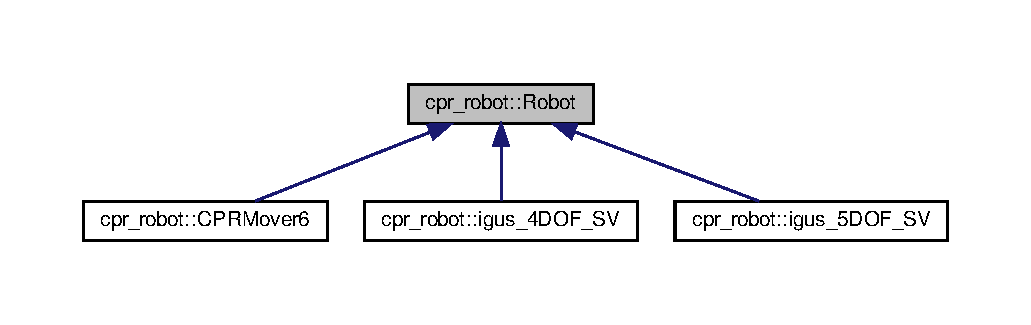
\includegraphics[width=350pt]{classcpr__robot_1_1Robot__inherit__graph}
\end{center}
\end{figure}
\subsection*{Public Member Functions}
\begin{DoxyCompactItemize}
\item 
void \textbf{ Init} ()
\begin{DoxyCompactList}\small\item\em Initializes the robot. Should be called after all robot parameters (gear ratios, ticks per motor rotation) have been set. Will call the virtual On\+Init method. \end{DoxyCompactList}\item 
void \textbf{ Publish\+State} ()
\begin{DoxyCompactList}\small\item\em Publishes the current state of the robot on the /joint\+\_\+states and /\+Robot\+State R\+OS topics. \end{DoxyCompactList}\item 
void \textbf{ Read} ()
\begin{DoxyCompactList}\small\item\em Reads the current state of the robot from the firmware. \end{DoxyCompactList}\item 
void \textbf{ Write} ()
\begin{DoxyCompactList}\small\item\em Sends the current motion commands to the firmware in the modules that are controlling the motors of the robot. \end{DoxyCompactList}\item 
virtual \textbf{ $\sim$\+Robot} ()
\begin{DoxyCompactList}\small\item\em Destructor of the \doxyref{Robot}{p.}{classcpr__robot_1_1Robot} class. \end{DoxyCompactList}\end{DoxyCompactItemize}
\subsection*{Static Public Attributes}
\begin{DoxyCompactItemize}
\item 
static constexpr uint32\+\_\+t \textbf{ C\+O\+M\+M\+A\+N\+D\+\_\+\+C\+O\+N\+N\+E\+CT} =1
\begin{DoxyCompactList}\small\item\em Command requesting that connection should be established with all modules controlling the robot. \end{DoxyCompactList}\item 
static constexpr uint32\+\_\+t \textbf{ C\+O\+M\+M\+A\+N\+D\+\_\+\+D\+I\+S\+A\+B\+LE} =4
\begin{DoxyCompactList}\small\item\em Command requesting that motor motion should be disabled for all joints. \end{DoxyCompactList}\item 
static constexpr uint32\+\_\+t \textbf{ C\+O\+M\+M\+A\+N\+D\+\_\+\+D\+I\+S\+C\+O\+N\+N\+E\+CT} =2
\begin{DoxyCompactList}\small\item\em Command requesting that the connections to all modules controlling the robot should be closed. \end{DoxyCompactList}\item 
static constexpr uint32\+\_\+t \textbf{ C\+O\+M\+M\+A\+N\+D\+\_\+\+E\+N\+A\+B\+LE} =3
\begin{DoxyCompactList}\small\item\em Command requesting that motor motion should be enabled for all joints. \end{DoxyCompactList}\item 
static constexpr uint32\+\_\+t \textbf{ C\+O\+M\+M\+A\+N\+D\+\_\+\+O\+V\+E\+R\+R\+I\+DE} =5
\begin{DoxyCompactList}\small\item\em Command sending a new override value contolling the speed of the joints. \end{DoxyCompactList}\item 
static constexpr uint32\+\_\+t \textbf{ C\+O\+M\+M\+A\+N\+D\+\_\+\+S\+E\+T\+Z\+E\+RO} =7
\begin{DoxyCompactList}\small\item\em Command requesting that the encoder positions of all joints should be reset. \end{DoxyCompactList}\item 
static constexpr uint32\+\_\+t \textbf{ C\+O\+M\+M\+A\+N\+D\+\_\+\+S\+T\+A\+R\+T\+R\+E\+F\+E\+R\+E\+N\+C\+I\+NG} =6
\begin{DoxyCompactList}\small\item\em Command requesting the referencing procedure to be initiated for all joints. \end{DoxyCompactList}\item 
static constexpr uint32\+\_\+t \textbf{ S\+T\+A\+T\+U\+S\+F\+L\+A\+G\+\_\+\+D\+I\+S\+C\+O\+N\+N\+E\+C\+T\+ED} =0x00000100
\begin{DoxyCompactList}\small\item\em Statusflag indicating that at least one of the modules that is controlling the robot is not connected. \end{DoxyCompactList}\end{DoxyCompactItemize}
\subsection*{Protected Member Functions}
\begin{DoxyCompactItemize}
\item 
double \textbf{ get\+\_\+\+Gear\+Ratio} (const size\+\_\+t joint\+Id)
\begin{DoxyCompactList}\small\item\em Gets the gear ratio of a specific joint. \end{DoxyCompactList}\item 
const std\+::string \& \textbf{ get\+\_\+\+Joint\+Name} (const size\+\_\+t joint\+Id)
\begin{DoxyCompactList}\small\item\em Gets the name of a specific joint that is used for communication over R\+OS topics and services. \end{DoxyCompactList}\item 
double \textbf{ get\+\_\+\+Max\+Position} (const size\+\_\+t joint\+Id) const
\begin{DoxyCompactList}\small\item\em Gets the upper bound for the position of a specific joint. \end{DoxyCompactList}\item 
double \textbf{ get\+\_\+\+Max\+Velocity} (const size\+\_\+t joint\+Id)
\begin{DoxyCompactList}\small\item\em Gets the maximal allowed angular velocity of a specific joint. \end{DoxyCompactList}\item 
double \textbf{ get\+\_\+\+Min\+Position} (const size\+\_\+t joint\+Id) const
\begin{DoxyCompactList}\small\item\em Gets the lower bound for the position of a specific joint. \end{DoxyCompactList}\item 
const std\+::string \& \textbf{ get\+\_\+\+Model\+Name} ()
\begin{DoxyCompactList}\small\item\em Gets the model designatin of the robot. \end{DoxyCompactList}\item 
int32\+\_\+t \textbf{ get\+\_\+\+Motor\+Offset} (const size\+\_\+t joint\+Id)
\begin{DoxyCompactList}\small\item\em Gets the zero position of the motor of a specific joint. \end{DoxyCompactList}\item 
double \textbf{ get\+\_\+\+Override} () const
\begin{DoxyCompactList}\small\item\em Gets the override value used to control the speed of the joints. \end{DoxyCompactList}\item 
int32\+\_\+t \textbf{ get\+\_\+\+Ticks\+Per\+Motor\+Rotation} (const size\+\_\+t joint\+Id)
\begin{DoxyCompactList}\small\item\em Gets the number of encoder ticks representic one rotation of the motor for a specific joint. \end{DoxyCompactList}\item 
virtual void \textbf{ On\+Init} ()
\begin{DoxyCompactList}\small\item\em Initializes the robot. \end{DoxyCompactList}\item 
\textbf{ Robot} (size\+\_\+t count\+Joints)
\item 
void \textbf{ set\+\_\+\+Gear\+Ratio} (const size\+\_\+t joint\+Id, const double ratio)
\begin{DoxyCompactList}\small\item\em Sets the gear ratio of a specific joint. \end{DoxyCompactList}\item 
void \textbf{ set\+\_\+\+Joint\+Name} (const size\+\_\+t joint\+Id, const std\+::string \&name)
\begin{DoxyCompactList}\small\item\em Sets the name of a specific joint that will be used for communication over R\+OS topics and services. \end{DoxyCompactList}\item 
void \textbf{ set\+\_\+\+Max\+Position} (const size\+\_\+t joint\+Id, const double position)
\begin{DoxyCompactList}\small\item\em Sets the upper bound for the position of a specific joint. \end{DoxyCompactList}\item 
void \textbf{ set\+\_\+\+Max\+Velocity} (const size\+\_\+t joint\+Id, const double velocity)
\begin{DoxyCompactList}\small\item\em Sets the maximal allowed angular velocity of a specific joint. \end{DoxyCompactList}\item 
void \textbf{ set\+\_\+\+Min\+Position} (const size\+\_\+t joint\+Id, const double position)
\begin{DoxyCompactList}\small\item\em Sets the lower bound for the position of a specific joint. \end{DoxyCompactList}\item 
void \textbf{ set\+\_\+\+Model\+Name} (const std\+::string \&name)
\begin{DoxyCompactList}\small\item\em Sets the model designatin of the robot. Should be called before the Init method is called. \end{DoxyCompactList}\item 
void \textbf{ set\+\_\+\+Motor\+Offset} (const size\+\_\+t joint\+Id, const int32\+\_\+t ticks)
\begin{DoxyCompactList}\small\item\em Sets the zero position of the motor of a specific joint. \end{DoxyCompactList}\item 
void \textbf{ set\+\_\+\+Override} (const double override)
\begin{DoxyCompactList}\small\item\em Sets the override value used to control the speed of the joints. \end{DoxyCompactList}\item 
void \textbf{ set\+\_\+\+Ticks\+Per\+Motor\+Rotation} (const size\+\_\+t joint\+Id, const int32\+\_\+t ticks)
\begin{DoxyCompactList}\small\item\em Sets the number of encoder ticks representic one rotation of the motor for a specific joint. \end{DoxyCompactList}\end{DoxyCompactItemize}
\subsection*{Private Member Functions}
\begin{DoxyCompactItemize}
\item 
bool \textbf{ Get\+Joint\+Info\+Handler} (cpr\+\_\+robot\+::\+Get\+Joint\+Info\+::\+Request \&req, cpr\+\_\+robot\+::\+Get\+Joint\+Info\+::\+Response \&res)
\begin{DoxyCompactList}\small\item\em Callback function handling requests to the /\+Get\+Joint\+Info R\+OS service. \end{DoxyCompactList}\item 
bool \textbf{ Get\+Robot\+Info\+Handler} (cpr\+\_\+robot\+::\+Get\+Robot\+Info\+::\+Request \&req, cpr\+\_\+robot\+::\+Get\+Robot\+Info\+::\+Response \&res)
\begin{DoxyCompactList}\small\item\em Callback function handling requests to the /\+Get\+Robot\+Info R\+OS service. \end{DoxyCompactList}\item 
bool \textbf{ Robot\+Command\+Handler} (cpr\+\_\+robot\+::\+Robot\+Command\+::\+Request \&req, cpr\+\_\+robot\+::\+Robot\+Command\+::\+Response \&res)
\begin{DoxyCompactList}\small\item\em Callback function handling requests to the /\+Robot\+Command R\+OS service. \end{DoxyCompactList}\end{DoxyCompactItemize}
\subsection*{Private Attributes}
\begin{DoxyCompactItemize}
\item 
\textbf{ Bus} \textbf{ m\+\_\+\+Bus}
\begin{DoxyCompactList}\small\item\em Instance of the \doxyref{Bus}{p.}{classcpr__robot_1_1Bus} class that will be used to communicate with the firmware of the modules that are controlling the robot. \end{DoxyCompactList}\item 
const size\+\_\+t \textbf{ m\+\_\+\+Count\+Joints}
\begin{DoxyCompactList}\small\item\em The number of joints of the robot. \end{DoxyCompactList}\item 
ros\+::\+Service\+Server \textbf{ m\+\_\+\+Get\+Joint\+Info\+Server}
\begin{DoxyCompactList}\small\item\em Provides information about a a specific joint (name, type) over the /\+Get\+Joint\+Info R\+OS service. \end{DoxyCompactList}\item 
ros\+::\+Service\+Server \textbf{ m\+\_\+\+Get\+Robot\+Info\+Server}
\begin{DoxyCompactList}\small\item\em Provides information about the robot (number of joints, model deisgnation) over the /\+Get\+Robot\+Info R\+OS service. \end{DoxyCompactList}\item 
ros\+::\+Publisher \textbf{ m\+\_\+\+Joint\+State\+Publisher}
\begin{DoxyCompactList}\small\item\em Publisher that will publish the state of all joints on the /joint\+\_\+states R\+OS topic. \end{DoxyCompactList}\item 
std\+::string \textbf{ m\+\_\+\+Model\+Name}
\begin{DoxyCompactList}\small\item\em The model designation of the robot. \end{DoxyCompactList}\item 
ros\+::\+Node\+Handle \textbf{ m\+\_\+\+Node}
\begin{DoxyCompactList}\small\item\em A handle to the current R\+OS node. \end{DoxyCompactList}\item 
double \textbf{ m\+\_\+\+Override}
\begin{DoxyCompactList}\small\item\em The current override value used to control the speed of the joints. \end{DoxyCompactList}\item 
\textbf{ Joint} $\ast$$\ast$ \textbf{ m\+\_\+p\+Joints}
\begin{DoxyCompactList}\small\item\em Pointer to an array of instances of the \doxyref{Joint}{p.}{classcpr__robot_1_1Joint} class. One entry per joint. \end{DoxyCompactList}\item 
ros\+::\+Service\+Server \textbf{ m\+\_\+\+Robot\+Command\+Server}
\begin{DoxyCompactList}\small\item\em Allows the robot to receive commands over the /\+Robot\+Command R\+OS service. \end{DoxyCompactList}\item 
ros\+::\+Publisher \textbf{ m\+\_\+\+Robot\+State\+Publisher}
\begin{DoxyCompactList}\small\item\em Publisher that will publish the state of the robot (error flags, etc.) on the /\+Robot\+State R\+OS topic. \end{DoxyCompactList}\end{DoxyCompactItemize}


\subsection{Detailed Description}
Abstract class representing a generic robot. 

This class hold all information associated with a robot\+: joints, connection status and information about the specific model. It serves as base class for model specific implementations and handles publishing information on R\+OS topics and services as well as listening to R\+OS topics for commands. 

Definition at line 9 of file Robot.\+h.



\subsection{Constructor \& Destructor Documentation}
\mbox{\label{classcpr__robot_1_1Robot_ab55f75f535333cebfd66666e098f49af}} 
\index{cpr\+\_\+robot\+::\+Robot@{cpr\+\_\+robot\+::\+Robot}!Robot@{Robot}}
\index{Robot@{Robot}!cpr\+\_\+robot\+::\+Robot@{cpr\+\_\+robot\+::\+Robot}}
\subsubsection{Robot()}
{\footnotesize\ttfamily cpr\+\_\+robot\+::\+Robot\+::\+Robot (\begin{DoxyParamCaption}\item[{size\+\_\+t}]{count\+Joints }\end{DoxyParamCaption})\hspace{0.3cm}{\ttfamily [protected]}}



Definition at line 53 of file Robot.\+cpp.

\mbox{\label{classcpr__robot_1_1Robot_af4a65cf0b26df1fd2fe990ab62f1791e}} 
\index{cpr\+\_\+robot\+::\+Robot@{cpr\+\_\+robot\+::\+Robot}!````~Robot@{$\sim$\+Robot}}
\index{````~Robot@{$\sim$\+Robot}!cpr\+\_\+robot\+::\+Robot@{cpr\+\_\+robot\+::\+Robot}}
\subsubsection{$\sim$\+Robot()}
{\footnotesize\ttfamily cpr\+\_\+robot\+::\+Robot\+::$\sim$\+Robot (\begin{DoxyParamCaption}{ }\end{DoxyParamCaption})\hspace{0.3cm}{\ttfamily [virtual]}}



Destructor of the \doxyref{Robot}{p.}{classcpr__robot_1_1Robot} class. 



Definition at line 120 of file Robot.\+cpp.



\subsection{Member Function Documentation}
\mbox{\label{classcpr__robot_1_1Robot_a50843a2467d9eb0b8a709b6512b3bdc9}} 
\index{cpr\+\_\+robot\+::\+Robot@{cpr\+\_\+robot\+::\+Robot}!get\+\_\+\+Gear\+Ratio@{get\+\_\+\+Gear\+Ratio}}
\index{get\+\_\+\+Gear\+Ratio@{get\+\_\+\+Gear\+Ratio}!cpr\+\_\+robot\+::\+Robot@{cpr\+\_\+robot\+::\+Robot}}
\subsubsection{get\+\_\+\+Gear\+Ratio()}
{\footnotesize\ttfamily double cpr\+\_\+robot\+::\+Robot\+::get\+\_\+\+Gear\+Ratio (\begin{DoxyParamCaption}\item[{const size\+\_\+t}]{joint\+Id }\end{DoxyParamCaption})\hspace{0.3cm}{\ttfamily [protected]}}



Gets the gear ratio of a specific joint. 


\begin{DoxyParams}{Parameters}
{\em joint\+Id} & The ID of the joint for which the gear ratio is to be retrieved. \\
\hline
\end{DoxyParams}
\begin{DoxyReturn}{Returns}
The gear ratio of the joint. 
\end{DoxyReturn}


Definition at line 279 of file Robot.\+cpp.

\mbox{\label{classcpr__robot_1_1Robot_a239f53f82185d265d555705c032bdedf}} 
\index{cpr\+\_\+robot\+::\+Robot@{cpr\+\_\+robot\+::\+Robot}!get\+\_\+\+Joint\+Name@{get\+\_\+\+Joint\+Name}}
\index{get\+\_\+\+Joint\+Name@{get\+\_\+\+Joint\+Name}!cpr\+\_\+robot\+::\+Robot@{cpr\+\_\+robot\+::\+Robot}}
\subsubsection{get\+\_\+\+Joint\+Name()}
{\footnotesize\ttfamily const std\+::string \& cpr\+\_\+robot\+::\+Robot\+::get\+\_\+\+Joint\+Name (\begin{DoxyParamCaption}\item[{const size\+\_\+t}]{joint\+Id }\end{DoxyParamCaption})\hspace{0.3cm}{\ttfamily [protected]}}



Gets the name of a specific joint that is used for communication over R\+OS topics and services. 


\begin{DoxyParams}{Parameters}
{\em joint\+Id} & The ID of the joint whos name is to be retrieved. \\
\hline
\end{DoxyParams}
\begin{DoxyReturn}{Returns}
The name of the joint. 
\end{DoxyReturn}


Definition at line 261 of file Robot.\+cpp.

\mbox{\label{classcpr__robot_1_1Robot_a3c17c74b7b0e496140ae63ff5ee9215e}} 
\index{cpr\+\_\+robot\+::\+Robot@{cpr\+\_\+robot\+::\+Robot}!get\+\_\+\+Max\+Position@{get\+\_\+\+Max\+Position}}
\index{get\+\_\+\+Max\+Position@{get\+\_\+\+Max\+Position}!cpr\+\_\+robot\+::\+Robot@{cpr\+\_\+robot\+::\+Robot}}
\subsubsection{get\+\_\+\+Max\+Position()}
{\footnotesize\ttfamily double cpr\+\_\+robot\+::\+Robot\+::get\+\_\+\+Max\+Position (\begin{DoxyParamCaption}\item[{const size\+\_\+t}]{joint\+Id }\end{DoxyParamCaption}) const\hspace{0.3cm}{\ttfamily [protected]}}



Gets the upper bound for the position of a specific joint. 


\begin{DoxyParams}{Parameters}
{\em joint\+Id} & The ID of the joint for wich the upper bound is to be retrieved. \\
\hline
\end{DoxyParams}
\begin{DoxyReturn}{Returns}
The current maximum allowed position of the joint. Measured in degrees. 
\end{DoxyReturn}


Definition at line 167 of file Robot.\+cpp.

\mbox{\label{classcpr__robot_1_1Robot_a9bdc22a8556d2c8bef49d95883f9e89b}} 
\index{cpr\+\_\+robot\+::\+Robot@{cpr\+\_\+robot\+::\+Robot}!get\+\_\+\+Max\+Velocity@{get\+\_\+\+Max\+Velocity}}
\index{get\+\_\+\+Max\+Velocity@{get\+\_\+\+Max\+Velocity}!cpr\+\_\+robot\+::\+Robot@{cpr\+\_\+robot\+::\+Robot}}
\subsubsection{get\+\_\+\+Max\+Velocity()}
{\footnotesize\ttfamily double cpr\+\_\+robot\+::\+Robot\+::get\+\_\+\+Max\+Velocity (\begin{DoxyParamCaption}\item[{const size\+\_\+t}]{joint\+Id }\end{DoxyParamCaption})\hspace{0.3cm}{\ttfamily [protected]}}



Gets the maximal allowed angular velocity of a specific joint. 


\begin{DoxyParams}{Parameters}
{\em joint\+Id} & The ID of the joint for which the maximal angular velocity is to be retrieved. \\
\hline
\end{DoxyParams}
\begin{DoxyReturn}{Returns}
The maximal angular velocity measured in degrees per second. 
\end{DoxyReturn}


Definition at line 315 of file Robot.\+cpp.

\mbox{\label{classcpr__robot_1_1Robot_a927a6455715d29289e3c587022be498e}} 
\index{cpr\+\_\+robot\+::\+Robot@{cpr\+\_\+robot\+::\+Robot}!get\+\_\+\+Min\+Position@{get\+\_\+\+Min\+Position}}
\index{get\+\_\+\+Min\+Position@{get\+\_\+\+Min\+Position}!cpr\+\_\+robot\+::\+Robot@{cpr\+\_\+robot\+::\+Robot}}
\subsubsection{get\+\_\+\+Min\+Position()}
{\footnotesize\ttfamily double cpr\+\_\+robot\+::\+Robot\+::get\+\_\+\+Min\+Position (\begin{DoxyParamCaption}\item[{const size\+\_\+t}]{joint\+Id }\end{DoxyParamCaption}) const\hspace{0.3cm}{\ttfamily [protected]}}



Gets the lower bound for the position of a specific joint. 


\begin{DoxyParams}{Parameters}
{\em joint\+Id} & The ID of the joint for wich the lower bound is to be retrieved. \\
\hline
\end{DoxyParams}
\begin{DoxyReturn}{Returns}
The current minimum allowed position of the joint. Measured in degrees. 
\end{DoxyReturn}


Definition at line 185 of file Robot.\+cpp.

\mbox{\label{classcpr__robot_1_1Robot_a78701a85bb62aa3656ec34844a98a0c4}} 
\index{cpr\+\_\+robot\+::\+Robot@{cpr\+\_\+robot\+::\+Robot}!get\+\_\+\+Model\+Name@{get\+\_\+\+Model\+Name}}
\index{get\+\_\+\+Model\+Name@{get\+\_\+\+Model\+Name}!cpr\+\_\+robot\+::\+Robot@{cpr\+\_\+robot\+::\+Robot}}
\subsubsection{get\+\_\+\+Model\+Name()}
{\footnotesize\ttfamily const std\+::string \& cpr\+\_\+robot\+::\+Robot\+::get\+\_\+\+Model\+Name (\begin{DoxyParamCaption}{ }\end{DoxyParamCaption})\hspace{0.3cm}{\ttfamily [protected]}}



Gets the model designatin of the robot. 

\begin{DoxyReturn}{Returns}
The model designation of the robot. 
\end{DoxyReturn}


Definition at line 46 of file Robot.\+cpp.

\mbox{\label{classcpr__robot_1_1Robot_a192a4a42112b292adf0ba693fbc78ded}} 
\index{cpr\+\_\+robot\+::\+Robot@{cpr\+\_\+robot\+::\+Robot}!get\+\_\+\+Motor\+Offset@{get\+\_\+\+Motor\+Offset}}
\index{get\+\_\+\+Motor\+Offset@{get\+\_\+\+Motor\+Offset}!cpr\+\_\+robot\+::\+Robot@{cpr\+\_\+robot\+::\+Robot}}
\subsubsection{get\+\_\+\+Motor\+Offset()}
{\footnotesize\ttfamily int32\+\_\+t cpr\+\_\+robot\+::\+Robot\+::get\+\_\+\+Motor\+Offset (\begin{DoxyParamCaption}\item[{const size\+\_\+t}]{joint\+Id }\end{DoxyParamCaption})\hspace{0.3cm}{\ttfamily [protected]}}



Gets the zero position of the motor of a specific joint. 


\begin{DoxyParams}{Parameters}
{\em joint\+Id} & The ID of the joint for which the zero position is to be retrieved. \\
\hline
\end{DoxyParams}
\begin{DoxyReturn}{Returns}
The current zero offset of the motor measured in encoder ticks. 
\end{DoxyReturn}


Definition at line 213 of file Robot.\+cpp.

\mbox{\label{classcpr__robot_1_1Robot_a9497c983bd4c42b35b2627396e8976e5}} 
\index{cpr\+\_\+robot\+::\+Robot@{cpr\+\_\+robot\+::\+Robot}!get\+\_\+\+Override@{get\+\_\+\+Override}}
\index{get\+\_\+\+Override@{get\+\_\+\+Override}!cpr\+\_\+robot\+::\+Robot@{cpr\+\_\+robot\+::\+Robot}}
\subsubsection{get\+\_\+\+Override()}
{\footnotesize\ttfamily double cpr\+\_\+robot\+::\+Robot\+::get\+\_\+\+Override (\begin{DoxyParamCaption}{ }\end{DoxyParamCaption}) const\hspace{0.3cm}{\ttfamily [protected]}}



Gets the override value used to control the speed of the joints. 

\begin{DoxyReturn}{Returns}
The current override value. 
\end{DoxyReturn}


Definition at line 136 of file Robot.\+cpp.

\mbox{\label{classcpr__robot_1_1Robot_a4e52f9c1a6be296538626649f356fa12}} 
\index{cpr\+\_\+robot\+::\+Robot@{cpr\+\_\+robot\+::\+Robot}!get\+\_\+\+Ticks\+Per\+Motor\+Rotation@{get\+\_\+\+Ticks\+Per\+Motor\+Rotation}}
\index{get\+\_\+\+Ticks\+Per\+Motor\+Rotation@{get\+\_\+\+Ticks\+Per\+Motor\+Rotation}!cpr\+\_\+robot\+::\+Robot@{cpr\+\_\+robot\+::\+Robot}}
\subsubsection{get\+\_\+\+Ticks\+Per\+Motor\+Rotation()}
{\footnotesize\ttfamily int32\+\_\+t cpr\+\_\+robot\+::\+Robot\+::get\+\_\+\+Ticks\+Per\+Motor\+Rotation (\begin{DoxyParamCaption}\item[{const size\+\_\+t}]{joint\+Id }\end{DoxyParamCaption})\hspace{0.3cm}{\ttfamily [protected]}}



Gets the number of encoder ticks representic one rotation of the motor for a specific joint. 


\begin{DoxyParams}{Parameters}
{\em joint\+Id} & The ID of the joint for which the ticks per rotation is to be retrieved. \\
\hline
\end{DoxyParams}
\begin{DoxyReturn}{Returns}
The number of encoder ticks representing exactly one rotation of the motor. 
\end{DoxyReturn}


Definition at line 297 of file Robot.\+cpp.

\mbox{\label{classcpr__robot_1_1Robot_ae1b76ade14340df725b17c7da4e489fb}} 
\index{cpr\+\_\+robot\+::\+Robot@{cpr\+\_\+robot\+::\+Robot}!Get\+Joint\+Info\+Handler@{Get\+Joint\+Info\+Handler}}
\index{Get\+Joint\+Info\+Handler@{Get\+Joint\+Info\+Handler}!cpr\+\_\+robot\+::\+Robot@{cpr\+\_\+robot\+::\+Robot}}
\subsubsection{Get\+Joint\+Info\+Handler()}
{\footnotesize\ttfamily bool cpr\+\_\+robot\+::\+Robot\+::\+Get\+Joint\+Info\+Handler (\begin{DoxyParamCaption}\item[{cpr\+\_\+robot\+::\+Get\+Joint\+Info\+::\+Request \&}]{req,  }\item[{cpr\+\_\+robot\+::\+Get\+Joint\+Info\+::\+Response \&}]{res }\end{DoxyParamCaption})\hspace{0.3cm}{\ttfamily [private]}}



Callback function handling requests to the /\+Get\+Joint\+Info R\+OS service. 


\begin{DoxyParams}{Parameters}
{\em req} & The request to be handled. \\
\hline
{\em res} & The answer that will be returned to the request. \\
\hline
\end{DoxyParams}
\begin{DoxyReturn}{Returns}
Returns true if the request has been handled successfully, elsewise returns false. 
\end{DoxyReturn}


Definition at line 22 of file Robot.\+cpp.

\mbox{\label{classcpr__robot_1_1Robot_add37ad3b30ae5a56dc9a937f14046b82}} 
\index{cpr\+\_\+robot\+::\+Robot@{cpr\+\_\+robot\+::\+Robot}!Get\+Robot\+Info\+Handler@{Get\+Robot\+Info\+Handler}}
\index{Get\+Robot\+Info\+Handler@{Get\+Robot\+Info\+Handler}!cpr\+\_\+robot\+::\+Robot@{cpr\+\_\+robot\+::\+Robot}}
\subsubsection{Get\+Robot\+Info\+Handler()}
{\footnotesize\ttfamily bool cpr\+\_\+robot\+::\+Robot\+::\+Get\+Robot\+Info\+Handler (\begin{DoxyParamCaption}\item[{cpr\+\_\+robot\+::\+Get\+Robot\+Info\+::\+Request \&}]{req,  }\item[{cpr\+\_\+robot\+::\+Get\+Robot\+Info\+::\+Response \&}]{res }\end{DoxyParamCaption})\hspace{0.3cm}{\ttfamily [private]}}



Callback function handling requests to the /\+Get\+Robot\+Info R\+OS service. 


\begin{DoxyParams}{Parameters}
{\em req} & The request to be handled. \\
\hline
{\em res} & The answer that will be returned to the request. \\
\hline
\end{DoxyParams}
\begin{DoxyReturn}{Returns}
Returns true if the request has been handled successfully, elsewise returns false. 
\end{DoxyReturn}


Definition at line 11 of file Robot.\+cpp.

\mbox{\label{classcpr__robot_1_1Robot_a469ed567a445caf868e8154997c8ba76}} 
\index{cpr\+\_\+robot\+::\+Robot@{cpr\+\_\+robot\+::\+Robot}!Init@{Init}}
\index{Init@{Init}!cpr\+\_\+robot\+::\+Robot@{cpr\+\_\+robot\+::\+Robot}}
\subsubsection{Init()}
{\footnotesize\ttfamily void cpr\+\_\+robot\+::\+Robot\+::\+Init (\begin{DoxyParamCaption}{ }\end{DoxyParamCaption})}



Initializes the robot. Should be called after all robot parameters (gear ratios, ticks per motor rotation) have been set. Will call the virtual On\+Init method. 



Definition at line 235 of file Robot.\+cpp.

\mbox{\label{classcpr__robot_1_1Robot_a93a9ecdc4161e969f31d37e073c9ea7b}} 
\index{cpr\+\_\+robot\+::\+Robot@{cpr\+\_\+robot\+::\+Robot}!On\+Init@{On\+Init}}
\index{On\+Init@{On\+Init}!cpr\+\_\+robot\+::\+Robot@{cpr\+\_\+robot\+::\+Robot}}
\subsubsection{On\+Init()}
{\footnotesize\ttfamily void cpr\+\_\+robot\+::\+Robot\+::\+On\+Init (\begin{DoxyParamCaption}{ }\end{DoxyParamCaption})\hspace{0.3cm}{\ttfamily [protected]}, {\ttfamily [virtual]}}



Initializes the robot. 

Should be called after all robot parameters (gear ratios, ticks per motor rotation) have been set. 

Definition at line 243 of file Robot.\+cpp.

\mbox{\label{classcpr__robot_1_1Robot_a105157bf29fc8567601655805cd29906}} 
\index{cpr\+\_\+robot\+::\+Robot@{cpr\+\_\+robot\+::\+Robot}!Publish\+State@{Publish\+State}}
\index{Publish\+State@{Publish\+State}!cpr\+\_\+robot\+::\+Robot@{cpr\+\_\+robot\+::\+Robot}}
\subsubsection{Publish\+State()}
{\footnotesize\ttfamily void cpr\+\_\+robot\+::\+Robot\+::\+Publish\+State (\begin{DoxyParamCaption}{ }\end{DoxyParamCaption})}



Publishes the current state of the robot on the /joint\+\_\+states and /\+Robot\+State R\+OS topics. 



Definition at line 142 of file Robot.\+cpp.

\mbox{\label{classcpr__robot_1_1Robot_a7daf552f78f48b9c155d4d6708c49e2b}} 
\index{cpr\+\_\+robot\+::\+Robot@{cpr\+\_\+robot\+::\+Robot}!Read@{Read}}
\index{Read@{Read}!cpr\+\_\+robot\+::\+Robot@{cpr\+\_\+robot\+::\+Robot}}
\subsubsection{Read()}
{\footnotesize\ttfamily void cpr\+\_\+robot\+::\+Robot\+::\+Read (\begin{DoxyParamCaption}{ }\end{DoxyParamCaption})}



Reads the current state of the robot from the firmware. 



Definition at line 220 of file Robot.\+cpp.

\mbox{\label{classcpr__robot_1_1Robot_ac8bc2d6eb9447d1c70673186cee17174}} 
\index{cpr\+\_\+robot\+::\+Robot@{cpr\+\_\+robot\+::\+Robot}!Robot\+Command\+Handler@{Robot\+Command\+Handler}}
\index{Robot\+Command\+Handler@{Robot\+Command\+Handler}!cpr\+\_\+robot\+::\+Robot@{cpr\+\_\+robot\+::\+Robot}}
\subsubsection{Robot\+Command\+Handler()}
{\footnotesize\ttfamily bool cpr\+\_\+robot\+::\+Robot\+::\+Robot\+Command\+Handler (\begin{DoxyParamCaption}\item[{cpr\+\_\+robot\+::\+Robot\+Command\+::\+Request \&}]{req,  }\item[{cpr\+\_\+robot\+::\+Robot\+Command\+::\+Response \&}]{res }\end{DoxyParamCaption})\hspace{0.3cm}{\ttfamily [private]}}



Callback function handling requests to the /\+Robot\+Command R\+OS service. 


\begin{DoxyParams}{Parameters}
{\em req} & The request to be handled. \\
\hline
{\em res} & The answer that will be returned to the request. \\
\hline
\end{DoxyParams}
\begin{DoxyReturn}{Returns}
Returns true if the request has been handled successfully, elsewise returns false. 
\end{DoxyReturn}


Definition at line 73 of file Robot.\+cpp.

\mbox{\label{classcpr__robot_1_1Robot_a8a2aa193af46dae4a45308bbf59ffad7}} 
\index{cpr\+\_\+robot\+::\+Robot@{cpr\+\_\+robot\+::\+Robot}!set\+\_\+\+Gear\+Ratio@{set\+\_\+\+Gear\+Ratio}}
\index{set\+\_\+\+Gear\+Ratio@{set\+\_\+\+Gear\+Ratio}!cpr\+\_\+robot\+::\+Robot@{cpr\+\_\+robot\+::\+Robot}}
\subsubsection{set\+\_\+\+Gear\+Ratio()}
{\footnotesize\ttfamily void cpr\+\_\+robot\+::\+Robot\+::set\+\_\+\+Gear\+Ratio (\begin{DoxyParamCaption}\item[{const size\+\_\+t}]{joint\+Id,  }\item[{const double}]{ratio }\end{DoxyParamCaption})\hspace{0.3cm}{\ttfamily [protected]}}



Sets the gear ratio of a specific joint. 


\begin{DoxyParams}{Parameters}
{\em joint\+Id} & The ID of the joint for which the gear ratio is to be set. \\
\hline
{\em ratio} & The gear ratio of for the joint. \\
\hline
\end{DoxyParams}


Definition at line 270 of file Robot.\+cpp.

\mbox{\label{classcpr__robot_1_1Robot_ad579a76d0f218169d98783e278855189}} 
\index{cpr\+\_\+robot\+::\+Robot@{cpr\+\_\+robot\+::\+Robot}!set\+\_\+\+Joint\+Name@{set\+\_\+\+Joint\+Name}}
\index{set\+\_\+\+Joint\+Name@{set\+\_\+\+Joint\+Name}!cpr\+\_\+robot\+::\+Robot@{cpr\+\_\+robot\+::\+Robot}}
\subsubsection{set\+\_\+\+Joint\+Name()}
{\footnotesize\ttfamily void cpr\+\_\+robot\+::\+Robot\+::set\+\_\+\+Joint\+Name (\begin{DoxyParamCaption}\item[{const size\+\_\+t}]{joint\+Id,  }\item[{const std\+::string \&}]{name }\end{DoxyParamCaption})\hspace{0.3cm}{\ttfamily [protected]}}



Sets the name of a specific joint that will be used for communication over R\+OS topics and services. 


\begin{DoxyParams}{Parameters}
{\em joint\+Id} & The ID of the joint for which the name should be set. \\
\hline
{\em name} & The desired name of the joint. \\
\hline
\end{DoxyParams}


Definition at line 252 of file Robot.\+cpp.

\mbox{\label{classcpr__robot_1_1Robot_abd8d0b83d5fac8210071ccfc72616b04}} 
\index{cpr\+\_\+robot\+::\+Robot@{cpr\+\_\+robot\+::\+Robot}!set\+\_\+\+Max\+Position@{set\+\_\+\+Max\+Position}}
\index{set\+\_\+\+Max\+Position@{set\+\_\+\+Max\+Position}!cpr\+\_\+robot\+::\+Robot@{cpr\+\_\+robot\+::\+Robot}}
\subsubsection{set\+\_\+\+Max\+Position()}
{\footnotesize\ttfamily void cpr\+\_\+robot\+::\+Robot\+::set\+\_\+\+Max\+Position (\begin{DoxyParamCaption}\item[{const size\+\_\+t}]{joint\+Id,  }\item[{const double}]{position }\end{DoxyParamCaption})\hspace{0.3cm}{\ttfamily [protected]}}



Sets the upper bound for the position of a specific joint. 


\begin{DoxyParams}{Parameters}
{\em joint\+Id} & The ID of the joint for which the upper bound is to be set. \\
\hline
{\em position} & The new maximum allowed position of the joint. Measured in degrees. \\
\hline
\end{DoxyParams}


Definition at line 176 of file Robot.\+cpp.

\mbox{\label{classcpr__robot_1_1Robot_adb35aa432d6938e92bd36ede3fc307d0}} 
\index{cpr\+\_\+robot\+::\+Robot@{cpr\+\_\+robot\+::\+Robot}!set\+\_\+\+Max\+Velocity@{set\+\_\+\+Max\+Velocity}}
\index{set\+\_\+\+Max\+Velocity@{set\+\_\+\+Max\+Velocity}!cpr\+\_\+robot\+::\+Robot@{cpr\+\_\+robot\+::\+Robot}}
\subsubsection{set\+\_\+\+Max\+Velocity()}
{\footnotesize\ttfamily void cpr\+\_\+robot\+::\+Robot\+::set\+\_\+\+Max\+Velocity (\begin{DoxyParamCaption}\item[{const size\+\_\+t}]{joint\+Id,  }\item[{const double}]{velocity }\end{DoxyParamCaption})\hspace{0.3cm}{\ttfamily [protected]}}



Sets the maximal allowed angular velocity of a specific joint. 


\begin{DoxyParams}{Parameters}
{\em joint\+Id} & The ID of the joint for which the maximal angular velocity is to be set. \\
\hline
{\em velocity} & The maximal angular velocity measured in degrees per second. \\
\hline
\end{DoxyParams}


Definition at line 306 of file Robot.\+cpp.

\mbox{\label{classcpr__robot_1_1Robot_a0762f75b8aa28f40621ff48272eedcc0}} 
\index{cpr\+\_\+robot\+::\+Robot@{cpr\+\_\+robot\+::\+Robot}!set\+\_\+\+Min\+Position@{set\+\_\+\+Min\+Position}}
\index{set\+\_\+\+Min\+Position@{set\+\_\+\+Min\+Position}!cpr\+\_\+robot\+::\+Robot@{cpr\+\_\+robot\+::\+Robot}}
\subsubsection{set\+\_\+\+Min\+Position()}
{\footnotesize\ttfamily void cpr\+\_\+robot\+::\+Robot\+::set\+\_\+\+Min\+Position (\begin{DoxyParamCaption}\item[{const size\+\_\+t}]{joint\+Id,  }\item[{const double}]{position }\end{DoxyParamCaption})\hspace{0.3cm}{\ttfamily [protected]}}



Sets the lower bound for the position of a specific joint. 


\begin{DoxyParams}{Parameters}
{\em joint\+Id} & The ID of the joint for which the lower bound is to be set. \\
\hline
{\em position} & The new minimum allowed position of the joint. Measured in degrees. \\
\hline
\end{DoxyParams}


Definition at line 195 of file Robot.\+cpp.

\mbox{\label{classcpr__robot_1_1Robot_a20f2e89a4dd34f763e84b0bd4d1e4519}} 
\index{cpr\+\_\+robot\+::\+Robot@{cpr\+\_\+robot\+::\+Robot}!set\+\_\+\+Model\+Name@{set\+\_\+\+Model\+Name}}
\index{set\+\_\+\+Model\+Name@{set\+\_\+\+Model\+Name}!cpr\+\_\+robot\+::\+Robot@{cpr\+\_\+robot\+::\+Robot}}
\subsubsection{set\+\_\+\+Model\+Name()}
{\footnotesize\ttfamily void cpr\+\_\+robot\+::\+Robot\+::set\+\_\+\+Model\+Name (\begin{DoxyParamCaption}\item[{const std\+::string \&}]{name }\end{DoxyParamCaption})\hspace{0.3cm}{\ttfamily [protected]}}



Sets the model designatin of the robot. Should be called before the Init method is called. 


\begin{DoxyParams}{Parameters}
{\em name} & The model designation of the robot. \\
\hline
\end{DoxyParams}


Definition at line 39 of file Robot.\+cpp.

\mbox{\label{classcpr__robot_1_1Robot_a779097d72d10c99a744c422cee93886e}} 
\index{cpr\+\_\+robot\+::\+Robot@{cpr\+\_\+robot\+::\+Robot}!set\+\_\+\+Motor\+Offset@{set\+\_\+\+Motor\+Offset}}
\index{set\+\_\+\+Motor\+Offset@{set\+\_\+\+Motor\+Offset}!cpr\+\_\+robot\+::\+Robot@{cpr\+\_\+robot\+::\+Robot}}
\subsubsection{set\+\_\+\+Motor\+Offset()}
{\footnotesize\ttfamily void cpr\+\_\+robot\+::\+Robot\+::set\+\_\+\+Motor\+Offset (\begin{DoxyParamCaption}\item[{const size\+\_\+t}]{joint\+Id,  }\item[{const int32\+\_\+t}]{ticks }\end{DoxyParamCaption})\hspace{0.3cm}{\ttfamily [protected]}}



Sets the zero position of the motor of a specific joint. 


\begin{DoxyParams}{Parameters}
{\em joint\+Id} & The ID of the joint for which the zero position is to be set. \\
\hline
{\em ticks} & The new zero offset of the motor measured in encoder ticks. \\
\hline
\end{DoxyParams}


Definition at line 204 of file Robot.\+cpp.

\mbox{\label{classcpr__robot_1_1Robot_a01c11848076687d2f583aecacf4645f5}} 
\index{cpr\+\_\+robot\+::\+Robot@{cpr\+\_\+robot\+::\+Robot}!set\+\_\+\+Override@{set\+\_\+\+Override}}
\index{set\+\_\+\+Override@{set\+\_\+\+Override}!cpr\+\_\+robot\+::\+Robot@{cpr\+\_\+robot\+::\+Robot}}
\subsubsection{set\+\_\+\+Override()}
{\footnotesize\ttfamily void cpr\+\_\+robot\+::\+Robot\+::set\+\_\+\+Override (\begin{DoxyParamCaption}\item[{const double}]{override }\end{DoxyParamCaption})\hspace{0.3cm}{\ttfamily [protected]}}



Sets the override value used to control the speed of the joints. 


\begin{DoxyParams}{Parameters}
{\em override} & The new override value. Must be between 0 and 1. \\
\hline
\end{DoxyParams}


Definition at line 129 of file Robot.\+cpp.

\mbox{\label{classcpr__robot_1_1Robot_a15768cdfd403bce94757a3c8cd1c8207}} 
\index{cpr\+\_\+robot\+::\+Robot@{cpr\+\_\+robot\+::\+Robot}!set\+\_\+\+Ticks\+Per\+Motor\+Rotation@{set\+\_\+\+Ticks\+Per\+Motor\+Rotation}}
\index{set\+\_\+\+Ticks\+Per\+Motor\+Rotation@{set\+\_\+\+Ticks\+Per\+Motor\+Rotation}!cpr\+\_\+robot\+::\+Robot@{cpr\+\_\+robot\+::\+Robot}}
\subsubsection{set\+\_\+\+Ticks\+Per\+Motor\+Rotation()}
{\footnotesize\ttfamily void cpr\+\_\+robot\+::\+Robot\+::set\+\_\+\+Ticks\+Per\+Motor\+Rotation (\begin{DoxyParamCaption}\item[{const size\+\_\+t}]{joint\+Id,  }\item[{const int32\+\_\+t}]{ticks }\end{DoxyParamCaption})\hspace{0.3cm}{\ttfamily [protected]}}



Sets the number of encoder ticks representic one rotation of the motor for a specific joint. 


\begin{DoxyParams}{Parameters}
{\em joint\+Id} & The ID of the joint for which the ticks per rotation is to be set. \\
\hline
{\em ticks} & The number of encoder ticks representing exactly one rotation of the motor. \\
\hline
\end{DoxyParams}


Definition at line 288 of file Robot.\+cpp.

\mbox{\label{classcpr__robot_1_1Robot_a813a91e6dfdd4d3d57618999eed008c6}} 
\index{cpr\+\_\+robot\+::\+Robot@{cpr\+\_\+robot\+::\+Robot}!Write@{Write}}
\index{Write@{Write}!cpr\+\_\+robot\+::\+Robot@{cpr\+\_\+robot\+::\+Robot}}
\subsubsection{Write()}
{\footnotesize\ttfamily void cpr\+\_\+robot\+::\+Robot\+::\+Write (\begin{DoxyParamCaption}{ }\end{DoxyParamCaption})}



Sends the current motion commands to the firmware in the modules that are controlling the motors of the robot. 



Definition at line 227 of file Robot.\+cpp.



\subsection{Member Data Documentation}
\mbox{\label{classcpr__robot_1_1Robot_aacbfb6bdcf0e25d80cb4b5cb9870bd73}} 
\index{cpr\+\_\+robot\+::\+Robot@{cpr\+\_\+robot\+::\+Robot}!C\+O\+M\+M\+A\+N\+D\+\_\+\+C\+O\+N\+N\+E\+CT@{C\+O\+M\+M\+A\+N\+D\+\_\+\+C\+O\+N\+N\+E\+CT}}
\index{C\+O\+M\+M\+A\+N\+D\+\_\+\+C\+O\+N\+N\+E\+CT@{C\+O\+M\+M\+A\+N\+D\+\_\+\+C\+O\+N\+N\+E\+CT}!cpr\+\_\+robot\+::\+Robot@{cpr\+\_\+robot\+::\+Robot}}
\subsubsection{C\+O\+M\+M\+A\+N\+D\+\_\+\+C\+O\+N\+N\+E\+CT}
{\footnotesize\ttfamily constexpr uint32\+\_\+t cpr\+\_\+robot\+::\+Robot\+::\+C\+O\+M\+M\+A\+N\+D\+\_\+\+C\+O\+N\+N\+E\+CT =1\hspace{0.3cm}{\ttfamily [static]}}



Command requesting that connection should be established with all modules controlling the robot. 



Definition at line 15 of file Robot.\+h.

\mbox{\label{classcpr__robot_1_1Robot_ab3428458b2f497a3d6b3f740b03c5f7c}} 
\index{cpr\+\_\+robot\+::\+Robot@{cpr\+\_\+robot\+::\+Robot}!C\+O\+M\+M\+A\+N\+D\+\_\+\+D\+I\+S\+A\+B\+LE@{C\+O\+M\+M\+A\+N\+D\+\_\+\+D\+I\+S\+A\+B\+LE}}
\index{C\+O\+M\+M\+A\+N\+D\+\_\+\+D\+I\+S\+A\+B\+LE@{C\+O\+M\+M\+A\+N\+D\+\_\+\+D\+I\+S\+A\+B\+LE}!cpr\+\_\+robot\+::\+Robot@{cpr\+\_\+robot\+::\+Robot}}
\subsubsection{C\+O\+M\+M\+A\+N\+D\+\_\+\+D\+I\+S\+A\+B\+LE}
{\footnotesize\ttfamily constexpr uint32\+\_\+t cpr\+\_\+robot\+::\+Robot\+::\+C\+O\+M\+M\+A\+N\+D\+\_\+\+D\+I\+S\+A\+B\+LE =4\hspace{0.3cm}{\ttfamily [static]}}



Command requesting that motor motion should be disabled for all joints. 



Definition at line 21 of file Robot.\+h.

\mbox{\label{classcpr__robot_1_1Robot_a09d49b8b87dd19199a44d4dd85ec86c2}} 
\index{cpr\+\_\+robot\+::\+Robot@{cpr\+\_\+robot\+::\+Robot}!C\+O\+M\+M\+A\+N\+D\+\_\+\+D\+I\+S\+C\+O\+N\+N\+E\+CT@{C\+O\+M\+M\+A\+N\+D\+\_\+\+D\+I\+S\+C\+O\+N\+N\+E\+CT}}
\index{C\+O\+M\+M\+A\+N\+D\+\_\+\+D\+I\+S\+C\+O\+N\+N\+E\+CT@{C\+O\+M\+M\+A\+N\+D\+\_\+\+D\+I\+S\+C\+O\+N\+N\+E\+CT}!cpr\+\_\+robot\+::\+Robot@{cpr\+\_\+robot\+::\+Robot}}
\subsubsection{C\+O\+M\+M\+A\+N\+D\+\_\+\+D\+I\+S\+C\+O\+N\+N\+E\+CT}
{\footnotesize\ttfamily constexpr uint32\+\_\+t cpr\+\_\+robot\+::\+Robot\+::\+C\+O\+M\+M\+A\+N\+D\+\_\+\+D\+I\+S\+C\+O\+N\+N\+E\+CT =2\hspace{0.3cm}{\ttfamily [static]}}



Command requesting that the connections to all modules controlling the robot should be closed. 



Definition at line 17 of file Robot.\+h.

\mbox{\label{classcpr__robot_1_1Robot_add9fc31ea8bd1978ef4b44cda5889304}} 
\index{cpr\+\_\+robot\+::\+Robot@{cpr\+\_\+robot\+::\+Robot}!C\+O\+M\+M\+A\+N\+D\+\_\+\+E\+N\+A\+B\+LE@{C\+O\+M\+M\+A\+N\+D\+\_\+\+E\+N\+A\+B\+LE}}
\index{C\+O\+M\+M\+A\+N\+D\+\_\+\+E\+N\+A\+B\+LE@{C\+O\+M\+M\+A\+N\+D\+\_\+\+E\+N\+A\+B\+LE}!cpr\+\_\+robot\+::\+Robot@{cpr\+\_\+robot\+::\+Robot}}
\subsubsection{C\+O\+M\+M\+A\+N\+D\+\_\+\+E\+N\+A\+B\+LE}
{\footnotesize\ttfamily constexpr uint32\+\_\+t cpr\+\_\+robot\+::\+Robot\+::\+C\+O\+M\+M\+A\+N\+D\+\_\+\+E\+N\+A\+B\+LE =3\hspace{0.3cm}{\ttfamily [static]}}



Command requesting that motor motion should be enabled for all joints. 



Definition at line 19 of file Robot.\+h.

\mbox{\label{classcpr__robot_1_1Robot_ae5f66b29ec11a0816c7622025dce51a8}} 
\index{cpr\+\_\+robot\+::\+Robot@{cpr\+\_\+robot\+::\+Robot}!C\+O\+M\+M\+A\+N\+D\+\_\+\+O\+V\+E\+R\+R\+I\+DE@{C\+O\+M\+M\+A\+N\+D\+\_\+\+O\+V\+E\+R\+R\+I\+DE}}
\index{C\+O\+M\+M\+A\+N\+D\+\_\+\+O\+V\+E\+R\+R\+I\+DE@{C\+O\+M\+M\+A\+N\+D\+\_\+\+O\+V\+E\+R\+R\+I\+DE}!cpr\+\_\+robot\+::\+Robot@{cpr\+\_\+robot\+::\+Robot}}
\subsubsection{C\+O\+M\+M\+A\+N\+D\+\_\+\+O\+V\+E\+R\+R\+I\+DE}
{\footnotesize\ttfamily constexpr uint32\+\_\+t cpr\+\_\+robot\+::\+Robot\+::\+C\+O\+M\+M\+A\+N\+D\+\_\+\+O\+V\+E\+R\+R\+I\+DE =5\hspace{0.3cm}{\ttfamily [static]}}



Command sending a new override value contolling the speed of the joints. 



Definition at line 23 of file Robot.\+h.

\mbox{\label{classcpr__robot_1_1Robot_a3199bceb08d000dc5acee602cf6e0dec}} 
\index{cpr\+\_\+robot\+::\+Robot@{cpr\+\_\+robot\+::\+Robot}!C\+O\+M\+M\+A\+N\+D\+\_\+\+S\+E\+T\+Z\+E\+RO@{C\+O\+M\+M\+A\+N\+D\+\_\+\+S\+E\+T\+Z\+E\+RO}}
\index{C\+O\+M\+M\+A\+N\+D\+\_\+\+S\+E\+T\+Z\+E\+RO@{C\+O\+M\+M\+A\+N\+D\+\_\+\+S\+E\+T\+Z\+E\+RO}!cpr\+\_\+robot\+::\+Robot@{cpr\+\_\+robot\+::\+Robot}}
\subsubsection{C\+O\+M\+M\+A\+N\+D\+\_\+\+S\+E\+T\+Z\+E\+RO}
{\footnotesize\ttfamily constexpr uint32\+\_\+t cpr\+\_\+robot\+::\+Robot\+::\+C\+O\+M\+M\+A\+N\+D\+\_\+\+S\+E\+T\+Z\+E\+RO =7\hspace{0.3cm}{\ttfamily [static]}}



Command requesting that the encoder positions of all joints should be reset. 



Definition at line 27 of file Robot.\+h.

\mbox{\label{classcpr__robot_1_1Robot_ad167012fbeb53ec7cea427acd51365c5}} 
\index{cpr\+\_\+robot\+::\+Robot@{cpr\+\_\+robot\+::\+Robot}!C\+O\+M\+M\+A\+N\+D\+\_\+\+S\+T\+A\+R\+T\+R\+E\+F\+E\+R\+E\+N\+C\+I\+NG@{C\+O\+M\+M\+A\+N\+D\+\_\+\+S\+T\+A\+R\+T\+R\+E\+F\+E\+R\+E\+N\+C\+I\+NG}}
\index{C\+O\+M\+M\+A\+N\+D\+\_\+\+S\+T\+A\+R\+T\+R\+E\+F\+E\+R\+E\+N\+C\+I\+NG@{C\+O\+M\+M\+A\+N\+D\+\_\+\+S\+T\+A\+R\+T\+R\+E\+F\+E\+R\+E\+N\+C\+I\+NG}!cpr\+\_\+robot\+::\+Robot@{cpr\+\_\+robot\+::\+Robot}}
\subsubsection{C\+O\+M\+M\+A\+N\+D\+\_\+\+S\+T\+A\+R\+T\+R\+E\+F\+E\+R\+E\+N\+C\+I\+NG}
{\footnotesize\ttfamily constexpr uint32\+\_\+t cpr\+\_\+robot\+::\+Robot\+::\+C\+O\+M\+M\+A\+N\+D\+\_\+\+S\+T\+A\+R\+T\+R\+E\+F\+E\+R\+E\+N\+C\+I\+NG =6\hspace{0.3cm}{\ttfamily [static]}}



Command requesting the referencing procedure to be initiated for all joints. 



Definition at line 25 of file Robot.\+h.

\mbox{\label{classcpr__robot_1_1Robot_afbeb2439782e91197f7584acc863a60d}} 
\index{cpr\+\_\+robot\+::\+Robot@{cpr\+\_\+robot\+::\+Robot}!m\+\_\+\+Bus@{m\+\_\+\+Bus}}
\index{m\+\_\+\+Bus@{m\+\_\+\+Bus}!cpr\+\_\+robot\+::\+Robot@{cpr\+\_\+robot\+::\+Robot}}
\subsubsection{m\+\_\+\+Bus}
{\footnotesize\ttfamily \textbf{ Bus} cpr\+\_\+robot\+::\+Robot\+::m\+\_\+\+Bus\hspace{0.3cm}{\ttfamily [private]}}



Instance of the \doxyref{Bus}{p.}{classcpr__robot_1_1Bus} class that will be used to communicate with the firmware of the modules that are controlling the robot. 



Definition at line 44 of file Robot.\+h.

\mbox{\label{classcpr__robot_1_1Robot_a2ffedf1435972a2c6976e8b7541ab257}} 
\index{cpr\+\_\+robot\+::\+Robot@{cpr\+\_\+robot\+::\+Robot}!m\+\_\+\+Count\+Joints@{m\+\_\+\+Count\+Joints}}
\index{m\+\_\+\+Count\+Joints@{m\+\_\+\+Count\+Joints}!cpr\+\_\+robot\+::\+Robot@{cpr\+\_\+robot\+::\+Robot}}
\subsubsection{m\+\_\+\+Count\+Joints}
{\footnotesize\ttfamily const size\+\_\+t cpr\+\_\+robot\+::\+Robot\+::m\+\_\+\+Count\+Joints\hspace{0.3cm}{\ttfamily [private]}}



The number of joints of the robot. 



Definition at line 30 of file Robot.\+h.

\mbox{\label{classcpr__robot_1_1Robot_a27628c775442db8100f3554318ee2e70}} 
\index{cpr\+\_\+robot\+::\+Robot@{cpr\+\_\+robot\+::\+Robot}!m\+\_\+\+Get\+Joint\+Info\+Server@{m\+\_\+\+Get\+Joint\+Info\+Server}}
\index{m\+\_\+\+Get\+Joint\+Info\+Server@{m\+\_\+\+Get\+Joint\+Info\+Server}!cpr\+\_\+robot\+::\+Robot@{cpr\+\_\+robot\+::\+Robot}}
\subsubsection{m\+\_\+\+Get\+Joint\+Info\+Server}
{\footnotesize\ttfamily ros\+::\+Service\+Server cpr\+\_\+robot\+::\+Robot\+::m\+\_\+\+Get\+Joint\+Info\+Server\hspace{0.3cm}{\ttfamily [private]}}



Provides information about a a specific joint (name, type) over the /\+Get\+Joint\+Info R\+OS service. 



Definition at line 40 of file Robot.\+h.

\mbox{\label{classcpr__robot_1_1Robot_a669e3e6522860f03b669b79e4fae1953}} 
\index{cpr\+\_\+robot\+::\+Robot@{cpr\+\_\+robot\+::\+Robot}!m\+\_\+\+Get\+Robot\+Info\+Server@{m\+\_\+\+Get\+Robot\+Info\+Server}}
\index{m\+\_\+\+Get\+Robot\+Info\+Server@{m\+\_\+\+Get\+Robot\+Info\+Server}!cpr\+\_\+robot\+::\+Robot@{cpr\+\_\+robot\+::\+Robot}}
\subsubsection{m\+\_\+\+Get\+Robot\+Info\+Server}
{\footnotesize\ttfamily ros\+::\+Service\+Server cpr\+\_\+robot\+::\+Robot\+::m\+\_\+\+Get\+Robot\+Info\+Server\hspace{0.3cm}{\ttfamily [private]}}



Provides information about the robot (number of joints, model deisgnation) over the /\+Get\+Robot\+Info R\+OS service. 



Definition at line 38 of file Robot.\+h.

\mbox{\label{classcpr__robot_1_1Robot_a3467f9194dca17180ad91450bcde7e83}} 
\index{cpr\+\_\+robot\+::\+Robot@{cpr\+\_\+robot\+::\+Robot}!m\+\_\+\+Joint\+State\+Publisher@{m\+\_\+\+Joint\+State\+Publisher}}
\index{m\+\_\+\+Joint\+State\+Publisher@{m\+\_\+\+Joint\+State\+Publisher}!cpr\+\_\+robot\+::\+Robot@{cpr\+\_\+robot\+::\+Robot}}
\subsubsection{m\+\_\+\+Joint\+State\+Publisher}
{\footnotesize\ttfamily ros\+::\+Publisher cpr\+\_\+robot\+::\+Robot\+::m\+\_\+\+Joint\+State\+Publisher\hspace{0.3cm}{\ttfamily [private]}}



Publisher that will publish the state of all joints on the /joint\+\_\+states R\+OS topic. 



Definition at line 34 of file Robot.\+h.

\mbox{\label{classcpr__robot_1_1Robot_a2dac815f604fa603393e7d760f298ea5}} 
\index{cpr\+\_\+robot\+::\+Robot@{cpr\+\_\+robot\+::\+Robot}!m\+\_\+\+Model\+Name@{m\+\_\+\+Model\+Name}}
\index{m\+\_\+\+Model\+Name@{m\+\_\+\+Model\+Name}!cpr\+\_\+robot\+::\+Robot@{cpr\+\_\+robot\+::\+Robot}}
\subsubsection{m\+\_\+\+Model\+Name}
{\footnotesize\ttfamily std\+::string cpr\+\_\+robot\+::\+Robot\+::m\+\_\+\+Model\+Name\hspace{0.3cm}{\ttfamily [private]}}



The model designation of the robot. 



Definition at line 48 of file Robot.\+h.

\mbox{\label{classcpr__robot_1_1Robot_a95092555a18cfa7d88593c9b5e55d2eb}} 
\index{cpr\+\_\+robot\+::\+Robot@{cpr\+\_\+robot\+::\+Robot}!m\+\_\+\+Node@{m\+\_\+\+Node}}
\index{m\+\_\+\+Node@{m\+\_\+\+Node}!cpr\+\_\+robot\+::\+Robot@{cpr\+\_\+robot\+::\+Robot}}
\subsubsection{m\+\_\+\+Node}
{\footnotesize\ttfamily ros\+::\+Node\+Handle cpr\+\_\+robot\+::\+Robot\+::m\+\_\+\+Node\hspace{0.3cm}{\ttfamily [private]}}



A handle to the current R\+OS node. 



Definition at line 32 of file Robot.\+h.

\mbox{\label{classcpr__robot_1_1Robot_a535b333b7ab1bc56dd7e32617faed5d3}} 
\index{cpr\+\_\+robot\+::\+Robot@{cpr\+\_\+robot\+::\+Robot}!m\+\_\+\+Override@{m\+\_\+\+Override}}
\index{m\+\_\+\+Override@{m\+\_\+\+Override}!cpr\+\_\+robot\+::\+Robot@{cpr\+\_\+robot\+::\+Robot}}
\subsubsection{m\+\_\+\+Override}
{\footnotesize\ttfamily double cpr\+\_\+robot\+::\+Robot\+::m\+\_\+\+Override\hspace{0.3cm}{\ttfamily [private]}}



The current override value used to control the speed of the joints. 



Definition at line 50 of file Robot.\+h.

\mbox{\label{classcpr__robot_1_1Robot_a79d016a4be9917d20d4888036095f568}} 
\index{cpr\+\_\+robot\+::\+Robot@{cpr\+\_\+robot\+::\+Robot}!m\+\_\+p\+Joints@{m\+\_\+p\+Joints}}
\index{m\+\_\+p\+Joints@{m\+\_\+p\+Joints}!cpr\+\_\+robot\+::\+Robot@{cpr\+\_\+robot\+::\+Robot}}
\subsubsection{m\+\_\+p\+Joints}
{\footnotesize\ttfamily \textbf{ Joint}$\ast$$\ast$ cpr\+\_\+robot\+::\+Robot\+::m\+\_\+p\+Joints\hspace{0.3cm}{\ttfamily [private]}}



Pointer to an array of instances of the \doxyref{Joint}{p.}{classcpr__robot_1_1Joint} class. One entry per joint. 



Definition at line 46 of file Robot.\+h.

\mbox{\label{classcpr__robot_1_1Robot_a65a82edf2dfdfd57fa55ac8e526638aa}} 
\index{cpr\+\_\+robot\+::\+Robot@{cpr\+\_\+robot\+::\+Robot}!m\+\_\+\+Robot\+Command\+Server@{m\+\_\+\+Robot\+Command\+Server}}
\index{m\+\_\+\+Robot\+Command\+Server@{m\+\_\+\+Robot\+Command\+Server}!cpr\+\_\+robot\+::\+Robot@{cpr\+\_\+robot\+::\+Robot}}
\subsubsection{m\+\_\+\+Robot\+Command\+Server}
{\footnotesize\ttfamily ros\+::\+Service\+Server cpr\+\_\+robot\+::\+Robot\+::m\+\_\+\+Robot\+Command\+Server\hspace{0.3cm}{\ttfamily [private]}}



Allows the robot to receive commands over the /\+Robot\+Command R\+OS service. 



Definition at line 42 of file Robot.\+h.

\mbox{\label{classcpr__robot_1_1Robot_a5c1c70beb8d22f2d083c5ad572940fd1}} 
\index{cpr\+\_\+robot\+::\+Robot@{cpr\+\_\+robot\+::\+Robot}!m\+\_\+\+Robot\+State\+Publisher@{m\+\_\+\+Robot\+State\+Publisher}}
\index{m\+\_\+\+Robot\+State\+Publisher@{m\+\_\+\+Robot\+State\+Publisher}!cpr\+\_\+robot\+::\+Robot@{cpr\+\_\+robot\+::\+Robot}}
\subsubsection{m\+\_\+\+Robot\+State\+Publisher}
{\footnotesize\ttfamily ros\+::\+Publisher cpr\+\_\+robot\+::\+Robot\+::m\+\_\+\+Robot\+State\+Publisher\hspace{0.3cm}{\ttfamily [private]}}



Publisher that will publish the state of the robot (error flags, etc.) on the /\+Robot\+State R\+OS topic. 



Definition at line 36 of file Robot.\+h.

\mbox{\label{classcpr__robot_1_1Robot_ae6b98170d0dc3a6c85e11f2d24ede96d}} 
\index{cpr\+\_\+robot\+::\+Robot@{cpr\+\_\+robot\+::\+Robot}!S\+T\+A\+T\+U\+S\+F\+L\+A\+G\+\_\+\+D\+I\+S\+C\+O\+N\+N\+E\+C\+T\+ED@{S\+T\+A\+T\+U\+S\+F\+L\+A\+G\+\_\+\+D\+I\+S\+C\+O\+N\+N\+E\+C\+T\+ED}}
\index{S\+T\+A\+T\+U\+S\+F\+L\+A\+G\+\_\+\+D\+I\+S\+C\+O\+N\+N\+E\+C\+T\+ED@{S\+T\+A\+T\+U\+S\+F\+L\+A\+G\+\_\+\+D\+I\+S\+C\+O\+N\+N\+E\+C\+T\+ED}!cpr\+\_\+robot\+::\+Robot@{cpr\+\_\+robot\+::\+Robot}}
\subsubsection{S\+T\+A\+T\+U\+S\+F\+L\+A\+G\+\_\+\+D\+I\+S\+C\+O\+N\+N\+E\+C\+T\+ED}
{\footnotesize\ttfamily constexpr uint32\+\_\+t cpr\+\_\+robot\+::\+Robot\+::\+S\+T\+A\+T\+U\+S\+F\+L\+A\+G\+\_\+\+D\+I\+S\+C\+O\+N\+N\+E\+C\+T\+ED =0x00000100\hspace{0.3cm}{\ttfamily [static]}}



Statusflag indicating that at least one of the modules that is controlling the robot is not connected. 



Definition at line 13 of file Robot.\+h.



The documentation for this class was generated from the following files\+:\begin{DoxyCompactItemize}
\item 
\textbf{ Robot.\+h}\item 
\textbf{ Robot.\+cpp}\end{DoxyCompactItemize}

\section{cpr\+\_\+rviz\+:\+:Robot\+Panel Class Reference}
\label{classcpr__rviz_1_1RobotPanel}\index{cpr\+\_\+rviz\+::\+Robot\+Panel@{cpr\+\_\+rviz\+::\+Robot\+Panel}}


Plugin for R\+Viz that allows to move a robot remotely over R\+OS.  




{\ttfamily \#include $<$Robot\+Panel.\+h$>$}



Inheritance diagram for cpr\+\_\+rviz\+:\+:Robot\+Panel\+:
\nopagebreak
\begin{figure}[H]
\begin{center}
\leavevmode
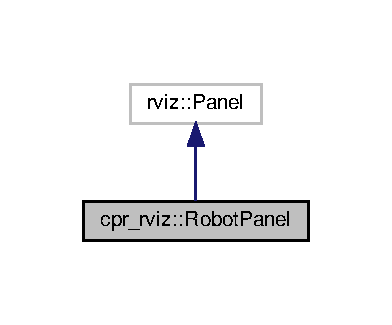
\includegraphics[width=188pt]{classcpr__rviz_1_1RobotPanel__inherit__graph}
\end{center}
\end{figure}
\subsection*{Public Member Functions}
\begin{DoxyCompactItemize}
\item 
\textbf{ Robot\+Panel} (Q\+Widget $\ast$parent=nullptr)
\begin{DoxyCompactList}\small\item\em Constructor of the \doxyref{Robot\+Panel}{p.}{classcpr__rviz_1_1RobotPanel} class. \end{DoxyCompactList}\item 
virtual \textbf{ $\sim$\+Robot\+Panel} ()
\begin{DoxyCompactList}\small\item\em Destructor of the \doxyref{Robot\+Panel}{p.}{classcpr__rviz_1_1RobotPanel} class. \end{DoxyCompactList}\end{DoxyCompactItemize}
\subsection*{Protected Slots}
\begin{DoxyCompactItemize}
\item 
void \textbf{ On\+Connect\+Button\+Clicked} (bool b\+Checked=true)
\begin{DoxyCompactList}\small\item\em Callback slot handling clicks to the \char`\"{}\+Connect/\+Disconnect\char`\"{} button. \end{DoxyCompactList}\item 
void \textbf{ On\+Enable\+Button\+Clicked} (bool b\+Checked=true)
\begin{DoxyCompactList}\small\item\em Callback slot handling clicks to the \char`\"{}\+Enable/\+Disable\char`\"{} button. \end{DoxyCompactList}\item 
void \textbf{ On\+Override\+Slider\+Value\+Changed} (int value)
\begin{DoxyCompactList}\small\item\em Callback slot handling changes to the override slider value. \end{DoxyCompactList}\item 
void \textbf{ On\+Reference\+Button\+Clicked} (bool b\+Checked=true)
\begin{DoxyCompactList}\small\item\em Callback slot handling clicks to the \char`\"{}\+Reference\char`\"{} button. \end{DoxyCompactList}\item 
void \textbf{ On\+Zero\+Button\+Clicked} (bool b\+Checked=true)
\begin{DoxyCompactList}\small\item\em Callback slot handling clicks to the \char`\"{}\+Set Zero\char`\"{} button. \end{DoxyCompactList}\end{DoxyCompactItemize}
\subsection*{Protected Member Functions}
\begin{DoxyCompactItemize}
\item 
cpr\+\_\+robot\+::\+Get\+Robot\+Info\+Response \textbf{ Get\+Robot\+Info} ()
\begin{DoxyCompactList}\small\item\em Queries information about the robot from the /\+Get\+Robot\+Info R\+OS service. \end{DoxyCompactList}\item 
cpr\+\_\+robot\+::\+Robot\+Command\+Response \textbf{ Robot\+Command} (const uint32\+\_\+t command\+Id, const double payload\+Float, const int64\+\_\+t payload\+Int)
\begin{DoxyCompactList}\small\item\em Sends a command to the robot using the /\+Robot\+Command R\+OS service. \end{DoxyCompactList}\end{DoxyCompactItemize}
\subsection*{Private Member Functions}
\begin{DoxyCompactItemize}
\item 
void \textbf{ Initialize\+R\+OS} ()
\begin{DoxyCompactList}\small\item\em Sets up communication with R\+OS. \end{DoxyCompactList}\item 
void \textbf{ Initialize\+State} ()
\begin{DoxyCompactList}\small\item\em Initializes all relevant members. \end{DoxyCompactList}\item 
void \textbf{ Initialize\+UI} ()
\begin{DoxyCompactList}\small\item\em Initializes all relevant UI elements. \end{DoxyCompactList}\item 
void \textbf{ On\+Override\+Changed} ()
\begin{DoxyCompactList}\small\item\em Updates all UI elements associated with the override value of the robot. \end{DoxyCompactList}\item 
void \textbf{ On\+Status\+Flags\+Changed} ()
\begin{DoxyCompactList}\small\item\em Updates all UI elements associated with the status flag reported by the robot. \end{DoxyCompactList}\item 
void \textbf{ Robot\+State\+Callback} (const cpr\+\_\+robot\+::\+Robot\+State\+::\+Const\+Ptr \&msg)
\begin{DoxyCompactList}\small\item\em Callback that handles messages received over the /\+Robot\+State R\+OS topic. \end{DoxyCompactList}\end{DoxyCompactItemize}
\subsection*{Private Attributes}
\begin{DoxyCompactItemize}
\item 
Q\+Push\+Button \textbf{ m\+\_\+\+Connect\+Button}
\begin{DoxyCompactList}\small\item\em Button allowing to connect/disconnect the robot remotely. \end{DoxyCompactList}\item 
Q\+H\+Box\+Layout \textbf{ m\+\_\+\+Control\+Buttons\+Layout}
\begin{DoxyCompactList}\small\item\em Layout aranging the control buttons horizontally. \end{DoxyCompactList}\item 
uint32\+\_\+t \textbf{ m\+\_\+\+Count\+Joints}
\begin{DoxyCompactList}\small\item\em The number of joints reported by the robot. \end{DoxyCompactList}\item 
Q\+Push\+Button \textbf{ m\+\_\+\+Enable\+Button}
\begin{DoxyCompactList}\small\item\em Button allowing to enable/disable motor motion on the robot remotely. \end{DoxyCompactList}\item 
ros\+::\+Service\+Client \textbf{ m\+\_\+\+Get\+Robot\+Info\+Client}
\begin{DoxyCompactList}\small\item\em Client used to query information about the robot via the /\+Get\+Robot\+Info R\+OS service. \end{DoxyCompactList}\item 
Q\+Grid\+Layout \textbf{ m\+\_\+\+Joints\+Layout}
\begin{DoxyCompactList}\small\item\em Layout arranging the controls of the individual joints. \end{DoxyCompactList}\item 
Q\+Form\+Layout \textbf{ m\+\_\+\+Main\+Layout}
\begin{DoxyCompactList}\small\item\em The top-\/level layout of this widget. \end{DoxyCompactList}\item 
std\+::string \textbf{ m\+\_\+\+Model\+Name}
\begin{DoxyCompactList}\small\item\em The model designation reported by the robot. \end{DoxyCompactList}\item 
Q\+Label \textbf{ m\+\_\+\+Model\+Name\+Label}
\begin{DoxyCompactList}\small\item\em Label used to show the model deisgnation of the robot. \end{DoxyCompactList}\item 
ros\+::\+Node\+Handle \textbf{ m\+\_\+\+Node}
\begin{DoxyCompactList}\small\item\em A handle to the current R\+OS node. \end{DoxyCompactList}\item 
double \textbf{ m\+\_\+\+Override}
\begin{DoxyCompactList}\small\item\em The override value reported by the robot. \end{DoxyCompactList}\item 
Q\+Label \textbf{ m\+\_\+\+Override\+Label}
\begin{DoxyCompactList}\small\item\em Label used to show the current override value of the robot. \end{DoxyCompactList}\item 
Q\+Slider \textbf{ m\+\_\+\+Override\+Slider}
\begin{DoxyCompactList}\small\item\em Slider used to change the desired override value of the robot. \end{DoxyCompactList}\item 
bool \textbf{ m\+\_\+\+Override\+Slider\+Valid}
\begin{DoxyCompactList}\small\item\em Flag indicating whether the position of the override slider has been properly initialized. \end{DoxyCompactList}\item 
\textbf{ Joint\+Control} $\ast$$\ast$ \textbf{ m\+\_\+p\+Joint\+Controls}
\begin{DoxyCompactList}\small\item\em Array containing the control widgets for the individual joints. \end{DoxyCompactList}\item 
Q\+Push\+Button \textbf{ m\+\_\+\+Reference\+Button}
\begin{DoxyCompactList}\small\item\em Button allowing to start the referencing procedure on the robot remotely. \end{DoxyCompactList}\item 
ros\+::\+Service\+Client \textbf{ m\+\_\+\+Robot\+Command\+Client}
\begin{DoxyCompactList}\small\item\em Client used to send commands to the robot via the /\+Robot\+Command R\+OS service. \end{DoxyCompactList}\item 
ros\+::\+Subscriber \textbf{ m\+\_\+\+Robot\+State\+Subscriber}
\begin{DoxyCompactList}\small\item\em Subscriber listening to the /\+Robot\+State R\+OS topic. \end{DoxyCompactList}\item 
uint32\+\_\+t \textbf{ m\+\_\+\+Status\+Flags}
\begin{DoxyCompactList}\small\item\em The status flags reported by the robot. \end{DoxyCompactList}\item 
Q\+Push\+Button \textbf{ m\+\_\+\+Zero\+Button}
\begin{DoxyCompactList}\small\item\em Button allowing to set the encoder positions on the robot remotely to zero. \end{DoxyCompactList}\end{DoxyCompactItemize}


\subsection{Detailed Description}
Plugin for R\+Viz that allows to move a robot remotely over R\+OS. 

Definition at line 7 of file Robot\+Panel.\+h.



\subsection{Constructor \& Destructor Documentation}
\mbox{\label{classcpr__rviz_1_1RobotPanel_a94a53fc745942210d8eac594618a7ef6}} 
\index{cpr\+\_\+rviz\+::\+Robot\+Panel@{cpr\+\_\+rviz\+::\+Robot\+Panel}!Robot\+Panel@{Robot\+Panel}}
\index{Robot\+Panel@{Robot\+Panel}!cpr\+\_\+rviz\+::\+Robot\+Panel@{cpr\+\_\+rviz\+::\+Robot\+Panel}}
\subsubsection{Robot\+Panel()}
{\footnotesize\ttfamily cpr\+\_\+rviz\+::\+Robot\+Panel\+::\+Robot\+Panel (\begin{DoxyParamCaption}\item[{Q\+Widget $\ast$}]{parent = {\ttfamily nullptr} }\end{DoxyParamCaption})}



Constructor of the \doxyref{Robot\+Panel}{p.}{classcpr__rviz_1_1RobotPanel} class. 


\begin{DoxyParams}{Parameters}
{\em parent} & The parent widget. \\
\hline
\end{DoxyParams}


Definition at line 11 of file Robot\+Panel.\+cpp.

\mbox{\label{classcpr__rviz_1_1RobotPanel_a58e5efe4432a01954808a97a4c55bd43}} 
\index{cpr\+\_\+rviz\+::\+Robot\+Panel@{cpr\+\_\+rviz\+::\+Robot\+Panel}!````~Robot\+Panel@{$\sim$\+Robot\+Panel}}
\index{````~Robot\+Panel@{$\sim$\+Robot\+Panel}!cpr\+\_\+rviz\+::\+Robot\+Panel@{cpr\+\_\+rviz\+::\+Robot\+Panel}}
\subsubsection{$\sim$\+Robot\+Panel()}
{\footnotesize\ttfamily cpr\+\_\+rviz\+::\+Robot\+Panel\+::$\sim$\+Robot\+Panel (\begin{DoxyParamCaption}{ }\end{DoxyParamCaption})\hspace{0.3cm}{\ttfamily [virtual]}}



Destructor of the \doxyref{Robot\+Panel}{p.}{classcpr__rviz_1_1RobotPanel} class. 



Definition at line 27 of file Robot\+Panel.\+cpp.



\subsection{Member Function Documentation}
\mbox{\label{classcpr__rviz_1_1RobotPanel_a8df43a1e1dd42263657df7202f8bdf3c}} 
\index{cpr\+\_\+rviz\+::\+Robot\+Panel@{cpr\+\_\+rviz\+::\+Robot\+Panel}!Get\+Robot\+Info@{Get\+Robot\+Info}}
\index{Get\+Robot\+Info@{Get\+Robot\+Info}!cpr\+\_\+rviz\+::\+Robot\+Panel@{cpr\+\_\+rviz\+::\+Robot\+Panel}}
\subsubsection{Get\+Robot\+Info()}
{\footnotesize\ttfamily cpr\+\_\+robot\+::\+Get\+Robot\+Info\+Response cpr\+\_\+rviz\+::\+Robot\+Panel\+::\+Get\+Robot\+Info (\begin{DoxyParamCaption}{ }\end{DoxyParamCaption})\hspace{0.3cm}{\ttfamily [protected]}}



Queries information about the robot from the /\+Get\+Robot\+Info R\+OS service. 



Definition at line 204 of file Robot\+Panel.\+cpp.

\mbox{\label{classcpr__rviz_1_1RobotPanel_a89d390543160974edfa948a0c8fb232d}} 
\index{cpr\+\_\+rviz\+::\+Robot\+Panel@{cpr\+\_\+rviz\+::\+Robot\+Panel}!Initialize\+R\+OS@{Initialize\+R\+OS}}
\index{Initialize\+R\+OS@{Initialize\+R\+OS}!cpr\+\_\+rviz\+::\+Robot\+Panel@{cpr\+\_\+rviz\+::\+Robot\+Panel}}
\subsubsection{Initialize\+R\+O\+S()}
{\footnotesize\ttfamily void cpr\+\_\+rviz\+::\+Robot\+Panel\+::\+Initialize\+R\+OS (\begin{DoxyParamCaption}{ }\end{DoxyParamCaption})\hspace{0.3cm}{\ttfamily [private]}}



Sets up communication with R\+OS. 



Definition at line 120 of file Robot\+Panel.\+cpp.

\mbox{\label{classcpr__rviz_1_1RobotPanel_a2677e67d3eb7adf335958f21c3f7f653}} 
\index{cpr\+\_\+rviz\+::\+Robot\+Panel@{cpr\+\_\+rviz\+::\+Robot\+Panel}!Initialize\+State@{Initialize\+State}}
\index{Initialize\+State@{Initialize\+State}!cpr\+\_\+rviz\+::\+Robot\+Panel@{cpr\+\_\+rviz\+::\+Robot\+Panel}}
\subsubsection{Initialize\+State()}
{\footnotesize\ttfamily void cpr\+\_\+rviz\+::\+Robot\+Panel\+::\+Initialize\+State (\begin{DoxyParamCaption}{ }\end{DoxyParamCaption})\hspace{0.3cm}{\ttfamily [private]}}



Initializes all relevant members. 



Definition at line 111 of file Robot\+Panel.\+cpp.

\mbox{\label{classcpr__rviz_1_1RobotPanel_af1a8e718388e371a1b3d380353853431}} 
\index{cpr\+\_\+rviz\+::\+Robot\+Panel@{cpr\+\_\+rviz\+::\+Robot\+Panel}!Initialize\+UI@{Initialize\+UI}}
\index{Initialize\+UI@{Initialize\+UI}!cpr\+\_\+rviz\+::\+Robot\+Panel@{cpr\+\_\+rviz\+::\+Robot\+Panel}}
\subsubsection{Initialize\+U\+I()}
{\footnotesize\ttfamily void cpr\+\_\+rviz\+::\+Robot\+Panel\+::\+Initialize\+UI (\begin{DoxyParamCaption}{ }\end{DoxyParamCaption})\hspace{0.3cm}{\ttfamily [private]}}



Initializes all relevant UI elements. 



Definition at line 39 of file Robot\+Panel.\+cpp.

\mbox{\label{classcpr__rviz_1_1RobotPanel_aab90d125fdb7f2eedd8f369dbe260fe5}} 
\index{cpr\+\_\+rviz\+::\+Robot\+Panel@{cpr\+\_\+rviz\+::\+Robot\+Panel}!On\+Connect\+Button\+Clicked@{On\+Connect\+Button\+Clicked}}
\index{On\+Connect\+Button\+Clicked@{On\+Connect\+Button\+Clicked}!cpr\+\_\+rviz\+::\+Robot\+Panel@{cpr\+\_\+rviz\+::\+Robot\+Panel}}
\subsubsection{On\+Connect\+Button\+Clicked}
{\footnotesize\ttfamily void cpr\+\_\+rviz\+::\+Robot\+Panel\+::\+On\+Connect\+Button\+Clicked (\begin{DoxyParamCaption}\item[{bool}]{b\+Checked = {\ttfamily true} }\end{DoxyParamCaption})\hspace{0.3cm}{\ttfamily [protected]}, {\ttfamily [slot]}}



Callback slot handling clicks to the \char`\"{}\+Connect/\+Disconnect\char`\"{} button. 



Definition at line 81 of file Robot\+Panel.\+cpp.

\mbox{\label{classcpr__rviz_1_1RobotPanel_a95658f429ca681929ee72af87f62ce94}} 
\index{cpr\+\_\+rviz\+::\+Robot\+Panel@{cpr\+\_\+rviz\+::\+Robot\+Panel}!On\+Enable\+Button\+Clicked@{On\+Enable\+Button\+Clicked}}
\index{On\+Enable\+Button\+Clicked@{On\+Enable\+Button\+Clicked}!cpr\+\_\+rviz\+::\+Robot\+Panel@{cpr\+\_\+rviz\+::\+Robot\+Panel}}
\subsubsection{On\+Enable\+Button\+Clicked}
{\footnotesize\ttfamily void cpr\+\_\+rviz\+::\+Robot\+Panel\+::\+On\+Enable\+Button\+Clicked (\begin{DoxyParamCaption}\item[{bool}]{b\+Checked = {\ttfamily true} }\end{DoxyParamCaption})\hspace{0.3cm}{\ttfamily [protected]}, {\ttfamily [slot]}}



Callback slot handling clicks to the \char`\"{}\+Enable/\+Disable\char`\"{} button. 



Definition at line 102 of file Robot\+Panel.\+cpp.

\mbox{\label{classcpr__rviz_1_1RobotPanel_a7e371cd8ca1aa26eef82c61ddaa93a7b}} 
\index{cpr\+\_\+rviz\+::\+Robot\+Panel@{cpr\+\_\+rviz\+::\+Robot\+Panel}!On\+Override\+Changed@{On\+Override\+Changed}}
\index{On\+Override\+Changed@{On\+Override\+Changed}!cpr\+\_\+rviz\+::\+Robot\+Panel@{cpr\+\_\+rviz\+::\+Robot\+Panel}}
\subsubsection{On\+Override\+Changed()}
{\footnotesize\ttfamily void cpr\+\_\+rviz\+::\+Robot\+Panel\+::\+On\+Override\+Changed (\begin{DoxyParamCaption}{ }\end{DoxyParamCaption})\hspace{0.3cm}{\ttfamily [private]}}



Updates all UI elements associated with the override value of the robot. 



Definition at line 160 of file Robot\+Panel.\+cpp.

\mbox{\label{classcpr__rviz_1_1RobotPanel_ac1672149b82d5e09d4a6337021cca43d}} 
\index{cpr\+\_\+rviz\+::\+Robot\+Panel@{cpr\+\_\+rviz\+::\+Robot\+Panel}!On\+Override\+Slider\+Value\+Changed@{On\+Override\+Slider\+Value\+Changed}}
\index{On\+Override\+Slider\+Value\+Changed@{On\+Override\+Slider\+Value\+Changed}!cpr\+\_\+rviz\+::\+Robot\+Panel@{cpr\+\_\+rviz\+::\+Robot\+Panel}}
\subsubsection{On\+Override\+Slider\+Value\+Changed}
{\footnotesize\ttfamily void cpr\+\_\+rviz\+::\+Robot\+Panel\+::\+On\+Override\+Slider\+Value\+Changed (\begin{DoxyParamCaption}\item[{int}]{value }\end{DoxyParamCaption})\hspace{0.3cm}{\ttfamily [protected]}, {\ttfamily [slot]}}



Callback slot handling changes to the override slider value. 



Definition at line 75 of file Robot\+Panel.\+cpp.

\mbox{\label{classcpr__rviz_1_1RobotPanel_ae959eae9146d9d3531217ff35bc5fb18}} 
\index{cpr\+\_\+rviz\+::\+Robot\+Panel@{cpr\+\_\+rviz\+::\+Robot\+Panel}!On\+Reference\+Button\+Clicked@{On\+Reference\+Button\+Clicked}}
\index{On\+Reference\+Button\+Clicked@{On\+Reference\+Button\+Clicked}!cpr\+\_\+rviz\+::\+Robot\+Panel@{cpr\+\_\+rviz\+::\+Robot\+Panel}}
\subsubsection{On\+Reference\+Button\+Clicked}
{\footnotesize\ttfamily void cpr\+\_\+rviz\+::\+Robot\+Panel\+::\+On\+Reference\+Button\+Clicked (\begin{DoxyParamCaption}\item[{bool}]{b\+Checked = {\ttfamily true} }\end{DoxyParamCaption})\hspace{0.3cm}{\ttfamily [protected]}, {\ttfamily [slot]}}



Callback slot handling clicks to the \char`\"{}\+Reference\char`\"{} button. 



Definition at line 90 of file Robot\+Panel.\+cpp.

\mbox{\label{classcpr__rviz_1_1RobotPanel_aa019eb59585e0f1d31ff621367be775a}} 
\index{cpr\+\_\+rviz\+::\+Robot\+Panel@{cpr\+\_\+rviz\+::\+Robot\+Panel}!On\+Status\+Flags\+Changed@{On\+Status\+Flags\+Changed}}
\index{On\+Status\+Flags\+Changed@{On\+Status\+Flags\+Changed}!cpr\+\_\+rviz\+::\+Robot\+Panel@{cpr\+\_\+rviz\+::\+Robot\+Panel}}
\subsubsection{On\+Status\+Flags\+Changed()}
{\footnotesize\ttfamily void cpr\+\_\+rviz\+::\+Robot\+Panel\+::\+On\+Status\+Flags\+Changed (\begin{DoxyParamCaption}{ }\end{DoxyParamCaption})\hspace{0.3cm}{\ttfamily [private]}}



Updates all UI elements associated with the status flag reported by the robot. 



Definition at line 168 of file Robot\+Panel.\+cpp.

\mbox{\label{classcpr__rviz_1_1RobotPanel_a11c94355f7de5648f010fbaf33a91a5d}} 
\index{cpr\+\_\+rviz\+::\+Robot\+Panel@{cpr\+\_\+rviz\+::\+Robot\+Panel}!On\+Zero\+Button\+Clicked@{On\+Zero\+Button\+Clicked}}
\index{On\+Zero\+Button\+Clicked@{On\+Zero\+Button\+Clicked}!cpr\+\_\+rviz\+::\+Robot\+Panel@{cpr\+\_\+rviz\+::\+Robot\+Panel}}
\subsubsection{On\+Zero\+Button\+Clicked}
{\footnotesize\ttfamily void cpr\+\_\+rviz\+::\+Robot\+Panel\+::\+On\+Zero\+Button\+Clicked (\begin{DoxyParamCaption}\item[{bool}]{b\+Checked = {\ttfamily true} }\end{DoxyParamCaption})\hspace{0.3cm}{\ttfamily [protected]}, {\ttfamily [slot]}}



Callback slot handling clicks to the \char`\"{}\+Set Zero\char`\"{} button. 



Definition at line 96 of file Robot\+Panel.\+cpp.

\mbox{\label{classcpr__rviz_1_1RobotPanel_a80ddb6e75b38c08a8cf9cf2df5129447}} 
\index{cpr\+\_\+rviz\+::\+Robot\+Panel@{cpr\+\_\+rviz\+::\+Robot\+Panel}!Robot\+Command@{Robot\+Command}}
\index{Robot\+Command@{Robot\+Command}!cpr\+\_\+rviz\+::\+Robot\+Panel@{cpr\+\_\+rviz\+::\+Robot\+Panel}}
\subsubsection{Robot\+Command()}
{\footnotesize\ttfamily cpr\+\_\+robot\+::\+Robot\+Command\+Response cpr\+\_\+rviz\+::\+Robot\+Panel\+::\+Robot\+Command (\begin{DoxyParamCaption}\item[{const uint32\+\_\+t}]{command\+Id,  }\item[{const double}]{payload\+Float,  }\item[{const int64\+\_\+t}]{payload\+Int }\end{DoxyParamCaption})\hspace{0.3cm}{\ttfamily [protected]}}



Sends a command to the robot using the /\+Robot\+Command R\+OS service. 


\begin{DoxyParams}{Parameters}
{\em command\+Id} & The ID of the command that will be sent. \\
\hline
{\em payload\+Float} & A floating point number that may be provided as data with the command. \\
\hline
{\em payload\+Int} & An integer number that may be provided as data with the command. \\
\hline
\end{DoxyParams}


Definition at line 225 of file Robot\+Panel.\+cpp.

\mbox{\label{classcpr__rviz_1_1RobotPanel_a319077ba01379334cfcf1393d9dfeb9b}} 
\index{cpr\+\_\+rviz\+::\+Robot\+Panel@{cpr\+\_\+rviz\+::\+Robot\+Panel}!Robot\+State\+Callback@{Robot\+State\+Callback}}
\index{Robot\+State\+Callback@{Robot\+State\+Callback}!cpr\+\_\+rviz\+::\+Robot\+Panel@{cpr\+\_\+rviz\+::\+Robot\+Panel}}
\subsubsection{Robot\+State\+Callback()}
{\footnotesize\ttfamily void cpr\+\_\+rviz\+::\+Robot\+Panel\+::\+Robot\+State\+Callback (\begin{DoxyParamCaption}\item[{const cpr\+\_\+robot\+::\+Robot\+State\+::\+Const\+Ptr \&}]{msg }\end{DoxyParamCaption})\hspace{0.3cm}{\ttfamily [private]}}



Callback that handles messages received over the /\+Robot\+State R\+OS topic. 


\begin{DoxyParams}{Parameters}
{\em msg} & The received message. \\
\hline
\end{DoxyParams}


Definition at line 129 of file Robot\+Panel.\+cpp.



\subsection{Member Data Documentation}
\mbox{\label{classcpr__rviz_1_1RobotPanel_a4f0750b3996001ff45e8610b07d690cc}} 
\index{cpr\+\_\+rviz\+::\+Robot\+Panel@{cpr\+\_\+rviz\+::\+Robot\+Panel}!m\+\_\+\+Connect\+Button@{m\+\_\+\+Connect\+Button}}
\index{m\+\_\+\+Connect\+Button@{m\+\_\+\+Connect\+Button}!cpr\+\_\+rviz\+::\+Robot\+Panel@{cpr\+\_\+rviz\+::\+Robot\+Panel}}
\subsubsection{m\+\_\+\+Connect\+Button}
{\footnotesize\ttfamily Q\+Push\+Button cpr\+\_\+rviz\+::\+Robot\+Panel\+::m\+\_\+\+Connect\+Button\hspace{0.3cm}{\ttfamily [private]}}



Button allowing to connect/disconnect the robot remotely. 



Definition at line 26 of file Robot\+Panel.\+h.

\mbox{\label{classcpr__rviz_1_1RobotPanel_a1acad3f0f8f1a0fc684774c2aba7ed2b}} 
\index{cpr\+\_\+rviz\+::\+Robot\+Panel@{cpr\+\_\+rviz\+::\+Robot\+Panel}!m\+\_\+\+Control\+Buttons\+Layout@{m\+\_\+\+Control\+Buttons\+Layout}}
\index{m\+\_\+\+Control\+Buttons\+Layout@{m\+\_\+\+Control\+Buttons\+Layout}!cpr\+\_\+rviz\+::\+Robot\+Panel@{cpr\+\_\+rviz\+::\+Robot\+Panel}}
\subsubsection{m\+\_\+\+Control\+Buttons\+Layout}
{\footnotesize\ttfamily Q\+H\+Box\+Layout cpr\+\_\+rviz\+::\+Robot\+Panel\+::m\+\_\+\+Control\+Buttons\+Layout\hspace{0.3cm}{\ttfamily [private]}}



Layout aranging the control buttons horizontally. 



Definition at line 24 of file Robot\+Panel.\+h.

\mbox{\label{classcpr__rviz_1_1RobotPanel_aa00028789ad9fa3d1cf2655f1c64a71e}} 
\index{cpr\+\_\+rviz\+::\+Robot\+Panel@{cpr\+\_\+rviz\+::\+Robot\+Panel}!m\+\_\+\+Count\+Joints@{m\+\_\+\+Count\+Joints}}
\index{m\+\_\+\+Count\+Joints@{m\+\_\+\+Count\+Joints}!cpr\+\_\+rviz\+::\+Robot\+Panel@{cpr\+\_\+rviz\+::\+Robot\+Panel}}
\subsubsection{m\+\_\+\+Count\+Joints}
{\footnotesize\ttfamily uint32\+\_\+t cpr\+\_\+rviz\+::\+Robot\+Panel\+::m\+\_\+\+Count\+Joints\hspace{0.3cm}{\ttfamily [private]}}



The number of joints reported by the robot. 



Definition at line 22 of file Robot\+Panel.\+h.

\mbox{\label{classcpr__rviz_1_1RobotPanel_a2b4b61e1c1c776afe520113e1809db81}} 
\index{cpr\+\_\+rviz\+::\+Robot\+Panel@{cpr\+\_\+rviz\+::\+Robot\+Panel}!m\+\_\+\+Enable\+Button@{m\+\_\+\+Enable\+Button}}
\index{m\+\_\+\+Enable\+Button@{m\+\_\+\+Enable\+Button}!cpr\+\_\+rviz\+::\+Robot\+Panel@{cpr\+\_\+rviz\+::\+Robot\+Panel}}
\subsubsection{m\+\_\+\+Enable\+Button}
{\footnotesize\ttfamily Q\+Push\+Button cpr\+\_\+rviz\+::\+Robot\+Panel\+::m\+\_\+\+Enable\+Button\hspace{0.3cm}{\ttfamily [private]}}



Button allowing to enable/disable motor motion on the robot remotely. 



Definition at line 28 of file Robot\+Panel.\+h.

\mbox{\label{classcpr__rviz_1_1RobotPanel_aed4833783aa8e0d18f951c356924b8d4}} 
\index{cpr\+\_\+rviz\+::\+Robot\+Panel@{cpr\+\_\+rviz\+::\+Robot\+Panel}!m\+\_\+\+Get\+Robot\+Info\+Client@{m\+\_\+\+Get\+Robot\+Info\+Client}}
\index{m\+\_\+\+Get\+Robot\+Info\+Client@{m\+\_\+\+Get\+Robot\+Info\+Client}!cpr\+\_\+rviz\+::\+Robot\+Panel@{cpr\+\_\+rviz\+::\+Robot\+Panel}}
\subsubsection{m\+\_\+\+Get\+Robot\+Info\+Client}
{\footnotesize\ttfamily ros\+::\+Service\+Client cpr\+\_\+rviz\+::\+Robot\+Panel\+::m\+\_\+\+Get\+Robot\+Info\+Client\hspace{0.3cm}{\ttfamily [private]}}



Client used to query information about the robot via the /\+Get\+Robot\+Info R\+OS service. 



Definition at line 14 of file Robot\+Panel.\+h.

\mbox{\label{classcpr__rviz_1_1RobotPanel_ae61c2afa8026071af8505de5445e74f7}} 
\index{cpr\+\_\+rviz\+::\+Robot\+Panel@{cpr\+\_\+rviz\+::\+Robot\+Panel}!m\+\_\+\+Joints\+Layout@{m\+\_\+\+Joints\+Layout}}
\index{m\+\_\+\+Joints\+Layout@{m\+\_\+\+Joints\+Layout}!cpr\+\_\+rviz\+::\+Robot\+Panel@{cpr\+\_\+rviz\+::\+Robot\+Panel}}
\subsubsection{m\+\_\+\+Joints\+Layout}
{\footnotesize\ttfamily Q\+Grid\+Layout cpr\+\_\+rviz\+::\+Robot\+Panel\+::m\+\_\+\+Joints\+Layout\hspace{0.3cm}{\ttfamily [private]}}



Layout arranging the controls of the individual joints. 



Definition at line 38 of file Robot\+Panel.\+h.

\mbox{\label{classcpr__rviz_1_1RobotPanel_a28932ab9c394aac8c5b6fe182e6ffa2c}} 
\index{cpr\+\_\+rviz\+::\+Robot\+Panel@{cpr\+\_\+rviz\+::\+Robot\+Panel}!m\+\_\+\+Main\+Layout@{m\+\_\+\+Main\+Layout}}
\index{m\+\_\+\+Main\+Layout@{m\+\_\+\+Main\+Layout}!cpr\+\_\+rviz\+::\+Robot\+Panel@{cpr\+\_\+rviz\+::\+Robot\+Panel}}
\subsubsection{m\+\_\+\+Main\+Layout}
{\footnotesize\ttfamily Q\+Form\+Layout cpr\+\_\+rviz\+::\+Robot\+Panel\+::m\+\_\+\+Main\+Layout\hspace{0.3cm}{\ttfamily [private]}}



The top-\/level layout of this widget. 



Definition at line 40 of file Robot\+Panel.\+h.

\mbox{\label{classcpr__rviz_1_1RobotPanel_ac08e77be9ef4ef89af6126bb9a0e3288}} 
\index{cpr\+\_\+rviz\+::\+Robot\+Panel@{cpr\+\_\+rviz\+::\+Robot\+Panel}!m\+\_\+\+Model\+Name@{m\+\_\+\+Model\+Name}}
\index{m\+\_\+\+Model\+Name@{m\+\_\+\+Model\+Name}!cpr\+\_\+rviz\+::\+Robot\+Panel@{cpr\+\_\+rviz\+::\+Robot\+Panel}}
\subsubsection{m\+\_\+\+Model\+Name}
{\footnotesize\ttfamily std\+::string cpr\+\_\+rviz\+::\+Robot\+Panel\+::m\+\_\+\+Model\+Name\hspace{0.3cm}{\ttfamily [private]}}



The model designation reported by the robot. 



Definition at line 20 of file Robot\+Panel.\+h.

\mbox{\label{classcpr__rviz_1_1RobotPanel_af18da4751b3bea874ded23126bdede64}} 
\index{cpr\+\_\+rviz\+::\+Robot\+Panel@{cpr\+\_\+rviz\+::\+Robot\+Panel}!m\+\_\+\+Model\+Name\+Label@{m\+\_\+\+Model\+Name\+Label}}
\index{m\+\_\+\+Model\+Name\+Label@{m\+\_\+\+Model\+Name\+Label}!cpr\+\_\+rviz\+::\+Robot\+Panel@{cpr\+\_\+rviz\+::\+Robot\+Panel}}
\subsubsection{m\+\_\+\+Model\+Name\+Label}
{\footnotesize\ttfamily Q\+Label cpr\+\_\+rviz\+::\+Robot\+Panel\+::m\+\_\+\+Model\+Name\+Label\hspace{0.3cm}{\ttfamily [private]}}



Label used to show the model deisgnation of the robot. 



Definition at line 42 of file Robot\+Panel.\+h.

\mbox{\label{classcpr__rviz_1_1RobotPanel_a6978e66039178ef430787b5852518537}} 
\index{cpr\+\_\+rviz\+::\+Robot\+Panel@{cpr\+\_\+rviz\+::\+Robot\+Panel}!m\+\_\+\+Node@{m\+\_\+\+Node}}
\index{m\+\_\+\+Node@{m\+\_\+\+Node}!cpr\+\_\+rviz\+::\+Robot\+Panel@{cpr\+\_\+rviz\+::\+Robot\+Panel}}
\subsubsection{m\+\_\+\+Node}
{\footnotesize\ttfamily ros\+::\+Node\+Handle cpr\+\_\+rviz\+::\+Robot\+Panel\+::m\+\_\+\+Node\hspace{0.3cm}{\ttfamily [private]}}



A handle to the current R\+OS node. 



Definition at line 12 of file Robot\+Panel.\+h.

\mbox{\label{classcpr__rviz_1_1RobotPanel_aa002130e0ac251ab17271ae66f756869}} 
\index{cpr\+\_\+rviz\+::\+Robot\+Panel@{cpr\+\_\+rviz\+::\+Robot\+Panel}!m\+\_\+\+Override@{m\+\_\+\+Override}}
\index{m\+\_\+\+Override@{m\+\_\+\+Override}!cpr\+\_\+rviz\+::\+Robot\+Panel@{cpr\+\_\+rviz\+::\+Robot\+Panel}}
\subsubsection{m\+\_\+\+Override}
{\footnotesize\ttfamily double cpr\+\_\+rviz\+::\+Robot\+Panel\+::m\+\_\+\+Override\hspace{0.3cm}{\ttfamily [private]}}



The override value reported by the robot. 



Definition at line 46 of file Robot\+Panel.\+h.

\mbox{\label{classcpr__rviz_1_1RobotPanel_a7a5b969e1b67121ad22514e92cd1df60}} 
\index{cpr\+\_\+rviz\+::\+Robot\+Panel@{cpr\+\_\+rviz\+::\+Robot\+Panel}!m\+\_\+\+Override\+Label@{m\+\_\+\+Override\+Label}}
\index{m\+\_\+\+Override\+Label@{m\+\_\+\+Override\+Label}!cpr\+\_\+rviz\+::\+Robot\+Panel@{cpr\+\_\+rviz\+::\+Robot\+Panel}}
\subsubsection{m\+\_\+\+Override\+Label}
{\footnotesize\ttfamily Q\+Label cpr\+\_\+rviz\+::\+Robot\+Panel\+::m\+\_\+\+Override\+Label\hspace{0.3cm}{\ttfamily [private]}}



Label used to show the current override value of the robot. 



Definition at line 34 of file Robot\+Panel.\+h.

\mbox{\label{classcpr__rviz_1_1RobotPanel_a7f821beda431c95e824d8bc3934fd5e5}} 
\index{cpr\+\_\+rviz\+::\+Robot\+Panel@{cpr\+\_\+rviz\+::\+Robot\+Panel}!m\+\_\+\+Override\+Slider@{m\+\_\+\+Override\+Slider}}
\index{m\+\_\+\+Override\+Slider@{m\+\_\+\+Override\+Slider}!cpr\+\_\+rviz\+::\+Robot\+Panel@{cpr\+\_\+rviz\+::\+Robot\+Panel}}
\subsubsection{m\+\_\+\+Override\+Slider}
{\footnotesize\ttfamily Q\+Slider cpr\+\_\+rviz\+::\+Robot\+Panel\+::m\+\_\+\+Override\+Slider\hspace{0.3cm}{\ttfamily [private]}}



Slider used to change the desired override value of the robot. 



Definition at line 36 of file Robot\+Panel.\+h.

\mbox{\label{classcpr__rviz_1_1RobotPanel_a6561d3845bb6ebd5bb88de2734c0b490}} 
\index{cpr\+\_\+rviz\+::\+Robot\+Panel@{cpr\+\_\+rviz\+::\+Robot\+Panel}!m\+\_\+\+Override\+Slider\+Valid@{m\+\_\+\+Override\+Slider\+Valid}}
\index{m\+\_\+\+Override\+Slider\+Valid@{m\+\_\+\+Override\+Slider\+Valid}!cpr\+\_\+rviz\+::\+Robot\+Panel@{cpr\+\_\+rviz\+::\+Robot\+Panel}}
\subsubsection{m\+\_\+\+Override\+Slider\+Valid}
{\footnotesize\ttfamily bool cpr\+\_\+rviz\+::\+Robot\+Panel\+::m\+\_\+\+Override\+Slider\+Valid\hspace{0.3cm}{\ttfamily [private]}}



Flag indicating whether the position of the override slider has been properly initialized. 



Definition at line 48 of file Robot\+Panel.\+h.

\mbox{\label{classcpr__rviz_1_1RobotPanel_ade7adfc4817b469b83e64d45ae39c806}} 
\index{cpr\+\_\+rviz\+::\+Robot\+Panel@{cpr\+\_\+rviz\+::\+Robot\+Panel}!m\+\_\+p\+Joint\+Controls@{m\+\_\+p\+Joint\+Controls}}
\index{m\+\_\+p\+Joint\+Controls@{m\+\_\+p\+Joint\+Controls}!cpr\+\_\+rviz\+::\+Robot\+Panel@{cpr\+\_\+rviz\+::\+Robot\+Panel}}
\subsubsection{m\+\_\+p\+Joint\+Controls}
{\footnotesize\ttfamily \textbf{ Joint\+Control}$\ast$$\ast$ cpr\+\_\+rviz\+::\+Robot\+Panel\+::m\+\_\+p\+Joint\+Controls\hspace{0.3cm}{\ttfamily [private]}}



Array containing the control widgets for the individual joints. 



Definition at line 50 of file Robot\+Panel.\+h.

\mbox{\label{classcpr__rviz_1_1RobotPanel_a0582f43bebf61c14875db5d2a592afdf}} 
\index{cpr\+\_\+rviz\+::\+Robot\+Panel@{cpr\+\_\+rviz\+::\+Robot\+Panel}!m\+\_\+\+Reference\+Button@{m\+\_\+\+Reference\+Button}}
\index{m\+\_\+\+Reference\+Button@{m\+\_\+\+Reference\+Button}!cpr\+\_\+rviz\+::\+Robot\+Panel@{cpr\+\_\+rviz\+::\+Robot\+Panel}}
\subsubsection{m\+\_\+\+Reference\+Button}
{\footnotesize\ttfamily Q\+Push\+Button cpr\+\_\+rviz\+::\+Robot\+Panel\+::m\+\_\+\+Reference\+Button\hspace{0.3cm}{\ttfamily [private]}}



Button allowing to start the referencing procedure on the robot remotely. 



Definition at line 30 of file Robot\+Panel.\+h.

\mbox{\label{classcpr__rviz_1_1RobotPanel_a9fbfcc90b89ba9992097573bc3e24cf2}} 
\index{cpr\+\_\+rviz\+::\+Robot\+Panel@{cpr\+\_\+rviz\+::\+Robot\+Panel}!m\+\_\+\+Robot\+Command\+Client@{m\+\_\+\+Robot\+Command\+Client}}
\index{m\+\_\+\+Robot\+Command\+Client@{m\+\_\+\+Robot\+Command\+Client}!cpr\+\_\+rviz\+::\+Robot\+Panel@{cpr\+\_\+rviz\+::\+Robot\+Panel}}
\subsubsection{m\+\_\+\+Robot\+Command\+Client}
{\footnotesize\ttfamily ros\+::\+Service\+Client cpr\+\_\+rviz\+::\+Robot\+Panel\+::m\+\_\+\+Robot\+Command\+Client\hspace{0.3cm}{\ttfamily [private]}}



Client used to send commands to the robot via the /\+Robot\+Command R\+OS service. 



Definition at line 16 of file Robot\+Panel.\+h.

\mbox{\label{classcpr__rviz_1_1RobotPanel_a435439eb971a7c6706c5ac648a00db8d}} 
\index{cpr\+\_\+rviz\+::\+Robot\+Panel@{cpr\+\_\+rviz\+::\+Robot\+Panel}!m\+\_\+\+Robot\+State\+Subscriber@{m\+\_\+\+Robot\+State\+Subscriber}}
\index{m\+\_\+\+Robot\+State\+Subscriber@{m\+\_\+\+Robot\+State\+Subscriber}!cpr\+\_\+rviz\+::\+Robot\+Panel@{cpr\+\_\+rviz\+::\+Robot\+Panel}}
\subsubsection{m\+\_\+\+Robot\+State\+Subscriber}
{\footnotesize\ttfamily ros\+::\+Subscriber cpr\+\_\+rviz\+::\+Robot\+Panel\+::m\+\_\+\+Robot\+State\+Subscriber\hspace{0.3cm}{\ttfamily [private]}}



Subscriber listening to the /\+Robot\+State R\+OS topic. 



Definition at line 18 of file Robot\+Panel.\+h.

\mbox{\label{classcpr__rviz_1_1RobotPanel_ae96468de1d228af9a102f6a5ac627c96}} 
\index{cpr\+\_\+rviz\+::\+Robot\+Panel@{cpr\+\_\+rviz\+::\+Robot\+Panel}!m\+\_\+\+Status\+Flags@{m\+\_\+\+Status\+Flags}}
\index{m\+\_\+\+Status\+Flags@{m\+\_\+\+Status\+Flags}!cpr\+\_\+rviz\+::\+Robot\+Panel@{cpr\+\_\+rviz\+::\+Robot\+Panel}}
\subsubsection{m\+\_\+\+Status\+Flags}
{\footnotesize\ttfamily uint32\+\_\+t cpr\+\_\+rviz\+::\+Robot\+Panel\+::m\+\_\+\+Status\+Flags\hspace{0.3cm}{\ttfamily [private]}}



The status flags reported by the robot. 



Definition at line 44 of file Robot\+Panel.\+h.

\mbox{\label{classcpr__rviz_1_1RobotPanel_a6634fc50a0bfbb6fd58ee566978f3912}} 
\index{cpr\+\_\+rviz\+::\+Robot\+Panel@{cpr\+\_\+rviz\+::\+Robot\+Panel}!m\+\_\+\+Zero\+Button@{m\+\_\+\+Zero\+Button}}
\index{m\+\_\+\+Zero\+Button@{m\+\_\+\+Zero\+Button}!cpr\+\_\+rviz\+::\+Robot\+Panel@{cpr\+\_\+rviz\+::\+Robot\+Panel}}
\subsubsection{m\+\_\+\+Zero\+Button}
{\footnotesize\ttfamily Q\+Push\+Button cpr\+\_\+rviz\+::\+Robot\+Panel\+::m\+\_\+\+Zero\+Button\hspace{0.3cm}{\ttfamily [private]}}



Button allowing to set the encoder positions on the robot remotely to zero. 



Definition at line 32 of file Robot\+Panel.\+h.



The documentation for this class was generated from the following files\+:\begin{DoxyCompactItemize}
\item 
\textbf{ Robot\+Panel.\+h}\item 
\textbf{ Robot\+Panel.\+cpp}\end{DoxyCompactItemize}

\chapter{File Documentation}
\section{Bus.\+cpp File Reference}
\label{Bus_8cpp}\index{Bus.\+cpp@{Bus.\+cpp}}
{\ttfamily \#include $<$cpr\+\_\+robot.\+h$>$}\newline
{\ttfamily \#include $<$iostream$>$}\newline
Include dependency graph for Bus.\+cpp\+:
\nopagebreak
\begin{figure}[H]
\begin{center}
\leavevmode
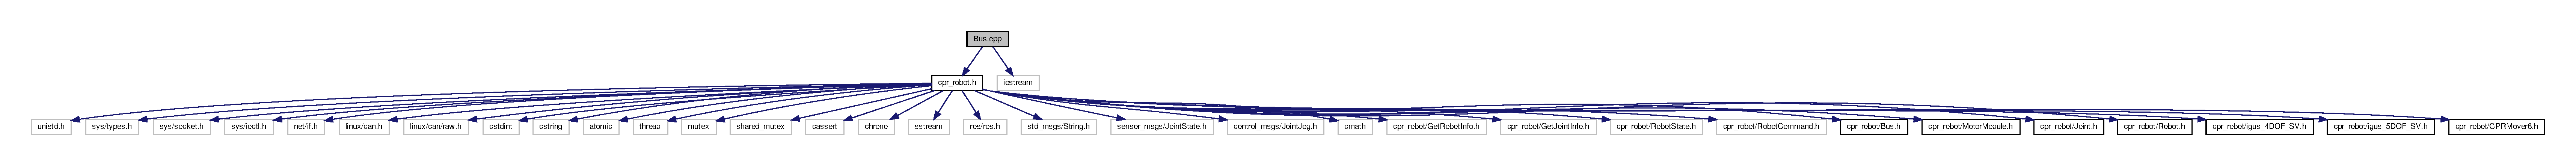
\includegraphics[width=350pt]{Bus_8cpp__incl}
\end{center}
\end{figure}
\subsection*{Namespaces}
\begin{DoxyCompactItemize}
\item 
 \textbf{ cpr\+\_\+robot}
\begin{DoxyCompactList}\small\item\em Provides everything needed to control a robot over a C\+AN bus connection within a R\+OS environment. \end{DoxyCompactList}\end{DoxyCompactItemize}

\section{Bus.\+h File Reference}
\label{Bus_8h}\index{Bus.\+h@{Bus.\+h}}
This graph shows which files directly or indirectly include this file\+:
\nopagebreak
\begin{figure}[H]
\begin{center}
\leavevmode
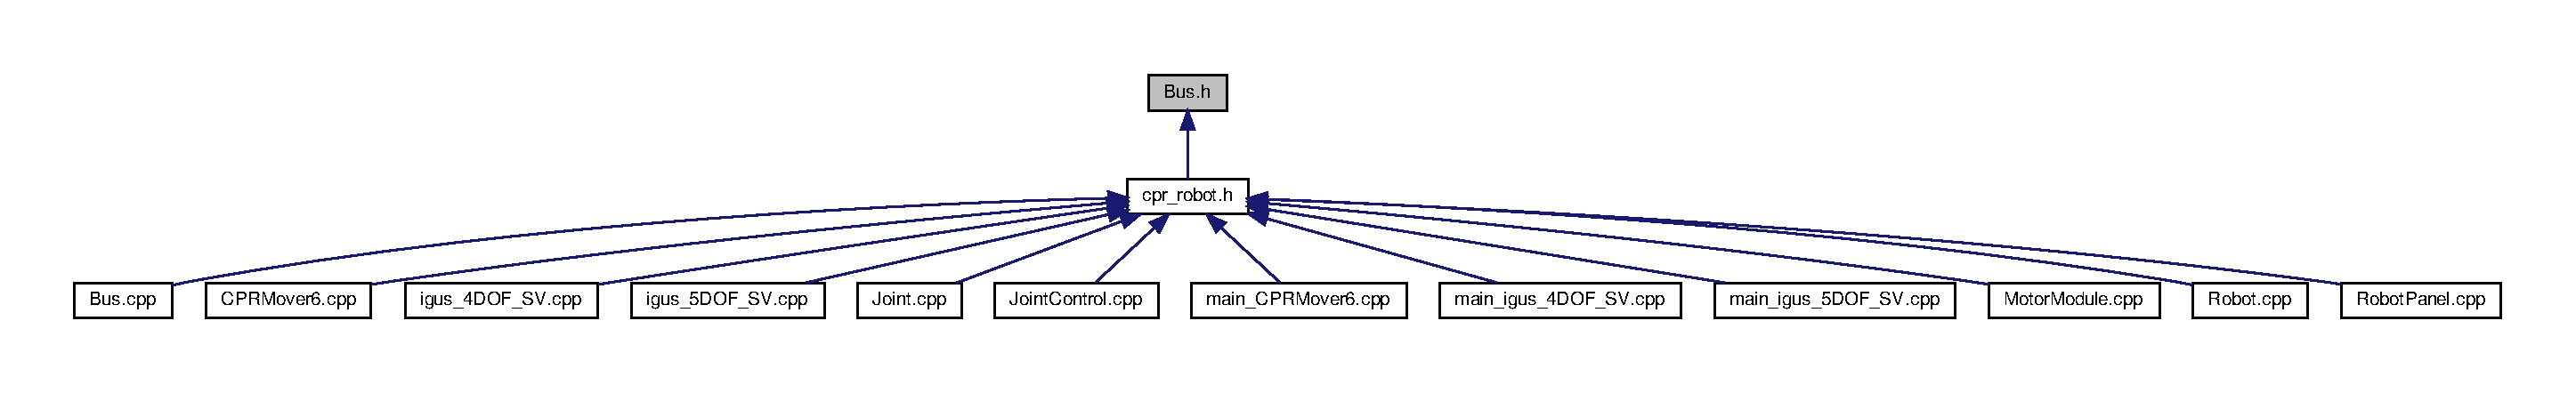
\includegraphics[width=350pt]{Bus_8h__dep__incl}
\end{center}
\end{figure}
\subsection*{Classes}
\begin{DoxyCompactItemize}
\item 
class \textbf{ cpr\+\_\+robot\+::\+Bus}
\begin{DoxyCompactList}\small\item\em Used for communication over the C\+AN bus. \end{DoxyCompactList}\end{DoxyCompactItemize}
\subsection*{Namespaces}
\begin{DoxyCompactItemize}
\item 
 \textbf{ cpr\+\_\+robot}
\begin{DoxyCompactList}\small\item\em Provides everything needed to control a robot over a C\+AN bus connection within a R\+OS environment. \end{DoxyCompactList}\end{DoxyCompactItemize}

\section{cpr\+\_\+robot.\+h File Reference}
\label{cpr__robot_8h}\index{cpr\+\_\+robot.\+h@{cpr\+\_\+robot.\+h}}
{\ttfamily \#include $<$unistd.\+h$>$}\newline
{\ttfamily \#include $<$sys/types.\+h$>$}\newline
{\ttfamily \#include $<$sys/socket.\+h$>$}\newline
{\ttfamily \#include $<$sys/ioctl.\+h$>$}\newline
{\ttfamily \#include $<$net/if.\+h$>$}\newline
{\ttfamily \#include $<$linux/can.\+h$>$}\newline
{\ttfamily \#include $<$linux/can/raw.\+h$>$}\newline
{\ttfamily \#include $<$cstdint$>$}\newline
{\ttfamily \#include $<$cstring$>$}\newline
{\ttfamily \#include $<$atomic$>$}\newline
{\ttfamily \#include $<$thread$>$}\newline
{\ttfamily \#include $<$mutex$>$}\newline
{\ttfamily \#include $<$shared\+\_\+mutex$>$}\newline
{\ttfamily \#include $<$cassert$>$}\newline
{\ttfamily \#include $<$chrono$>$}\newline
{\ttfamily \#include $<$sstream$>$}\newline
{\ttfamily \#include $<$ros/ros.\+h$>$}\newline
{\ttfamily \#include $<$std\+\_\+msgs/\+String.\+h$>$}\newline
{\ttfamily \#include $<$sensor\+\_\+msgs/\+Joint\+State.\+h$>$}\newline
{\ttfamily \#include $<$control\+\_\+msgs/\+Joint\+Jog.\+h$>$}\newline
{\ttfamily \#include $<$cmath$>$}\newline
{\ttfamily \#include \char`\"{}cpr\+\_\+robot/\+Get\+Robot\+Info.\+h\char`\"{}}\newline
{\ttfamily \#include \char`\"{}cpr\+\_\+robot/\+Get\+Joint\+Info.\+h\char`\"{}}\newline
{\ttfamily \#include \char`\"{}cpr\+\_\+robot/\+Robot\+State.\+h\char`\"{}}\newline
{\ttfamily \#include \char`\"{}cpr\+\_\+robot/\+Robot\+Command.\+h\char`\"{}}\newline
{\ttfamily \#include \char`\"{}cpr\+\_\+robot/\+Bus.\+h\char`\"{}}\newline
{\ttfamily \#include \char`\"{}cpr\+\_\+robot/\+Motor\+Module.\+h\char`\"{}}\newline
{\ttfamily \#include \char`\"{}cpr\+\_\+robot/\+Joint.\+h\char`\"{}}\newline
{\ttfamily \#include \char`\"{}cpr\+\_\+robot/\+Robot.\+h\char`\"{}}\newline
{\ttfamily \#include \char`\"{}cpr\+\_\+robot/igus\+\_\+4\+D\+O\+F\+\_\+\+S\+V.\+h\char`\"{}}\newline
{\ttfamily \#include \char`\"{}cpr\+\_\+robot/igus\+\_\+5\+D\+O\+F\+\_\+\+S\+V.\+h\char`\"{}}\newline
{\ttfamily \#include \char`\"{}cpr\+\_\+robot/\+C\+P\+R\+Mover6.\+h\char`\"{}}\newline
Include dependency graph for cpr\+\_\+robot.\+h\+:
\nopagebreak
\begin{figure}[H]
\begin{center}
\leavevmode
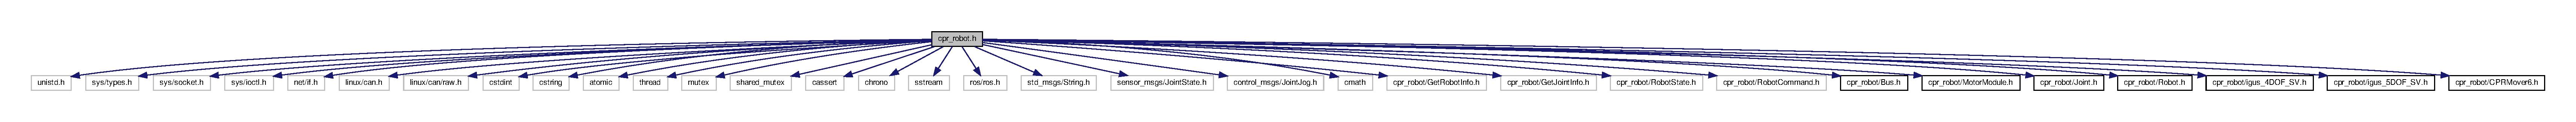
\includegraphics[width=350pt]{cpr__robot_8h__incl}
\end{center}
\end{figure}
This graph shows which files directly or indirectly include this file\+:
\nopagebreak
\begin{figure}[H]
\begin{center}
\leavevmode
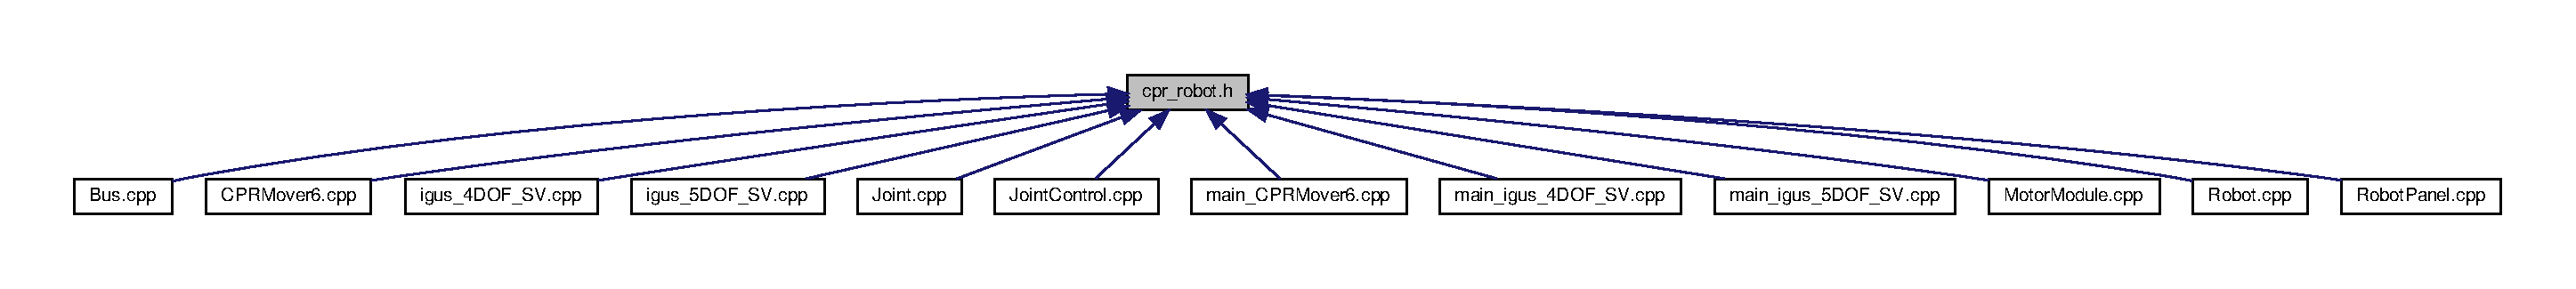
\includegraphics[width=350pt]{cpr__robot_8h__dep__incl}
\end{center}
\end{figure}
\subsection*{Namespaces}
\begin{DoxyCompactItemize}
\item 
 \textbf{ cpr\+\_\+robot}
\begin{DoxyCompactList}\small\item\em Provides everything needed to control a robot over a C\+AN bus connection within a R\+OS environment. \end{DoxyCompactList}\end{DoxyCompactItemize}
\subsection*{Macros}
\begin{DoxyCompactItemize}
\item 
\#define \textbf{ \+\_\+\+U\+S\+E\+\_\+\+M\+A\+T\+H\+\_\+\+D\+E\+F\+I\+N\+ES}
\item 
\#define \textbf{ A\+F\+\_\+\+C\+AN}~\textbf{ P\+F\+\_\+\+C\+AN}
\item 
\#define \textbf{ P\+F\+\_\+\+C\+AN}~29
\end{DoxyCompactItemize}


\subsection{Macro Definition Documentation}
\mbox{\label{cpr__robot_8h_a525335710b53cb064ca56b936120431e}} 
\index{cpr\+\_\+robot.\+h@{cpr\+\_\+robot.\+h}!\+\_\+\+U\+S\+E\+\_\+\+M\+A\+T\+H\+\_\+\+D\+E\+F\+I\+N\+ES@{\+\_\+\+U\+S\+E\+\_\+\+M\+A\+T\+H\+\_\+\+D\+E\+F\+I\+N\+ES}}
\index{\+\_\+\+U\+S\+E\+\_\+\+M\+A\+T\+H\+\_\+\+D\+E\+F\+I\+N\+ES@{\+\_\+\+U\+S\+E\+\_\+\+M\+A\+T\+H\+\_\+\+D\+E\+F\+I\+N\+ES}!cpr\+\_\+robot.\+h@{cpr\+\_\+robot.\+h}}
\subsubsection{\+\_\+\+U\+S\+E\+\_\+\+M\+A\+T\+H\+\_\+\+D\+E\+F\+I\+N\+ES}
{\footnotesize\ttfamily \#define \+\_\+\+U\+S\+E\+\_\+\+M\+A\+T\+H\+\_\+\+D\+E\+F\+I\+N\+ES}



Definition at line 34 of file cpr\+\_\+robot.\+h.

\mbox{\label{cpr__robot_8h_a546620c7e758f003b24b7fdae4f97bd4}} 
\index{cpr\+\_\+robot.\+h@{cpr\+\_\+robot.\+h}!A\+F\+\_\+\+C\+AN@{A\+F\+\_\+\+C\+AN}}
\index{A\+F\+\_\+\+C\+AN@{A\+F\+\_\+\+C\+AN}!cpr\+\_\+robot.\+h@{cpr\+\_\+robot.\+h}}
\subsubsection{A\+F\+\_\+\+C\+AN}
{\footnotesize\ttfamily \#define A\+F\+\_\+\+C\+AN~\textbf{ P\+F\+\_\+\+C\+AN}}



Definition at line 26 of file cpr\+\_\+robot.\+h.

\mbox{\label{cpr__robot_8h_aeac0c3db7a1e021f17987bcc76893849}} 
\index{cpr\+\_\+robot.\+h@{cpr\+\_\+robot.\+h}!P\+F\+\_\+\+C\+AN@{P\+F\+\_\+\+C\+AN}}
\index{P\+F\+\_\+\+C\+AN@{P\+F\+\_\+\+C\+AN}!cpr\+\_\+robot.\+h@{cpr\+\_\+robot.\+h}}
\subsubsection{P\+F\+\_\+\+C\+AN}
{\footnotesize\ttfamily \#define P\+F\+\_\+\+C\+AN~29}



Definition at line 22 of file cpr\+\_\+robot.\+h.


\section{C\+P\+R\+Mover6.\+cpp File Reference}
\label{CPRMover6_8cpp}\index{C\+P\+R\+Mover6.\+cpp@{C\+P\+R\+Mover6.\+cpp}}
{\ttfamily \#include $<$cpr\+\_\+robot.\+h$>$}\newline
Include dependency graph for C\+P\+R\+Mover6.\+cpp\+:
\nopagebreak
\begin{figure}[H]
\begin{center}
\leavevmode
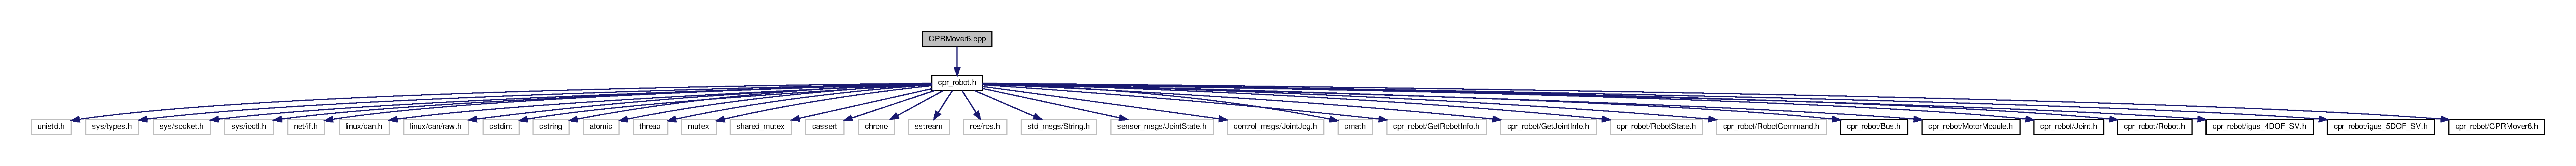
\includegraphics[width=350pt]{CPRMover6_8cpp__incl}
\end{center}
\end{figure}
\subsection*{Namespaces}
\begin{DoxyCompactItemize}
\item 
 \textbf{ cpr\+\_\+robot}
\begin{DoxyCompactList}\small\item\em Provides everything needed to control a robot over a C\+AN bus connection within a R\+OS environment. \end{DoxyCompactList}\end{DoxyCompactItemize}

\section{C\+P\+R\+Mover6.\+h File Reference}
\label{CPRMover6_8h}\index{C\+P\+R\+Mover6.\+h@{C\+P\+R\+Mover6.\+h}}
This graph shows which files directly or indirectly include this file\+:
\nopagebreak
\begin{figure}[H]
\begin{center}
\leavevmode
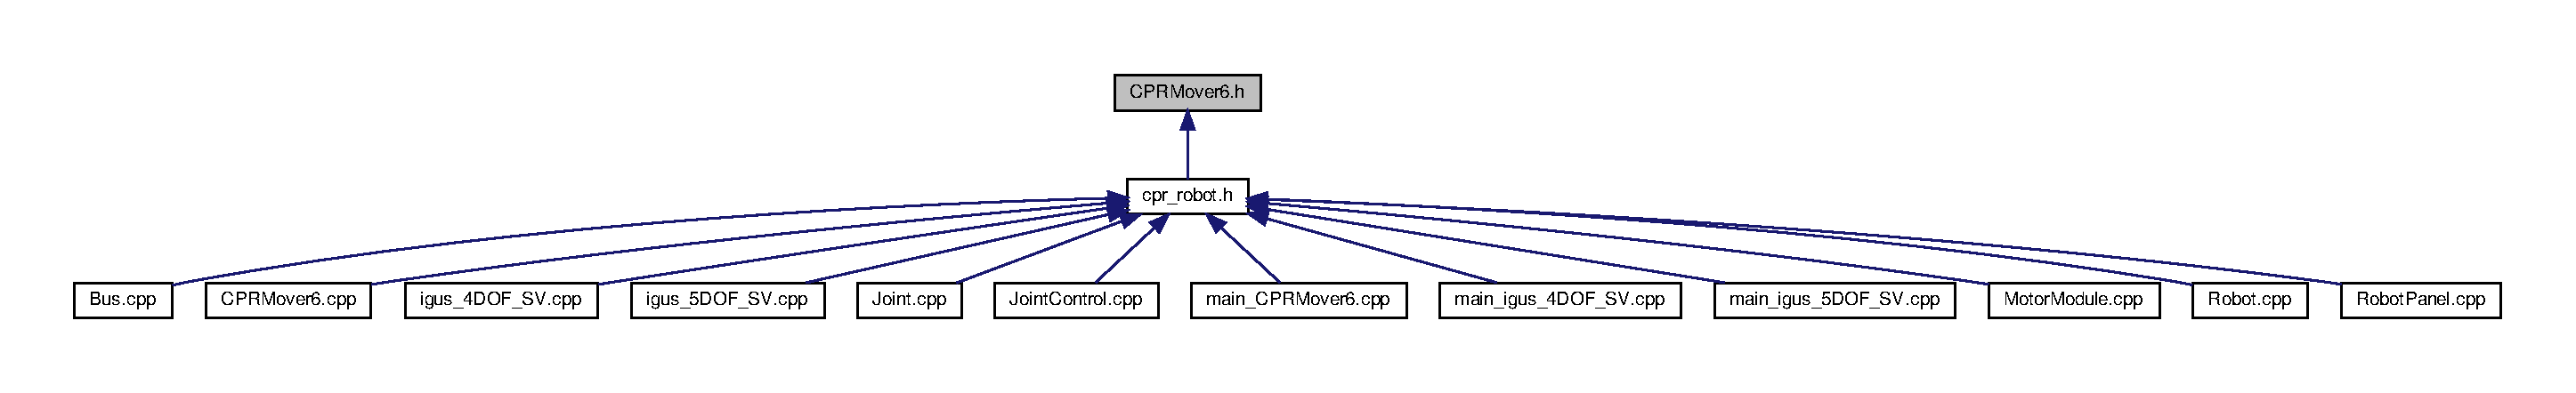
\includegraphics[width=350pt]{CPRMover6_8h__dep__incl}
\end{center}
\end{figure}
\subsection*{Classes}
\begin{DoxyCompactItemize}
\item 
class \textbf{ cpr\+\_\+robot\+::\+C\+P\+R\+Mover6}
\begin{DoxyCompactList}\small\item\em Class representing a Mover6 robot from Commonplace Robotics GmbH. \end{DoxyCompactList}\end{DoxyCompactItemize}
\subsection*{Namespaces}
\begin{DoxyCompactItemize}
\item 
 \textbf{ cpr\+\_\+robot}
\begin{DoxyCompactList}\small\item\em Provides everything needed to control a robot over a C\+AN bus connection within a R\+OS environment. \end{DoxyCompactList}\end{DoxyCompactItemize}

\section{igus\+\_\+4\+D\+O\+F\+\_\+\+S\+V.\+cpp File Reference}
\label{igus__4DOF__SV_8cpp}\index{igus\+\_\+4\+D\+O\+F\+\_\+\+S\+V.\+cpp@{igus\+\_\+4\+D\+O\+F\+\_\+\+S\+V.\+cpp}}
{\ttfamily \#include $<$cpr\+\_\+robot.\+h$>$}\newline
Include dependency graph for igus\+\_\+4\+D\+O\+F\+\_\+\+S\+V.\+cpp\+:
\nopagebreak
\begin{figure}[H]
\begin{center}
\leavevmode
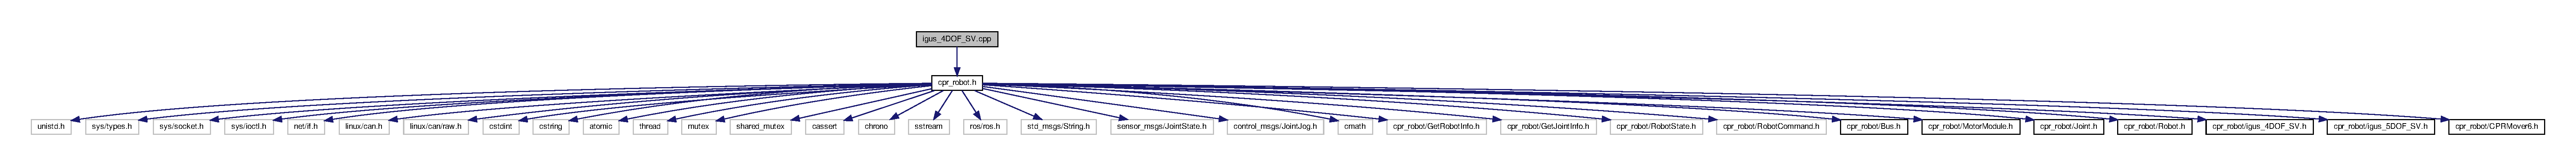
\includegraphics[width=350pt]{igus__4DOF__SV_8cpp__incl}
\end{center}
\end{figure}
\subsection*{Namespaces}
\begin{DoxyCompactItemize}
\item 
 \textbf{ cpr\+\_\+robot}
\begin{DoxyCompactList}\small\item\em Provides everything needed to control a robot over a C\+AN bus connection within a R\+OS environment. \end{DoxyCompactList}\end{DoxyCompactItemize}

\section{igus\+\_\+4\+D\+O\+F\+\_\+\+S\+V.\+h File Reference}
\label{igus__4DOF__SV_8h}\index{igus\+\_\+4\+D\+O\+F\+\_\+\+S\+V.\+h@{igus\+\_\+4\+D\+O\+F\+\_\+\+S\+V.\+h}}
This graph shows which files directly or indirectly include this file\+:
\nopagebreak
\begin{figure}[H]
\begin{center}
\leavevmode
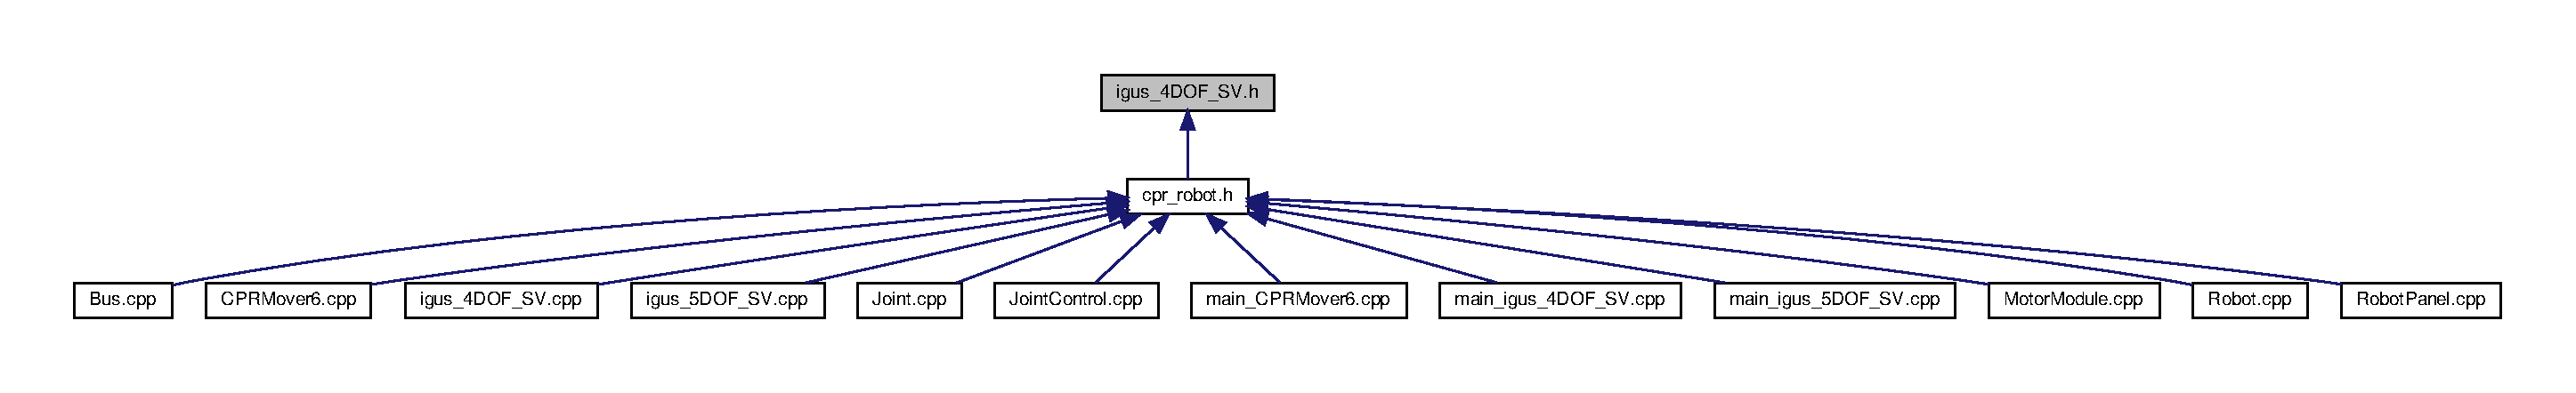
\includegraphics[width=350pt]{igus__4DOF__SV_8h__dep__incl}
\end{center}
\end{figure}
\subsection*{Classes}
\begin{DoxyCompactItemize}
\item 
class \textbf{ cpr\+\_\+robot\+::igus\+\_\+4\+D\+O\+F\+\_\+\+SV}
\begin{DoxyCompactList}\small\item\em Class representing a robolink 4\+D\+OF small version robot from igus. \end{DoxyCompactList}\end{DoxyCompactItemize}
\subsection*{Namespaces}
\begin{DoxyCompactItemize}
\item 
 \textbf{ cpr\+\_\+robot}
\begin{DoxyCompactList}\small\item\em Provides everything needed to control a robot over a C\+AN bus connection within a R\+OS environment. \end{DoxyCompactList}\end{DoxyCompactItemize}

\section{igus\+\_\+5\+D\+O\+F\+\_\+\+S\+V.\+cpp File Reference}
\label{igus__5DOF__SV_8cpp}\index{igus\+\_\+5\+D\+O\+F\+\_\+\+S\+V.\+cpp@{igus\+\_\+5\+D\+O\+F\+\_\+\+S\+V.\+cpp}}
{\ttfamily \#include $<$cpr\+\_\+robot.\+h$>$}\newline
Include dependency graph for igus\+\_\+5\+D\+O\+F\+\_\+\+S\+V.\+cpp\+:
\nopagebreak
\begin{figure}[H]
\begin{center}
\leavevmode
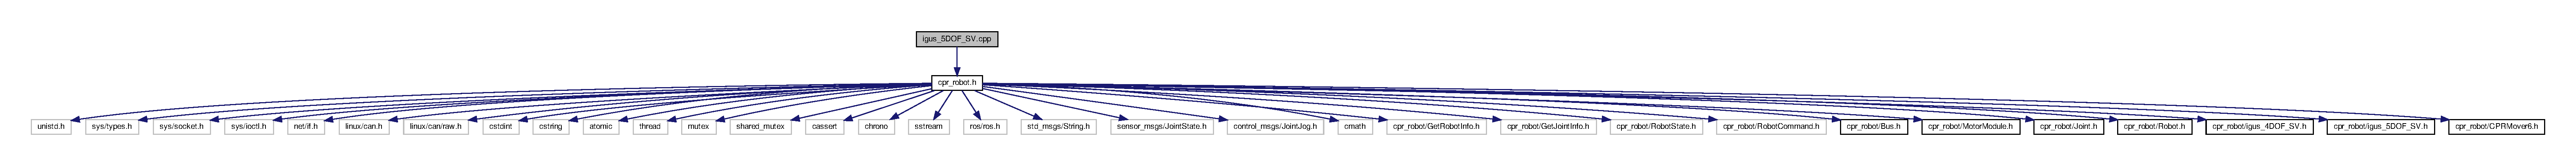
\includegraphics[width=350pt]{igus__5DOF__SV_8cpp__incl}
\end{center}
\end{figure}
\subsection*{Namespaces}
\begin{DoxyCompactItemize}
\item 
 \textbf{ cpr\+\_\+robot}
\begin{DoxyCompactList}\small\item\em Provides everything needed to control a robot over a C\+AN bus connection within a R\+OS environment. \end{DoxyCompactList}\end{DoxyCompactItemize}

\section{igus\+\_\+5\+D\+O\+F\+\_\+\+S\+V.\+h File Reference}
\label{igus__5DOF__SV_8h}\index{igus\+\_\+5\+D\+O\+F\+\_\+\+S\+V.\+h@{igus\+\_\+5\+D\+O\+F\+\_\+\+S\+V.\+h}}
This graph shows which files directly or indirectly include this file\+:
\nopagebreak
\begin{figure}[H]
\begin{center}
\leavevmode
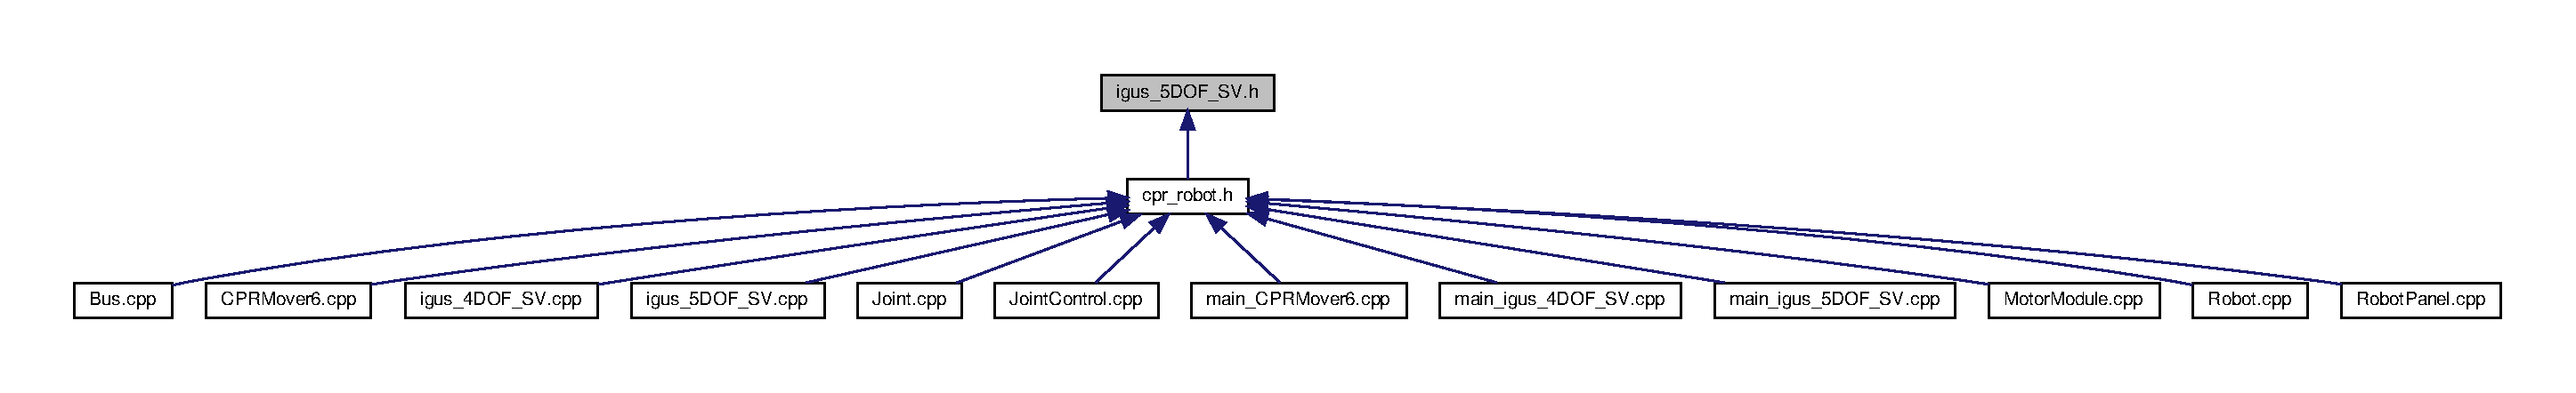
\includegraphics[width=350pt]{igus__5DOF__SV_8h__dep__incl}
\end{center}
\end{figure}
\subsection*{Classes}
\begin{DoxyCompactItemize}
\item 
class \textbf{ cpr\+\_\+robot\+::igus\+\_\+5\+D\+O\+F\+\_\+\+SV}
\begin{DoxyCompactList}\small\item\em Class representing a robolink 5\+D\+OF small version robot from igus. \end{DoxyCompactList}\end{DoxyCompactItemize}
\subsection*{Namespaces}
\begin{DoxyCompactItemize}
\item 
 \textbf{ cpr\+\_\+robot}
\begin{DoxyCompactList}\small\item\em Provides everything needed to control a robot over a C\+AN bus connection within a R\+OS environment. \end{DoxyCompactList}\end{DoxyCompactItemize}

\section{Joint.\+cpp File Reference}
\label{Joint_8cpp}\index{Joint.\+cpp@{Joint.\+cpp}}
{\ttfamily \#include $<$cpr\+\_\+robot.\+h$>$}\newline
{\ttfamily \#include $<$iostream$>$}\newline
{\ttfamily \#include $<$sstream$>$}\newline
Include dependency graph for Joint.\+cpp\+:
\nopagebreak
\begin{figure}[H]
\begin{center}
\leavevmode
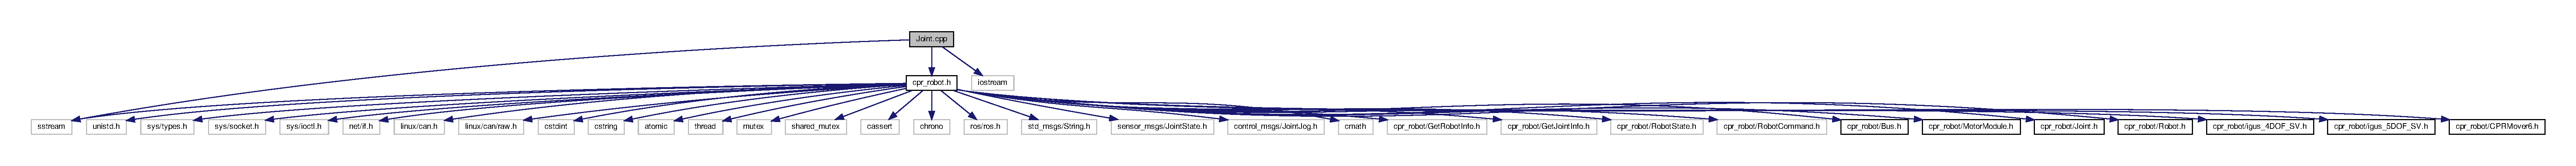
\includegraphics[width=350pt]{Joint_8cpp__incl}
\end{center}
\end{figure}
\subsection*{Namespaces}
\begin{DoxyCompactItemize}
\item 
 \textbf{ cpr\+\_\+robot}
\begin{DoxyCompactList}\small\item\em Provides everything needed to control a robot over a C\+AN bus connection within a R\+OS environment. \end{DoxyCompactList}\end{DoxyCompactItemize}

\section{Joint.\+h File Reference}
\label{Joint_8h}\index{Joint.\+h@{Joint.\+h}}
This graph shows which files directly or indirectly include this file\+:
\nopagebreak
\begin{figure}[H]
\begin{center}
\leavevmode
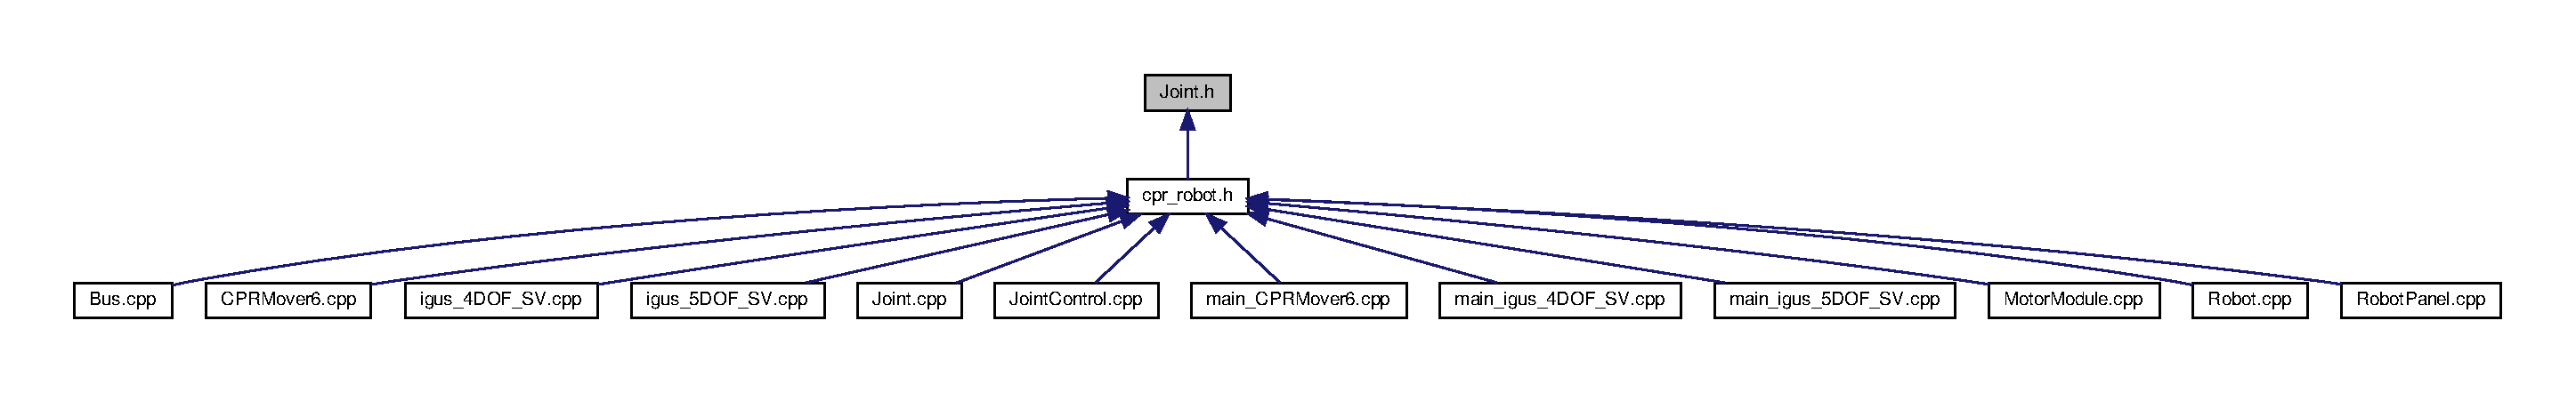
\includegraphics[width=350pt]{Joint_8h__dep__incl}
\end{center}
\end{figure}
\subsection*{Classes}
\begin{DoxyCompactItemize}
\item 
class \textbf{ cpr\+\_\+robot\+::\+Joint}
\begin{DoxyCompactList}\small\item\em Represents a single joint of a robot. \end{DoxyCompactList}\end{DoxyCompactItemize}
\subsection*{Namespaces}
\begin{DoxyCompactItemize}
\item 
 \textbf{ cpr\+\_\+robot}
\begin{DoxyCompactList}\small\item\em Provides everything needed to control a robot over a C\+AN bus connection within a R\+OS environment. \end{DoxyCompactList}\end{DoxyCompactItemize}

\section{Joint\+Control.\+cpp File Reference}
\label{JointControl_8cpp}\index{Joint\+Control.\+cpp@{Joint\+Control.\+cpp}}
{\ttfamily \#include $<$cpr\+\_\+robot.\+h$>$}\newline
{\ttfamily \#include \char`\"{}qt\+\_\+includes.\+h\char`\"{}}\newline
{\ttfamily \#include \char`\"{}Joint\+Control.\+h\char`\"{}}\newline
{\ttfamily \#include $<$sstream$>$}\newline
{\ttfamily \#include $<$iomanip$>$}\newline
{\ttfamily \#include \char`\"{}moc\+\_\+\+Joint\+Control.\+cpp\char`\"{}}\newline
Include dependency graph for Joint\+Control.\+cpp\+:
\nopagebreak
\begin{figure}[H]
\begin{center}
\leavevmode
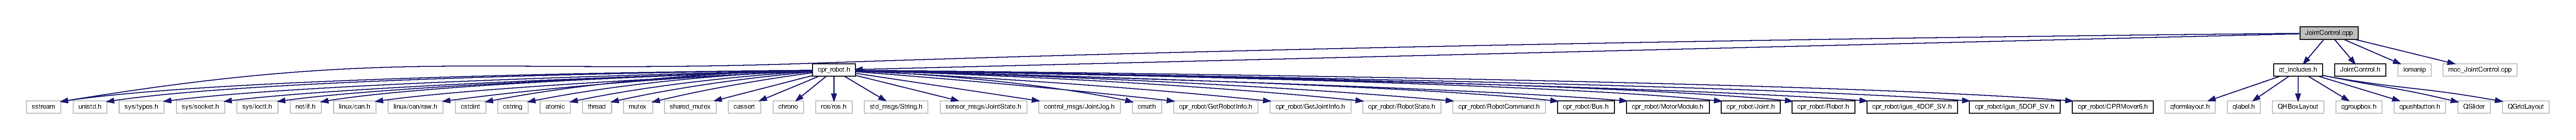
\includegraphics[width=350pt]{JointControl_8cpp__incl}
\end{center}
\end{figure}
\subsection*{Namespaces}
\begin{DoxyCompactItemize}
\item 
 \textbf{ cpr\+\_\+rviz}
\begin{DoxyCompactList}\small\item\em Provides classes defining a plugin for R\+Viz. \end{DoxyCompactList}\end{DoxyCompactItemize}

\section{Joint\+Control.\+h File Reference}
\label{JointControl_8h}\index{Joint\+Control.\+h@{Joint\+Control.\+h}}
This graph shows which files directly or indirectly include this file\+:
\nopagebreak
\begin{figure}[H]
\begin{center}
\leavevmode
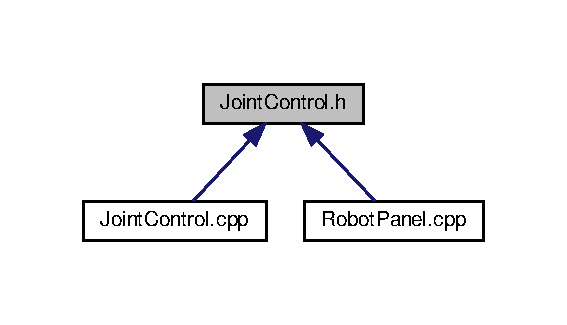
\includegraphics[width=272pt]{JointControl_8h__dep__incl}
\end{center}
\end{figure}
\subsection*{Classes}
\begin{DoxyCompactItemize}
\item 
class \textbf{ cpr\+\_\+rviz\+::\+Joint\+Control}
\begin{DoxyCompactList}\small\item\em Widget that provides motion control for a single robot joint. \end{DoxyCompactList}\end{DoxyCompactItemize}
\subsection*{Namespaces}
\begin{DoxyCompactItemize}
\item 
 \textbf{ cpr\+\_\+rviz}
\begin{DoxyCompactList}\small\item\em Provides classes defining a plugin for R\+Viz. \end{DoxyCompactList}\end{DoxyCompactItemize}

\section{main\+\_\+\+C\+P\+R\+Mover6.\+cpp File Reference}
\label{main__CPRMover6_8cpp}\index{main\+\_\+\+C\+P\+R\+Mover6.\+cpp@{main\+\_\+\+C\+P\+R\+Mover6.\+cpp}}
{\ttfamily \#include $<$cpr\+\_\+robot.\+h$>$}\newline
{\ttfamily \#include $<$sstream$>$}\newline
{\ttfamily \#include $<$cmath$>$}\newline
Include dependency graph for main\+\_\+\+C\+P\+R\+Mover6.\+cpp\+:
\nopagebreak
\begin{figure}[H]
\begin{center}
\leavevmode
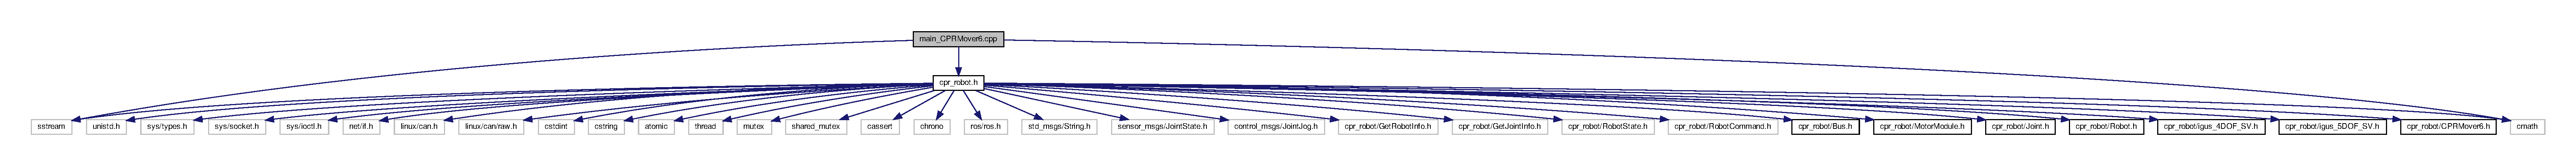
\includegraphics[width=350pt]{main__CPRMover6_8cpp__incl}
\end{center}
\end{figure}
\subsection*{Functions}
\begin{DoxyCompactItemize}
\item 
int \textbf{ main} (int argc, char $\ast$$\ast$argv)
\end{DoxyCompactItemize}


\subsection{Function Documentation}
\mbox{\label{main__CPRMover6_8cpp_a3c04138a5bfe5d72780bb7e82a18e627}} 
\index{main\+\_\+\+C\+P\+R\+Mover6.\+cpp@{main\+\_\+\+C\+P\+R\+Mover6.\+cpp}!main@{main}}
\index{main@{main}!main\+\_\+\+C\+P\+R\+Mover6.\+cpp@{main\+\_\+\+C\+P\+R\+Mover6.\+cpp}}
\subsubsection{main()}
{\footnotesize\ttfamily int main (\begin{DoxyParamCaption}\item[{int}]{argc,  }\item[{char $\ast$$\ast$}]{argv }\end{DoxyParamCaption})}

This tutorial demonstrates simple sending of messages over the R\+OS system. The ros\+::init() function needs to see argc and argv so that it can perform any R\+OS arguments and name remapping that were provided at the command line. For programmatic remappings you can use a different version of init() which takes remappings directly, but for most command-\/line programs, passing argc and argv is the easiest way to do it. The third argument to init() is the name of the node.

You must call one of the versions of ros\+::init() before using any other part of the R\+OS system.

Node\+Handle is the main access point to communications with the R\+OS system. The first Node\+Handle constructed will fully initialize this node, and the last Node\+Handle destructed will close down the node.

A count of how many messages we have sent. This is used to create a unique string for each message.

This is a message object. You stuff it with data, and then publish it.

Definition at line 8 of file main\+\_\+\+C\+P\+R\+Mover6.\+cpp.


\section{main\+\_\+igus\+\_\+4\+D\+O\+F\+\_\+\+S\+V.\+cpp File Reference}
\label{main__igus__4DOF__SV_8cpp}\index{main\+\_\+igus\+\_\+4\+D\+O\+F\+\_\+\+S\+V.\+cpp@{main\+\_\+igus\+\_\+4\+D\+O\+F\+\_\+\+S\+V.\+cpp}}
{\ttfamily \#include $<$cpr\+\_\+robot.\+h$>$}\newline
{\ttfamily \#include $<$sstream$>$}\newline
{\ttfamily \#include $<$cmath$>$}\newline
Include dependency graph for main\+\_\+igus\+\_\+4\+D\+O\+F\+\_\+\+S\+V.\+cpp\+:
\nopagebreak
\begin{figure}[H]
\begin{center}
\leavevmode
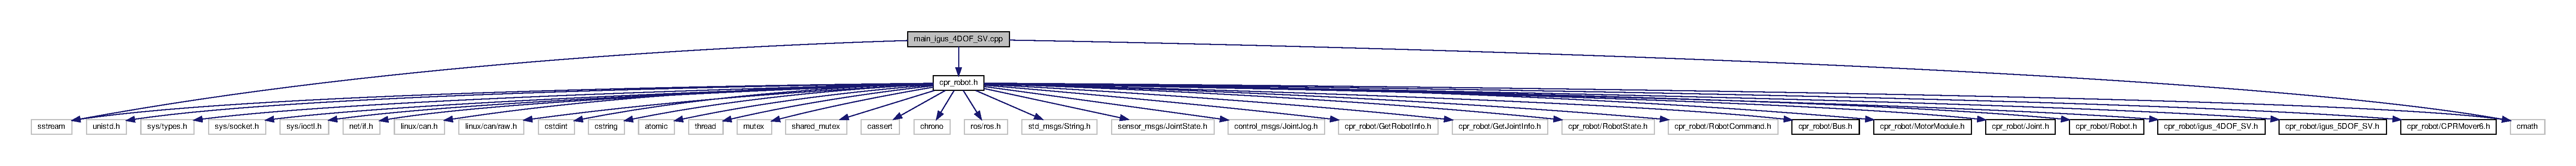
\includegraphics[width=350pt]{main__igus__4DOF__SV_8cpp__incl}
\end{center}
\end{figure}
\subsection*{Functions}
\begin{DoxyCompactItemize}
\item 
int \textbf{ main} (int argc, char $\ast$$\ast$argv)
\end{DoxyCompactItemize}


\subsection{Function Documentation}
\mbox{\label{main__igus__4DOF__SV_8cpp_a3c04138a5bfe5d72780bb7e82a18e627}} 
\index{main\+\_\+igus\+\_\+4\+D\+O\+F\+\_\+\+S\+V.\+cpp@{main\+\_\+igus\+\_\+4\+D\+O\+F\+\_\+\+S\+V.\+cpp}!main@{main}}
\index{main@{main}!main\+\_\+igus\+\_\+4\+D\+O\+F\+\_\+\+S\+V.\+cpp@{main\+\_\+igus\+\_\+4\+D\+O\+F\+\_\+\+S\+V.\+cpp}}
\subsubsection{main()}
{\footnotesize\ttfamily int main (\begin{DoxyParamCaption}\item[{int}]{argc,  }\item[{char $\ast$$\ast$}]{argv }\end{DoxyParamCaption})}

This tutorial demonstrates simple sending of messages over the R\+OS system. The ros\+::init() function needs to see argc and argv so that it can perform any R\+OS arguments and name remapping that were provided at the command line. For programmatic remappings you can use a different version of init() which takes remappings directly, but for most command-\/line programs, passing argc and argv is the easiest way to do it. The third argument to init() is the name of the node.

You must call one of the versions of ros\+::init() before using any other part of the R\+OS system.

Node\+Handle is the main access point to communications with the R\+OS system. The first Node\+Handle constructed will fully initialize this node, and the last Node\+Handle destructed will close down the node.

A count of how many messages we have sent. This is used to create a unique string for each message.

This is a message object. You stuff it with data, and then publish it.

Definition at line 8 of file main\+\_\+igus\+\_\+4\+D\+O\+F\+\_\+\+S\+V.\+cpp.


\section{main\+\_\+igus\+\_\+5\+D\+O\+F\+\_\+\+S\+V.\+cpp File Reference}
\label{main__igus__5DOF__SV_8cpp}\index{main\+\_\+igus\+\_\+5\+D\+O\+F\+\_\+\+S\+V.\+cpp@{main\+\_\+igus\+\_\+5\+D\+O\+F\+\_\+\+S\+V.\+cpp}}
{\ttfamily \#include $<$cpr\+\_\+robot.\+h$>$}\newline
{\ttfamily \#include $<$sstream$>$}\newline
{\ttfamily \#include $<$cmath$>$}\newline
Include dependency graph for main\+\_\+igus\+\_\+5\+D\+O\+F\+\_\+\+S\+V.\+cpp\+:
\nopagebreak
\begin{figure}[H]
\begin{center}
\leavevmode
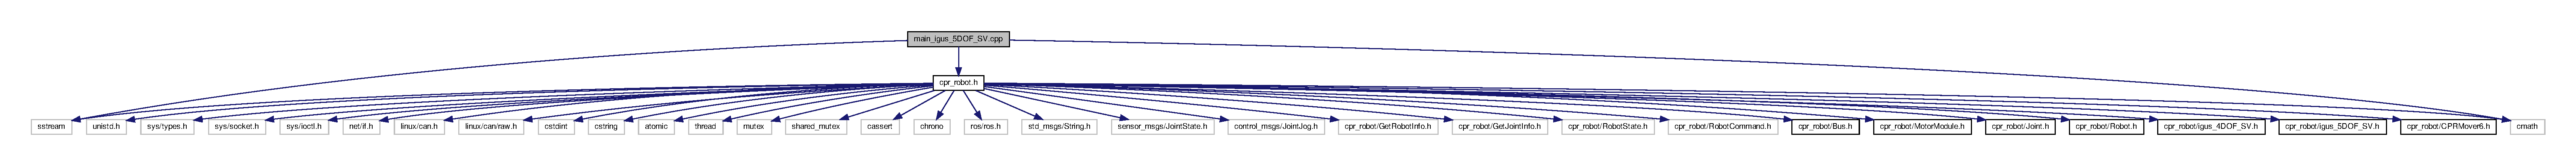
\includegraphics[width=350pt]{main__igus__5DOF__SV_8cpp__incl}
\end{center}
\end{figure}
\subsection*{Functions}
\begin{DoxyCompactItemize}
\item 
int \textbf{ main} (int argc, char $\ast$$\ast$argv)
\end{DoxyCompactItemize}


\subsection{Function Documentation}
\mbox{\label{main__igus__5DOF__SV_8cpp_a3c04138a5bfe5d72780bb7e82a18e627}} 
\index{main\+\_\+igus\+\_\+5\+D\+O\+F\+\_\+\+S\+V.\+cpp@{main\+\_\+igus\+\_\+5\+D\+O\+F\+\_\+\+S\+V.\+cpp}!main@{main}}
\index{main@{main}!main\+\_\+igus\+\_\+5\+D\+O\+F\+\_\+\+S\+V.\+cpp@{main\+\_\+igus\+\_\+5\+D\+O\+F\+\_\+\+S\+V.\+cpp}}
\subsubsection{main()}
{\footnotesize\ttfamily int main (\begin{DoxyParamCaption}\item[{int}]{argc,  }\item[{char $\ast$$\ast$}]{argv }\end{DoxyParamCaption})}

This tutorial demonstrates simple sending of messages over the R\+OS system. The ros\+::init() function needs to see argc and argv so that it can perform any R\+OS arguments and name remapping that were provided at the command line. For programmatic remappings you can use a different version of init() which takes remappings directly, but for most command-\/line programs, passing argc and argv is the easiest way to do it. The third argument to init() is the name of the node.

You must call one of the versions of ros\+::init() before using any other part of the R\+OS system.

Node\+Handle is the main access point to communications with the R\+OS system. The first Node\+Handle constructed will fully initialize this node, and the last Node\+Handle destructed will close down the node.

A count of how many messages we have sent. This is used to create a unique string for each message.

This is a message object. You stuff it with data, and then publish it.

Definition at line 8 of file main\+\_\+igus\+\_\+5\+D\+O\+F\+\_\+\+S\+V.\+cpp.


\section{mainpage.\+dox File Reference}
\label{mainpage_8dox}\index{mainpage.\+dox@{mainpage.\+dox}}

\section{Motor\+Module.\+cpp File Reference}
\label{MotorModule_8cpp}\index{Motor\+Module.\+cpp@{Motor\+Module.\+cpp}}
{\ttfamily \#include $<$cpr\+\_\+robot.\+h$>$}\newline
{\ttfamily \#include $<$iostream$>$}\newline
Include dependency graph for Motor\+Module.\+cpp\+:
\nopagebreak
\begin{figure}[H]
\begin{center}
\leavevmode
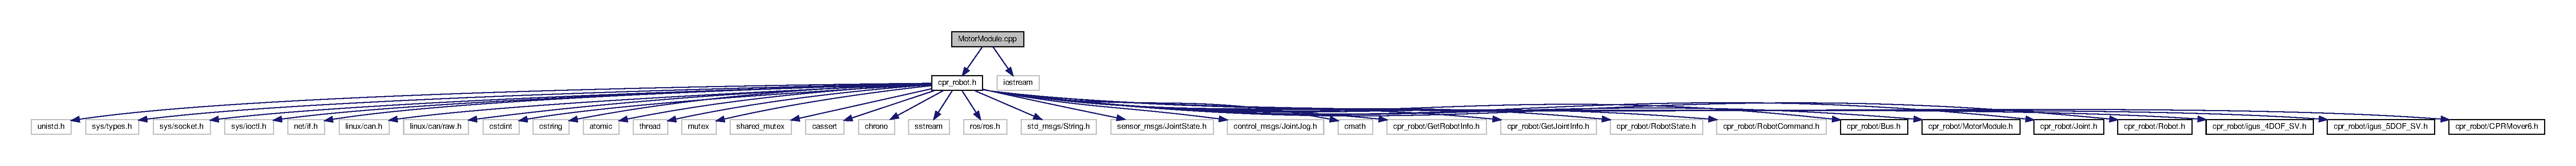
\includegraphics[width=350pt]{MotorModule_8cpp__incl}
\end{center}
\end{figure}
\subsection*{Namespaces}
\begin{DoxyCompactItemize}
\item 
 \textbf{ cpr\+\_\+robot}
\begin{DoxyCompactList}\small\item\em Provides everything needed to control a robot over a C\+AN bus connection within a R\+OS environment. \end{DoxyCompactList}\end{DoxyCompactItemize}

\section{Motor\+Module.\+h File Reference}
\label{MotorModule_8h}\index{Motor\+Module.\+h@{Motor\+Module.\+h}}
This graph shows which files directly or indirectly include this file\+:
\nopagebreak
\begin{figure}[H]
\begin{center}
\leavevmode
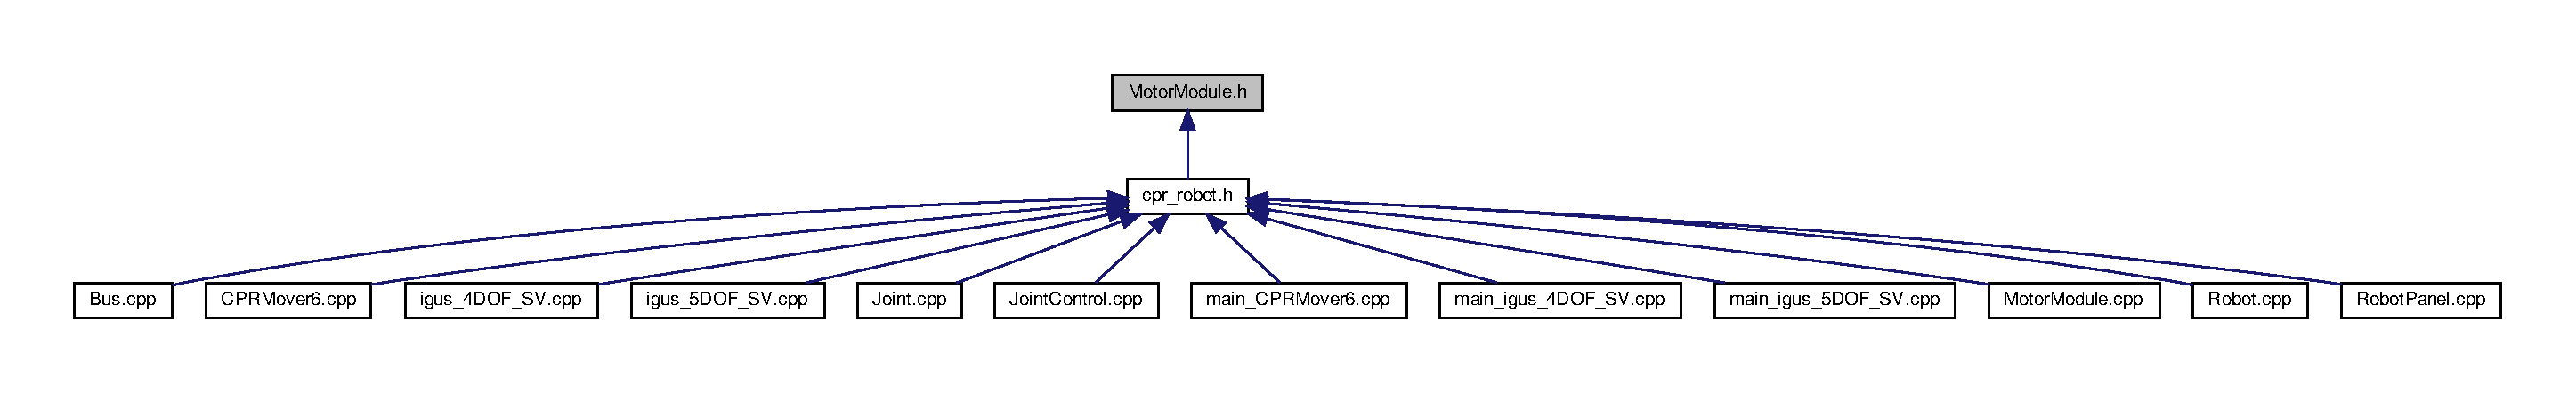
\includegraphics[width=350pt]{MotorModule_8h__dep__incl}
\end{center}
\end{figure}
\subsection*{Classes}
\begin{DoxyCompactItemize}
\item 
class \textbf{ cpr\+\_\+robot\+::\+Motor\+Module}
\begin{DoxyCompactList}\small\item\em Represents a D\+IN rail motorcontrol module from Commonplace Robotics GmbH. \end{DoxyCompactList}\end{DoxyCompactItemize}
\subsection*{Namespaces}
\begin{DoxyCompactItemize}
\item 
 \textbf{ cpr\+\_\+robot}
\begin{DoxyCompactList}\small\item\em Provides everything needed to control a robot over a C\+AN bus connection within a R\+OS environment. \end{DoxyCompactList}\end{DoxyCompactItemize}

\section{qt\+\_\+includes.\+h File Reference}
\label{qt__includes_8h}\index{qt\+\_\+includes.\+h@{qt\+\_\+includes.\+h}}
{\ttfamily \#include $<$qformlayout.\+h$>$}\newline
{\ttfamily \#include $<$qlabel.\+h$>$}\newline
{\ttfamily \#include $<$Q\+H\+Box\+Layout$>$}\newline
{\ttfamily \#include $<$qgroupbox.\+h$>$}\newline
{\ttfamily \#include $<$qpushbutton.\+h$>$}\newline
{\ttfamily \#include $<$Q\+Slider$>$}\newline
{\ttfamily \#include $<$Q\+Grid\+Layout$>$}\newline
Include dependency graph for qt\+\_\+includes.\+h\+:
\nopagebreak
\begin{figure}[H]
\begin{center}
\leavevmode
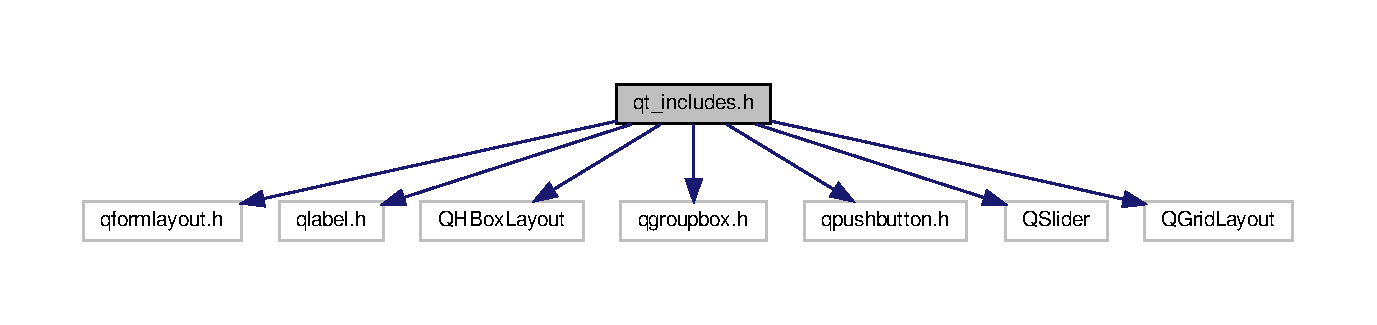
\includegraphics[width=350pt]{qt__includes_8h__incl}
\end{center}
\end{figure}
This graph shows which files directly or indirectly include this file\+:
\nopagebreak
\begin{figure}[H]
\begin{center}
\leavevmode
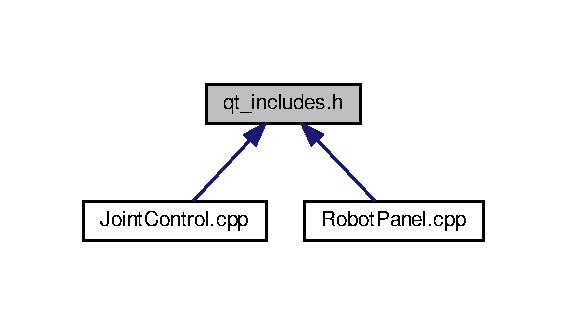
\includegraphics[width=272pt]{qt__includes_8h__dep__incl}
\end{center}
\end{figure}

\section{Robot.\+cpp File Reference}
\label{Robot_8cpp}\index{Robot.\+cpp@{Robot.\+cpp}}
{\ttfamily \#include $<$cpr\+\_\+robot.\+h$>$}\newline
{\ttfamily \#include $<$iostream$>$}\newline
{\ttfamily \#include $<$sstream$>$}\newline
Include dependency graph for Robot.\+cpp\+:
\nopagebreak
\begin{figure}[H]
\begin{center}
\leavevmode
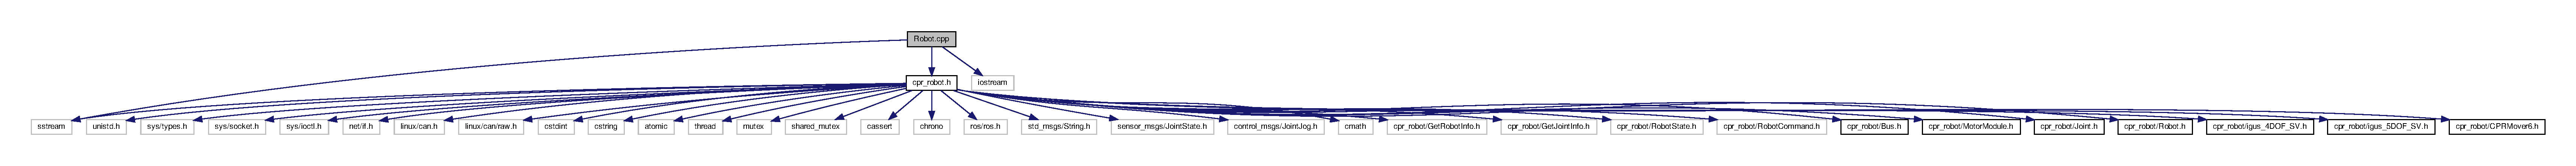
\includegraphics[width=350pt]{Robot_8cpp__incl}
\end{center}
\end{figure}
\subsection*{Namespaces}
\begin{DoxyCompactItemize}
\item 
 \textbf{ cpr\+\_\+robot}
\begin{DoxyCompactList}\small\item\em Provides everything needed to control a robot over a C\+AN bus connection within a R\+OS environment. \end{DoxyCompactList}\end{DoxyCompactItemize}

\section{Robot.\+h File Reference}
\label{Robot_8h}\index{Robot.\+h@{Robot.\+h}}
This graph shows which files directly or indirectly include this file\+:
\nopagebreak
\begin{figure}[H]
\begin{center}
\leavevmode
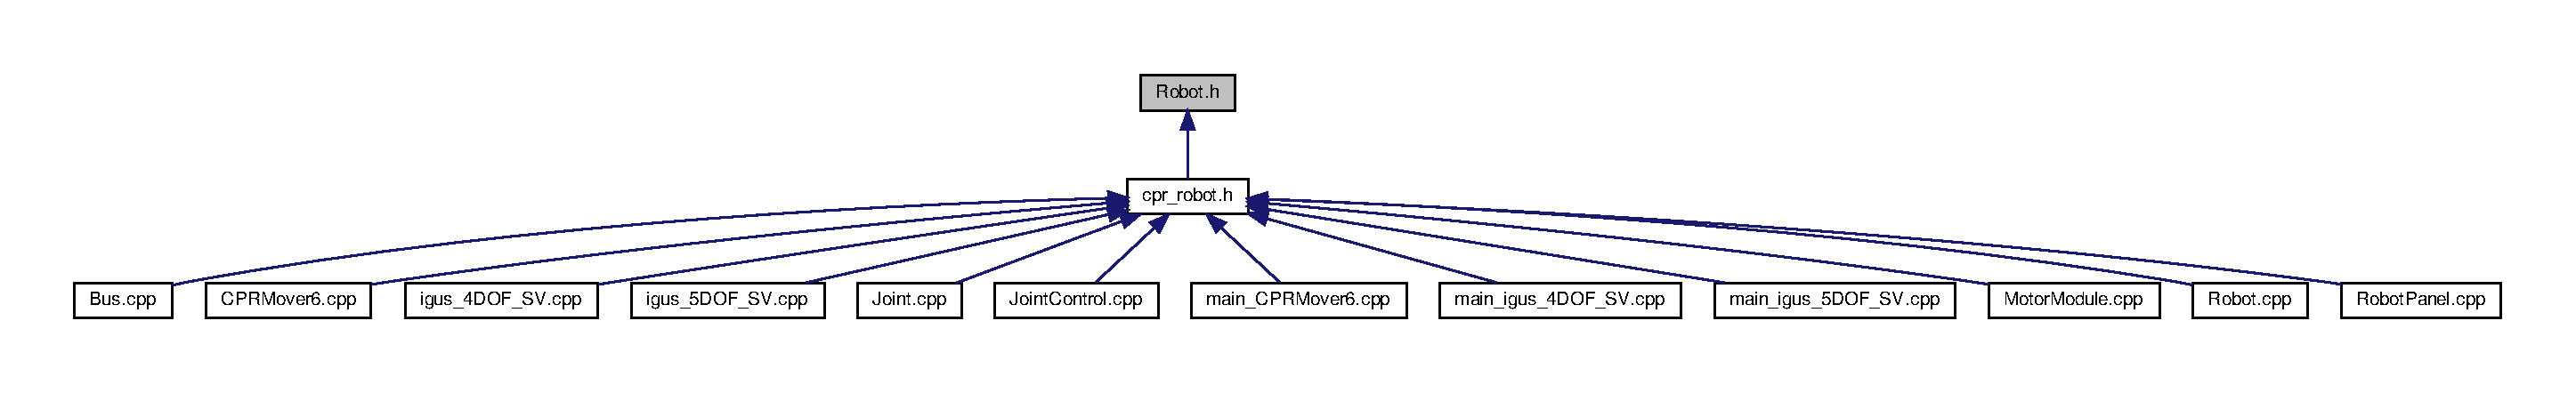
\includegraphics[width=350pt]{Robot_8h__dep__incl}
\end{center}
\end{figure}
\subsection*{Classes}
\begin{DoxyCompactItemize}
\item 
class \textbf{ cpr\+\_\+robot\+::\+Robot}
\begin{DoxyCompactList}\small\item\em Abstract class representing a generic robot. \end{DoxyCompactList}\end{DoxyCompactItemize}
\subsection*{Namespaces}
\begin{DoxyCompactItemize}
\item 
 \textbf{ cpr\+\_\+robot}
\begin{DoxyCompactList}\small\item\em Provides everything needed to control a robot over a C\+AN bus connection within a R\+OS environment. \end{DoxyCompactList}\end{DoxyCompactItemize}

\section{Robot\+Panel.\+cpp File Reference}
\label{RobotPanel_8cpp}\index{Robot\+Panel.\+cpp@{Robot\+Panel.\+cpp}}
{\ttfamily \#include \char`\"{}cpr\+\_\+robot.\+h\char`\"{}}\newline
{\ttfamily \#include \char`\"{}qt\+\_\+includes.\+h\char`\"{}}\newline
{\ttfamily \#include \char`\"{}Joint\+Control.\+h\char`\"{}}\newline
{\ttfamily \#include $<$rviz/panel.\+h$>$}\newline
{\ttfamily \#include \char`\"{}Robot\+Panel.\+h\char`\"{}}\newline
{\ttfamily \#include $<$pluginlib/class\+\_\+list\+\_\+macros.\+h$>$}\newline
{\ttfamily \#include \char`\"{}moc\+\_\+\+Robot\+Panel.\+cpp\char`\"{}}\newline
Include dependency graph for Robot\+Panel.\+cpp\+:
\nopagebreak
\begin{figure}[H]
\begin{center}
\leavevmode
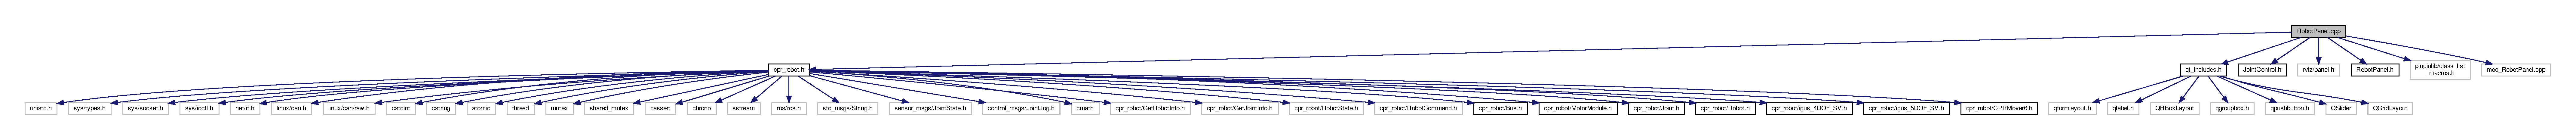
\includegraphics[width=350pt]{RobotPanel_8cpp__incl}
\end{center}
\end{figure}
\subsection*{Namespaces}
\begin{DoxyCompactItemize}
\item 
 \textbf{ cpr\+\_\+rviz}
\begin{DoxyCompactList}\small\item\em Provides classes defining a plugin for R\+Viz. \end{DoxyCompactList}\end{DoxyCompactItemize}

\section{Robot\+Panel.\+h File Reference}
\label{RobotPanel_8h}\index{Robot\+Panel.\+h@{Robot\+Panel.\+h}}
This graph shows which files directly or indirectly include this file\+:
\nopagebreak
\begin{figure}[H]
\begin{center}
\leavevmode
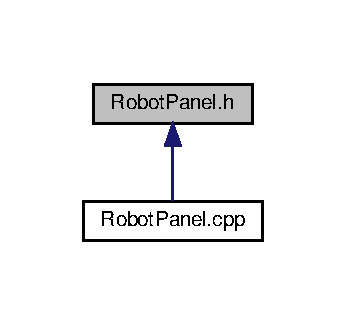
\includegraphics[width=166pt]{RobotPanel_8h__dep__incl}
\end{center}
\end{figure}
\subsection*{Classes}
\begin{DoxyCompactItemize}
\item 
class \textbf{ cpr\+\_\+rviz\+::\+Robot\+Panel}
\begin{DoxyCompactList}\small\item\em Plugin for R\+Viz that allows to move a robot remotely over R\+OS. \end{DoxyCompactList}\end{DoxyCompactItemize}
\subsection*{Namespaces}
\begin{DoxyCompactItemize}
\item 
 \textbf{ cpr\+\_\+rviz}
\begin{DoxyCompactList}\small\item\em Provides classes defining a plugin for R\+Viz. \end{DoxyCompactList}\end{DoxyCompactItemize}

%--- End generated contents ---

% Index
\backmatter
\newpage
\phantomsection
\clearemptydoublepage
\addcontentsline{toc}{chapter}{Index}
\printindex

\end{document}
